% ─────────────────────────────────────────────
% Reader: Data Analysis & Visualisation
% ─────────────────────────────────────────────
\documentclass[12pt, a4paper]{article}

% ── Encoding & language ──────────────────────
\usepackage[utf8]{inputenc}
\usepackage[T1]{fontenc}
\usepackage{lmodern}
\usepackage[english]{babel}

% ── Mathematics ──────────────────────────────
\usepackage{amsmath}
\usepackage{amssymb}
\usepackage{amsthm}
\usepackage{mathtools}

% ── Layout ───────────────────────────────────
\usepackage[margin=2.5cm]{geometry}
\usepackage{parskip}
\usepackage{microtype}
\usepackage{booktabs}
\usepackage{tabularx}
\usepackage{graphicx}
\usepackage{caption}
\usepackage{float}
\usepackage{hyperref}
\usepackage{tikz}
\usetikzlibrary{arrows.meta, calc}

% Figures are the ones from the lesson decks.
\graphicspath{{../presentations/img/}}

% Every subsubsection follows a slide title, so it is listed in the contents.
\setcounter{tocdepth}{3}

% ── Theorem environments ─────────────────────
\theoremstyle{definition}
\newtheorem{definition}{Definition}[section]
\newtheorem{example}{Example}[section]

\theoremstyle{remark}
\newtheorem*{remark}{Remark}
\newtheorem*{note}{Note}

% ── Common shorthands ────────────────────────
\newcommand{\R}{\mathbb{R}}
\newcommand{\N}{\mathbb{N}}
\newcommand{\E}{\mathbb{E}}
\DeclareMathOperator{\Var}{Var}

% The recap that closes each question, as on the "again, concretely" slides.
\newcommand{\againconcretely}{\paragraph{Again, concretely.}}


% ─────────────────────────────────────────────
% Document metadata
% ─────────────────────────────────────────────
\title{Data Analysis \& Visualisation\\[0.3em]\large A reader for MADS-DAV}
\author{Raoul Grouls}
\date{\today}

% ─────────────────────────────────────────────
\begin{document}

\maketitle
\tableofcontents
\newpage

\section{Introduction}
\label{sec:introduction}
This reader accompanies the course Data Analysis \& Visualisation. The slides of each lesson are built to be shown, not read: they carry a plot, a sentence and a question, and the reasoning happens in the room. This reader is where that reasoning is written down, so you can go back to it when you are working on your own data and the lesson is a few weeks behind you.

The course is not a statistics course, and nobody has to become a statistician. What I want you to learn is to \emph{reason} about data: to ask how the numbers in front of you came about, which model of that process makes sense, and what you are allowed to conclude from it. Most mistakes I see in data analysis are not mistakes in the code or in the formulas. They are mistakes in thinking: a model that was chosen without noticing it was a choice, a pattern that was found by looking for it, a title that claims more than the data can carry. A good visualisation is the end of that reasoning, not a replacement for it.

The course runs from visualisation principles and comparing categories, through time, distributions and modelling, to high-dimensional data and dashboards. Each lesson gets its own section in this reader, and a topic that runs through the whole course, such as reading your own code with atlas, gets a section of its own. Each lesson's section follows the deck of that lesson: a subsection per question on the agenda, and a subsubsection per slide with real data, under the title of that slide. You can read the two side by side. Each question ends with the same recap as the deck, ``again, concretely''. The sections are written in the order I need them, so not every lesson is in here yet.
\newpage

\section{Lesson 4: Distributions}
\label{sec:lesson4}
You probably already know the bell curve, the standard deviation and the boxplot. This lesson is about everything else. The lesson is organised around five questions, and I would like you to be able to answer all five at the end of it:

\begin{enumerate}
\item \textbf{What} is a distribution? Chance has rules. A distribution describes them with parameters.
\item \textbf{Which} distribution fits my data? Think about the underlying drivers before you fit.
\item What is an \textbf{outlier}? This depends on the distribution you choose. Choose the wrong one and ordinary values look like outliers.
\item Did something \textbf{change}, or is it chance? Random data always fluctuates. Compare before and after an event, and ask how big a difference chance alone makes.
\item Is my \textbf{model} done? What your model can't explain might tell you whether you missed something.
\end{enumerate}

The first two are about describing data. The last three are about what you can do once you have a description: decide what is unusual, decide whether something really changed, and decide whether your model has captured what is going on.

% ─────────────────────────────────────────────
\subsection{What is a distribution?}
\label{sec:what-is-a-distribution}
You cannot predict a single roll of a die. You can, however, say a lot about a thousand rolls: every face will come up roughly a sixth of the time. Chance is not chaos; chance has rules, and a distribution is a description of those rules: every possible outcome, and how often it happens. Often a few numbers are enough. The bell curve needs a mean and a standard deviation; a count at a steady rate needs only its average. Those numbers are the \emph{parameters} of the distribution.

A distribution is good for three things, and they are the rest of this lesson. It lets you \emph{describe} a random process with just a few parameters. It lets you \emph{judge} what is normal and what is unusual. And it lets you \emph{compare}: two distributions, before and after something happened, tell you whether the mechanism behind a random process has changed.

\subsubsection{Two kinds of not knowing}
It helps to separate two kinds of not knowing. The first is \emph{aleatoric} uncertainty, randomness that is part of the process itself. The word comes from the Latin \textit{alea}, a die\footnote{The oldest dice were astragali, the ankle bones of sheep and goats, which land on one of four sides. The ones on the slide are Greek glass copies from the 3rd--2nd century BC, in the Metropolitan Museum of Art.}. Even if you know everything there is to know about a fair die, you only know how often each face comes up, never which face comes up next. The second is \emph{epistemic} uncertainty: things you could know, but don't (yet). Your travel time is uncertain partly because you haven't checked the traffic. Check it, and that part of the uncertainty shrinks.

Real data always mixes the two. A distribution describes whatever uncertainty is left after you have used what you know, which is why a better model, with more information, gives a narrower distribution. Keep this in mind for the last question of this lesson: a model that looks finished might still be missing knowledge.

\subsubsection{Three rules make something a distribution}
\begin{definition}
\label{def:distribution}
A \emph{probability distribution} assigns a probability to the outcomes of a random process, such that
\begin{enumerate}
\item no outcome has a negative probability;
\item the probabilities over all possible outcomes sum to $1$;
\item the probability of ``this or that'', for outcomes that cannot happen together, is the sum of their probabilities: $P(1 \text{ or } 2) = \tfrac{1}{6} + \tfrac{1}{6}$.
\end{enumerate}
\end{definition}

That is all. A die is \emph{discrete}: it has a finite number of outcomes, and every bar is a probability. For a measurement, such as the flipper length of a penguin, the sum in the third rule becomes an area: the probability that a flipper is between $190$ and $200$ mm is the area under the curve between those values, $0.43$ for Adelie penguins.

\subsubsection{\texorpdfstring{Continuous distributions: there is 0 chance of exactly 21.0\,°C}{Continuous distributions: there is 0 chance of exactly 21.0 °C}}
A measurement such as a temperature is \emph{continuous}, and then something strange happens. Suppose the temperature in a room over the day follows a bell curve with mean $21\,^{\circ}$C and standard deviation $0.3$. What is the probability that it is exactly $21.0\,^{\circ}$C? The honest answer is zero. The temperature can be $21.0$, $21.03$, $21.0317$, and so on: there are infinitely many values, and a single value is a line under the curve, which has no area.

\begin{figure}[H]
\centering
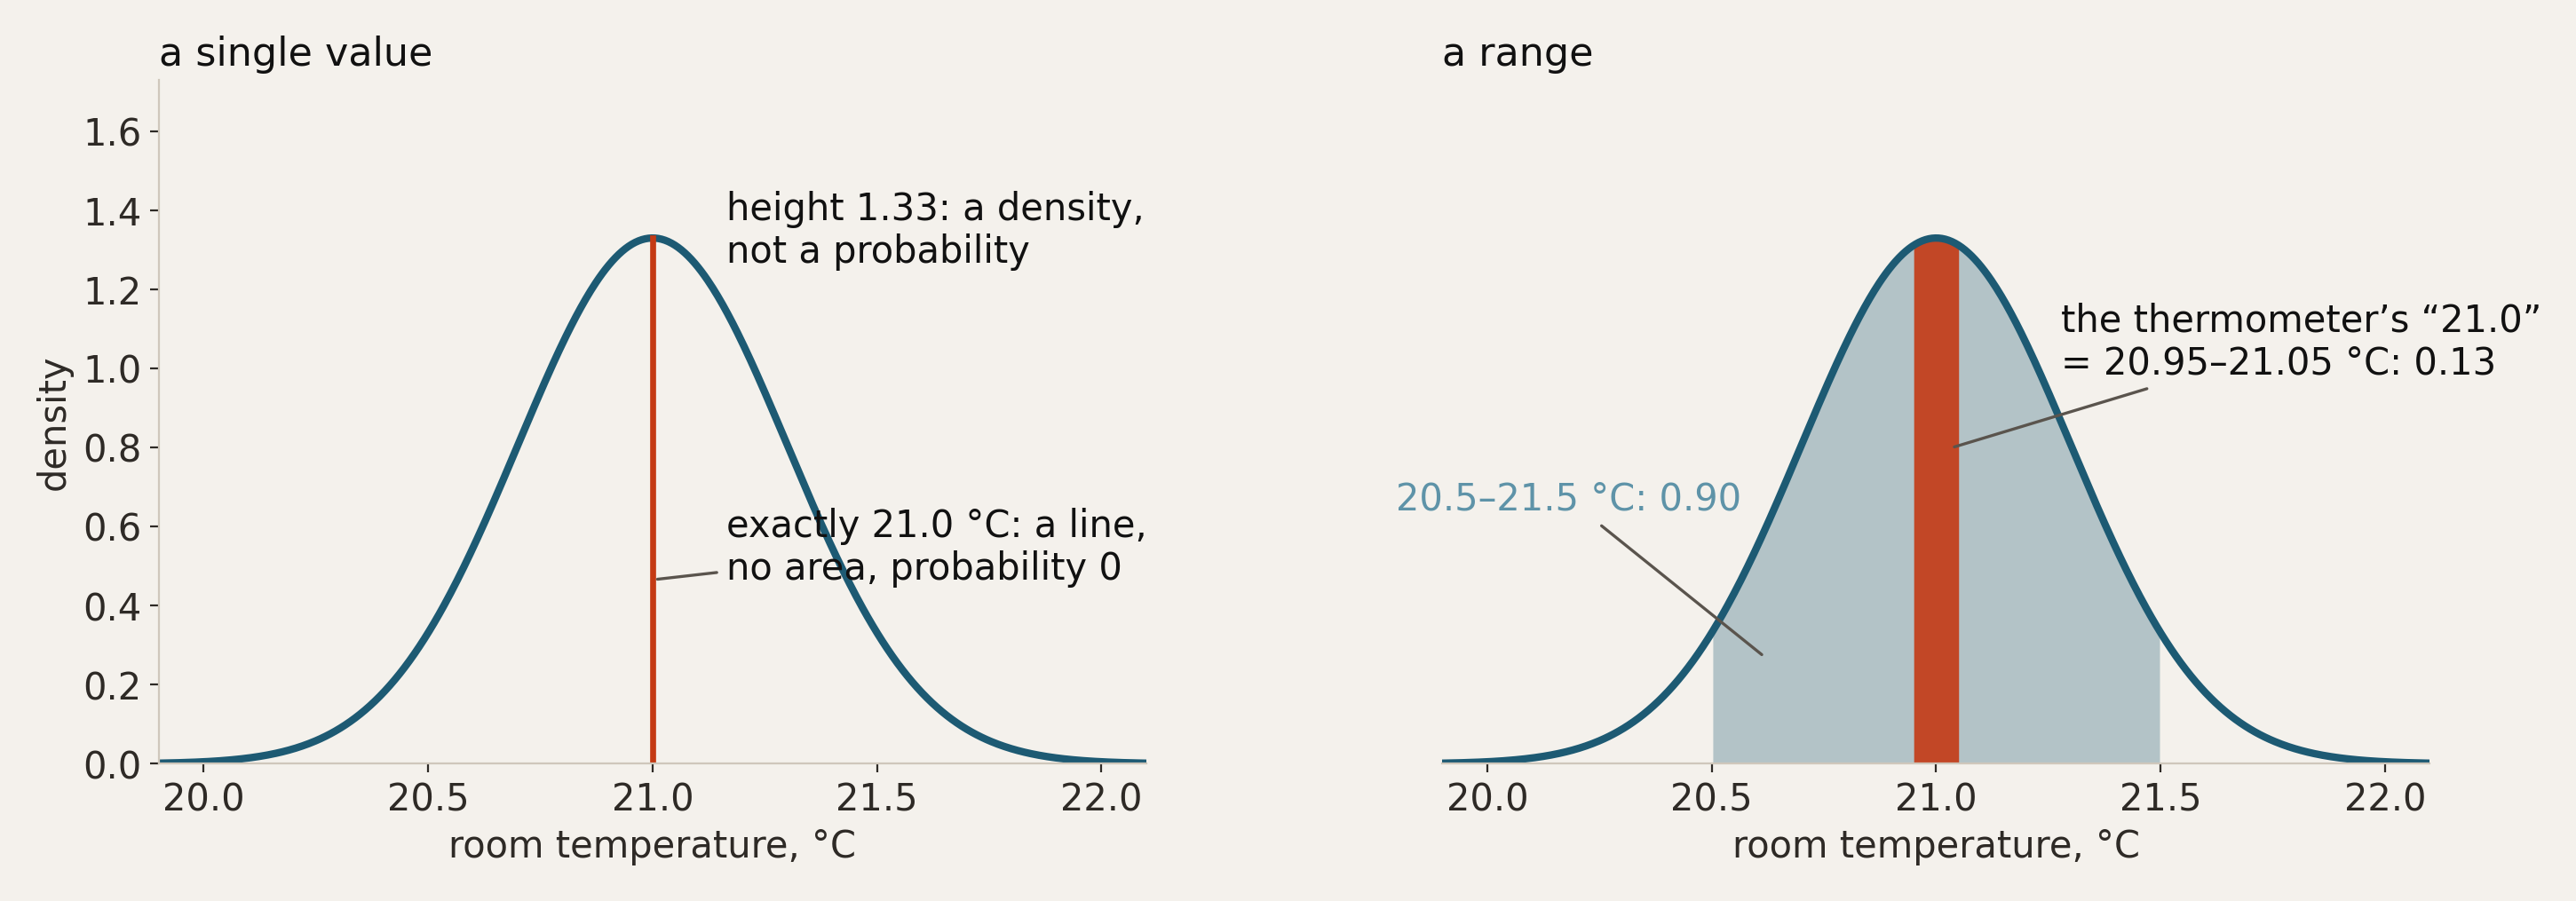
\includegraphics[width=0.9\textwidth]{lesson4/range.png}
\caption{Room temperature, mean 21\,°C, sd 0.3. Only an area under the curve is a probability.}
\label{fig:range}
\end{figure}

What you can ask about is a range. The probability that the temperature lies between $20.5$ and $21.5$ is the area under the curve between those two values, and here that area is $0.90$. Even the thermometer that shows ``21.0'' is giving you a range: it rounds, so ``21.0'' means somewhere between $20.95$ and $21.05$, which has probability $0.13$.

The height of the curve is therefore not a probability. It is a \emph{density}, and only an area under a density is a probability. The quickest way to convince yourself: at its peak, the curve in this example has height $1.33$, and no probability can be larger than one. This is why the y-axis of a continuous distribution should say \emph{density}. For a count, like a die or messages per day, single values do have a probability: those are bars.

\subsubsection{Same rolls, two plots: only one is a distribution}
Notice what is \emph{not} in the definition: whether you draw bars or a line. A plot is a distribution because it follows the three rules, not because of how it looks. The most common plot I get handed as ``the distribution'' is the result of \texttt{value\_counts} followed by a bar chart. Figure~\ref{fig:dice} shows why that is not the same thing. Ten rolls of a fair die happened to produce no 5 and no 6. The left plot silently drops those faces from the axis, and its counts only mean something if you know there were ten rolls. It describes ten rolls, not the die. The right plot puts every outcome the process \emph{can} produce on the x-axis, including the ones that didn't happen, and its y-axis holds shares that sum to one. Only that plot can be compared with a model (here $1/6$ per face) or with a second sample of a different size. Sometimes you really do want counts; then say so on the axis and don't call it a distribution.

\begin{figure}[H]
\centering
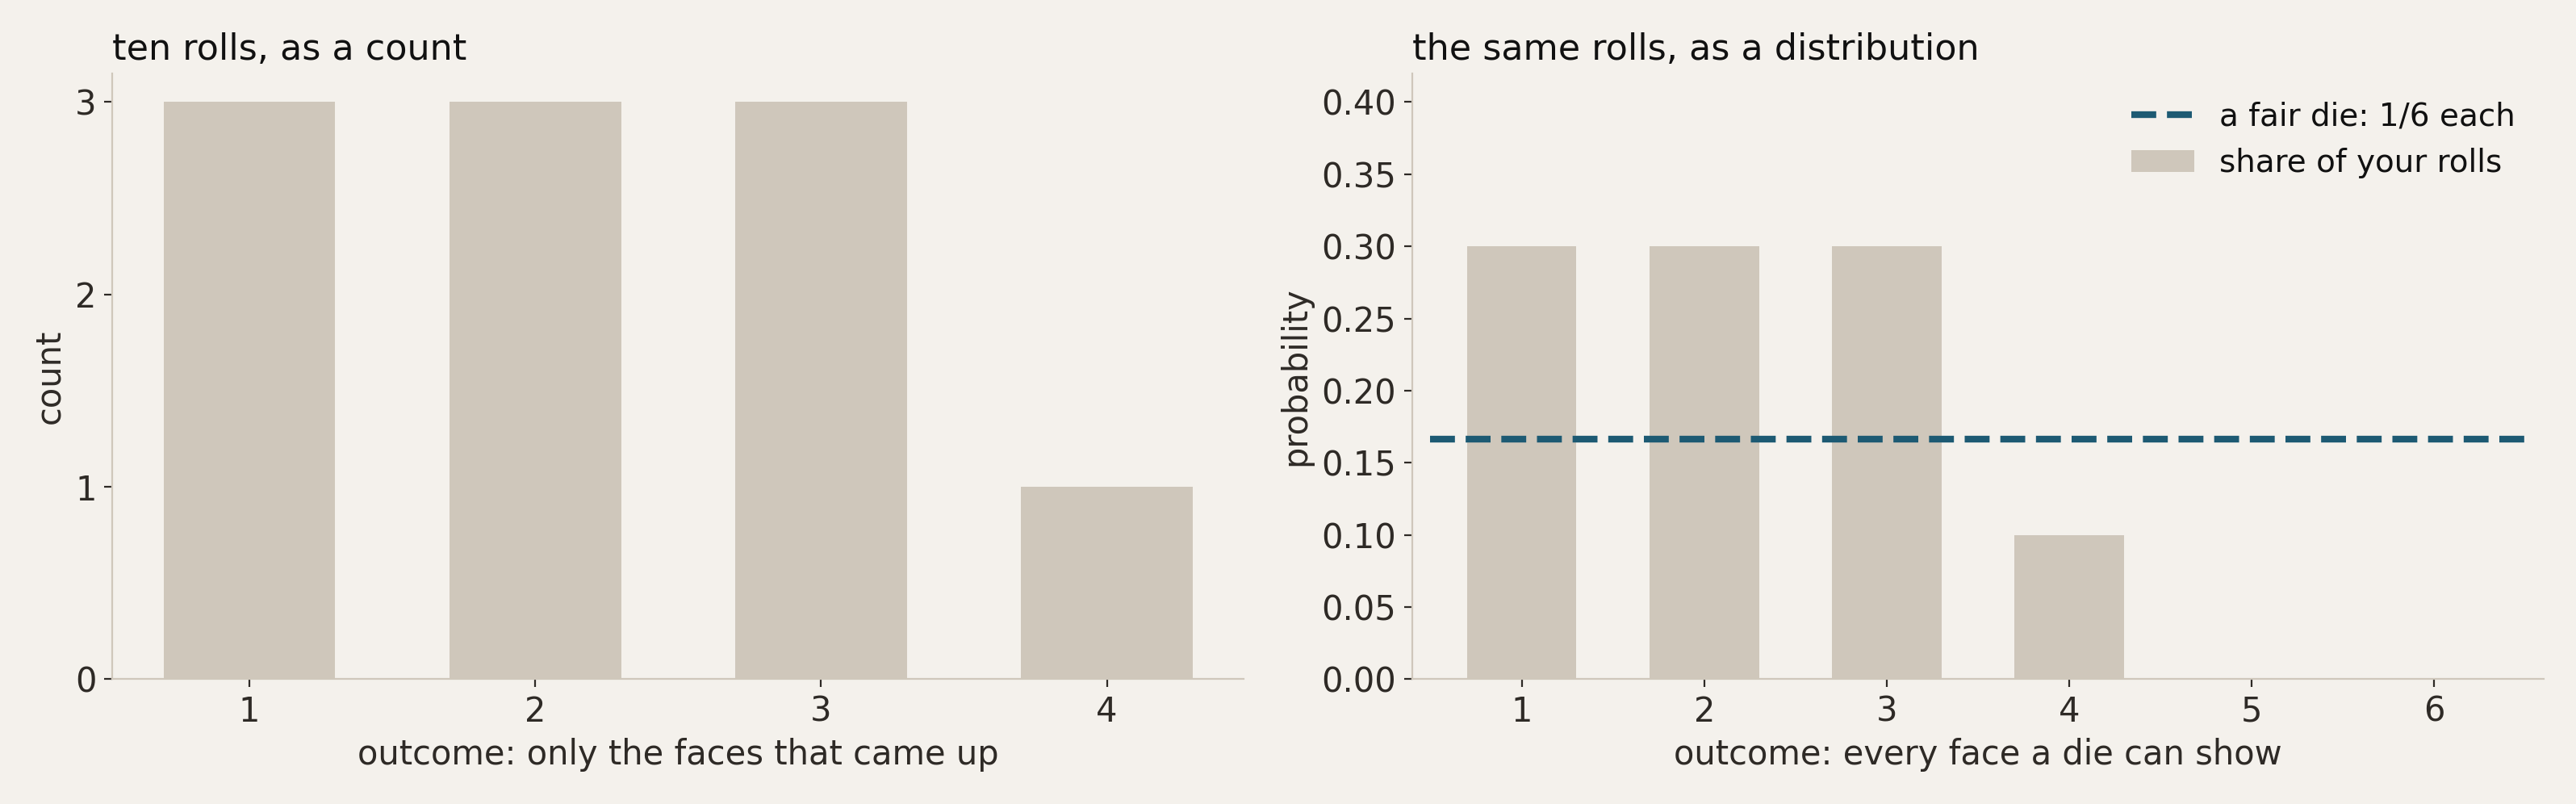
\includegraphics[width=\textwidth]{lesson4/dice.png}
\caption{The same ten rolls of a fair die, twice. Only the right plot is a distribution.}
\label{fig:dice}
\end{figure}

\subsubsection{Start from what you know about the process}
The skill I want you to practise is choosing a distribution by thinking about how your numbers came about, before you look at a histogram. Stand under a tree and count how many leaves fall in each minute. You cannot predict which leaf falls when, but you do know a few things about the process, and each of them narrows down the choice:

\begin{itemize}
\item \textbf{What kind of number is it?} A count: $0, 1, 2, 3, \ldots$ Never $-1$, never $2.5$. So we need a discrete family.
\item \textbf{Are the events independent?} Yes: one leaf doesn't pull another one down.
\item \textbf{Is the rate steady?} On a calm day, roughly: about the same number of leaves every minute, give or take chance.
\end{itemize}

Those three facts are exactly the assumptions of the \emph{Poisson} distribution, and then a single number, the average per minute, describes the whole distribution. The interesting part is what happens when an assumption breaks. When the wind picks up, the rate is no longer steady: gusts make it wander, and the counts spread out far more than a Poisson allows. Then you need another family. We will meet exactly this in chat data under question two.

\subsubsection{Six shapes, six ways numbers come about}
You don't need to memorise formulas for the families of distributions. What you need is the one-liner that tells you which process produces which shape. Table~\ref{tab:families} has the six we use in this course.

\begin{table}[H]
\centering
\begin{tabularx}{\textwidth}{@{}l X l@{}}
\toprule
\textbf{Family} & \textbf{The process that produces it} & \textbf{Example} \\
\midrule
Normal & Many small, independent parts \emph{added} up & Body height \\
Lognormal & Many factors \emph{multiplied} together & Duration of a project \\
Exponential & The wait for the next event, at a steady rate & Time between messages \\
Poisson & The number of events in a window, at a steady rate & Leaves per minute \\
Weibull & Time until something stops, when the risk changes with age & Lifetime of a part \\
Pareto & The rich get richer & Followers on social media \\
\bottomrule
\end{tabularx}
\caption{Six families and the processes behind them.}
\label{tab:families}
\end{table}

The assumption people forget is the steady rate. Poisson and exponential both need one. Put the arrivals at a station during rush hour and during a quiet afternoon in one column, and neither fits. Poisson is the only count in the table, so its bars are probabilities; the others are curves where an area is a probability.

\subsubsection{Adding makes a bell; multiplying makes a long tail}
The difference between the first two families is one of the most useful things you can know about data. Roll thirty dice and add them up. Each die on its own is flat: every face is equally likely. But the sum is a bell. Two dice already make a triangle, five look like a bell, thirty are a bell. Human height works the same way: it is the sum of the contributions of more than a hundred genes that control the length of your femur, your spine, your neck. Many small things added together: that is where the normal distribution comes from\footnote{This is the central limit theorem, without the formula.}.

Now multiply instead of add. Every factor makes the result more lopsided, with a long tail to the right. Projects work like this: a delay doesn't add a fixed week, it stretches everything that depends on it. If task $a$ takes $1.5$ times as long as planned and it has to be done ten times, the delay compounds. One trick is worth remembering here: the logarithm of a product is a sum of logarithms,
$$\log(x_1 \cdot x_2 \cdots x_n) = \log x_1 + \log x_2 + \cdots + \log x_n.$$
So if something is made by multiplying, its \emph{logarithm} is made by adding, and the logarithm looks like a bell. That is exactly what a lognormal distribution is.

\paragraph{Project planning: delays multiply.}
Figure~\ref{fig:sip} shows this in real data: 10,100 tasks from ten years of commercial software development, each with the estimated and the actual number of hours\footnote{The SiP dataset: Jones, D. \& Cullum, S. (2019), \url{https://github.com/Derek-Jones/SiP_dataset}, CC BY-NC-ND 4.0. Erik Bernhardsson analysed the same data in ``Why software projects take longer than you think'' (erikbern.com, 2019).}. The median task is exactly on time, so the estimates are not simply optimistic. But the tail runs one way. The average task takes $1.37$ times its estimate, one in ten takes more than twice as long, one in a hundred more than seven times, and the worst one $281$ times. A bell with this mean and standard deviation would put $39\%$ of the tasks below zero hours, which is impossible. On a log axis, though, the ratios form a rough bell around $1$: finishing in half the time ($13\%$) is about as common as taking twice as long ($10\%$). Symmetric in factors, not in hours. That is the signature of multiplying. (The spike in the middle is not the work but the people: $34\%$ of the tasks were booked at exactly their estimate.)

\begin{figure}[H]
\centering
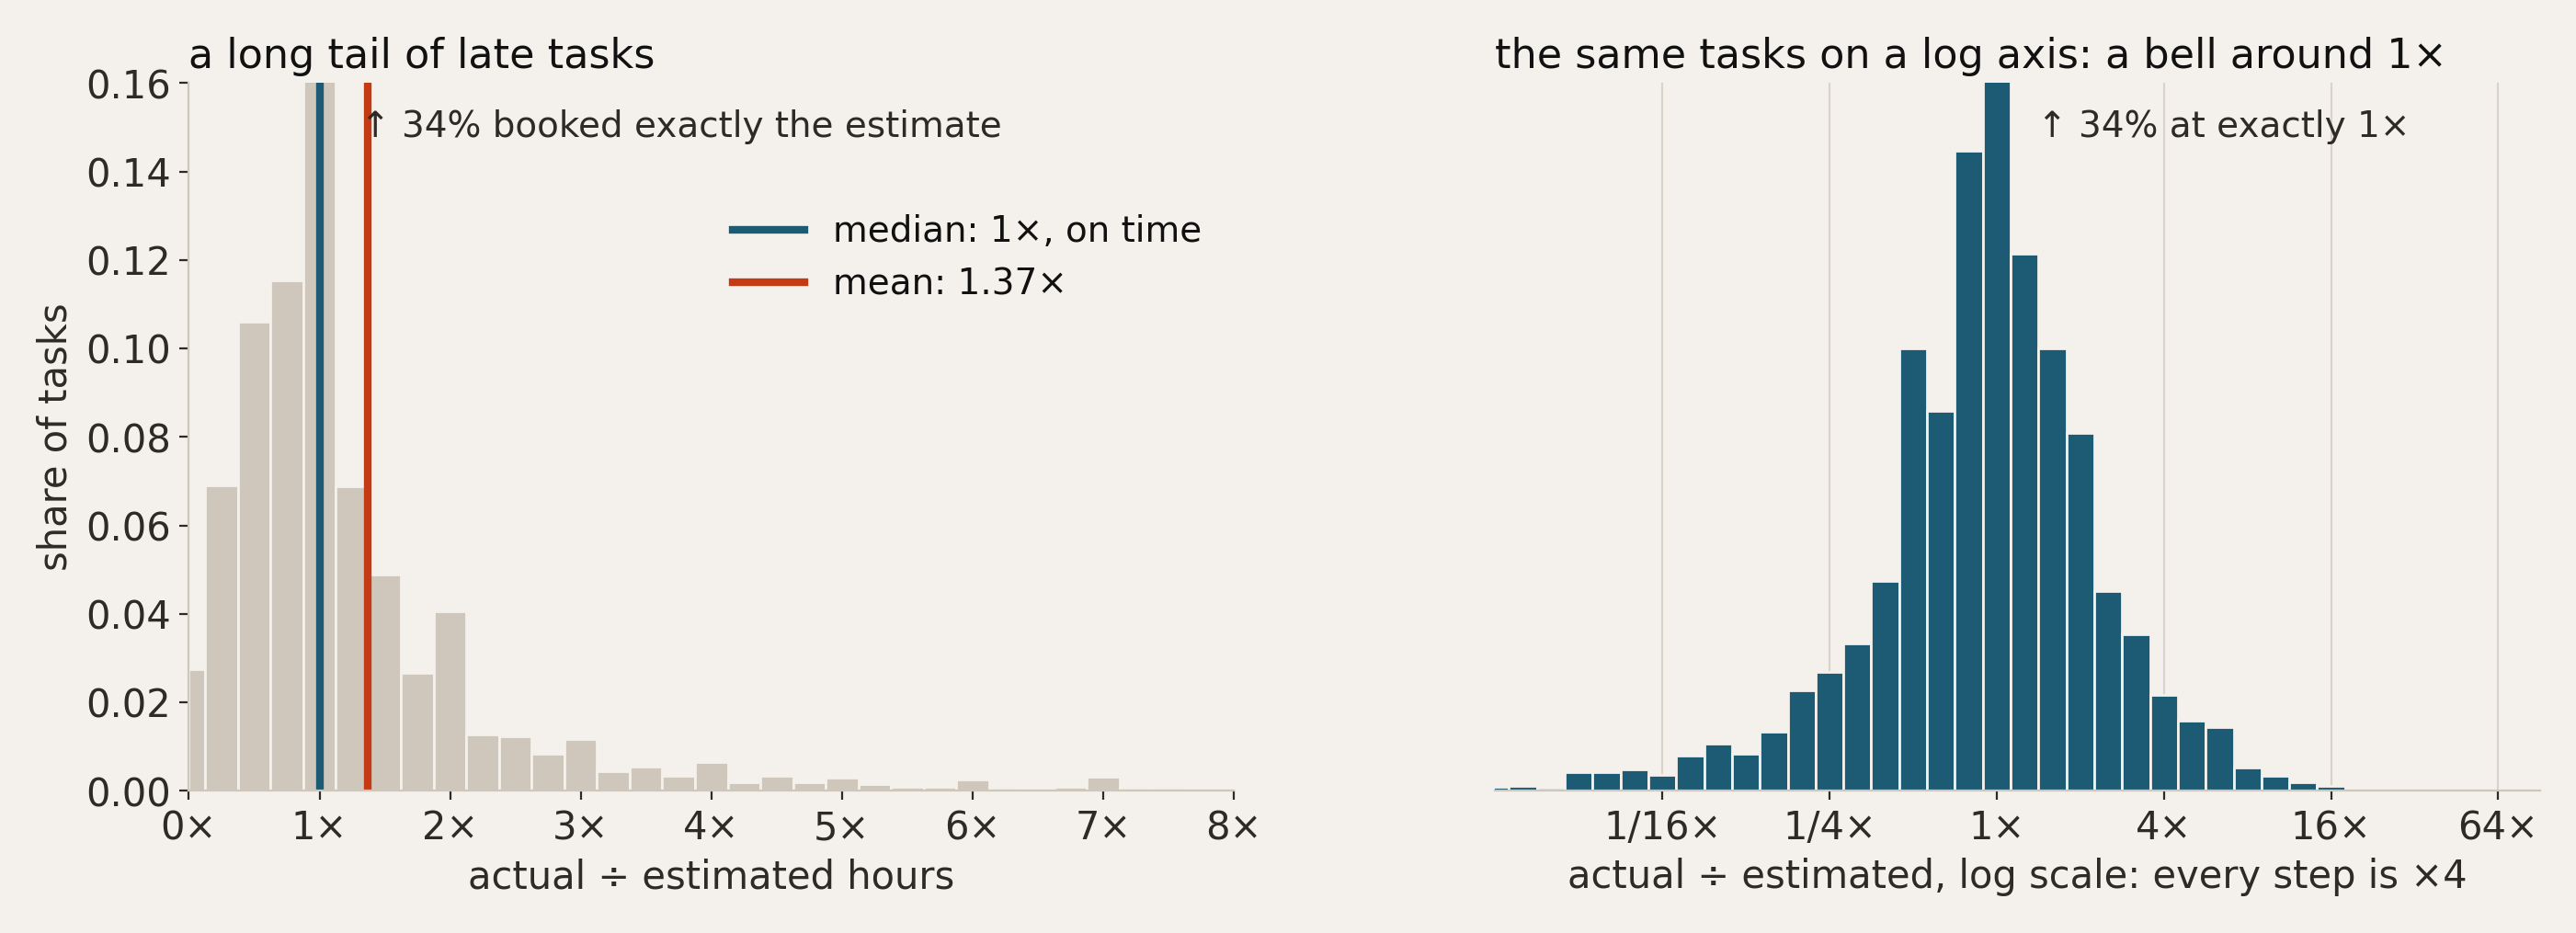
\includegraphics[width=0.8\textwidth]{lesson4/sip_tasks.png}
\caption{Actual divided by estimated hours for 10,100 software tasks. On a log axis the ratios form a rough bell around $1\times$.}
\label{fig:sip}
\end{figure}

\againconcretely
Dice add up to a bell. Project delays multiply into a long tail. Leaves on a calm day are a Poisson count. In each case the family followed from what we knew about how the numbers came about, not from a histogram. A distribution describes a random process: every possible outcome, with shares that sum to one. What you know about the process narrows down the family: a count or a measurement, added or multiplied, a steady rate or not. Then the data gets to check that choice. That is question two.

% ─────────────────────────────────────────────
\subsection{Which distribution fits my data?}
\label{sec:fitting}
A computer will fit any family to any data, and it will always return a winner. Choosing the family is your job. Fitting a distribution consists of three steps, and the order matters.

\begin{enumerate}
\item \textbf{Think.} Which families make sense for how these numbers came about? Is it a count or a measurement? Can it be negative? Is it a sum or a product, does it have a steady rate, does it have a snowball effect? Often several families fit about equally well; then the process decides.
\item \textbf{Fit.} For each family that makes sense, let the computer find the parameters under which your data is most probable: the mean and standard deviation of a bell, the rate of a Poisson. This is called \emph{maximum likelihood}, and it is the part computers are good at.
\item \textbf{Check.} Do model and data agree, up to the differences chance makes anyway? Look where they differ, in the tails too. A qq-plot shows you.
\end{enumerate}

The worst way to start is to hand a column to a fitter and report whatever wins. A winner that makes no sense for the process is noise, not an answer. The distribution fitter in goad, the course toolkit, also gives you test scores for every family. With thousands of rows every family gets rejected by a formal test, so use the scores to rank, and use your eyes and your knowledge of the process for the rest. A count is fitted with \texttt{discrete=True}, because a count has a probability per whole number.

\subsubsection{Messages per day: the rate isn't steady}
Messages per day on a chat channel are a count, so the first candidate is a Poisson. Before fitting, check its assumption: is the rate steady? On a chat channel that is unlikely, and figure~\ref{fig:irc} shows how unlikely. Over 250 ordinary Thursdays the Italian Ubuntu channel had between $10$ and almost $1{,}800$ messages a day, $564$ on average. A Poisson with that mean allows about $24$ messages either way and squeezes $164$ of the $250$ days into a single bar. Clearly wrong.

\begin{figure}[H]
\centering
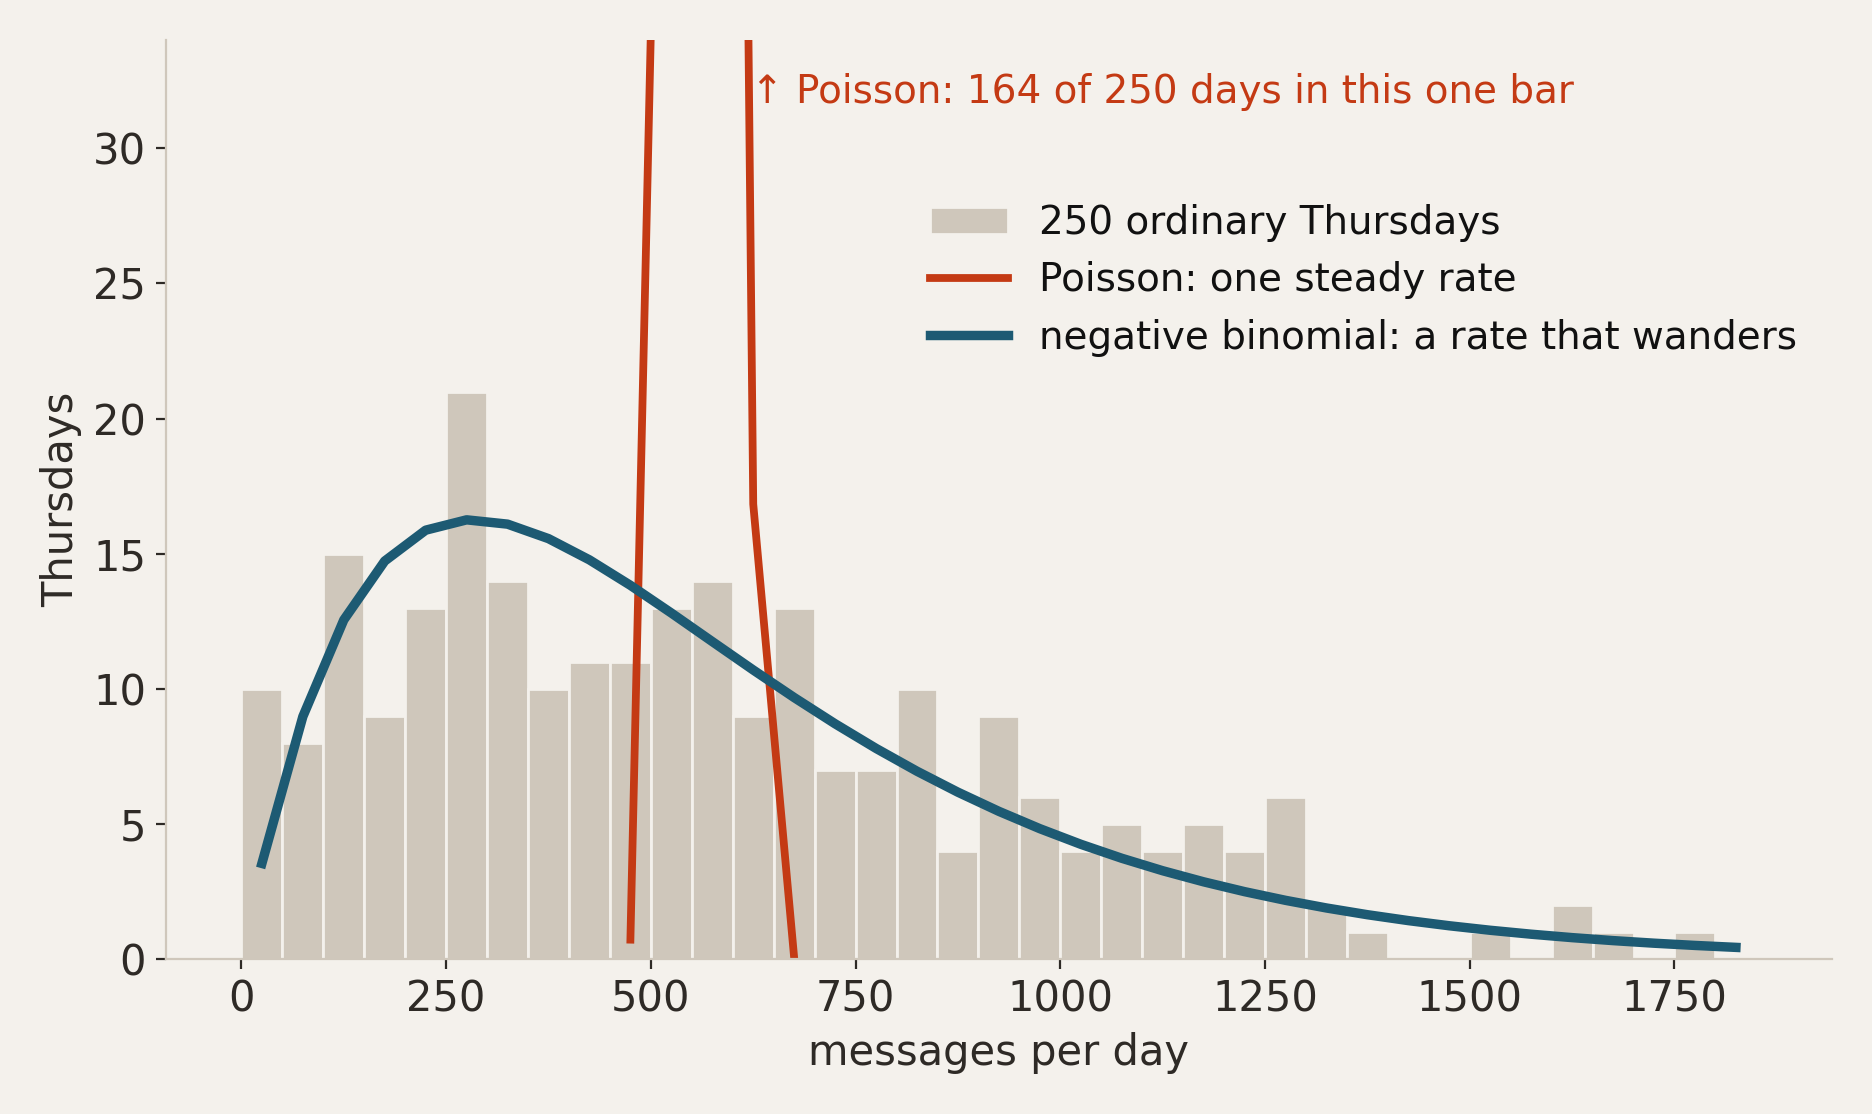
\includegraphics[width=0.65\textwidth]{lesson4/irc_poisson.png}
\caption{Messages per ordinary Thursday in \#ubuntu-it. Poisson (red) against negative binomial (blue).}
\label{fig:irc}
\end{figure}

There is a quick way to see this without a plot. For a Poisson distribution, the variance equals the mean:
$$\Var(X) = \E[X].$$
If the variance of your counts is much larger than their mean, the Poisson is the wrong model. The \emph{negative binomial} is a Poisson whose rate is itself drawn anew every day, and it fits these data well: mean $564$, standard deviation $399$. Who is around, what broke, the time of year: they all move the rate. That is the wind from the leaves example.

Notice that the failed Poisson is informative. It tells you the rate moves. The honest summary of an ordinary Thursday is not ``about 560 messages'' but ``a rate of about 560 that routinely halves or doubles''.

\subsubsection{A strange best fit can mean several groups}
The penguin dataset\footnote{Palmer Penguins: Horst, A.M., Hill, A.P. \& Gorman, K.B. (2020), \url{https://allisonhorst.github.io/palmerpenguins/}.} contains the flipper length of 333 birds. Put that column into a fitter and the best single curve is a \emph{beta} distribution. A beta describes a percentage you are unsure about: flip a coin ten times, get seven heads, and the beta tells you which values of ``the chance of heads'' are plausible. It lives between zero and one. The fitting library (scipy) lets every family shift and stretch, so it can lay a beta over $170$ to $235$ millimetres. The fit is real; the meaning is nil. Nothing about a flipper length is a percentage.

\begin{figure}[H]
\centering
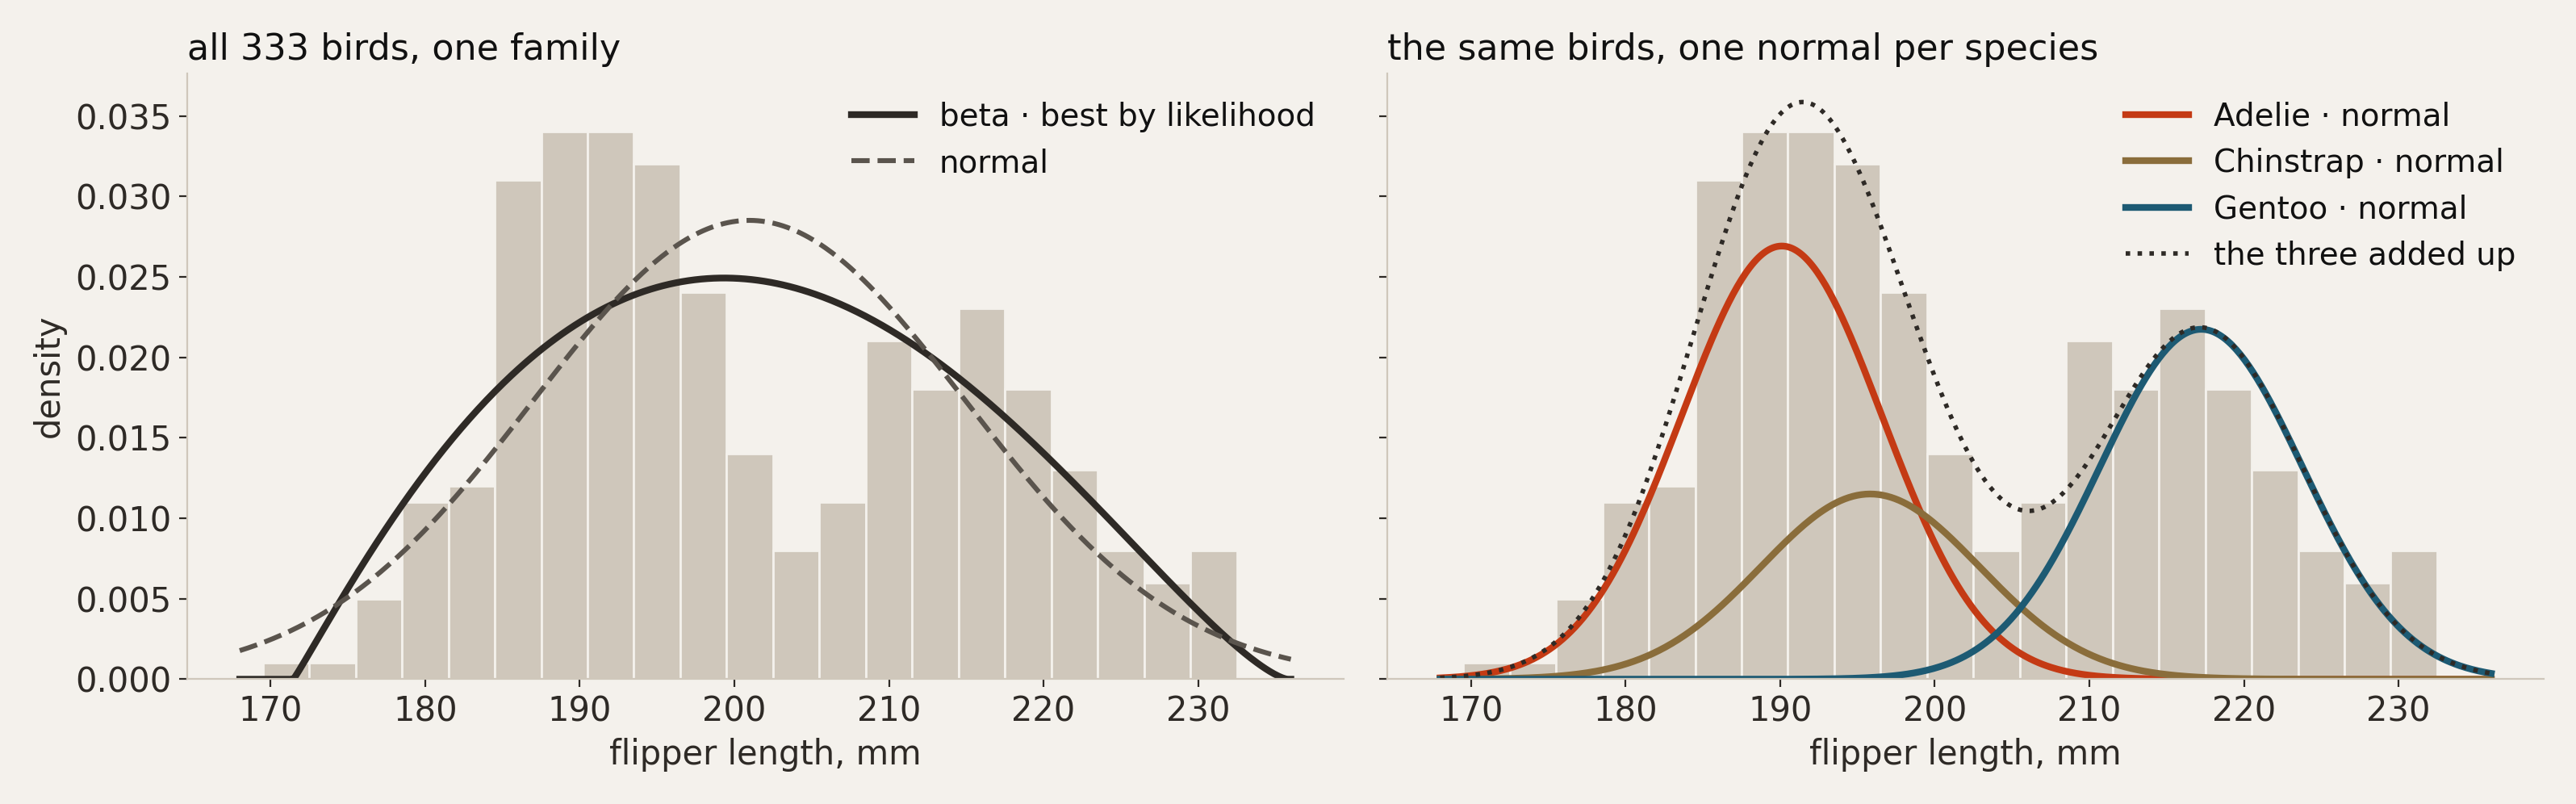
\includegraphics[width=\textwidth]{lesson4/penguins_split.png}
\caption{Left: one curve for all 333 penguins. Right: one normal distribution per species.}
\label{fig:penguins}
\end{figure}

A winner like that is a warning. The histogram has two humps, and two humps usually mean two or more groups. Here we know the groups: three species. Fit one normal distribution per species and each one fits fine (figure~\ref{fig:penguins}); Adelie and Chinstrap overlap, Gentoo sits twenty millimetres further. The column was never one population. A species has a flipper length; ``a penguin'' doesn't. What told us to split was knowing the data, not the fit table. With some experience you can also see it in the plot: the gap between the humps is about two standard deviations, which is what two bells lying next to each other look like.

\subsubsection{A qq-plot shows where model and data disagree}
You know the boxplot. Its box marks three quantiles: the lengths below which a quarter, a half and three quarters of the birds fall. A \emph{qq-plot} does that for every single observation. Sort the data; for each rank, ask the fitted model which value it expects at that rank; plot the real value against the expected value. If the model is right, the dots lie on the diagonal. Where the dots leave the line, the model is wrong, and the way they leave it usually tells you why.

\begin{figure}[H]
\centering
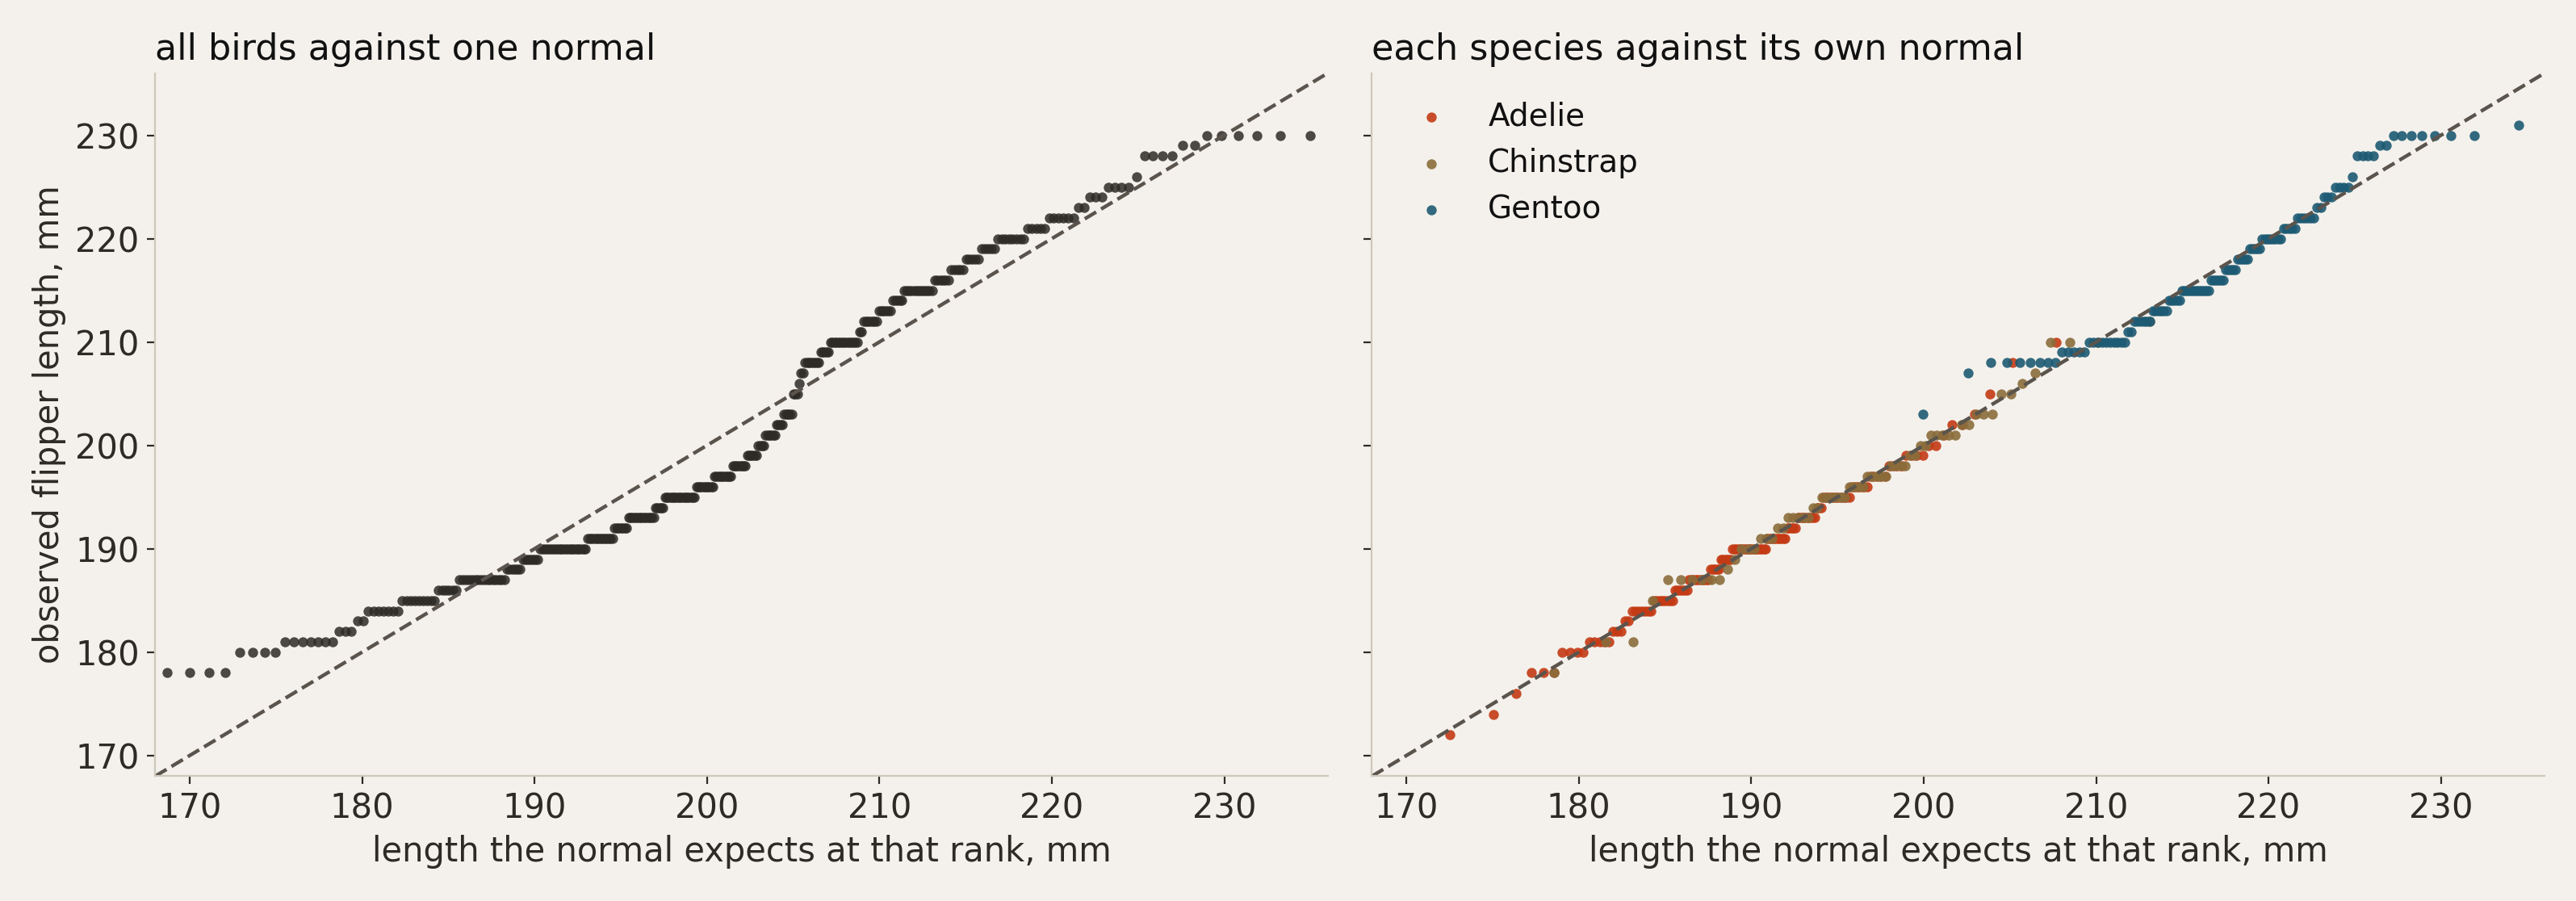
\includegraphics[width=\textwidth]{lesson4/penguins_qq.png}
\caption{qq-plots against the normal. Left: all birds against one bell. Right: each species against its own.}
\label{fig:penguins-qq}
\end{figure}

For all penguins against one bell, the dots snake around the line in an S-shape: too few birds in the middle, too many at both ends, because the pooled data has a dip in the middle where a bell has its peak. Each species against its own bell follows the line, apart from small steps that come from measuring to the whole millimetre. The qq-plot is most useful in the tails, where a histogram has too few points to show you anything. We use it on taxi fares under question three.

\againconcretely
The fitter crowned a stretched beta. Split by species, and three plain bells appear. The fitter always returns a winner; whether that winner makes sense is your call. Before trying a stranger family, ask whether your column holds several groups. Then check with a qq-plot: where the dots leave the line, the model is wrong. Messages per day failed the Poisson because the rate moves; the penguins failed one bell because there were three populations. Both failures told us something about the data.

% ─────────────────────────────────────────────
\subsection{What is an outlier?}
\label{sec:outliers}
Here is the central idea of this question: \emph{an outlier is not a property of the data, it is a property of your model.} An outlier is a value your model didn't expect. Pick the wrong model, and ordinary values look strange.

\subsubsection{What does an outlier mean?}
When you find an outlier, there are three possible explanations, and I list them in the order in which you should suspect them.

\begin{enumerate}
\item \textbf{A wrong model.} This is by far the most common reason, certainly among students. The value is ordinary; your distribution doesn't fit the data, or it mixes groups. A value that looks like an outlier may simply belong in a different distribution: another species of penguin, another phase of a process. Fix the model, not the data.
\item \textbf{A rare, real value.} Unusual but possible: sometimes there really is an extremely long taxi ride or an exceptionally busy day. Keep it; it is often the most interesting row in your dataset.
\item \textbf{An error.} A value the process cannot produce: a negative duration, a date in 1970, an amount of 70 million among amounts of 4,000. Remove it, and say that you did. But consider this last, not first.
\end{enumerate}

Statistics can point at the rows to look at. Which of the three it is takes knowledge of the process. And the two rules of thumb everyone knows, the boxplot whiskers and ``more than three standard deviations from the mean'', both assume a bell. On skewed data, they flag ordinary values.

\subsubsection{The bell has no room for expensive rides}
Taxi fares, $6{,}433$ New York rides. The mean is \$13, the median \$9.50: the tail pulls the mean up. Read the qq-plot in figure~\ref{fig:taxi-qq} the same way as the penguins: each dot is one ride, its real fare against the fare the model expects at that rank. Against a fitted bell the dots bend away from the line. At the bottom the bell expects negative fares; at the top it expects about \$55 where the real top is \$150. A right-skewed family, the lognormal, follows much further.

\begin{figure}[H]
\centering
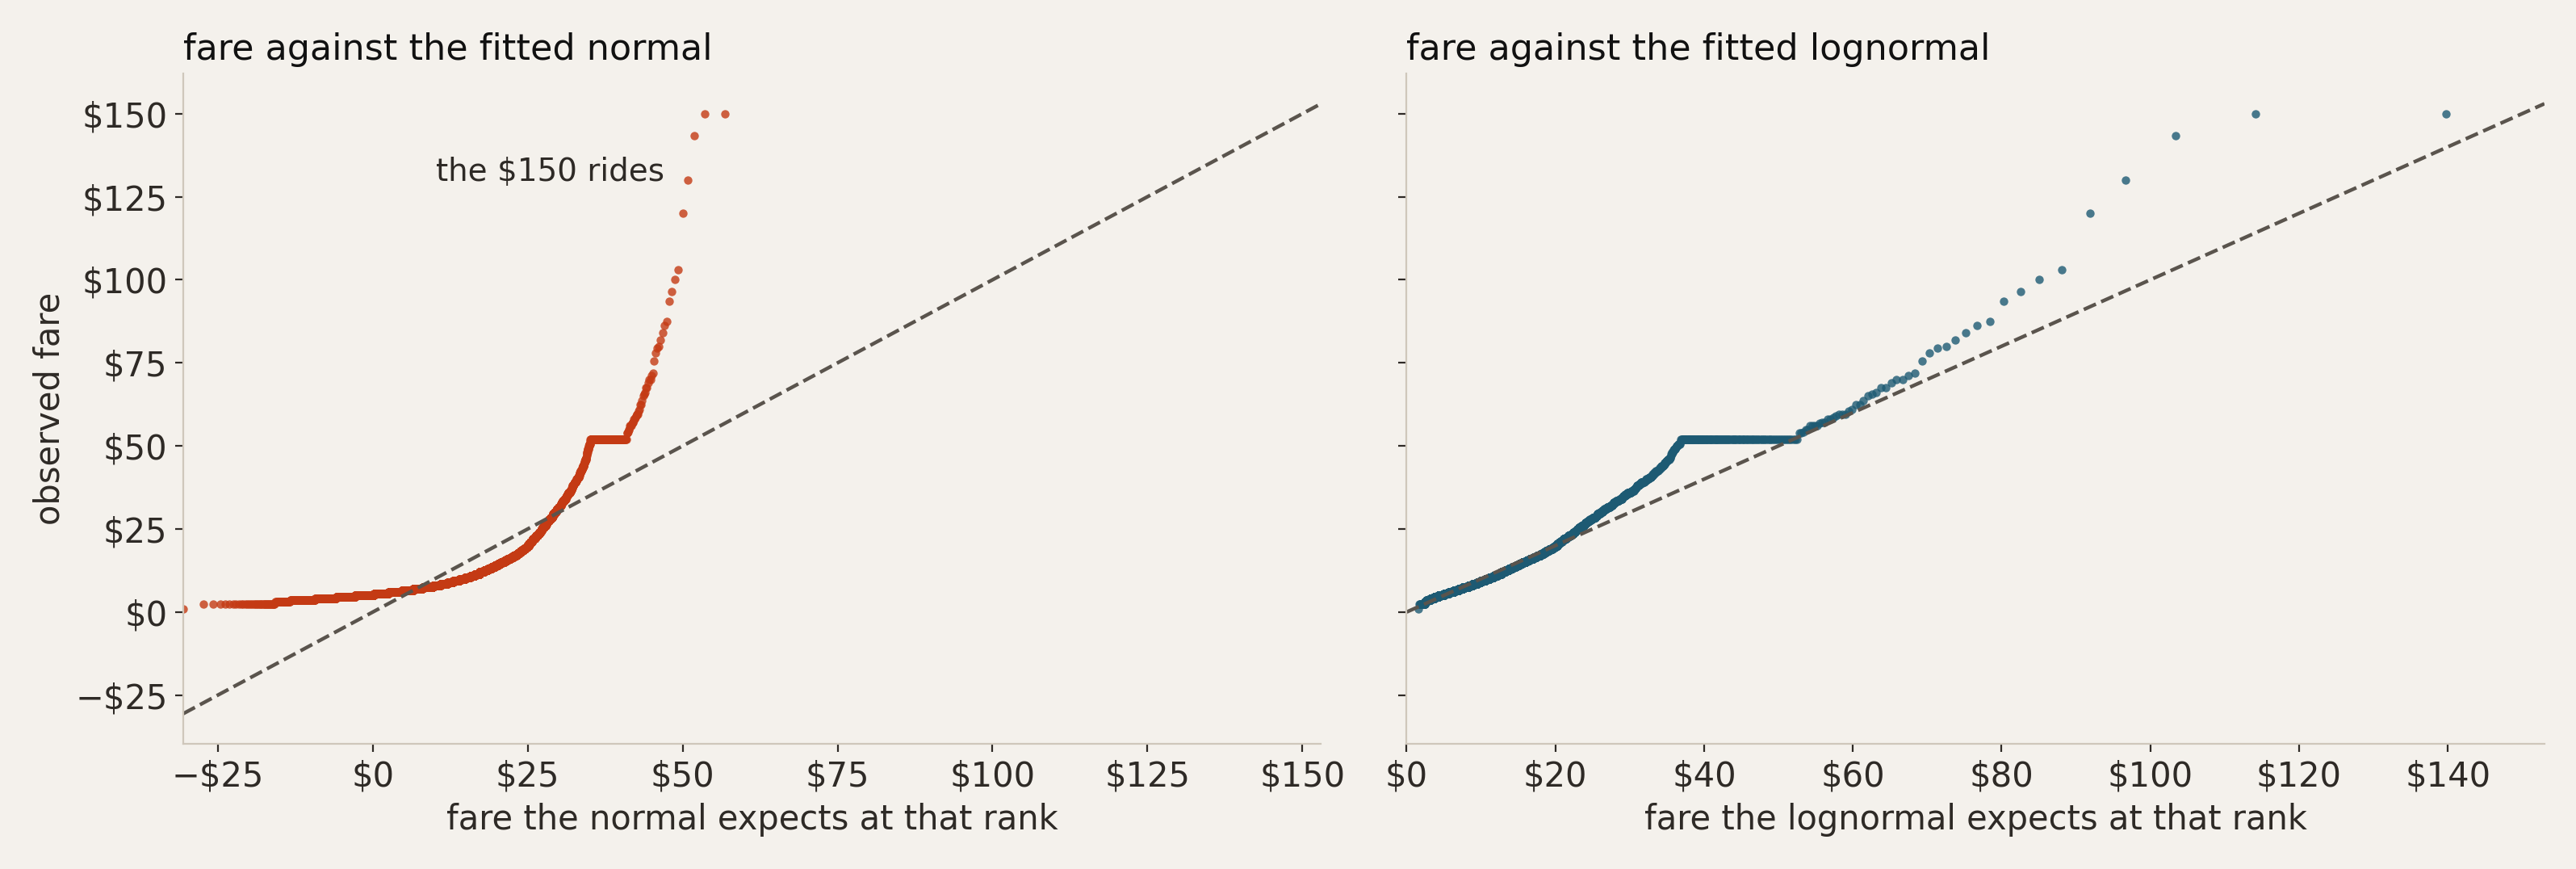
\includegraphics[width=\textwidth]{lesson4/taxi_qq.png}
\caption{Taxi fares against a bell (left) and a lognormal (right).}
\label{fig:taxi-qq}
\end{figure}

Why are the fares so skewed? Don't read a deep mechanism into it. Fares are a base charge plus a meter, so mostly a sum; the skew comes from the trips. Most rides are short, and for long distances people choose a train or a car, because a taxi becomes too expensive. The tail is cut off by people's choices, not by chance. We just need a family with room on the right. And the flat run at \$52 is the fixed airport fare: a second process in the same column.

\subsubsection{Outliers, or the wrong model?}
Most people use an outlier definition without knowing they chose one. The dots beyond the whiskers of a boxplot come from Tukey's rule: the whiskers reach $1.5$ times the interquartile range (IQR) past the box, and everything beyond is drawn as an outlier. Tukey designed that rule for roughly bell-shaped data; on a normal distribution it flags $0.7\%$ of the observations.

\begin{figure}[H]
\centering
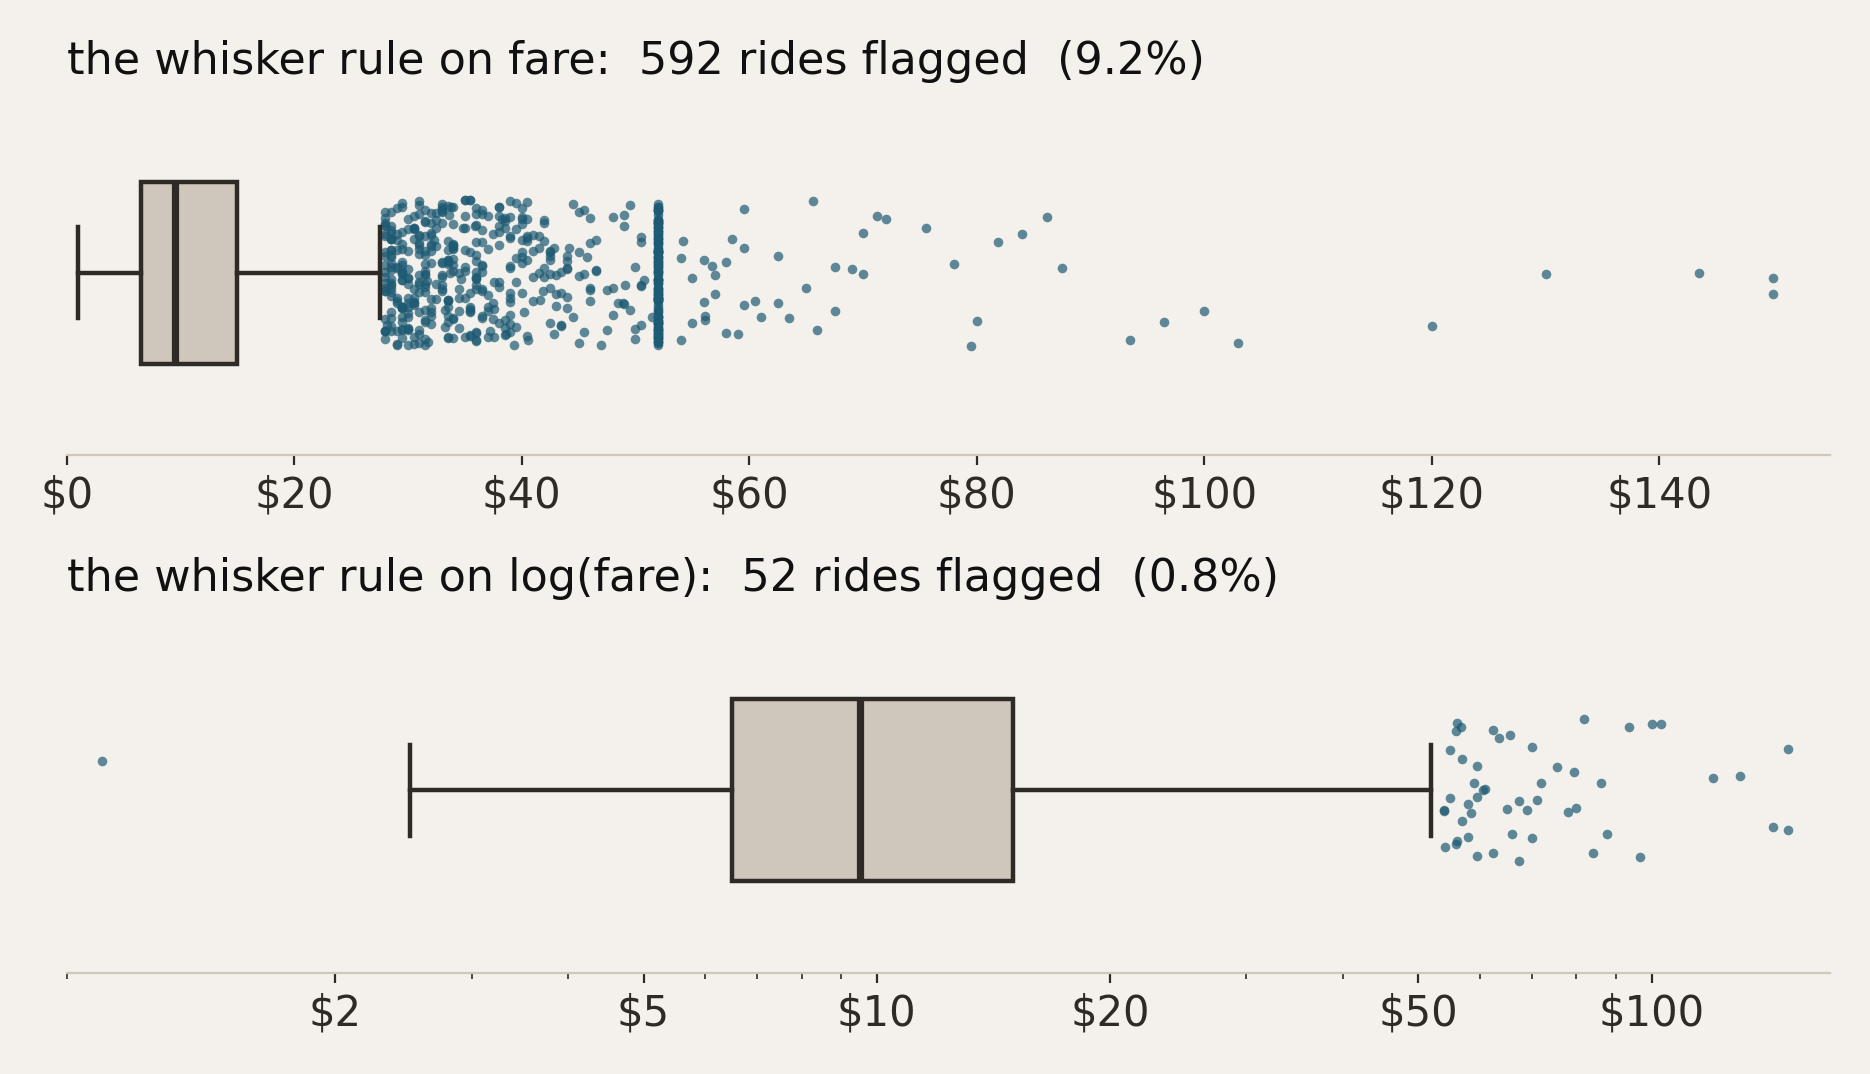
\includegraphics[width=0.65\textwidth]{lesson4/taxi_whiskers.png}
\caption{Tukey's whisker rule on the taxi fares, and on the logarithm of the same fares.}
\label{fig:whiskers}
\end{figure}

On the taxi fares, Tukey's rule flags $592$ rides as outliers: $9.2\%$, including every airport ride (figure~\ref{fig:whiskers}). Not $592$ strange rides: nothing is wrong with those rides, the model behind the rule is. Apply the same rule to the \emph{logarithm} of the fare, whose shape is close to a bell, and it flags $52$ rides, $0.8\%$, which is about what the rule expects. The rule isn't wrong. It assumes a bell.

\subsubsection{The whisker rule makes four assumptions}
Tukey's rule quietly makes four assumptions:

\begin{enumerate}
\item \textbf{Shape: roughly symmetric.} A bell, not a long tail. On taxi fares the rule flags 592 ordinary rides.
\item \textbf{Population: one group.} Mix groups, and an ordinary member of another group looks like an outlier.
\item \textbf{Numbers: continuous.} Measurements. Counts, categories and rounded values pile up on the same numbers, and the quartiles and whiskers land on awkward ties.
\item \textbf{Order: independent.} Every value stands on its own. In a time series, where every value builds on the previous one, the rule is out of scope.
\end{enumerate}

Break one of these, and a dot past the whiskers no longer means ``unusual''. The same four assumptions hide behind ``more than three standard deviations''. Next: an analysis that breaks three of them.

\subsubsection{What not to do: judge data without the process}
Here is a real student analysis from an earlier year, shown as an example of what not to do. The data is the axle load of a garbage truck over a morning. The student saw gaps and an uneven number of measurements per day, wrote that this suggested ``inconsistent data collection'', and concluded that about $30\%$ of the data was unreliable.

\begin{figure}[H]
\centering
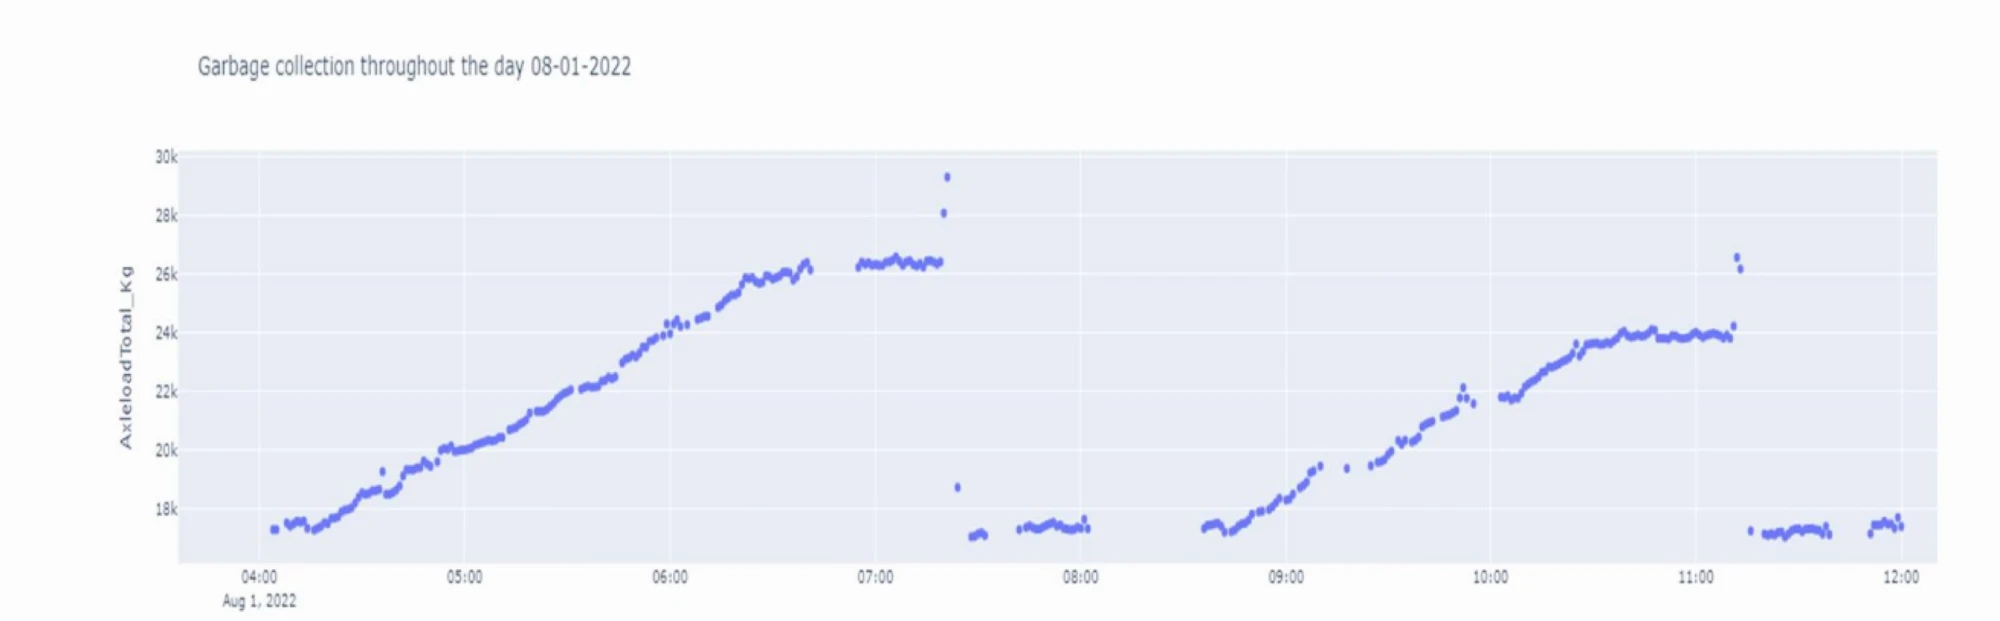
\includegraphics[width=\textwidth]{lesson4/garbage_truck.png}
\caption{The axle load of a garbage truck through one morning.}
\label{fig:garbage}
\end{figure}

Now think about the process instead. The load grows while the truck collects along its route. It drops back to roughly the weight of the empty truck when the truck is emptied, and then the next round starts. The flat stretches and the gaps fit driving to the dump, waiting and breaks. A sudden drop of several thousand kilos is not someone throwing out a very heavy bag; it is the truck being unloaded. And a day with fewer measurements might simply be a shorter round.

Check the four assumptions, and three of them are broken. The measurements are not independent: if the truck weighs $20{,}000$ kg and two bags are added, the next measurement is $20{,}050$ kg, strongly correlated with the previous one. There is not one population: a full truck and an empty truck are different situations. And so there is no single distribution over the day, and no whisker rule or threshold can say anything about reliability. None of this data was shown to be unreliable; the analysis never asked how it was made.

What would work? Two things, both suggested by students in class: split the data into the two processes (collecting and unloading), and take the \emph{difference} between consecutive measurements. The differences ($10$ kg, $50$ kg, $100$ kg) are close to independent, and they do have a distribution. Against that distribution, a jump of $2{,}000$ kg during collection really is an outlier, and a very interesting one.

\subsubsection{One \$150 ride, three verdicts}
The most expensive ride in the dataset costs \$150. Is it an outlier? That depends entirely on the model you hold it against. Figure~\ref{fig:taxitail} shows, on a log scale, the share of rides at least this expensive: each step down is 1,000 times rarer. Black is the data.

\begin{figure}[H]
\centering
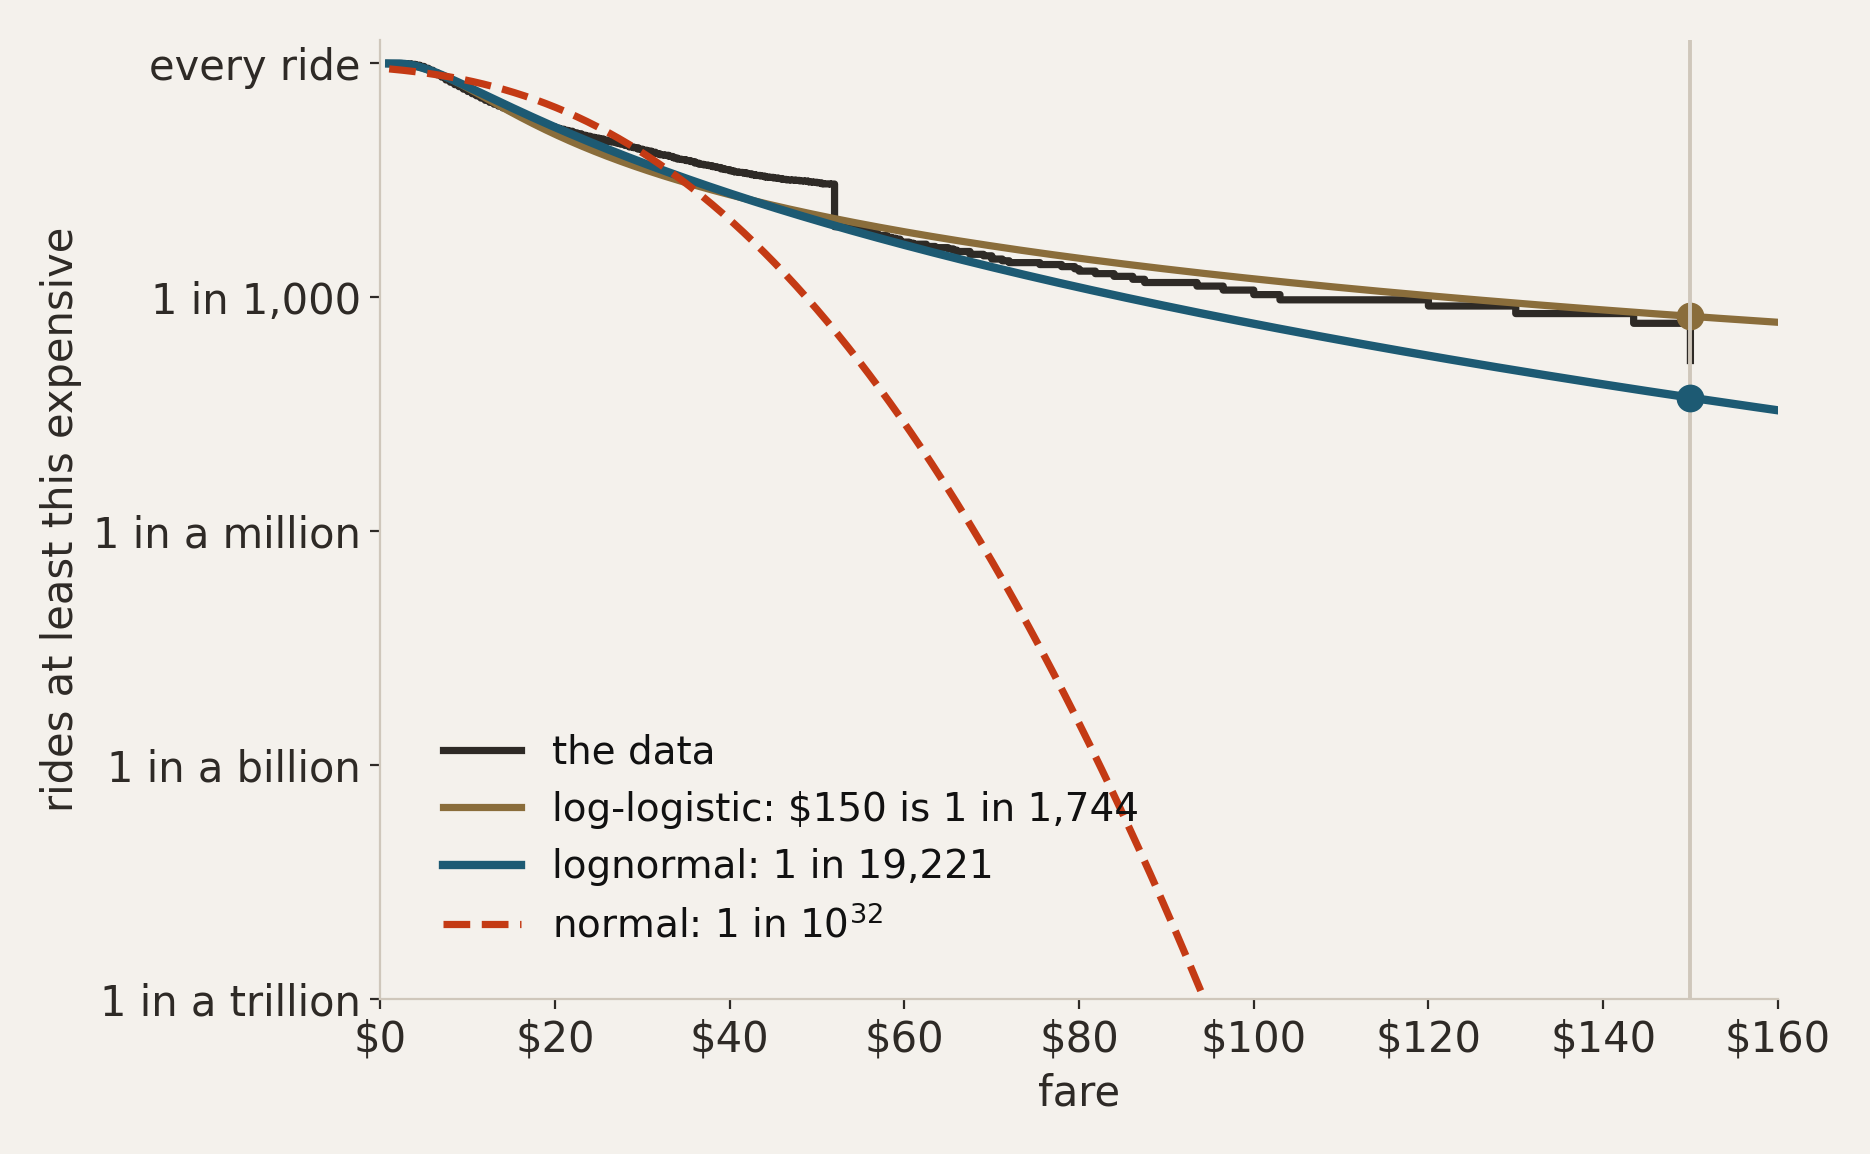
\includegraphics[width=0.65\textwidth]{lesson4/taxi_tail.png}
\caption{The share of rides at least this expensive, under three families.}
\label{fig:taxitail}
\end{figure}

\begin{itemize}
\item \textbf{1 in $10^{32}$.} Under a fitted bell the ride is $11.9$ standard deviations above the mean. To give you a feeling for that number: there are roughly $2 \times 10^{16}$ ants on earth\footnote{Schultheiss, P. et al. (2022). The abundance, biomass, and distribution of ants on Earth. \textit{PNAS}, 119(40).}. Pick a random ant; now I pick a random ant too, and it is the same one. Now do that twice in a row. That is the kind of rare we are talking about. Under this model, the ride cannot have happened.
\item \textbf{1 in 19,000.} Under the lognormal, the best of goad's families.
\item \textbf{1 in 1,700.} Under the log-logistic, a skewed family outside goad's list, which follows the real tail more closely. With $6{,}433$ rides, a few rides like this are within expectation.
\end{itemize}

The family decides how rare a value is. A check in numbers: $7$ rides cost \$100 or more; the lognormal expects $3$, the log-logistic $11$. And a warning: the Burr family has a better likelihood than both, because it fits the bulk of the data, and it expects $32$ rides of \$150 or more where there are $2$. The best fit overall is not the best fit in the tail, and the tail is where outlier questions live. Where data is thin, check the tail itself. Note that neither skewed family says ``delete the ride''; only the bell says it is impossible.

\subsubsection{Ordinary among all penguins, rare among her own}
A wrong model doesn't only make you find outliers that aren't there; it also makes you miss the ones that are. One Adelie female in the penguin data has a flipper of $202$ mm. Among all penguins she is completely ordinary: she stands in the middle of the crowd of another species, and no rule would flag her. Among the $73$ Adelie females she is two and a half standard deviations long, about one in $95$.

\begin{figure}[H]
\centering
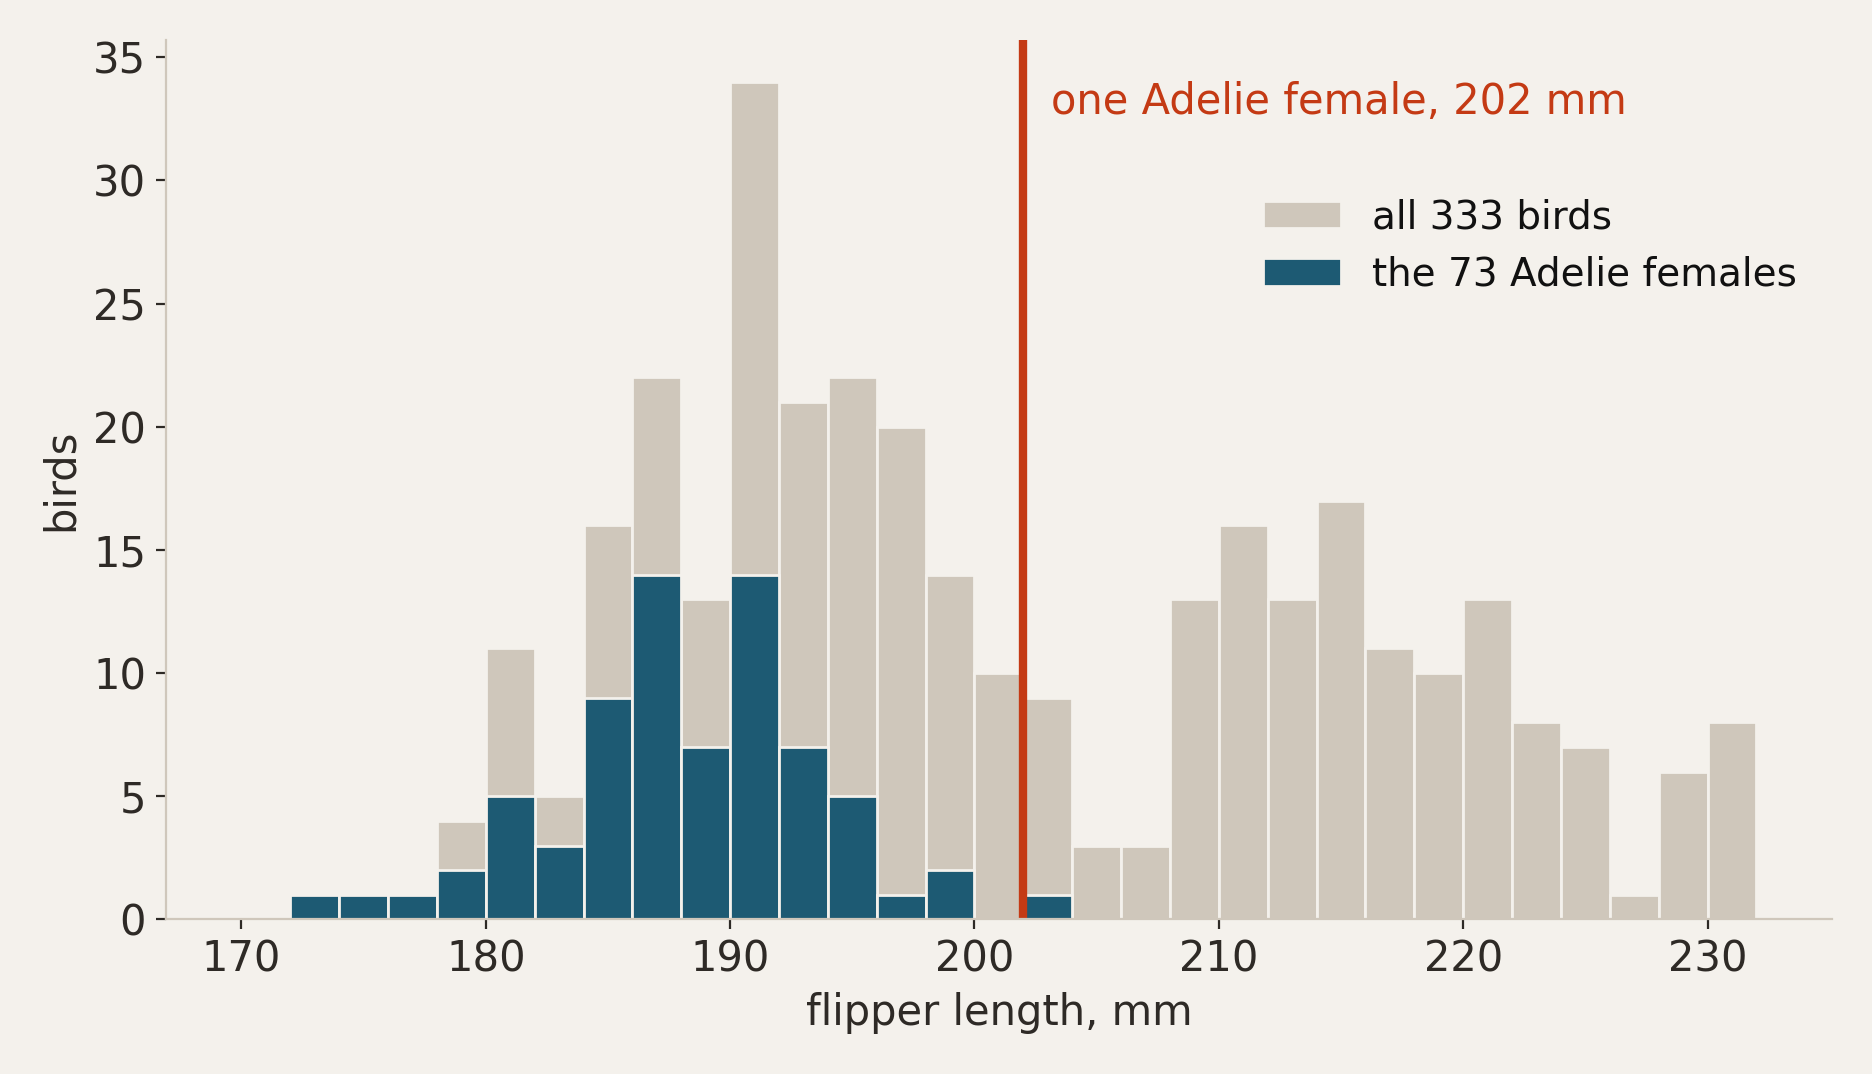
\includegraphics[width=0.65\textwidth]{lesson4/penguin_adelie.png}
\caption{Grey: all 333 birds. Blue: the 73 Adelie females. Red: one Adelie female with a 202 mm flipper.}
\label{fig:adelie}
\end{figure}

It runs the other way too: the longest flipper in the data, $231$ mm, looks rare among all penguins (one in $146$) and is an ordinary large Gentoo male (one in $22$). ``Unusual'' always means unusual \emph{for a population}, so pick a population that exists. What to do with her is something the numbers cannot settle. It could be a mistyped measurement, a bird whose sex or species was recorded wrongly, or a genuinely large female. Someone who handled the birds knows.

\paragraph{Why you want to find outliers.}
After all these warnings you might think outliers are a nuisance. They are not. Outliers are often the first sign of a problem: in a factory, an unusual measurement is often an early warning that something is about to break; in a sales process, it can announce a dissatisfied customer or rising costs. And outliers are a way into discovering \emph{groups} you didn't know about. In a chat export, for example, you will often find a sharp peak in message length around eight characters. That is not a habit of the writers: it is the export writing a placeholder such as ``image omitted'' every time someone sent a picture. It is a different process in the same column, and it does not belong in the distribution of what people write. Often, when you go looking for an outlier, what you are really looking for is a different process. That is why it pays to have more than the normal distribution in your toolbox.

\againconcretely
A \$150 taxi ride is impossible under a bell and merely rare under a skewed family. Same ride, different model. Before you call something an outlier, check that your distribution fits, in the tails too, and that it describes one population. If it fits and the value is still extreme: is it an error, or a rare real event? That takes knowledge of the process, not statistics. In your chat that might be an export glitch, a birthday, or the week someone joined. If you remove anything, report how many values, on what criterion, and whether your conclusion survives with them left in.

% ─────────────────────────────────────────────
\subsection{Did something change, or is it chance?}
\label{sec:change}
A distribution describes a process. When something changes the process, the distribution moves with it. Someone \emph{falls in love} and sends more messages, at different hours, to one person. A \emph{holiday} means fewer messages and a different rhythm of the day. A \emph{new release} fills a chat channel with questions. So you compare the distribution before and after the event.

The catch is that two samples always differ a little, even when they come from exactly the same process, and our eyes are very good at seeing change in noise. The question is therefore never ``is there a difference?'', but ``is the difference bigger than the differences chance alone produces?''

\subsubsection{Did this person's texting change?}
The example comes from the first chapter of \textit{Bayesian Methods for Hackers}\footnote{Davidson-Pilon, C. (2015). \textit{Bayesian Methods for Hackers: Probabilistic Programming and Bayesian Inference}. Addison-Wesley. The notebooks are at \url{https://github.com/CamDavidsonPilon/Probabilistic-Programming-and-Bayesian-Methods-for-Hackers}.}: the number of text messages one person sent per day, over $74$ days. From around day $45$ the average goes up from $17.8$ to $22.8$ messages a day. Did this person's texting habits change? Perhaps something happened: a new relationship, a new job. But look at the individual days: $2$ messages one day, $72$ another. With noise this large, a difference of $5$ a day could easily be luck. How do you tell?

\begin{figure}[H]
\centering
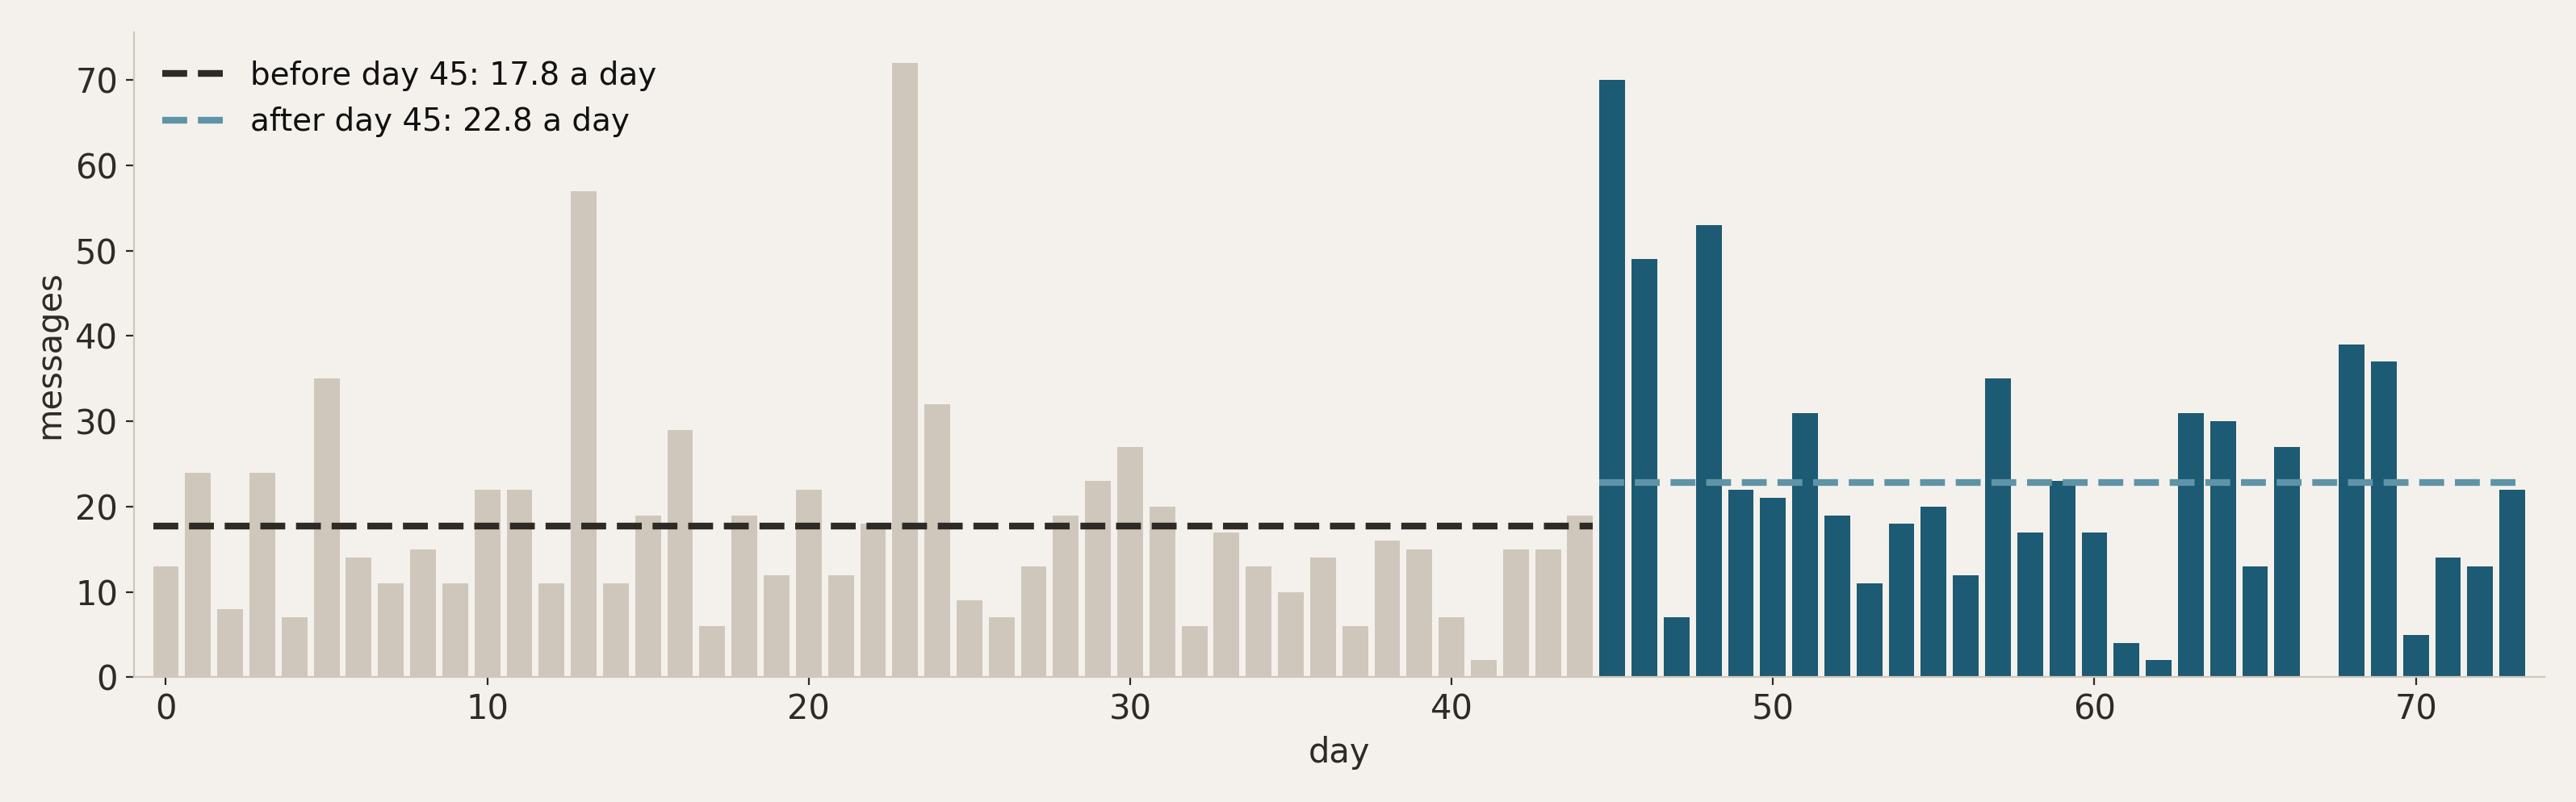
\includegraphics[width=\textwidth]{lesson4/texting.png}
\caption{Messages per day for 74 days.}
\label{fig:texting}
\end{figure}

\subsubsection{Shuffle the labels to see what chance does}
Here is a way to find out that needs no formula and no distribution family at all. If nothing changed at day $45$, then which days we call ``before'' and which ``after'' is arbitrary. So we can shuffle those labels.

\begin{definition}
\label{def:shuffle}
A \emph{shuffle test} (or permutation test) compares the difference between two groups with the differences you get when the group labels are randomly reassigned. Shuffle the labels, compute the difference again, and repeat many times (say $10{,}000$). The share of shuffles that produce a difference at least as large as the real one is the \emph{p-value}: how often chance alone does this well.
\end{definition}

For the texting data we keep $45$ days labelled ``before'' and $29$ labelled ``after'', shuffle, and compute the difference in means, ten thousand times. That cloud is what chance alone makes (figure~\ref{fig:texting-null}). The real difference sits in its upper tail, but $14\%$ of the shuffles produce a difference at least as large, in either direction ($p = 0.14$). A change is possible; this alone doesn't show it. Roughly: the more noise in your data, the larger the chance that what you see is chance.

\begin{figure}[H]
\centering
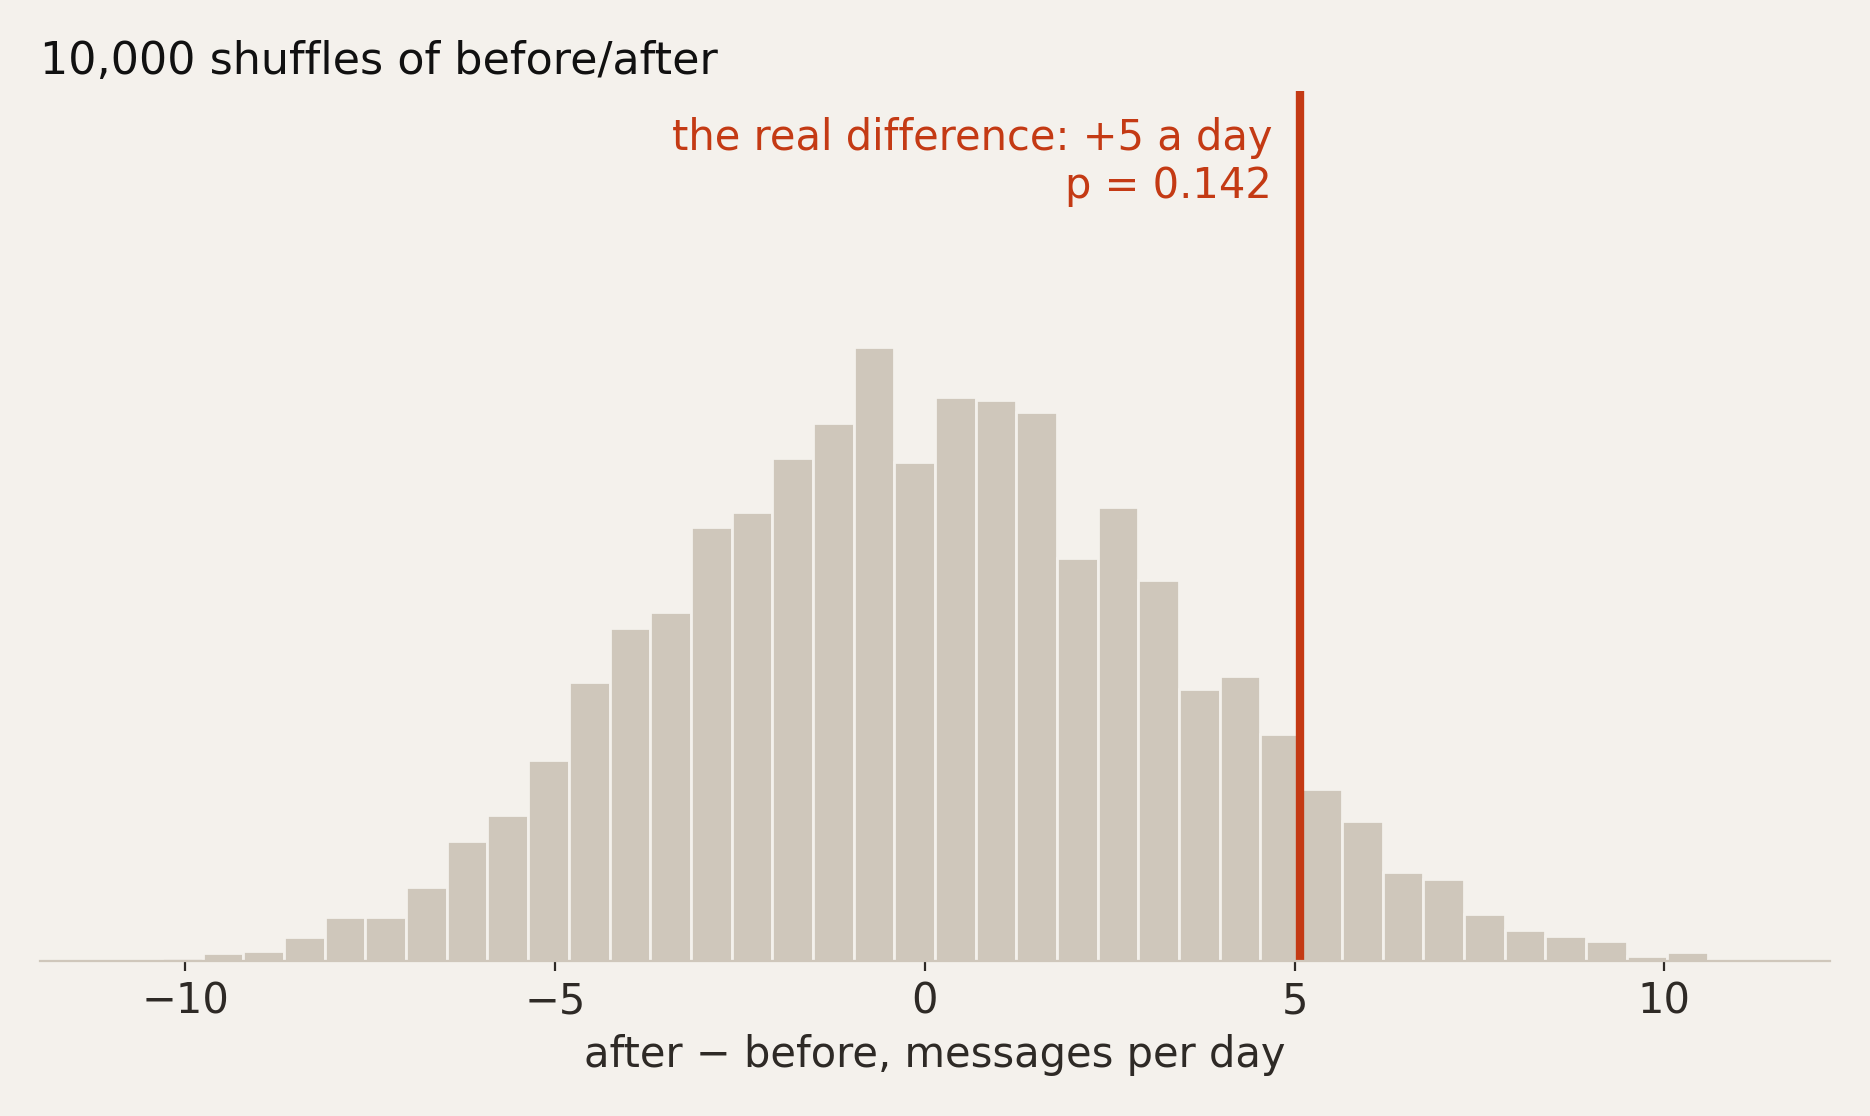
\includegraphics[width=0.65\textwidth]{lesson4/texting_null.png}
\caption{Grey: the differences chance produces in 10,000 shuffles. Red: the real difference, $+5$ a day.}
\label{fig:texting-null}
\end{figure}

\subsubsection{Bayesian Methods for Hackers: a confident switch}
The book answers the same question in a Bayesian way, and comes out much more confident. Its model says: the messages on each day are Poisson distributed, with rate $\lambda_1$ before an unknown day $\tau$ and rate $\lambda_2$ from $\tau$ on. The switch day $\tau$ gets a uniform prior: before we look at the data, every one of the $74$ days is equally likely to be the switch. A sampling method, Markov chain Monte Carlo (MCMC), then finds which combinations of $\lambda_1$, $\lambda_2$ and $\tau$ explain the data well. The verdict: from $17.8$ to $22.7$ messages a day, from day $44$ or $45$ on, and the probability that the rate went up is
$$P(\lambda_2 > \lambda_1) = 0.998.$$

\begin{figure}[H]
\centering
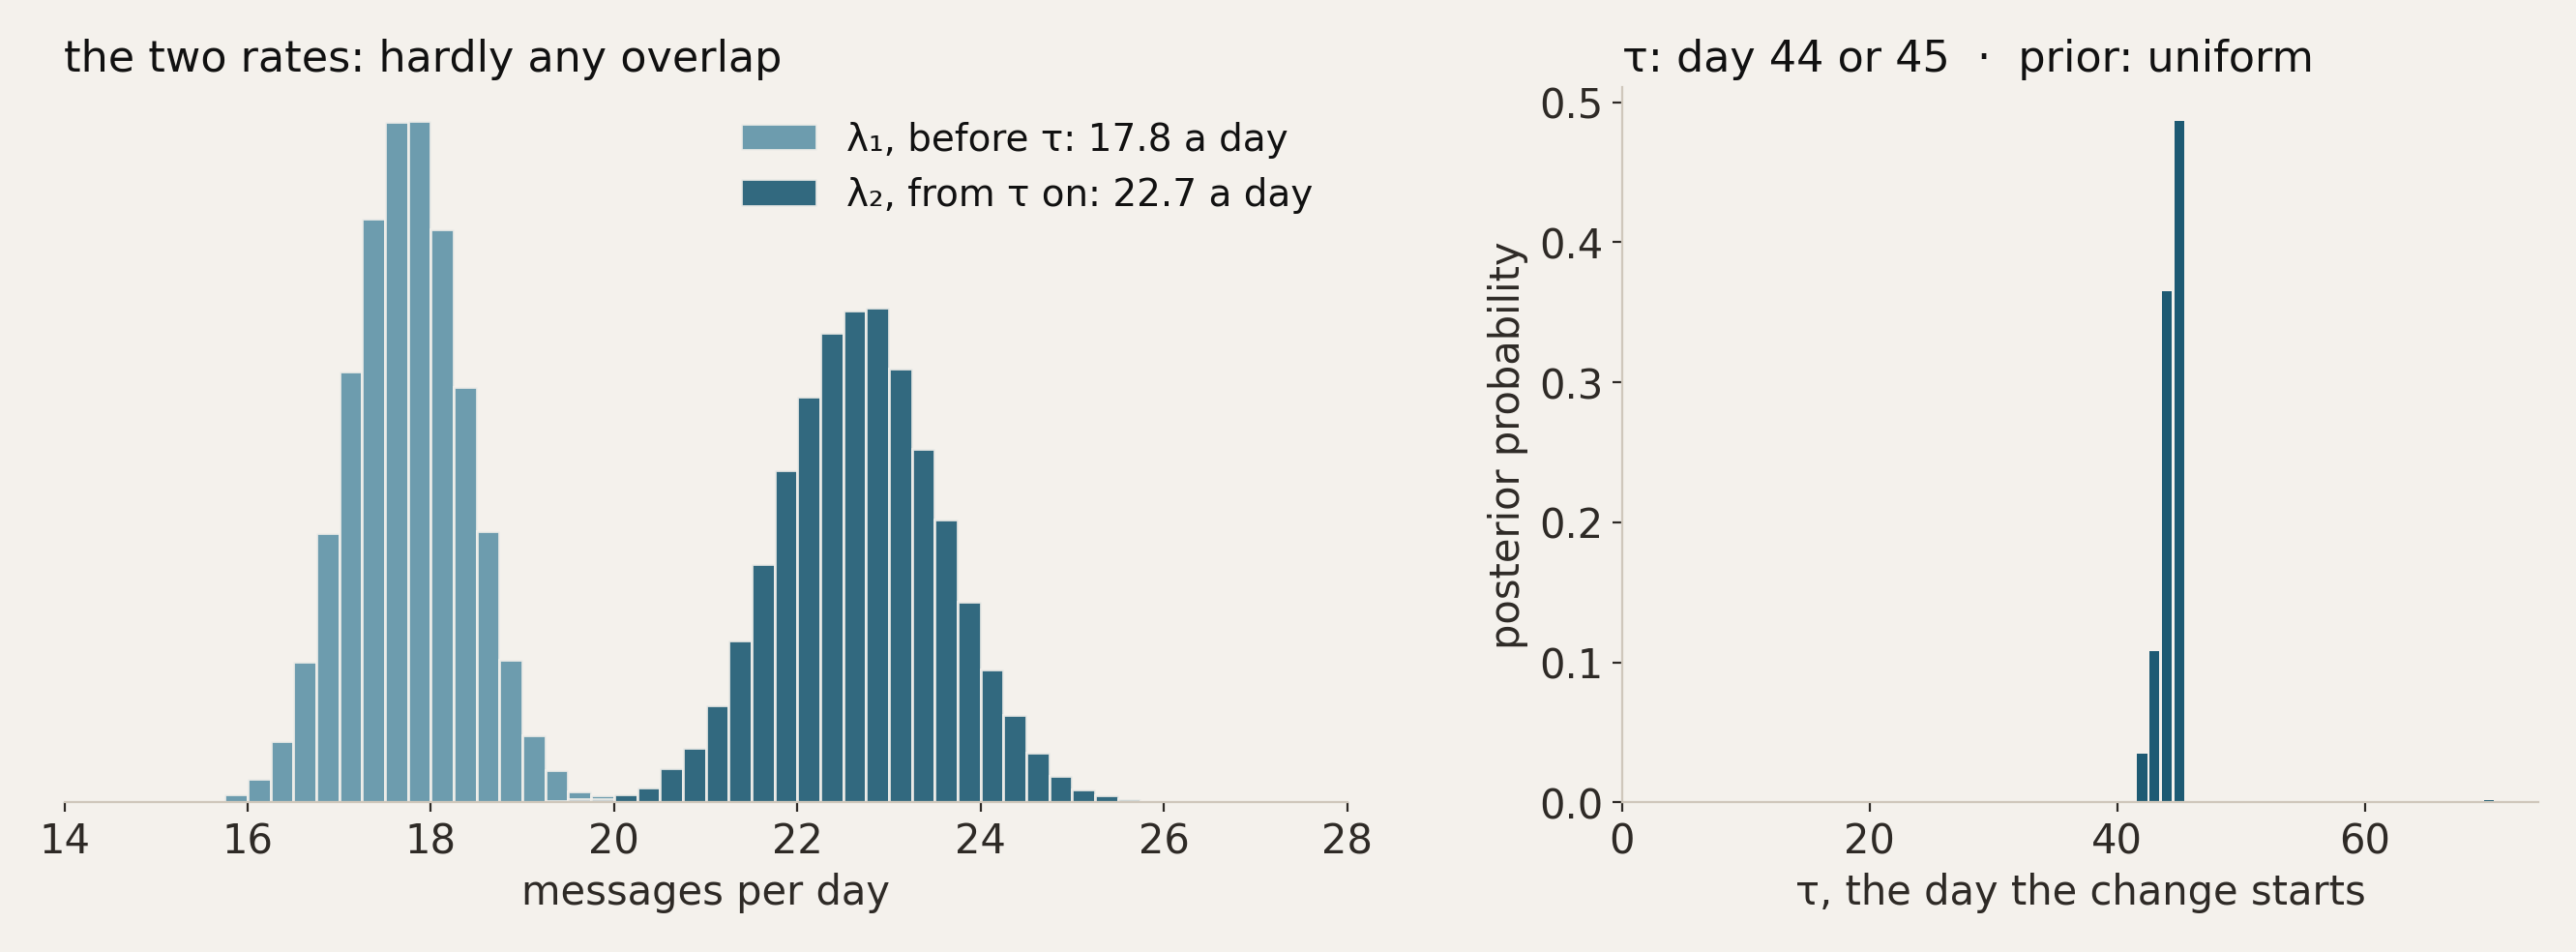
\includegraphics[width=\textwidth]{lesson4/texting_book.png}
\caption{The book's model. Left: the two rates. Right: the switch day $\tau$.}
\label{fig:texting-book}
\end{figure}

The shuffle said a difference this size turns up in one shuffle out of seven. Same data, very different confidence.

\subsubsection{Are those assumptions right?}
Where does the difference come from? When we discussed this in class, the right objection came from the room: look at the spread. The book's method is fine; the question is whether its assumptions hold. A Poisson assumes $\Var(X) = \E[X]$, so a day with an average of $18$ messages varies by about $4$ either way. These days run from $0$ to $72$: the variance is around $155$ to $250$, against a mean of $18$ to $23$. The assumption is violated, and because the Poisson underestimates the day-to-day noise, it is far too sure about each rate. That is why the two rates hardly overlap in the book.

Keep everything else in the book's model the same and only let the days vary more, with negative binomial counts instead of Poisson counts. Then no day stands out as the switch any more, and the probability that the second period is busier drops from $0.998$ to $0.59$. If you knew in advance that something happened on day $45$, it is $0.94$: a likely increase, not a certain one.

\begin{figure}[H]
\centering
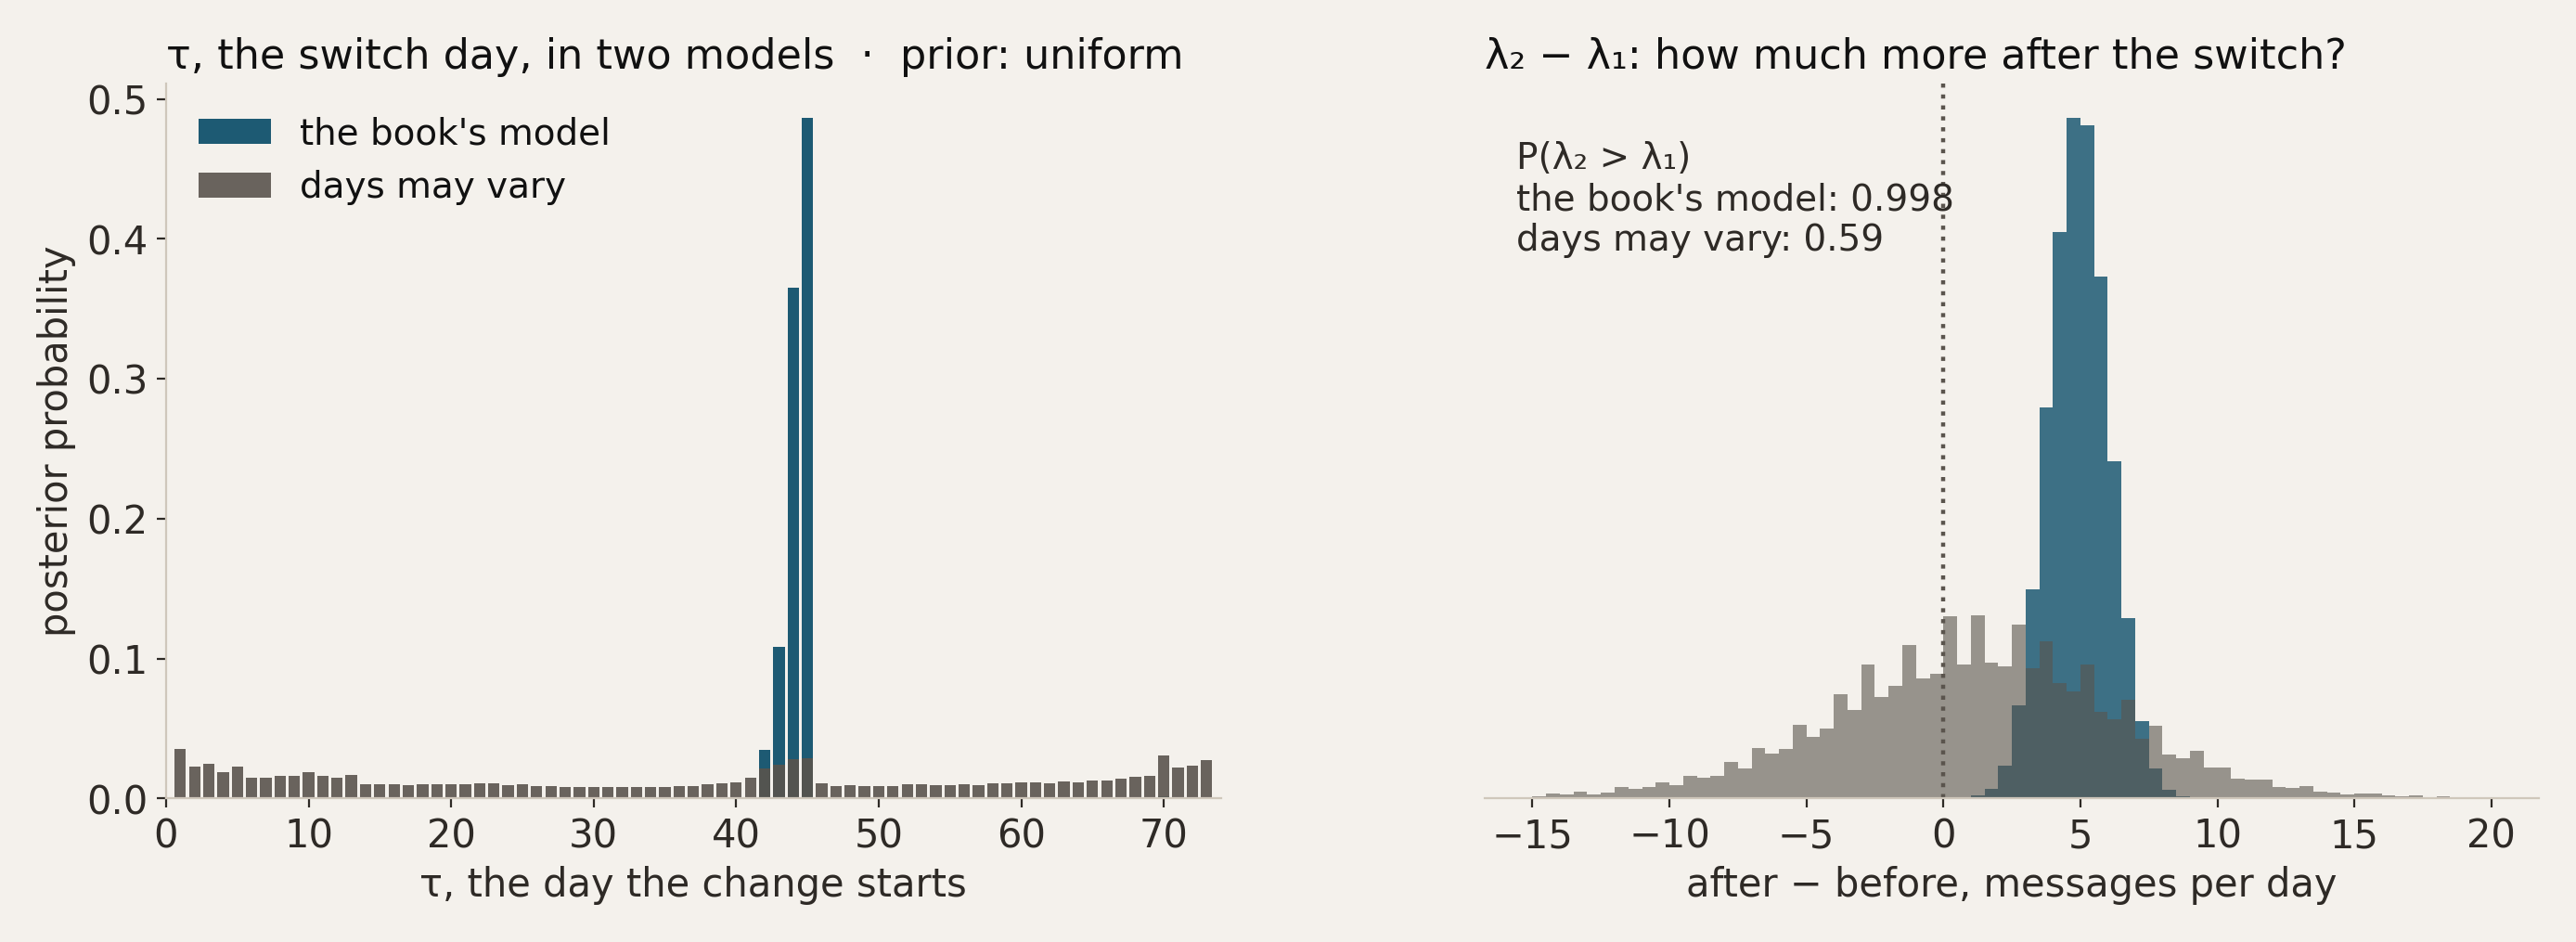
\includegraphics[width=\textwidth]{lesson4/texting_switch.png}
\caption{The same model with days that may vary.}
\label{fig:texting-switch}
\end{figure}

The technique is elegant; the distribution was wrong. The careful conclusion of the shuffle test turns out to be the more reliable one. There is a broader lesson here: you can model the same phenomenon in many ways, and depending on how you look, you get a different answer. A good reason to reject a model is a violated assumption, not a preference for a different answer.

\subsubsection{Searching for the day costs you the evidence}
There is one more thing hiding in the question ``did the texting change?'', and it is perhaps the most important point of this lesson. There are two different questions.

\begin{enumerate}
\item \emph{The day is known in advance.} Something happened on day $45$, and I want to know whether the texting went up after it. That is one comparison. The shuffle test gives $7\%$ (now counting only shuffles where ``after'' is busier), and the model with varying days gives $0.94$.
\item \emph{The day is searched in the data.} I don't know whether anything happened, so I try every split and keep the biggest difference. Now chance gets a try at every possible split; here $55$ of them, with at least ten days on each side. The best of those $55$ tries beats $+5$ in $45\%$ of the shuffles. The model gives $0.59$.
\end{enumerate}

\begin{figure}[H]
\centering
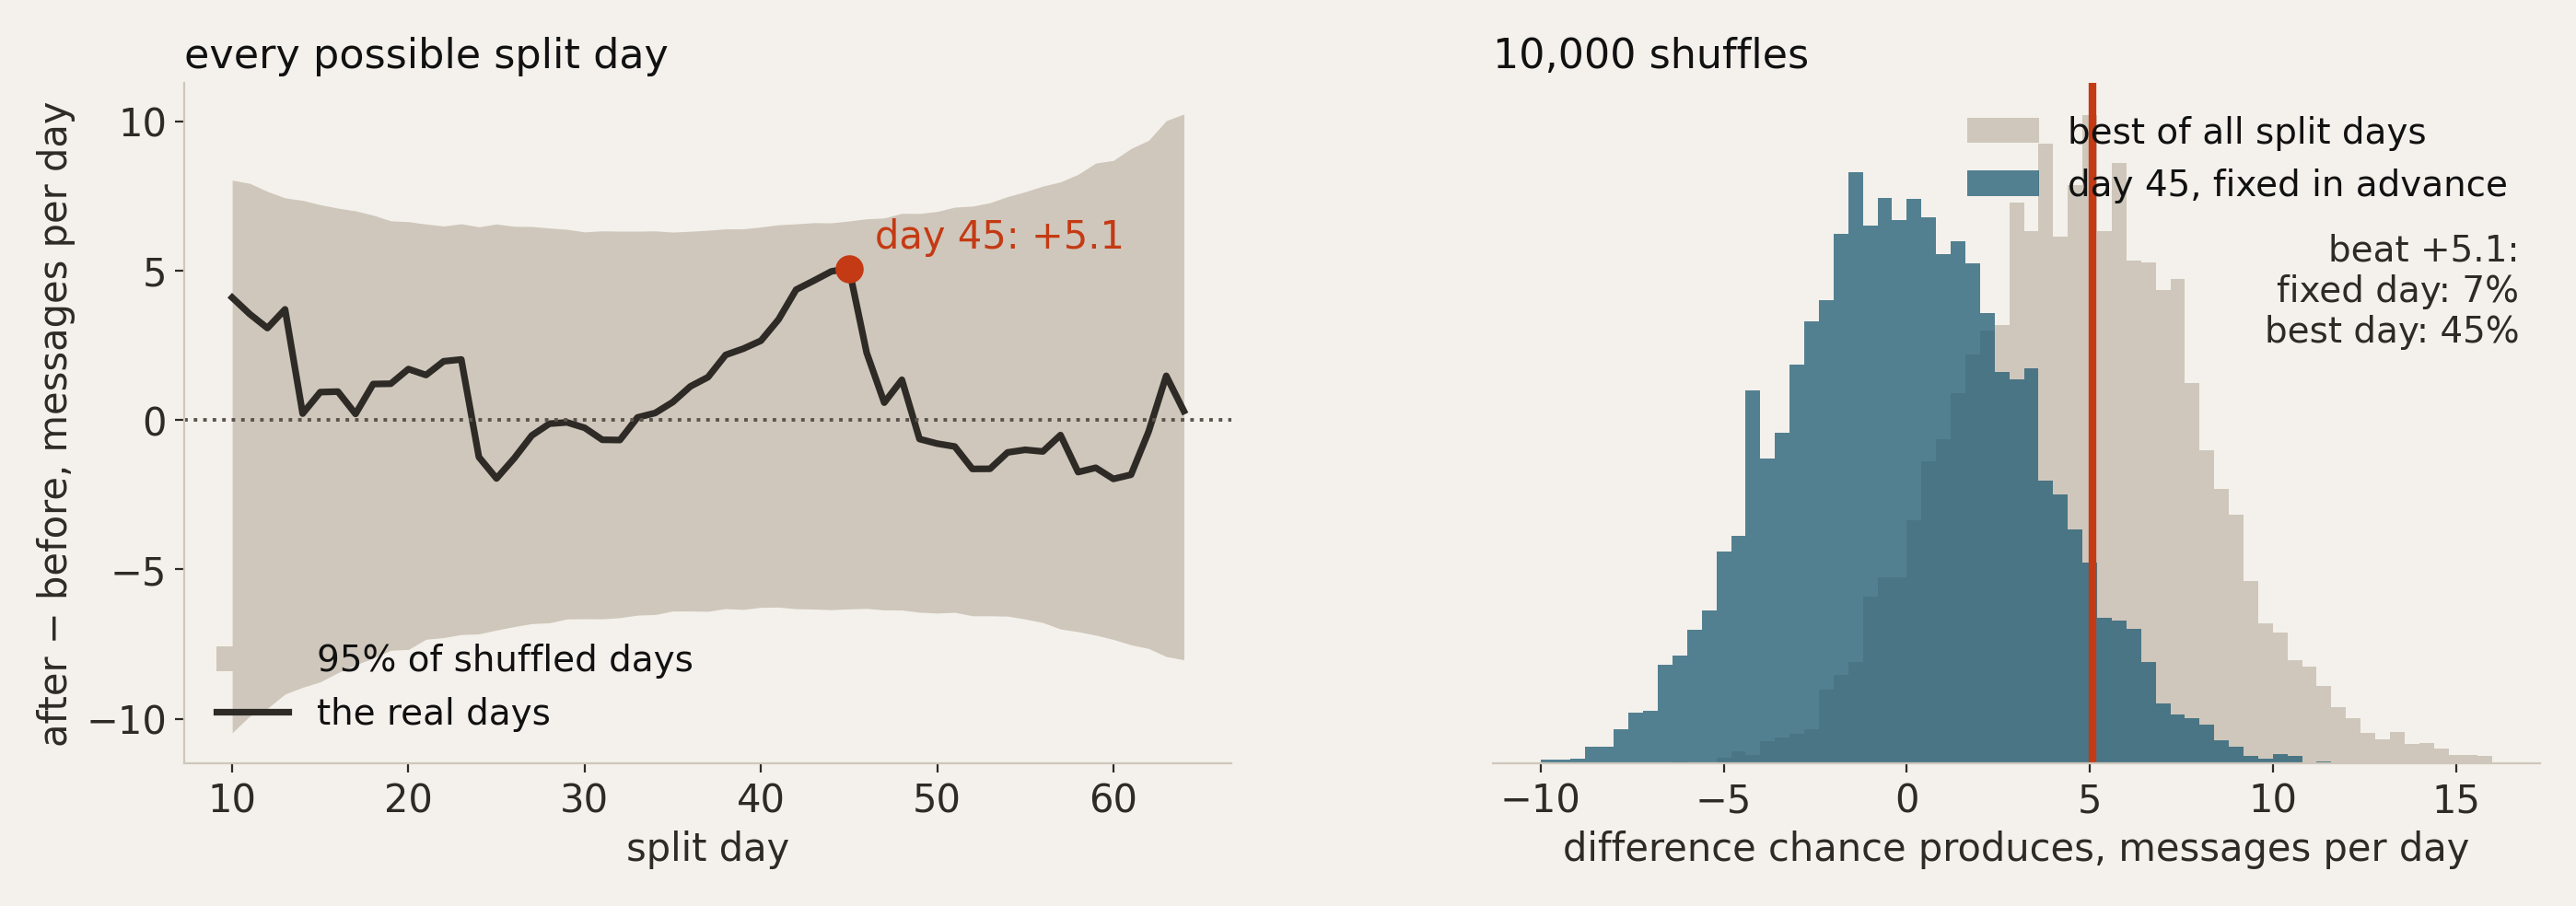
\includegraphics[width=\textwidth]{lesson4/texting_search.png}
\caption{Left: the difference for every possible split day; the grey band is what shuffled days do. Right: the biggest difference chance finds when it may pick the day (grey), against the difference at a day fixed in advance (blue).}
\label{fig:texting-search}
\end{figure}

A difference of $+5$ is unusual for one fixed day and ordinary for the best of $55$. Day $45$ looks special because it was picked for looking special. An event you know beforehand turns $55$ questions into one. The Bayesian model does the same bookkeeping automatically: with $\tau$ unknown, it has to spread its belief over all days, and with realistic day-to-day noise no day stands out. With Poisson counts the data look so decisive that this cost disappears, which is why the book could find the day and be sure of it at the same time.

I like to explain this with dice. Put $100{,}000$ people in a hall and let each of them roll a die six times. If you afterwards find someone who rolled six sixes, that is not proof of special powers, only of a big hall: with that many people you should expect it. But if you point at someone \emph{beforehand} and say ``this person has special powers'', and they roll six sixes, that is spectacular. And if they do it a second time, you call the army. Predicting the future afterwards is easy; the trick is doing it beforehand.

This has a practical consequence for your own analysis. If you know beforehand that a trip, a hospital stay or the weeks of morning sickness in a pregnancy define your labels, you can simply use those labels. A short period or a small number of observations is then not a reason to give up, because a shuffle test on labels that were fixed in advance can still come out very significant. Name the event before you look. Searching first and testing afterwards finds a switch in almost any series.

\subsubsection{Same lift, two verdicts}
The same test, on two Ubuntu chat channels: is a release day busier than an ordinary Thursday? The labels are shuffled 2,000 times, as in notebook 04.4. In both channels a release day is busier, by a factor of about one and a half. In the small Italian channel, \#ubuntu-it, release days are $41\%$ busier, but the real difference sits at the edge of the shuffle cloud: $p = 0.07$. Ten days of a rate that wanders this much can't settle it. In the big channel, \#ubuntu, release days are $47\%$ busier, and far outside anything the shuffles produce: $p < 0.001$.

\begin{figure}[H]
\centering
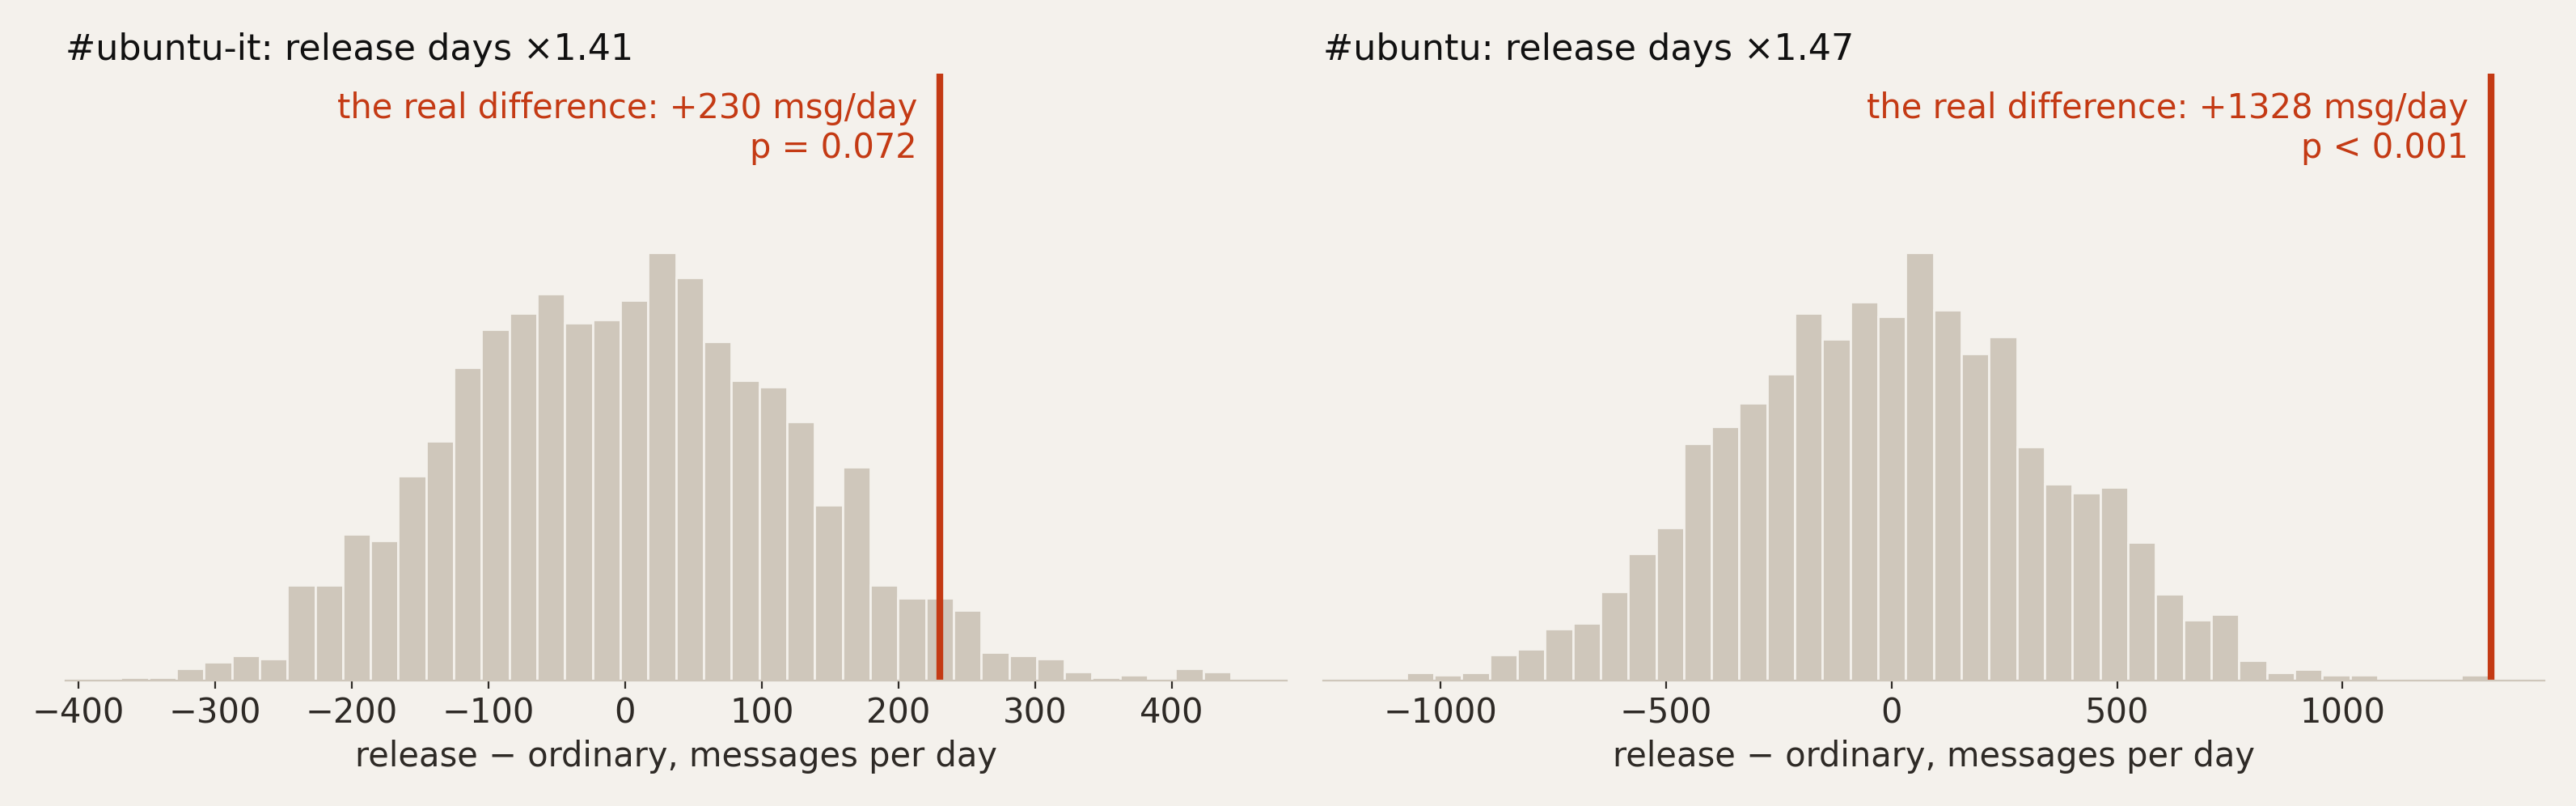
\includegraphics[width=\textwidth]{lesson4/irc_null.png}
\caption{Release days against ordinary Thursdays in two channels, 2,000 shuffles.}
\label{fig:irc-null}
\end{figure}

Same effect, different evidence. The reason is the spread of the ordinary days: in \#ubuntu-it they wander by two thirds of their mean, in \#ubuntu by a third, because many people averaging out make days more alike. There is no sharp line between chance and change: the further outside the cloud, the more convincing.

\againconcretely
A $40\%$ busier release day is borderline in a small channel and unmistakable in a big one. The noise decides. Compare before and after, then ask how big a difference chance alone makes; shuffling the labels answers that without assuming a family. The noisier the ordinary days, the more event days you need before you can see a change, and that spread is something you can see before any event happens.

% ─────────────────────────────────────────────
\subsection{Is my model done?}
\label{sec:residuals}
The last question. Fit a model, subtract it from the data, and look at what your model can't explain:
$$\text{observed} - \text{model} = \text{residual}.$$
The model doesn't need to be a statistical model; a simple formula or a straight line will do. What matters is what the residual looks like.

\begin{itemize}
\item \textbf{The residual looks like chance:} errors around zero, from a plausible family, with no pattern over time. Then you may be done. \emph{May}: a cause you never measured also looks like chance, and adding it could still make the spread much smaller. That is the epistemic uncertainty from the start of this lesson.
\item \textbf{The residual has a pattern:} a step, a drift, a bend. Then your model is missing a mechanism, and when the pattern starts is often the most interesting finding. That doesn't make the model useless; whether it is good enough depends on what you need.
\end{itemize}

Good enough is a goal, not a statistic. If you bet on something that is fifty-fifty, a mechanism that picks the right side $51\%$ of the time makes you rich, as long as you can bet often enough in a row and the mechanism stays consistent. You don't need $99\%$. (Living through the $49\%$ is the hard part, so write an algorithm for it.) What you do need is to communicate clearly what your model does and does not capture.

\subsubsection{Before vaccination, the residual looks like chance}
For this example I deliberately use data that is not chat data, because what transfers is the loop of modelling and checking, not the dataset. The data are the public Dutch COVID figures. A pipeline prepared them: daily deaths from the cumulative count, shifted fourteen days back next to the positive tests that led to them, and a seven-day average against the weekly reporting rhythm. The model is simple. On average, people who die of COVID die about two weeks after their infection, so deaths two weeks later are a fixed fraction of positive tests: a straight line. Fitted on the $85$ days from 13 October 2020 to 5 January 2021, before vaccination started, the line is
$$\text{deaths}_{t+14} \approx 0.0065 \times \text{positive tests}_t + 20.$$

\begin{figure}[H]
\centering
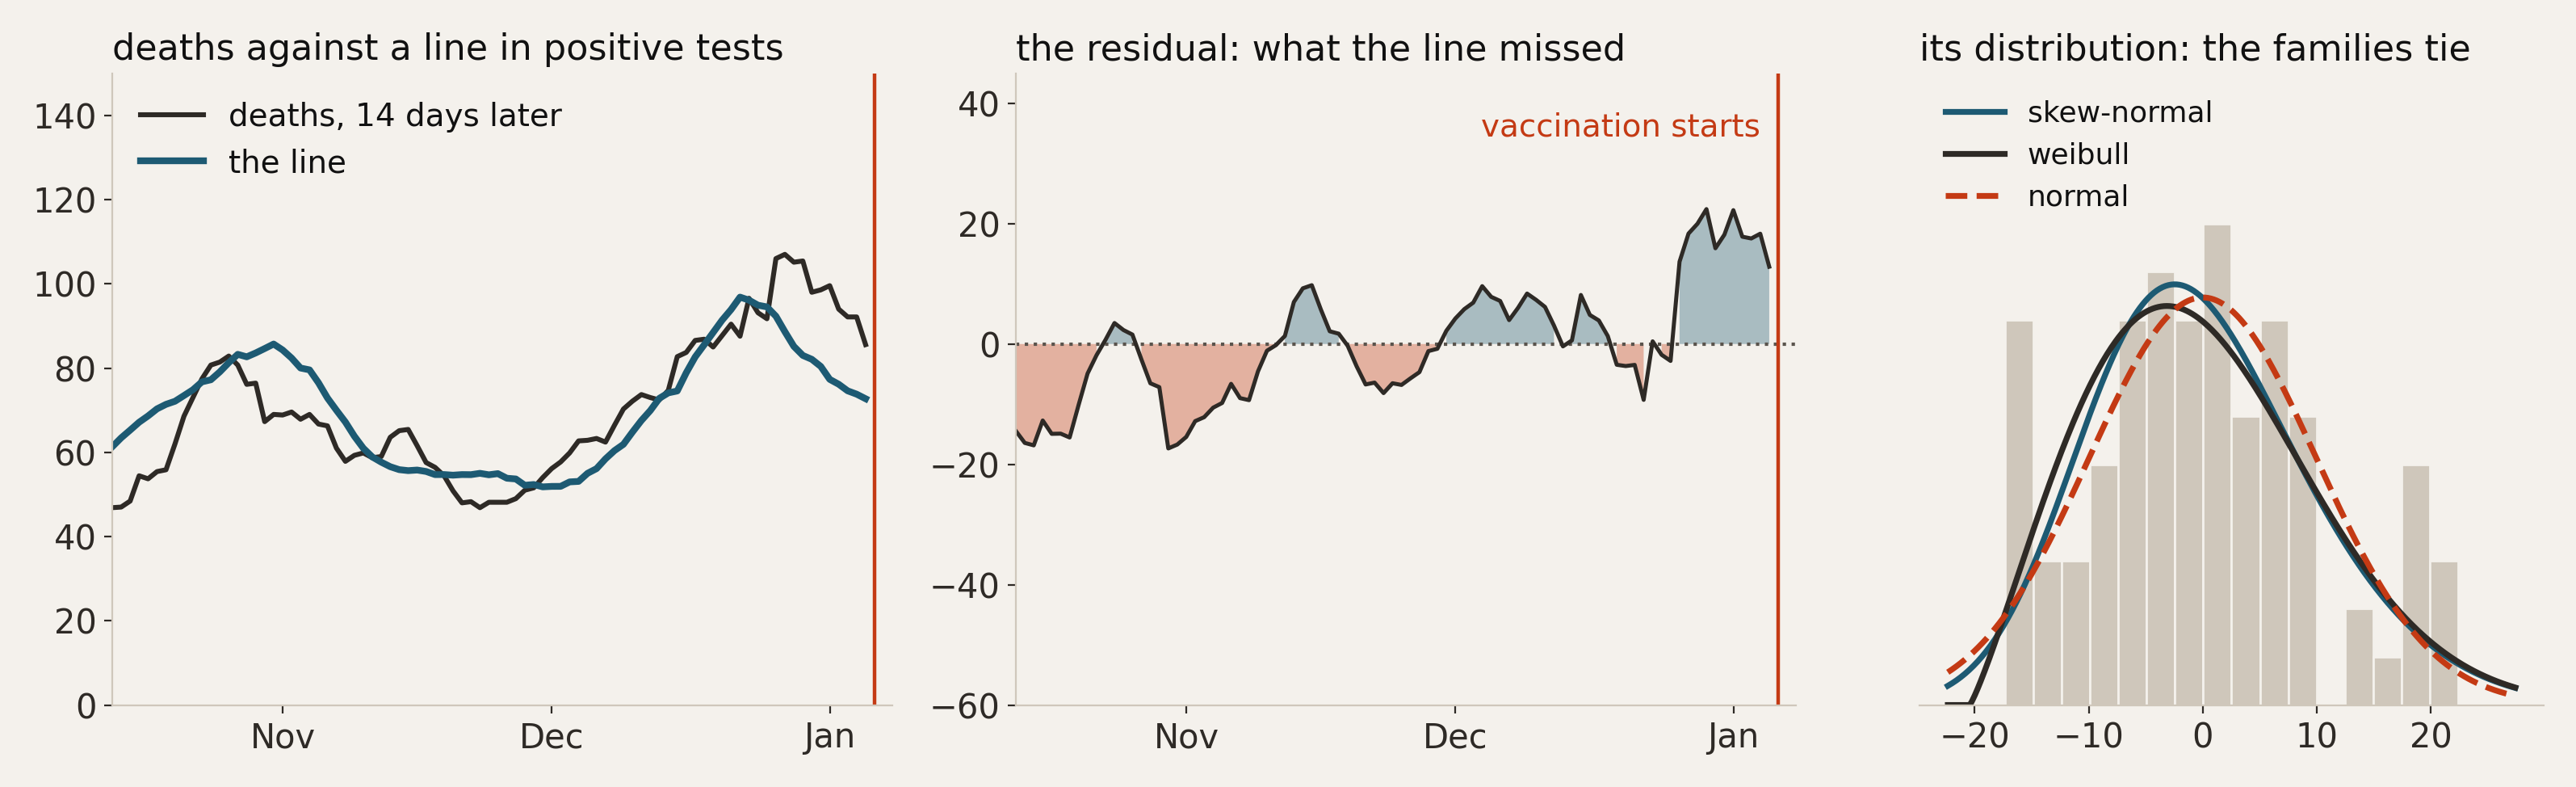
\includegraphics[width=\textwidth]{lesson4/covid_before.png}
\caption{Before vaccination (85 days). Left: the model. Middle: what the line missed. Right: its distribution.}
\label{fig:covid-before}
\end{figure}

On that window the residual waves around zero with no drift (figure~\ref{fig:covid-before}); the last week runs high at the winter peak. There is also a bump around Christmas, and in class the temptation was to read it as the start of an upward trend. Be careful which pattern you think you see: if that were a real trend, it would mean the virus became deadlier over time. Much more plausible is that the Christmas holiday and the lockdown rhythm run through the data. When we fit distributions to the residual, six families fit within a few points of each other and none is rejected. Errors the data can't tell apart: that is what chance looks like.

\subsubsection{The residual reveals what the model missed}
Now fit the same kind of line on all $232$ days, from October 2020 to June 2021 (figure~\ref{fig:covid-full}). Nothing in the model knows that a vaccine exists. From March it predicts more deaths than happen, month after month. The residual changes character: positive through the winter wave, and then from 27 February to the end a long negative run that never comes back. Every family is rejected; the best is the uniform, which is what a fitter says when the errors lie along a trend instead of around zero.

\begin{figure}[H]
\centering
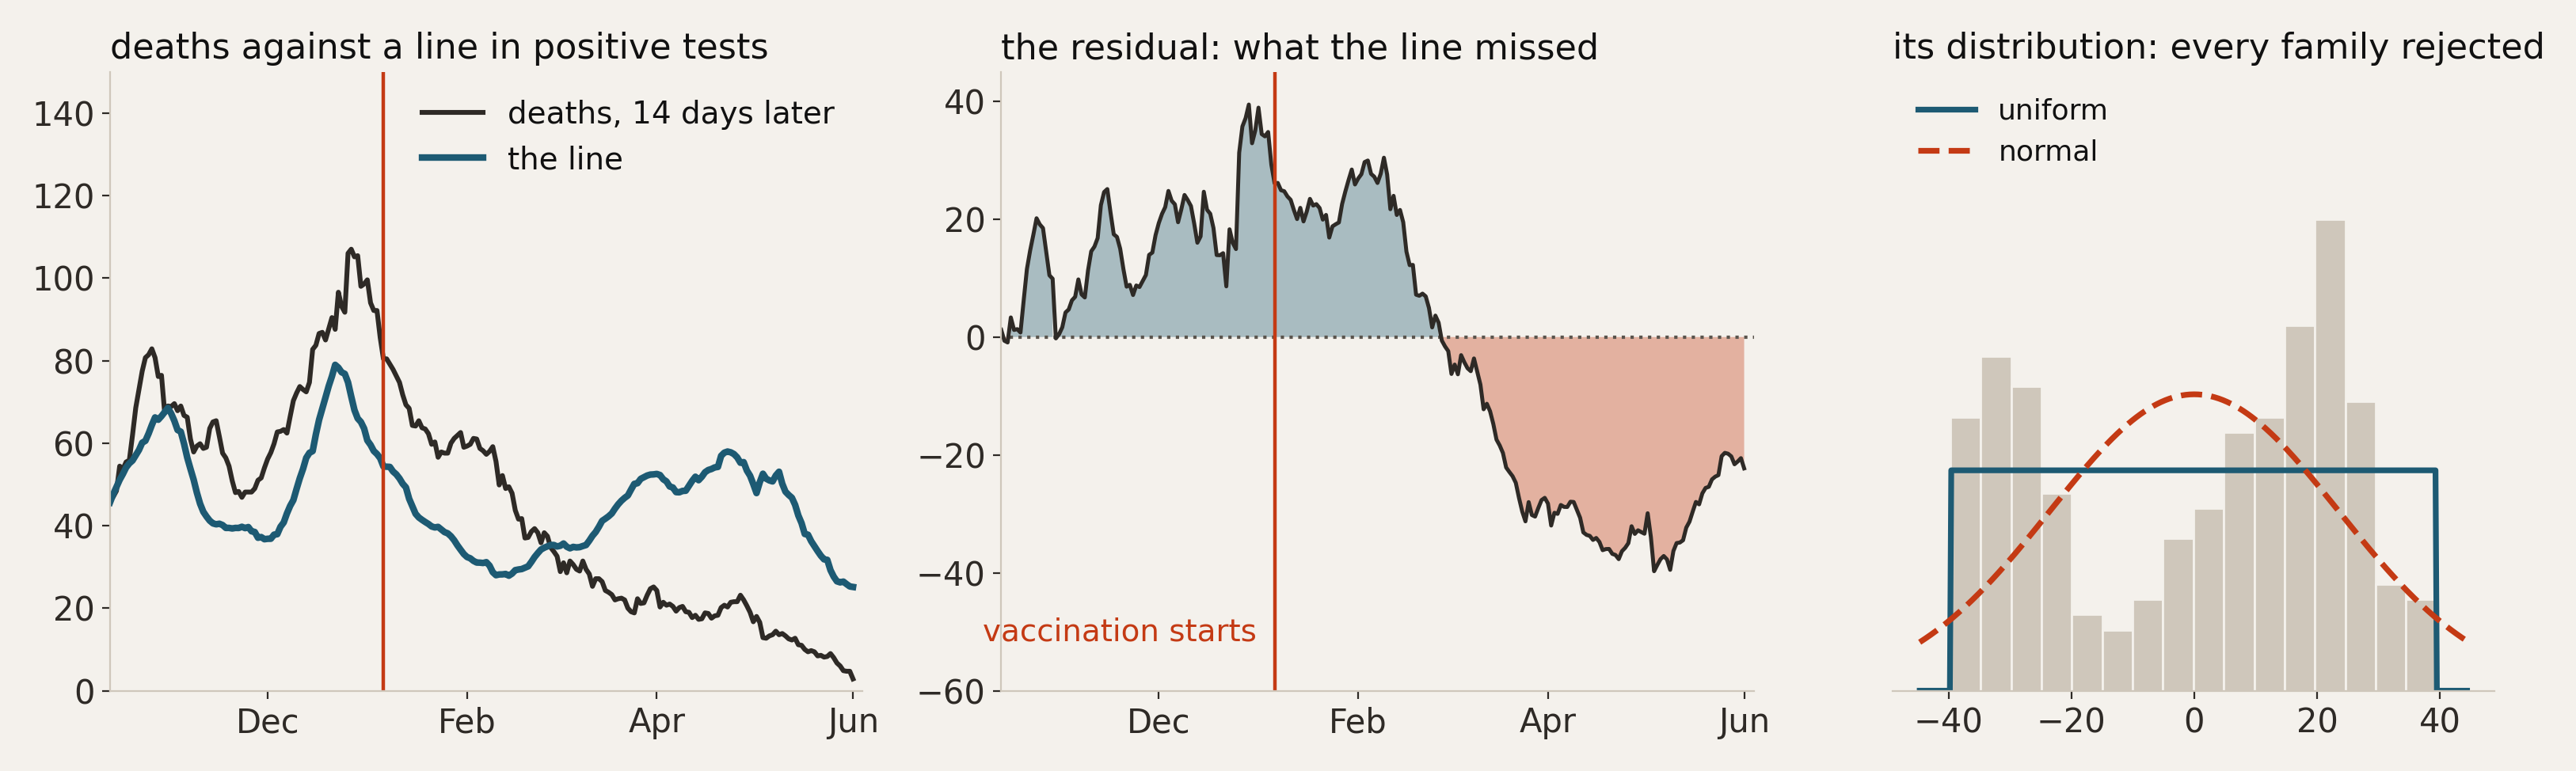
\includegraphics[width=\textwidth]{lesson4/covid_full.png}
\caption{The same kind of model over 232 days, October 2020 to June 2021.}
\label{fig:covid-full}
\end{figure}

The residual is pointing at a process the model left out, and at roughly when it started: after vaccination, the same number of positive tests comes with fewer deaths. The correlation between tests and deaths over the whole period looks weak, but it is really two different random processes. Notice what the residual does and does not do. It dates the change; it does not prove the cause. Better treatment, or a change in who got tested, could leave a similar run.

\againconcretely
One straight line, two windows. Before vaccination, the line was a fine model: what it missed looked like chance, and for many purposes the line is good enough. Over the full window, the residual has a run with a start date: a mechanism is missing, here vaccination, and that pattern is the most informative thing the model produced. Next lesson, notebook 05.3 hands you this residual and asks you to write the missing mechanism into the model.

% ─────────────────────────────────────────────
\subsection{The five questions, answered}
\label{sec:lesson4-summary}
\begin{table}[H]
\centering
\begin{tabularx}{\textwidth}{@{}l X@{}}
\toprule
\textbf{Question} & \textbf{Answer} \\
\midrule
What is a distribution? & A model of what you can predict about randomness: every possible outcome, with shares that sum to one. \\
Which distribution fits my data? & First reason about a model that fits the underlying process, then fit, then check. Never the other way around. \\
What is an outlier? & It shows what you modelled as ``expected''. \\
Did something change, or is it chance? & Only if the difference is bigger than chance alone makes. Name the event before you look. \\
Is my model done? & Study the residual, and wonder which patterns your model did not pick up. \\
\bottomrule
\end{tabularx}
\end{table}

Notebooks 04.1 to 04.5 work through each of the questions, ending on your own chat.

\subsection{Feedback on your distribution plots}
\label{sec:showing}
In the second half of the lesson we discussed the distribution plots you made of your own data. The same points came back again and again, so I collect them here.

\textbf{One message, in half a second.} A good visualisation works pre-attentively: the reader picks up the message within about $500$ milliseconds, before they start reading. That only works for simple messages: something is bigger, smaller, shifted, or happened. Two clearly different things, not more.

\textbf{Reduce the clutter.} Remove the grid. Bring the palette back to two meaningful colours, for example grey for ``before'' and one colour for ``during''. Six lines of legend where one label next to the line would do is noise. Labels like ``axis is logarithmic'' or ``line is a fitted lognormal'' can go if the axis already says so.

\textbf{One visualisation, not two.} People usually show two plots because they cannot choose. Two plots are only defensible if together they tell one story.

\textbf{The title must match what the data can carry.} A neutral title is a waste; you are allowed to bring a message. But the message has to be backed up by the data. ``Our first holiday together made our group of friends closer'', based on the observation that messages got longer, is too big a leap: long messages can also be long arguments about who still owes money for that dinner. Either choose a less ambitious title, or dig deeper into what those messages are about. Always ask yourself: do I have the data to back this up?

\textbf{Show a real distribution.} Follow the three rules of definition~\ref{def:distribution}, and decide whether you are showing probabilities (discrete) or a density (continuous). Put \emph{density} on the axis of a continuous plot. A y-axis that runs from $0$ to $75\%$ under a smooth fitted curve tells the reader you haven't made that choice.

\textbf{Report the shuffle test.} If you compare two distributions, the number your reader is waiting for is how likely the difference is under chance: ``$p$-value after $10{,}000$ shuffles''. Not the standard deviation of your lognormal fit. Parameters are only interesting when you compare two processes, such as the two rates before and after day $45$.

\textbf{Be careful with log scales in a presentation.} A log axis compresses, and makes two distributions look alike that are very different on a normal axis. Your audience cannot undo the logarithm in their head.

\textbf{Know who you make it for.} Transparent histograms behind fitted lines are fine for a trained reader and noise for a business audience. That is a choice, not a matter of right or wrong.

\textbf{A null result needs tension.} Sometimes you find that nothing changed. That is interesting only if there was a strong expectation that something would. If nobody expected an effect, finding none is not a story; dig deeper.
\newpage

\section{Lesson 5: Modelling relationships}
\label{sec:lesson5}
The previous lessons each added a way of looking at data: comparing categories, following something over time, smoothing out a trend, describing randomness with a distribution. This lesson puts them together. A model of a relationship is a small formula with two sides: the number of people who die equals the number of people who test positive, times some factor. If you made your plots well, you should be able to write what they show as a formula like that. And every earlier lesson can be a building block in it: a category, a time effect, a smoothing step, a distribution for the part you cannot explain.

The lesson is organised around six questions:

\begin{enumerate}
\item \textbf{What} is a model? A simplification you choose. Never the whole truth, and never neutral.
\item \textbf{Why} keep a model simple? A computer can fit anything. People can only understand simple shapes.
\item \textbf{How} do you build a model? Look at the data, think about the world, add one thing.
\item \textbf{When} should you believe a pattern? If you look at enough things, you always find something.
\item What can a \textbf{correlation} hide? A variable you left out can reverse a correlation, or create one.
\item Can you \textbf{recognise} someone by how they type? A model that works can still be right for the wrong reason.
\end{enumerate}

The first two are about models in general, and about two ideas that almost every student brings in without saying them: that a model is true, and that a complex model is better than a simple one. The third is the heart of the lesson: the COVID model from the end of lesson 4, built step by step. The last three are about believing what you find.

% ─────────────────────────────────────────────
\subsection{What is a model?}
\label{sec:what-is-a-model}
A model is like a map: useful because it leaves things out. If you want to navigate, you don't use an aerial photograph. It has all the detail, and that is exactly what makes it hard to use. A map with a few colours and lines is better, because someone decided what to leave out\footnote{``The map is not the territory'' is Alfred Korzybski's phrase.}. A map of Utrecht that showed every stone would be as big as Utrecht. Modelling is the art of leaving things out, and that has three consequences.

\begin{itemize}
\item \textbf{A model is not true.} It is always an approximation, and there is always some distance between the model and the world. What you want is that the distance doesn't matter for what you use it for. Newton's laws describe how thrown objects move, and they work perfectly for everything you will ever throw. Near something very heavy, or at speeds close to the speed of light, they break down. Usually nobody cares, but your phone's navigation does: it times signals from satellites, and if it ignored the bending of time and space that Einstein described, you would not arrive where you wanted to go. So there you need the better model. Is Einstein's model then true? No; it is a better approximation, and it too breaks down in special cases. That is fine. It is still useful.
\item \textbf{A model is not objective.} This is the misuse of models that bothers me most: ``the data says so''. The data says nothing. You chose the shape, the variables and the slice of data, and someone else could choose differently with the same data. Leaving out the choices you made is lying by omission: nothing you said was false, but the other person no longer has a good map of what you did.
\item \textbf{A model is useful.} A good simplification shows you something you could not see in the raw numbers. You may treat discrete data as continuous and fit a normal distribution, knowing that it is not strictly right, as long as you can defend why. A Poisson distribution is not ``true'' either. It is also an approximation.
\end{itemize}

\subsubsection{Leonardo's earth: not true, still useful}
In his notebook on water and the earth, written in the early 1500s, Leonardo da Vinci drew the earth as a circle and a triangle: the circles are the oceans, the triangle the mountains and land masses\footnote{Leonardo da Vinci, \textit{Codex Leicester}, folio 35v, a detail.}. He knew very well that water and mountains look different. He drew it because a geometric shape lets you reason about something too big and too complicated to see whole.

\begin{figure}[H]
\centering
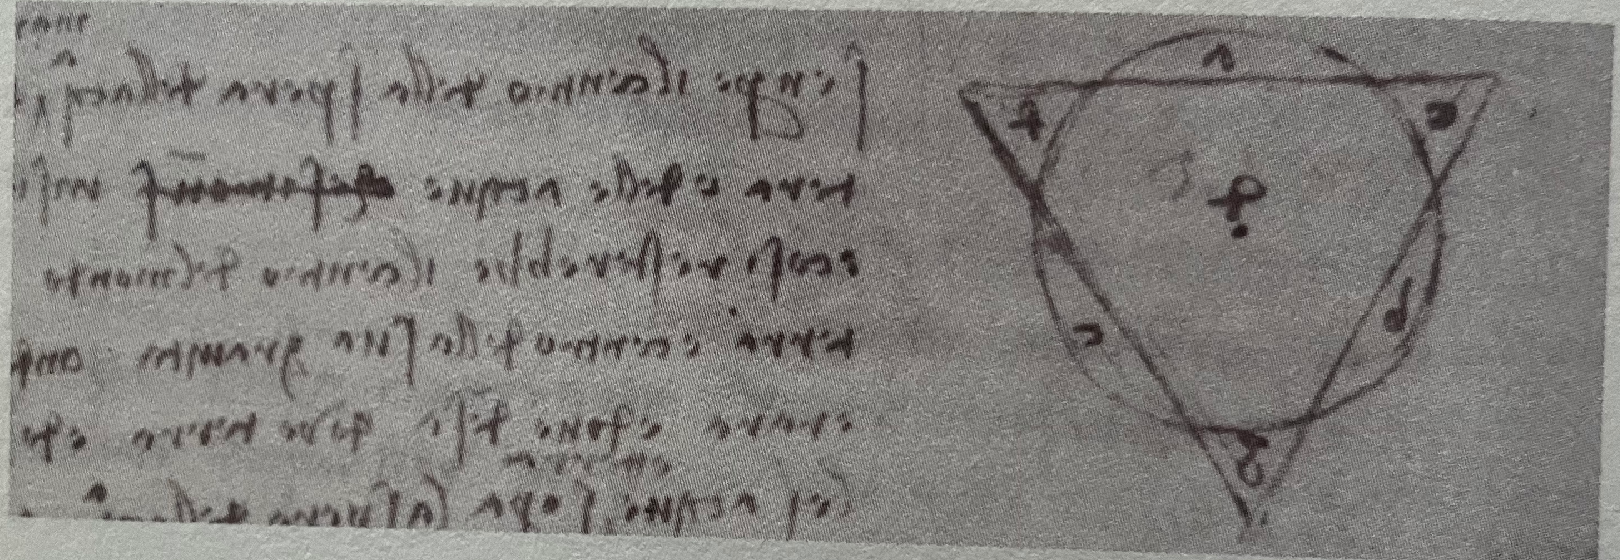
\includegraphics[width=0.8\textwidth]{lesson5/leonardo.png}
\caption{Leonardo's geometric model of the earth, from the Codex Leicester.}
\label{fig:leonardo}
\end{figure}

I find it a wonderful picture, even with everything we know now. It makes me see the earth as a drop of water floating through space, with the mountains as stones drifting in it. What is that useful for? I'm not sure; perhaps for thinking about the place of the earth in the universe. But it shows something new, even though its maker knew it wasn't true. Sometimes it is more interesting to ask \emph{what does the model show me} than to strive for the absolute truth.

\subsubsection{Three lines through the same cars}
The same point with data. Figure~\ref{fig:mpg} shows $398$ cars, their weight against their fuel economy in miles per gallon\footnote{The Auto MPG dataset from the UCI Machine Learning Repository.}. Heavier cars use more fuel; the question is what kind of relationship this is, and each of the three lines is a different claim about that.

\begin{figure}[H]
\centering
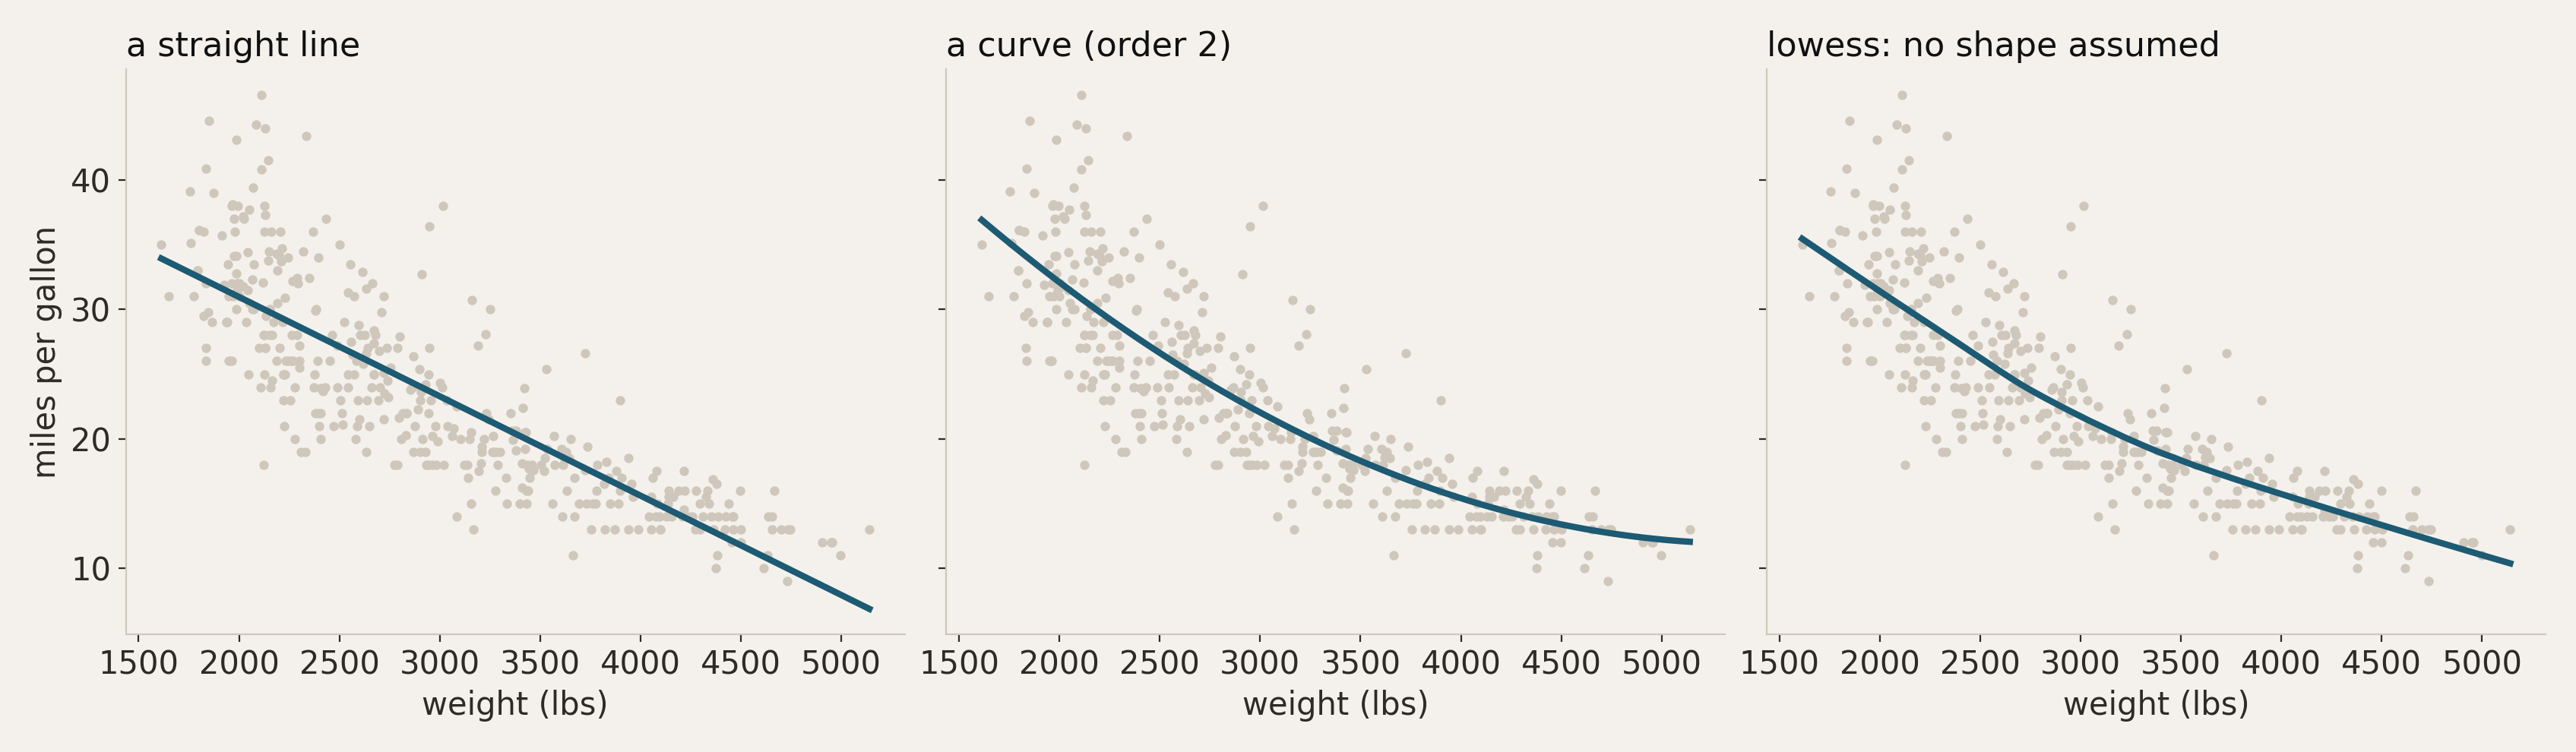
\includegraphics[width=\textwidth]{lesson5/mpg_claims.png}
\caption{398 cars, weight against fuel economy. A straight line, a line with a square in it, and lowess.}
\label{fig:mpg}
\end{figure}

The straight line says every extra pound costs the same. It is not a bad model: $R^2 = 0.69$, and the p-value is around $10^{-103}$. Both numbers are true, and neither tells you that the line has the wrong shape. The picture tells you immediately: the line sits below the lightest and the heaviest cars and above the ones in the middle. It is averaging a curve. Give the model one extra parameter, a term with a square in it, and it can follow the bend. Python then works out how much bend the data needs. On the right, \emph{lowess} draws what the data shows without any formula: a kind of moving average that turns the points into a line. It finds the same bend without being told there is one, but it is not really a model: it has no parameters you can read, and it doesn't predict. Use lowess to look; once you know the shape, choose a formula.

Which of the three is the true one? None. They are three claims, and you pick the one you can defend. If you are choosing a car, ``heavier cars use more fuel'' is all the model you need in your head; nobody needs a quadratic to buy a car. Different goals, different models.

\againconcretely
The map is not the territory. A model is a simplification you choose: the shape, the variables, the slice of data. So it is not true and not objective, and its value often lies precisely in what it leaves out. Students often hand in a model as if the data produced it. It did not: you made the choices. That is not a weakness; it is the job. The weakness is not knowing that you chose. And if you choose anyway, why choose something simple? That is the next question.

% ─────────────────────────────────────────────
\subsection{Why keep a model simple?}
\label{sec:why-simple}
The usual reflex is: why bother with simple models, when deep learning can learn anything from data? It is true that a computer with enough data can find very complex patterns, and for prediction that is often what you want. But people can only understand simple ones; there is a bandwidth to what we can follow. A deep learning model can have millions of parameters. It may predict well, but we can only understand what comes out of it, not what happens inside.

That matters more than it sounds. In my work for the province of Utrecht, imagine a brilliant system, even a flawless one, that says: build a roundabout there. Why? Trust me. That is not accepted, and it shouldn't be. People want to know why. A specialist who cannot explain everything can still give a metaphor or a story that makes it click, and then people are willing to stand behind the decision. People take responsibility for something only when they can understand, follow or trust it, and a model cannot take responsibility. If the roundabout turns out to be a mistake and you ask who is responsible, the answer cannot be ``nobody''.

Simple models are useful for three reasons. They give \emph{insight}: four simple shapes cover a surprising amount of the world, and each of them tells a story. They are \emph{restricted}: a model that can fit everything tells you nothing, while a simple model can fail, so when it fits, that means something. And precisely because a simple model is limited, it is most interesting where it fails. Every time a simple model goes wrong, you learn something: you think about what is happening there, model it, and look at what is left. That leftover, the residual, is only visible because the model is not flexible enough to swallow it.

\subsubsection{Four shapes worth knowing by name}
The four horsemen of modelling are the line, the sine, the exponential and the logistic. You don't need to know their formulas by heart; you need to recognise them by sight and know when to use them, because each of them is a sentence.

\begin{figure}[H]
\centering
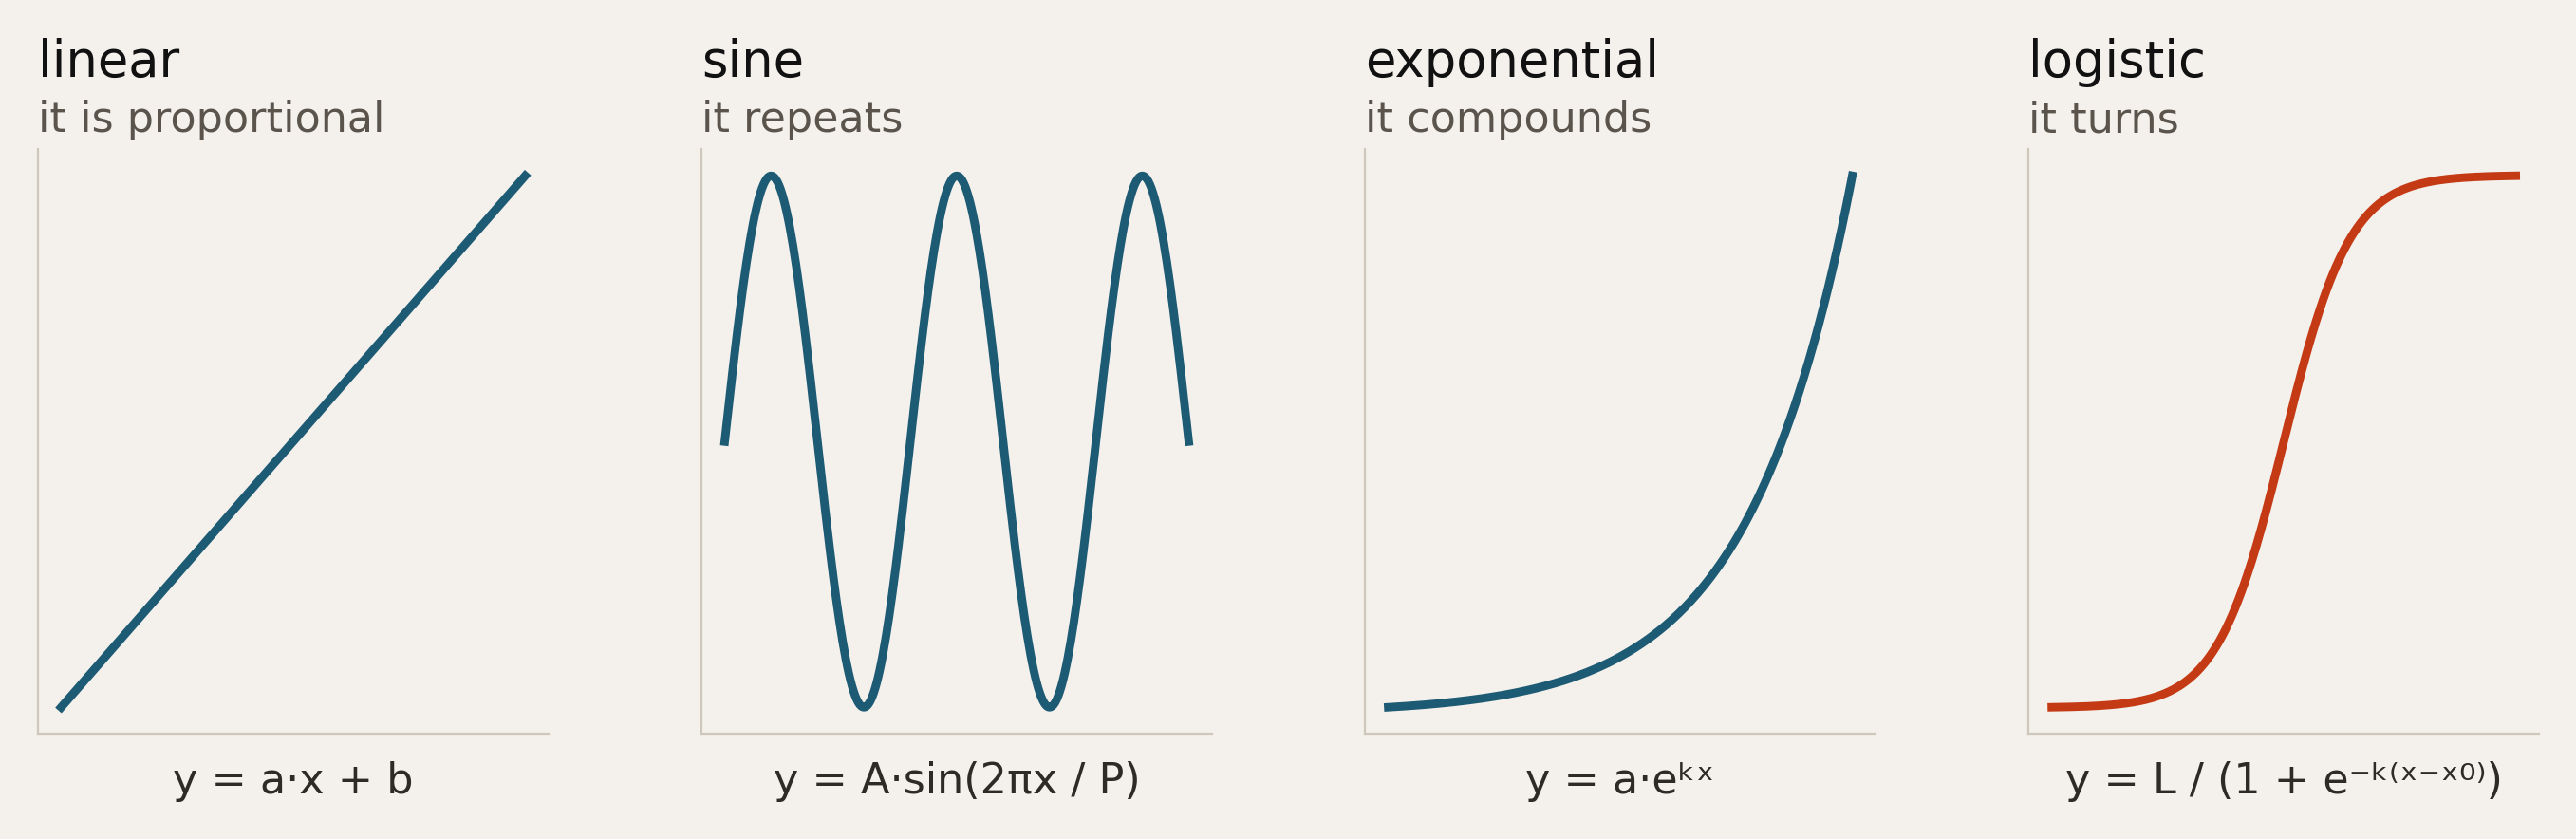
\includegraphics[width=\textwidth]{lesson5/horsemen.png}
\caption{The four shapes: linear, sine, exponential and logistic.}
\label{fig:horsemen}
\end{figure}

\begin{itemize}
\item \textbf{Linear} says \emph{proportional}: twice as much in, twice as much out. Price per kilo, or deaths per positive test: if a thousand people test positive and the factor is $0.01$, ten of them die.
\item \textbf{Sine} says \emph{it repeats}: the same pattern on a fixed rhythm, every day, week or season. Usually a sine is about time.
\item \textbf{Exponential} says \emph{it compounds}: every step multiplies by the same factor, so it grows faster and faster. Interest, or the start of an epidemic.
\item \textbf{Logistic} says \emph{it turns}: it grows like an exponential at first, then slows down and levels off at a ceiling. Turned around, it is a switch from one level to another.
\end{itemize}

My estimate is that these four, and sums and products of them, cover about $80\%$ of what you meet in data when you model it simply. The COVID model under question three uses three of them.

\subsubsection{Nothing in nature grows exponentially for long}
The old riddle: duckweed on a pond doubles every day and covers the whole pond on day $30$. On which day was it half covered? Day $29$, because the last doubling covers the second half. That is why exponential growth surprises people: for a long time almost nothing seems to happen, and then everything happens at once.

\begin{figure}[H]
\centering
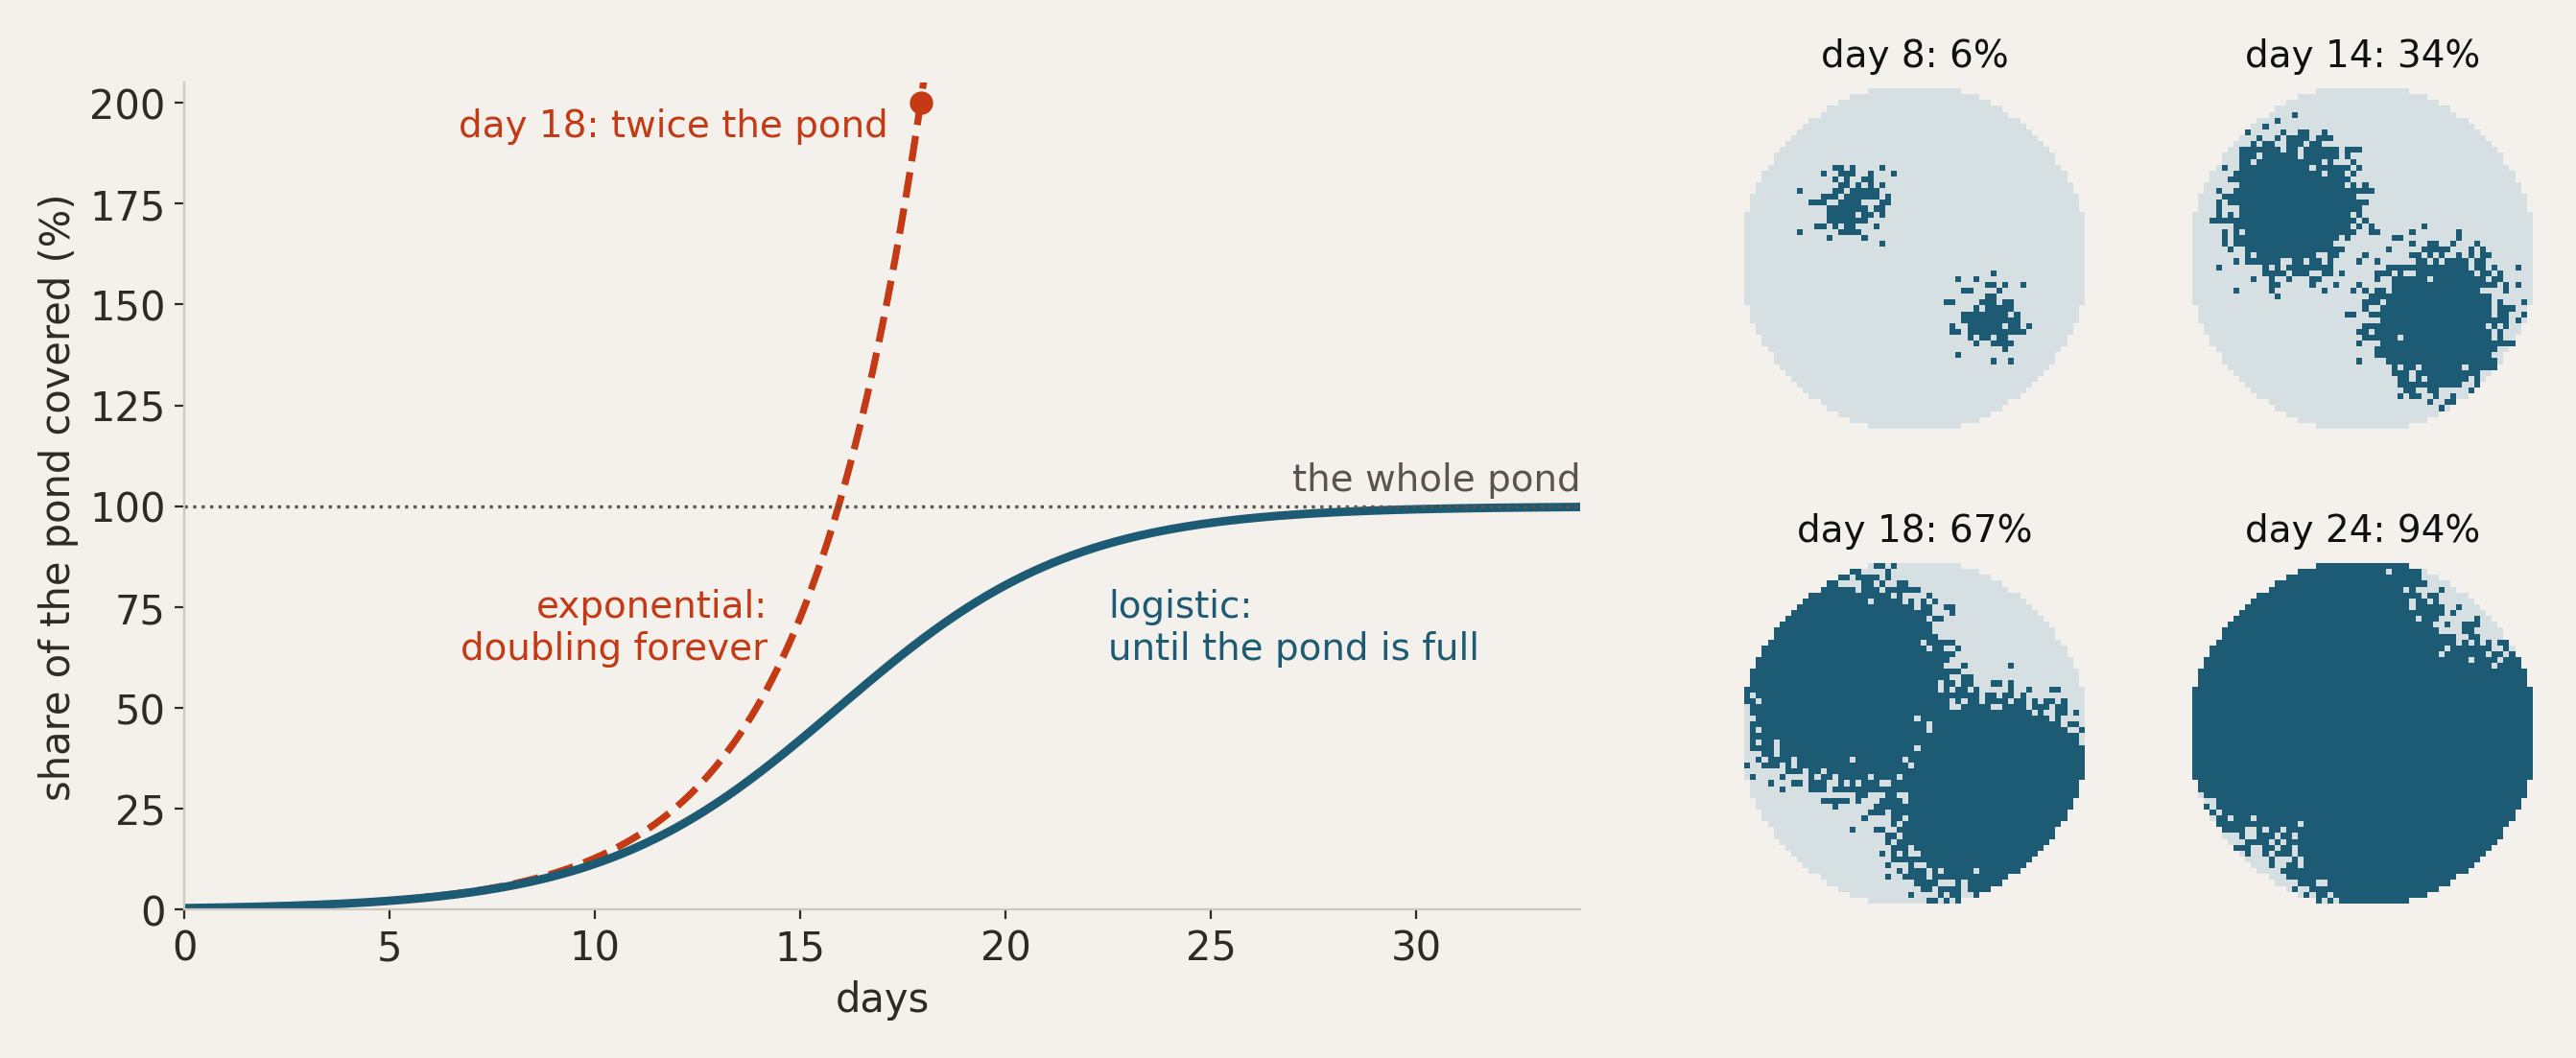
\includegraphics[width=\textwidth]{lesson5/pond.png}
\caption{Duckweed that doubles every two days, as an exponential and as a logistic. An illustration, not measured data.}
\label{fig:pond}
\end{figure}

A real pond adds what the riddle leaves out: the pond is only so big. In figure~\ref{fig:pond} the duckweed starts on $0.4\%$ of the pond and doubles every two days while there is room. The exponential keeps doubling and covers twice the pond on day $18$, which cannot happen. The logistic has the same start and the same doubling, and slows down as the free water runs out: half covered on day $16$, nearly full by day $25$. Natural systems never grow exponentially for long, because something always runs out: room, food, light, or for an epidemic, the people it can still infect. Markets don't keep growing either, however much shareholders want them to. The dangerous part is that in the first stretch of the curve you cannot see the difference between the two. If you extrapolate an exponential, think about where the edge of the pond is.

\subsubsection{A line plus a sine: four numbers, 93\% explained}
Monthly airline passengers from 1949 to 1960 combine two of the shapes: a line for the trend, and a sine for the summer holidays. A straight line in time, about $2{,}650$ more passengers every month, explains $85\%$ of the variation. Add a sine that repeats every twelve months, which costs two extra numbers (its amplitude and its phase), and that rises to $93\%$.

\begin{figure}[H]
\centering
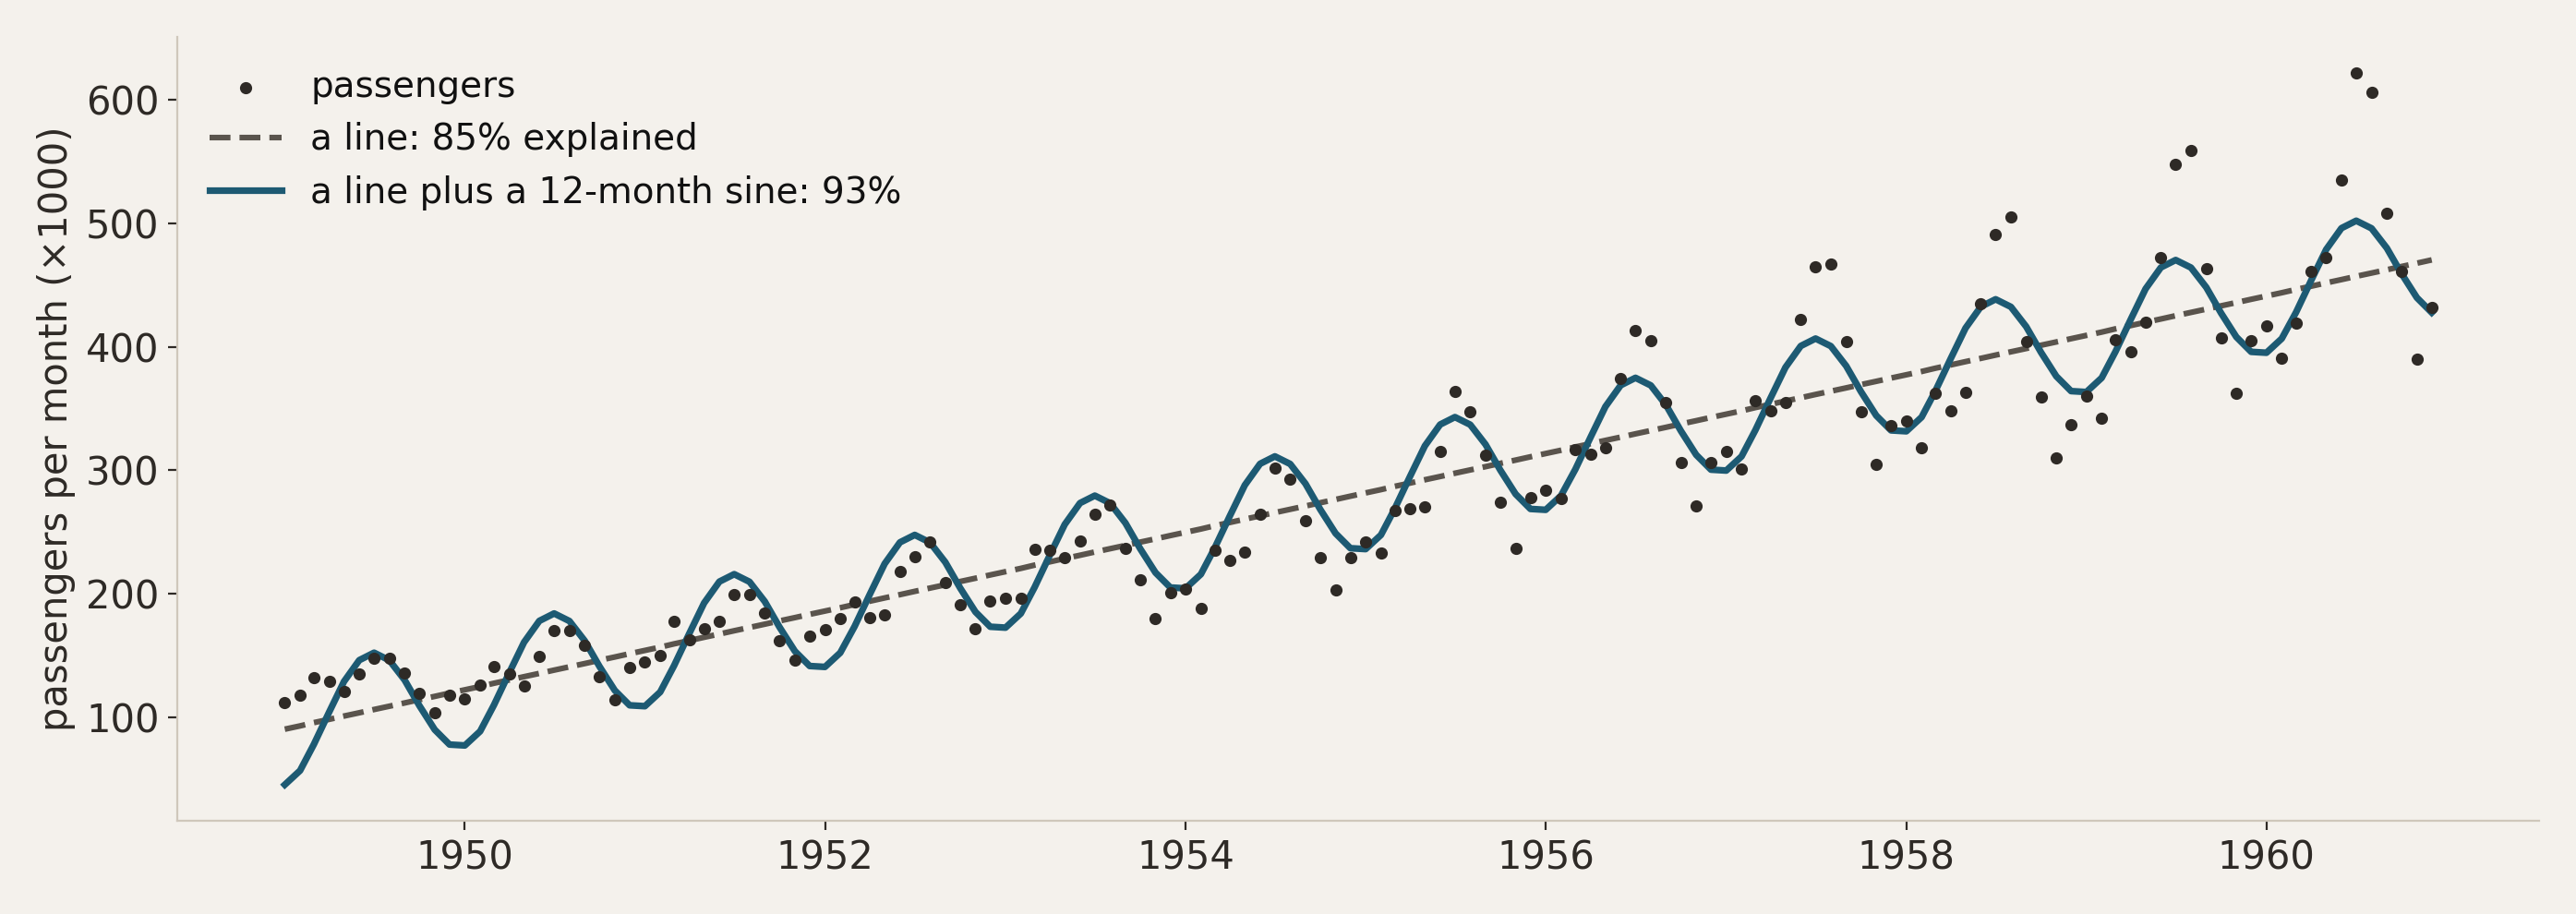
\includegraphics[width=\textwidth]{lesson5/airline.png}
\caption{Airline passengers, 1949--1960: a line, and a line plus a sine.}
\label{fig:airline}
\end{figure}

Four numbers in total, and you can say each of them out loud: how much the trend grows per month, how big the summer peak is, and when in the year it falls. That is a summary of a phenomenon in a few parameters you can interpret. And what is left over is honest and readable: the real summer swing gets wider as the trend grows, while a sine added on top of a line keeps the same width. You can only see that because the model is simple enough to read. How would you let the swing grow? Ask yourself which number in the formula of the sine sets its height, and what that height should depend on. This is an exercise in notebook 05.4 (section 5.4.3, ``a wave that grows''), so I leave it to you.

\subsubsection{A better fit is good, until you fit the noise}
Of course you want a model that fits better; that is what fitting is for. The problem is going too far. Every dataset is one sample, with its own accidents in it, and a model flexible enough to follow every point follows the accidents too: it models the noise. Lesson 4 gave the alternative. Noise is a factor in its own right, and you can model it: give it its own term, $\varepsilon$, say which distribution you expect, and check the residual against it.
$$y = f(x) + \varepsilon$$
The model then doesn't need to go through every point. As long as the data stays within the bandwidth of $\varepsilon$, it is a good description that respects the uncertainty.

The second point is about the goal. Sometimes the goal is prediction, and then a complex model is fine: nobody needs to read the weights of a neural network. But often the goal is people: a plot, a formula, a number with a sentence that someone else has to understand, check and act on. That artefact may well have been produced with the help of a complex model, but it still has to be understandable, because what people don't understand, they cannot work with. Fit the pattern, give the noise its own term, and hand over something people can understand.

\subsubsection{A model that can fit anything tells you nothing}
Twelve cars from the same dataset, spread over the weights (figure~\ref{fig:flexible}, top). A straight line fits reasonably: $R^2 = 0.72$. A polynomial of degree $11$ has twelve parameters for twelve points, so it goes through every single one: $R^2 = 1.00$, a perfect score. This is the result that tempts students: look, machine learning, a perfect fit.

\begin{figure}[H]
\centering
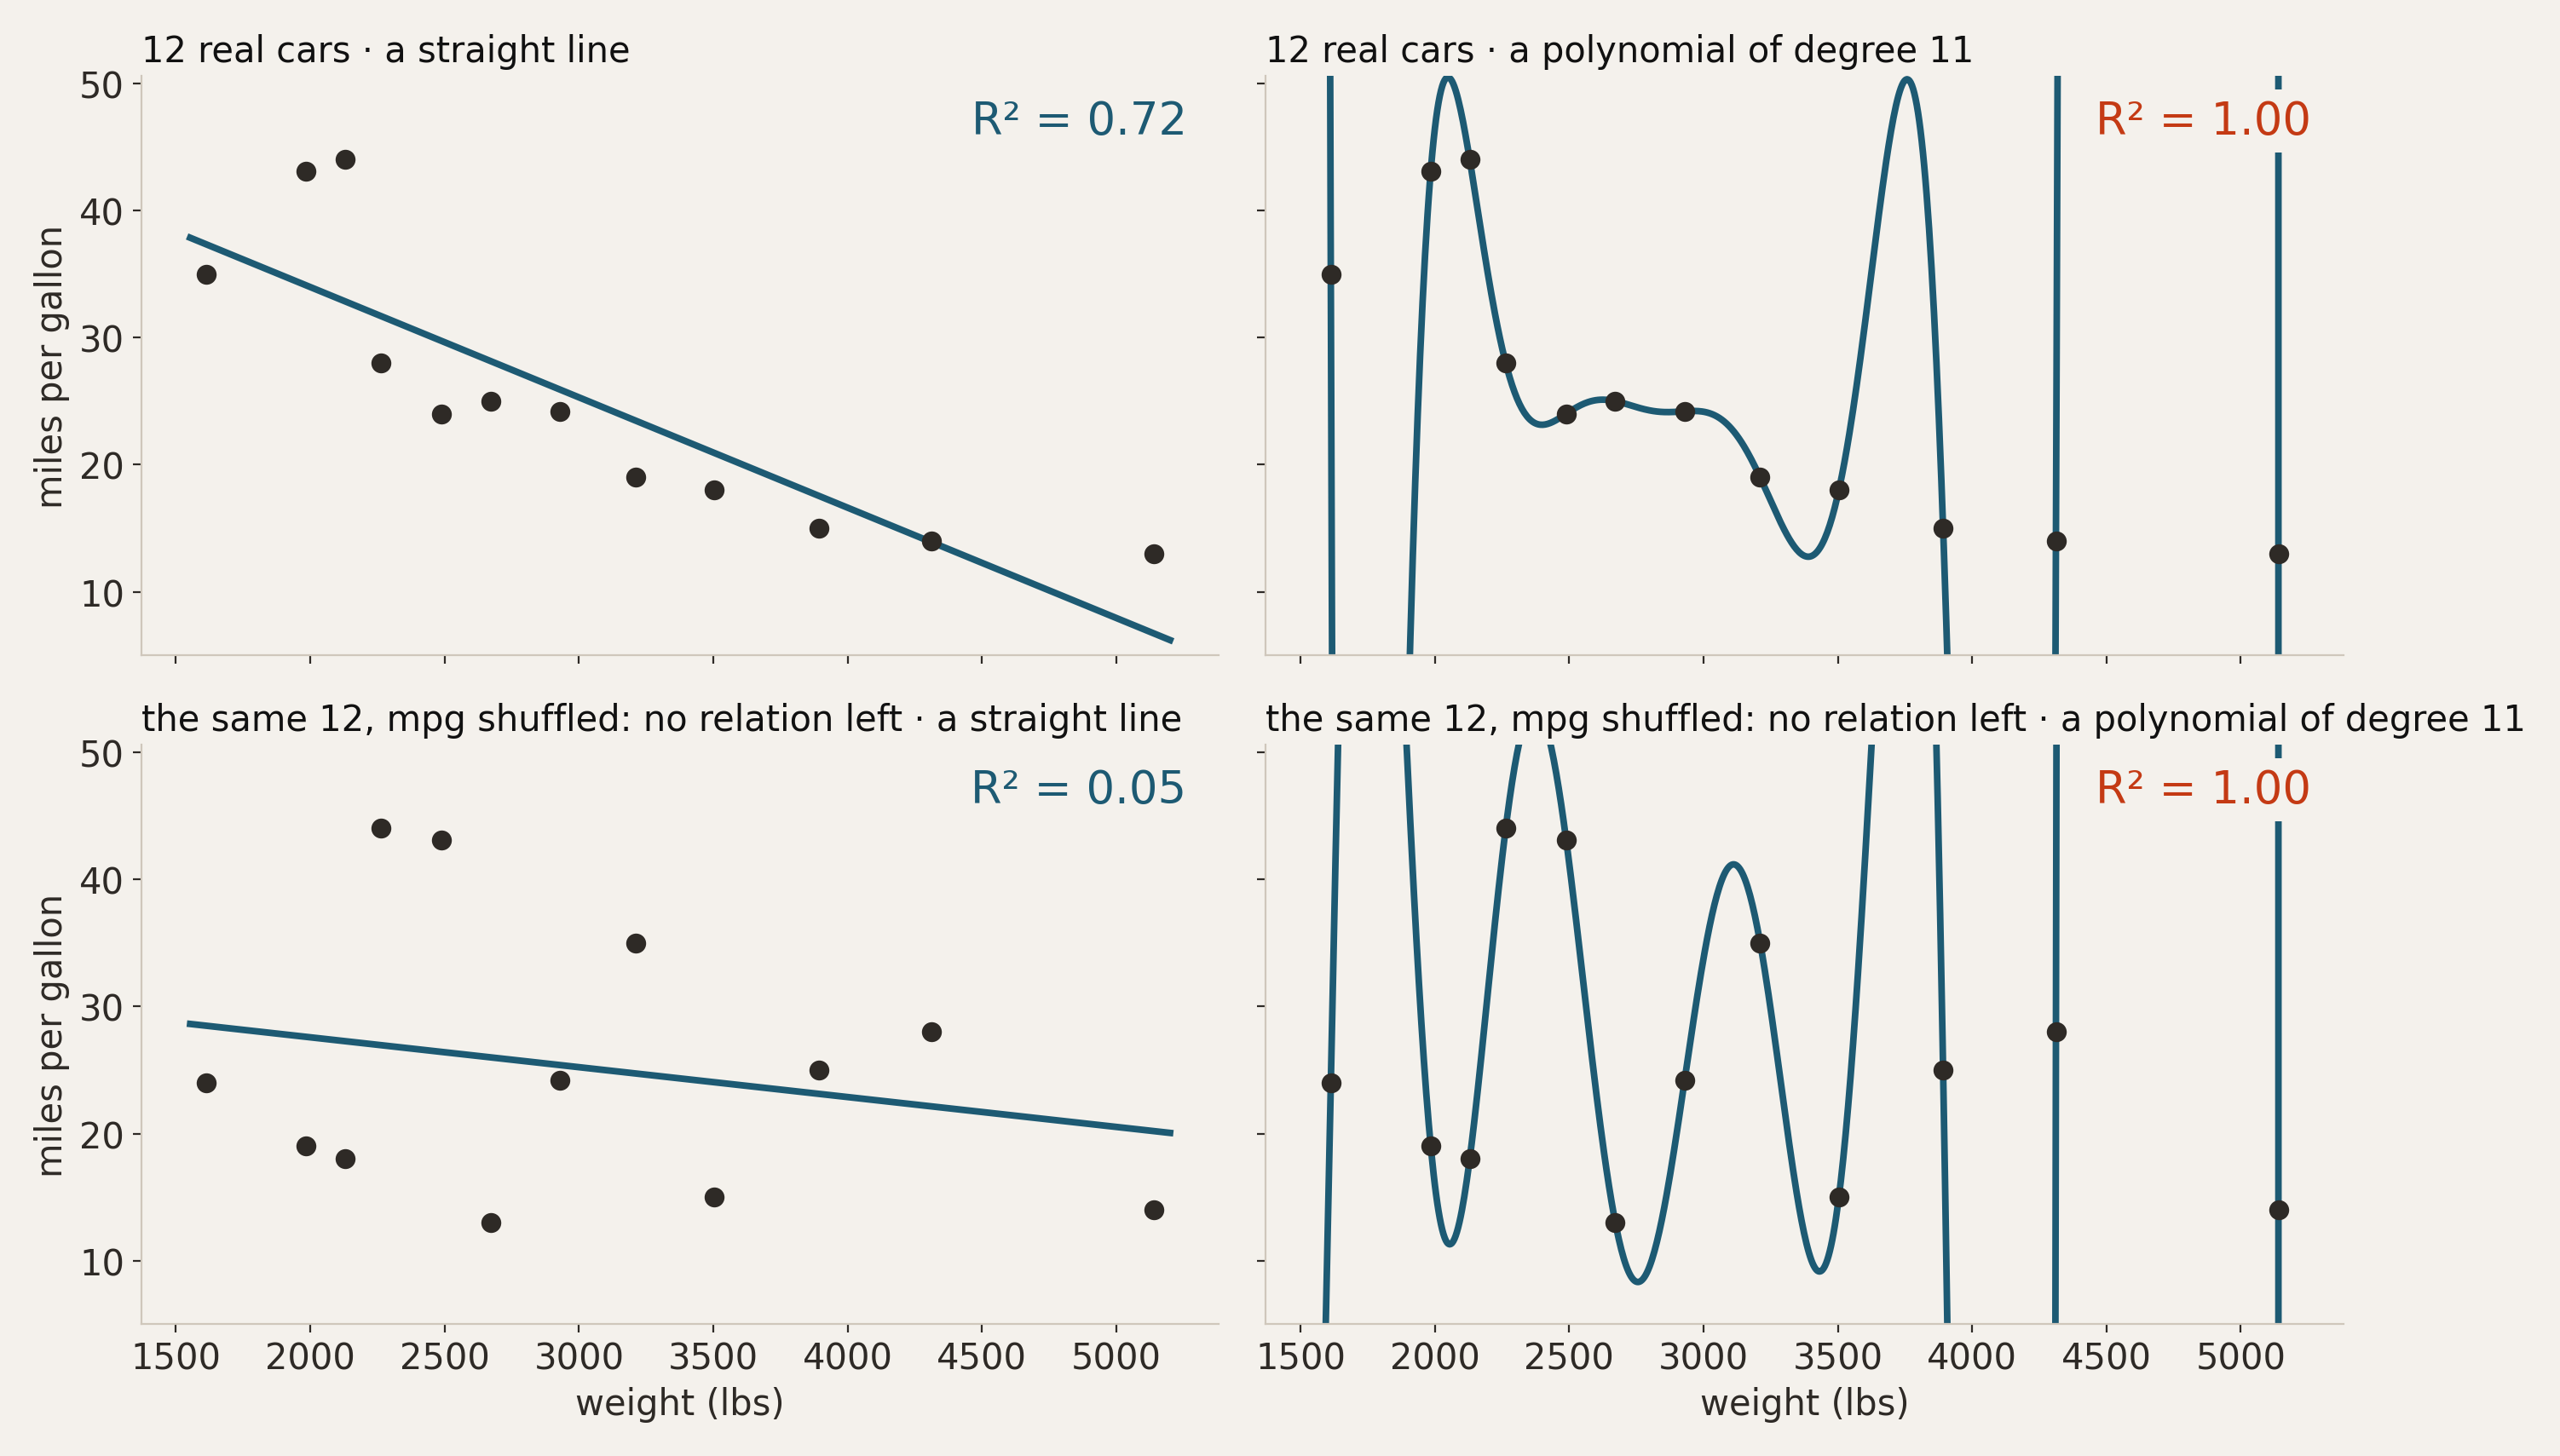
\includegraphics[width=\textwidth]{lesson5/flexible.png}
\caption{Top: twelve real cars. Bottom: the same cars with the fuel economy shuffled.}
\label{fig:flexible}
\end{figure}

Now shuffle the fuel economy values between the cars (bottom row). There is no relationship left; any pattern is chance, and a good model should break. The line does: $R^2 = 0.05$. Over $200$ shuffles its median is $0.05$, and $95\%$ of the shuffles stay below $0.28$. The polynomial scores a perfect $1.00$ again, on nonsense. You might think it is just so good that it always finds the pattern. It isn't; it is too flexible. A model that scores perfectly on real data and on nonsense cannot tell them apart, so its score is worthless. There is a paradox in this: because the line can fail, its $0.72$ tells you something about cars. This is the same shuffle as in lesson 4: ask what you would see if there were nothing there.

\subsubsection{Too simple, about right, too flexible}
Now test the three kinds of model on the $386$ cars they never saw, in the same weight range (figure~\ref{fig:newdata}).

\begin{figure}[H]
\centering
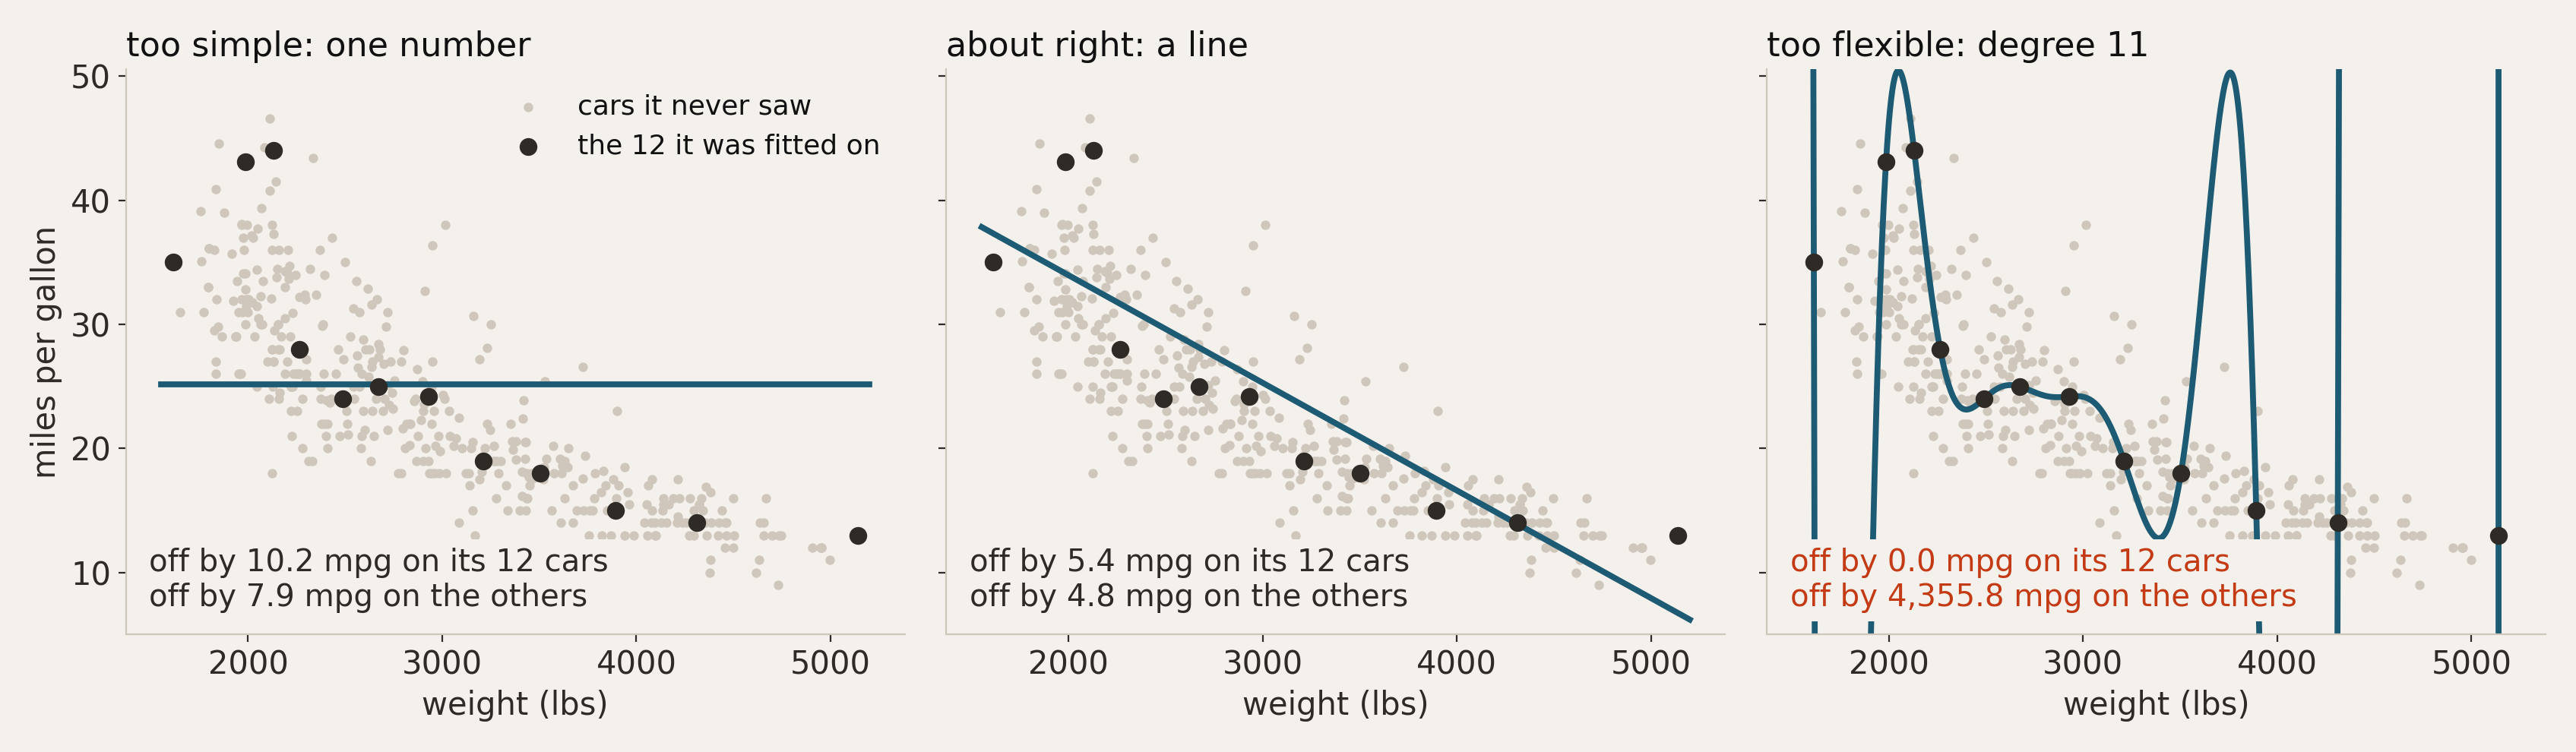
\includegraphics[width=\textwidth]{lesson5/new_data.png}
\caption{The same twelve cars, and 386 cars the models never saw.}
\label{fig:newdata}
\end{figure}

\begin{itemize}
\item \textbf{Too simple} (\emph{underfitting}): one number, the mean, for every car. It is about $10$ mpg off on its own twelve cars and about $8$ on the others. Bad everywhere, but at least honestly bad: it misses the pattern.
\item \textbf{About right}: a line, about $5$ mpg off on both. It is a bit wrong on its own cars and about as wrong on cars it has never seen. It learned something that carries over.
\item \textbf{Too flexible} (\emph{overfitting}): the polynomial is $0$ mpg off on its own twelve cars and on average more than $4{,}000$ mpg off on the others, because between the points it swings wherever it likes. It learned the twelve cars, not cars.
\end{itemize}

The tell-tale sign of overfitting is exactly this gap: very good on the data it saw, bad on new data. The trap is to look at the zero and think: look how good I am. You want a model that is about as wrong on new data as on old. Lesson 6 gives this its own machinery, with train and test sets; for now the intuition is enough.

\subsubsection{If you can't explain a number, don't report it}
This is a real report, handed in at another university of applied sciences, by a student who had worked on it for three months. The task was to predict the power draw of an engine. At the defence, two teachers and a half-hour presentation, the student showed six slides of MAPE formulas, all generated, and this table:

\begin{table}[H]
\centering
\begin{tabular}{@{}lrrr@{}}
\toprule
\textbf{Model} & \textbf{MAPE} & \textbf{MAE} & \textbf{RMSE} \\
\midrule
Random Forest & $4.78 \times 10^{13}$ & 0.89 & 2.5 \\
XGBoost & $5.48 \times 10^{13}$ & 0.53 & 1.3 \\
KNN regressor & $6.48 \times 10^{13}$ & 1.46 & 3.74 \\
\bottomrule
\end{tabular}
\end{table}

and the conclusion: ``These results suggest that the model is a robust and reliable tool for predicting power draw of the engine''. MAPE is the \emph{mean absolute percentage error}: on average, how many percent the prediction is off. A MAPE of $10^{13}$ means the model is off by ten trillion percent. If you understand what MAPE is, you cannot let that pass. So I asked: suppose I pay your salary with a model that has this MAPE. Are you worried? The student didn't really know. It means I might pay you one euro or ten billion euros, and I can't tell you which. Only then did it begin to dawn. The student failed.

The MAE column is no better. An MAE of $1.46$ means nothing until you compare it with a baseline error, for instance the error of always predicting the average. If that baseline is $0.001$, then $1.46$ is bizarrely high; if it is $100$, the model is excellent. Without the baseline nobody, the student included, can say whether the model is any good. (Why can MAPE reach $10^{13}$? It divides each error by the true value, so true values at or near zero blow it up. The student could not say that, and that is the point.)

In class someone asked whether there might have been an explanation for the number. Perhaps; but that is beside the point. The problem was that the student could not explain what was worrying about it, and the defence is far too late to discover that. If you present an employer with a robust model that is off by ten trillion percent and you don't see the problem, they will stop trusting the rest of your work too. It is like looking in your rear-view mirror on the motorway and seeing chunks of rubber flying and a shower of sparks behind you, because you are driving on the metal of your wheels, and concluding that your car might need some attention. That is not a maintenance issue. You stop. If you don't notice, you are a danger on the road.

So: use the tools, including an LLM, but every number on your slides is one you must be able to explain and defend. A number you can't explain is not a result.

\paragraph{When the simple model is the solution.}
A case from practice. At the start of the pandemic, the sales of Strepsils throat lozenges shot up and everything sold out. A complex sales model went completely off the rails trying to fit that peak. What worked was the opposite: a simple model with five or six sine waves for the rhythm of the year, which by construction could not follow the peak. The difference between that simple model and what actually happened we called the \emph{panic factor}: one parameter, fixed at zero up to the point where the simple model stopped working, and free after that. The model then had to put the whole COVID effect into that single parameter, so the effect was captured in one place. We then modelled three scenarios for the panic, that it would fade, disappear or stabilise, and gave the manager a knob to choose between them. That only worked because the model stayed simple enough to explain.

Is that an argument that simple models are usually right? Usually, yes; it is a trade-off. Simple models leave more on the table, but their inflexibility makes them reliable. There is also the opposite reflex: people so afraid of anything that cannot be explained that they stay simpler than necessary and reduce everything to a decision tree. In healthcare, for example, very complex models are used, because you can put far more information into them than any person can hold. That can be the right choice.

\againconcretely
A simple model can fail, and that is a signal you can use. Complex models find complex patterns, but you can't read them. Four shapes, each a sentence; a flexible model is not closer to the truth, it is closer to the noise; and a number you cannot explain does not belong in a report, however it was produced. Start simple. Add a term only when what is left over has a shape you recognise. If a model fails, that can be a very interesting signal about reality.

% ─────────────────────────────────────────────
\subsection{How do you build a model?}
\label{sec:building}
Every step goes the same way. You \emph{look}: plot the data and notice what is strange, such as noise, a delay or a difference in size. You \emph{think}: use what you know about the world, which is often not in the data at all. How does a disease progress? How does reporting work? When did the vaccine come? In your own chat this is knowledge like ``aunt Connie was single and bored that winter''. And you \emph{add}: turn each piece of reasoning into one step in the pipeline, or one term in the model. Then you look again.

The data are the public Dutch COVID figures: positive tests and deaths per day, from October 2020 to June 2021. The model in the end is small, but the way there is the lesson. Notebooks 05.3 and 05.4 follow the same path, and \texttt{scripts/covid\_pipeline.py} holds the whole loop as a script.

\subsubsection{\texorpdfstring{Step 0 · A running total. How many died per day?}{Step 0: A running total. How many died per day?}}
The data as it arrives. The Dutch figures give deaths as a running total: everyone who has died of COVID since February 2020, $6{,}419$ on 1 October 2020 and $17{,}632$ on 1 June 2021. That line can only go up, and the number that matters is hidden in how steep it is.

\begin{figure}[H]
\centering
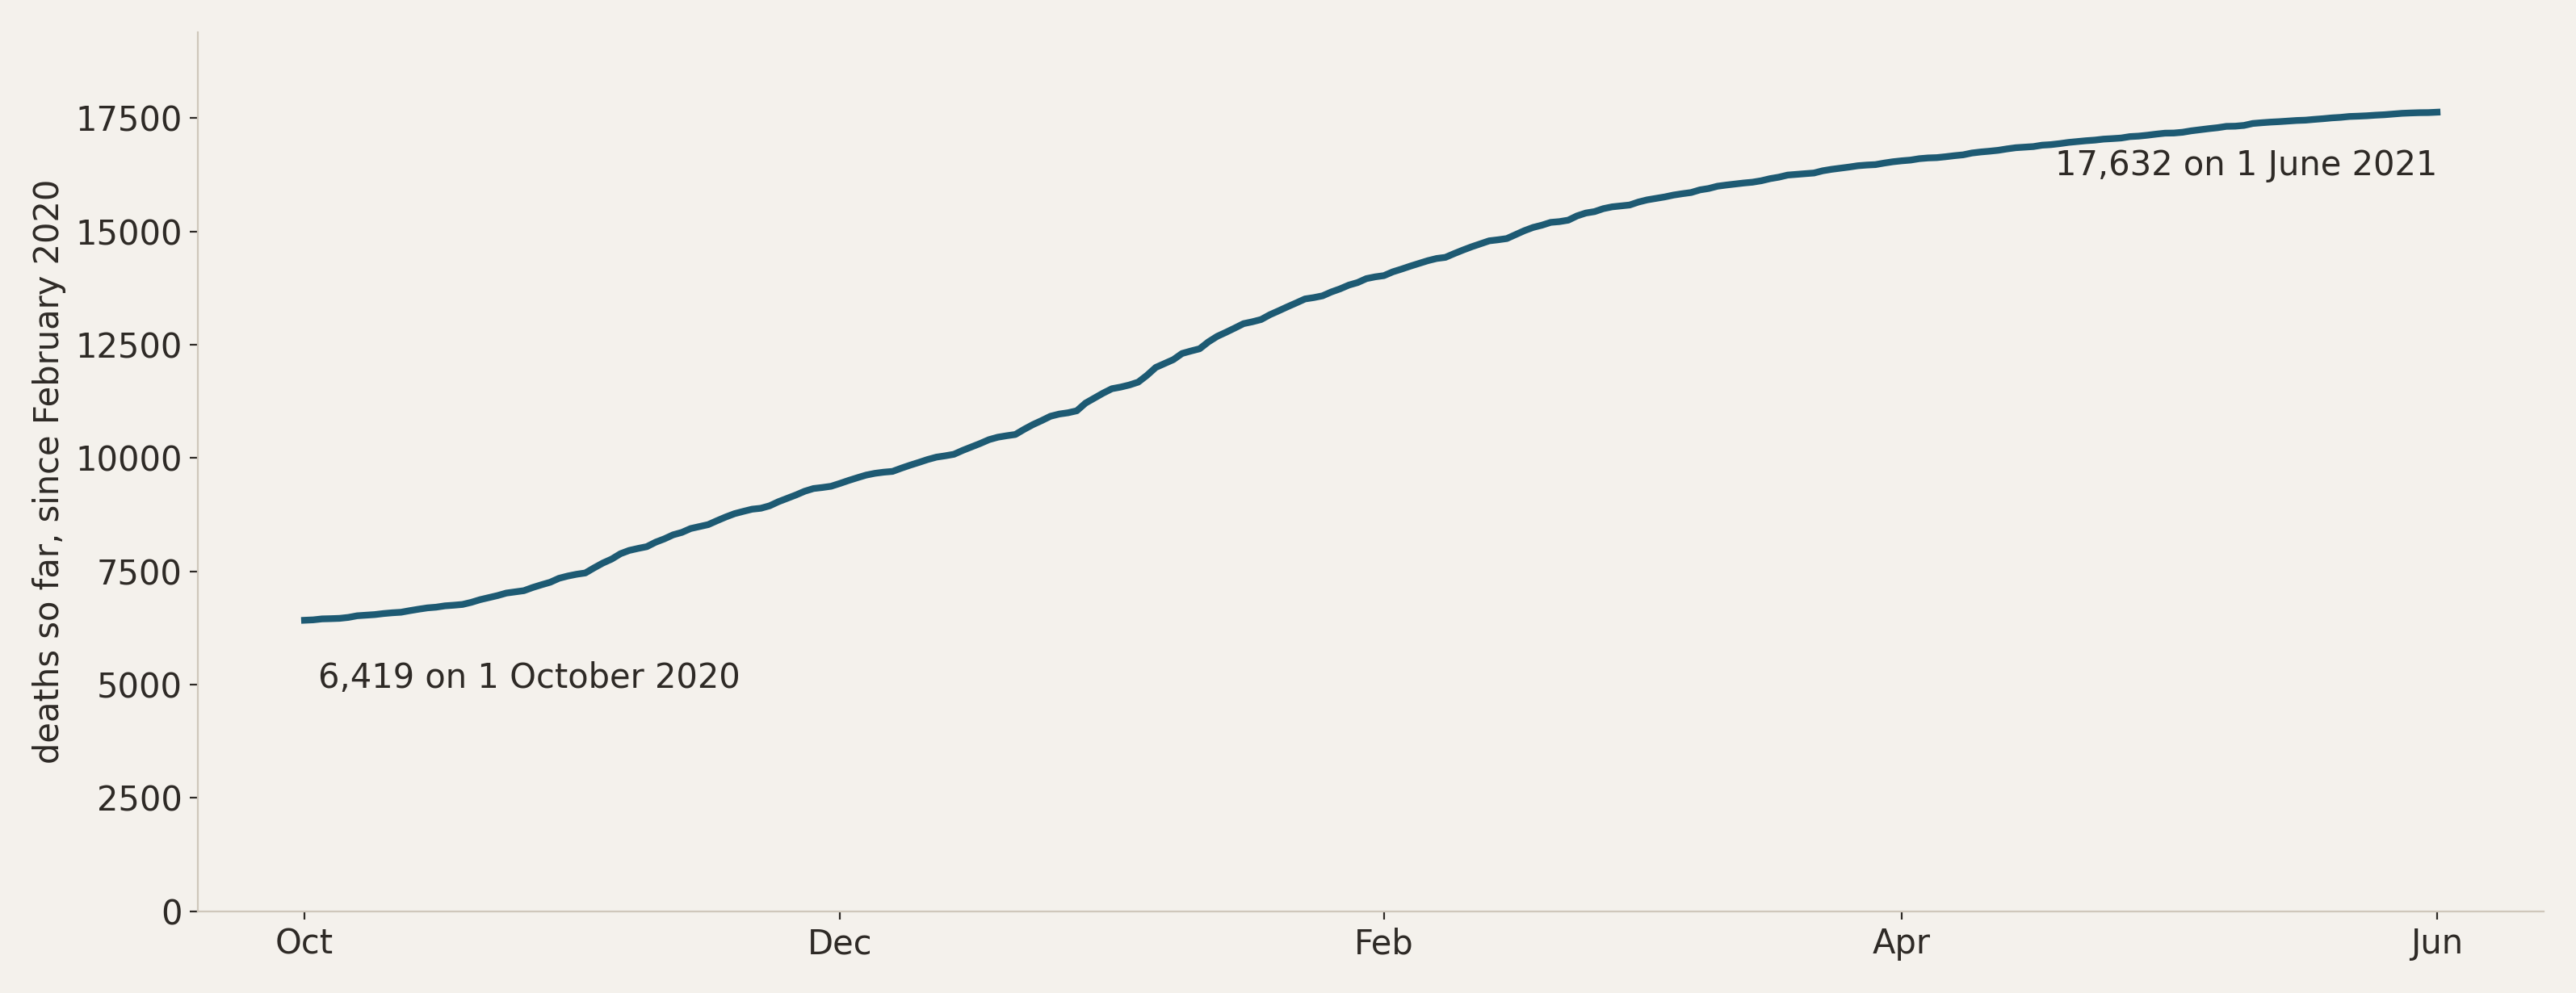
\includegraphics[width=\textwidth]{lesson5/covid_total.png}
\caption{The deaths as delivered: a running total.}
\label{fig:covid-total}
\end{figure}

How do you get the deaths per day out of this? Take the difference with the day before: deaths today $=$ total today $-$ total yesterday. In pandas that is \texttt{diff}, and in the pipeline it is the first step:
\begin{center}
\texttt{pipeline.add(DiffValues, column="deaths")}
\end{center}

\subsubsection{Preattentive processing: what do you see?}
In the first fraction of a second, before anyone reads an axis or a number, your visual system has already picked out what stands out: repetition, contrast, a pattern that keeps coming back. So look at the numbers exactly as reported, and ask yourself what you see before reading on.

\begin{figure}[H]
\centering
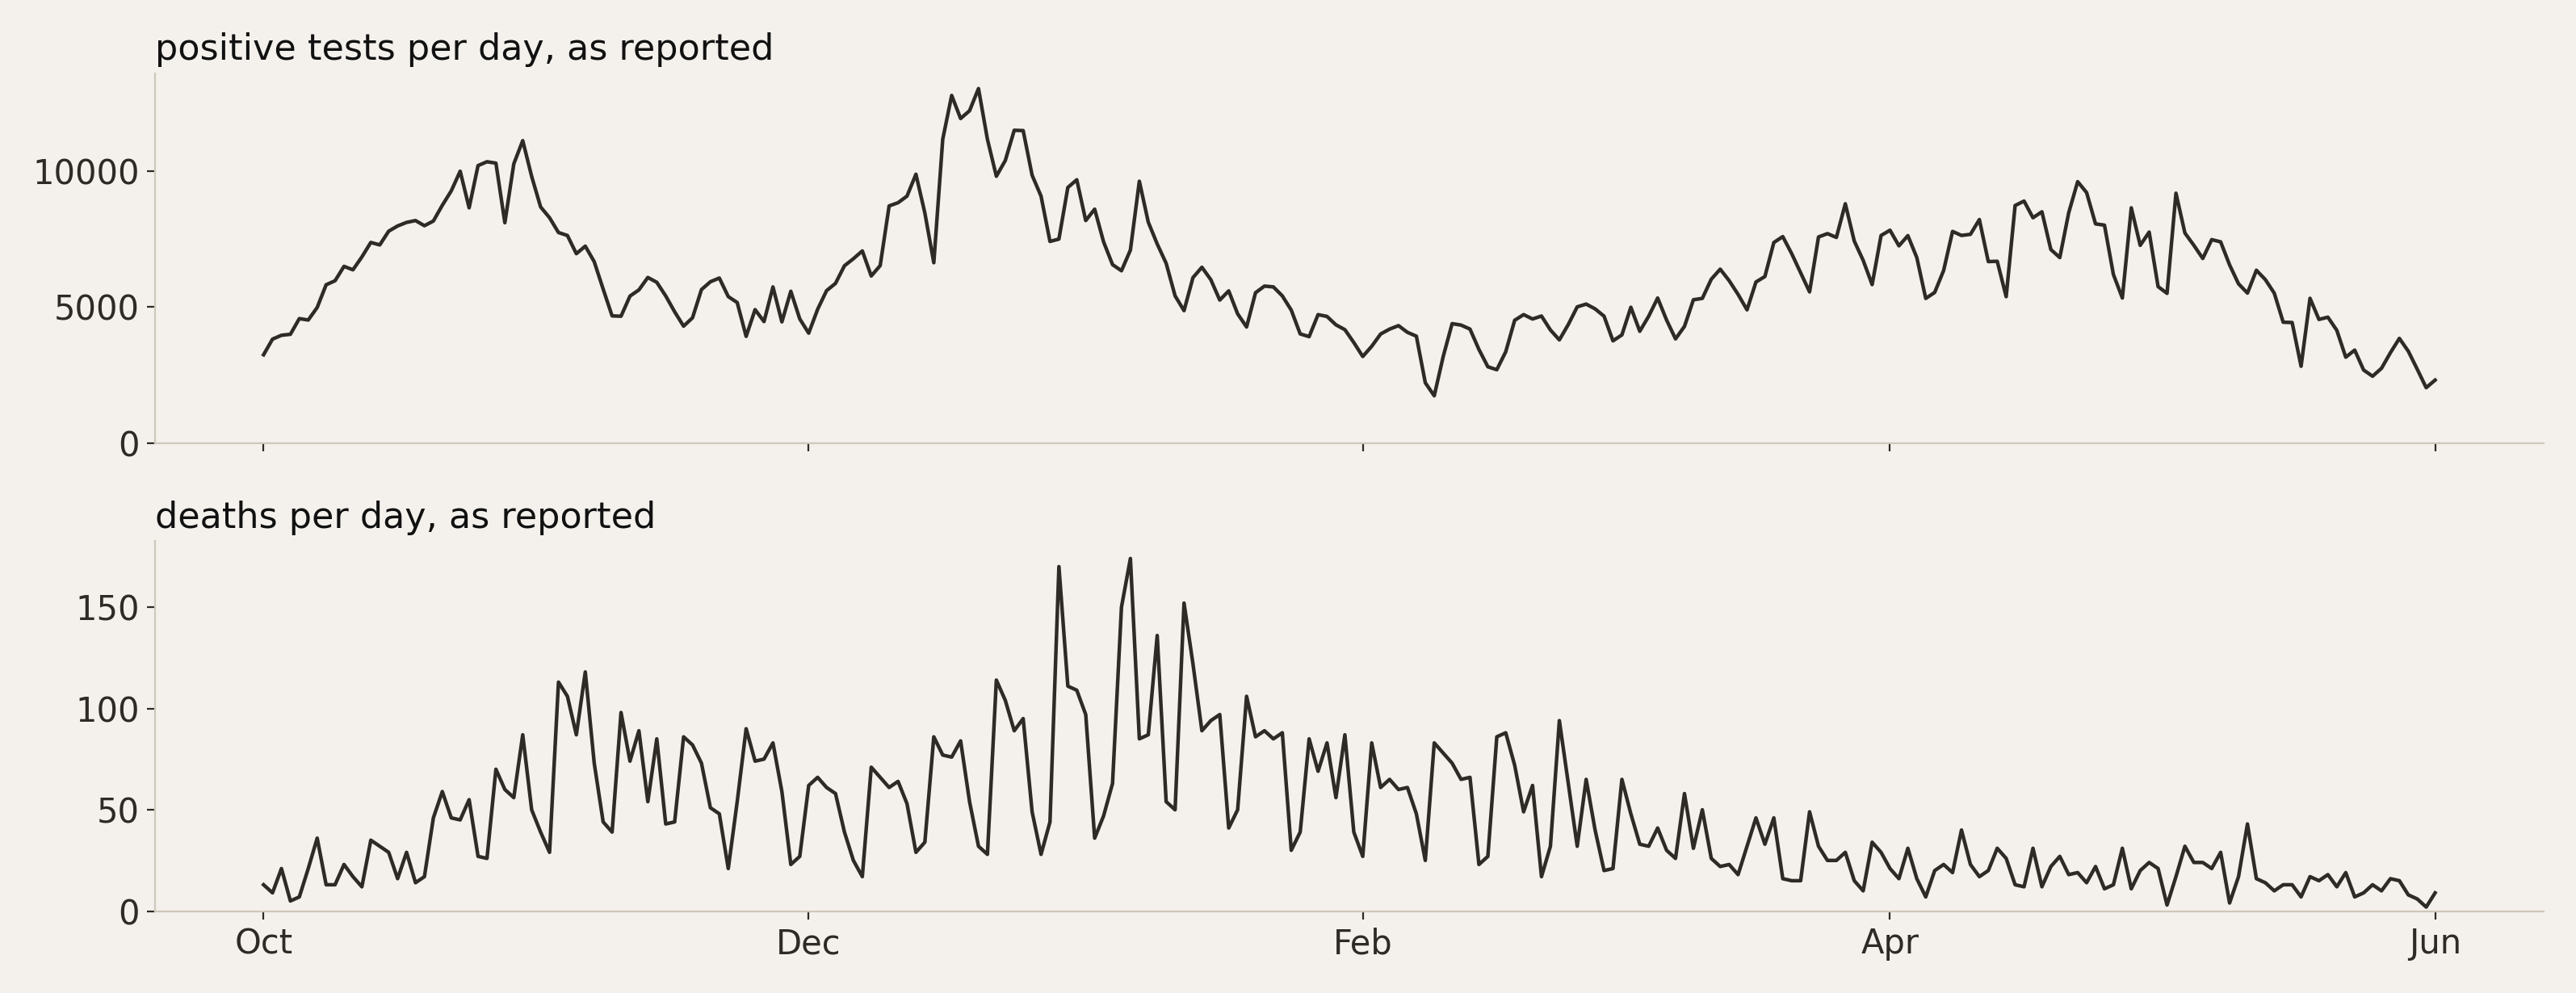
\includegraphics[width=\textwidth]{lesson5/covid_raw.png}
\caption{Positive tests and deaths per day, as reported.}
\label{fig:covid-raw}
\end{figure}

What jumps out first is the \emph{weekly cycle}, strongest in the deaths. On average about $25$ deaths are reported on Sundays and Mondays, and $67$ on Tuesdays. In class, the first explanations were the waves and the vaccine; those are the model, and we will come to them. The weekly rhythm is something else: people do not die less on Sundays. Registration waits for the weekend to end and catches up afterwards.

\subsubsection{\texorpdfstring{Step 1 · Too much noise: average over a week}{Step 1: Too much noise: average over a week}}
Should you remove the weekly cycle? That is a decision, and it depends on what you want to model. Here we are not interested in it: it tells us more about society than about the disease. Knowing that, the fix is obvious: average over seven days, so that every average contains each weekday exactly once.

\begin{figure}[H]
\centering
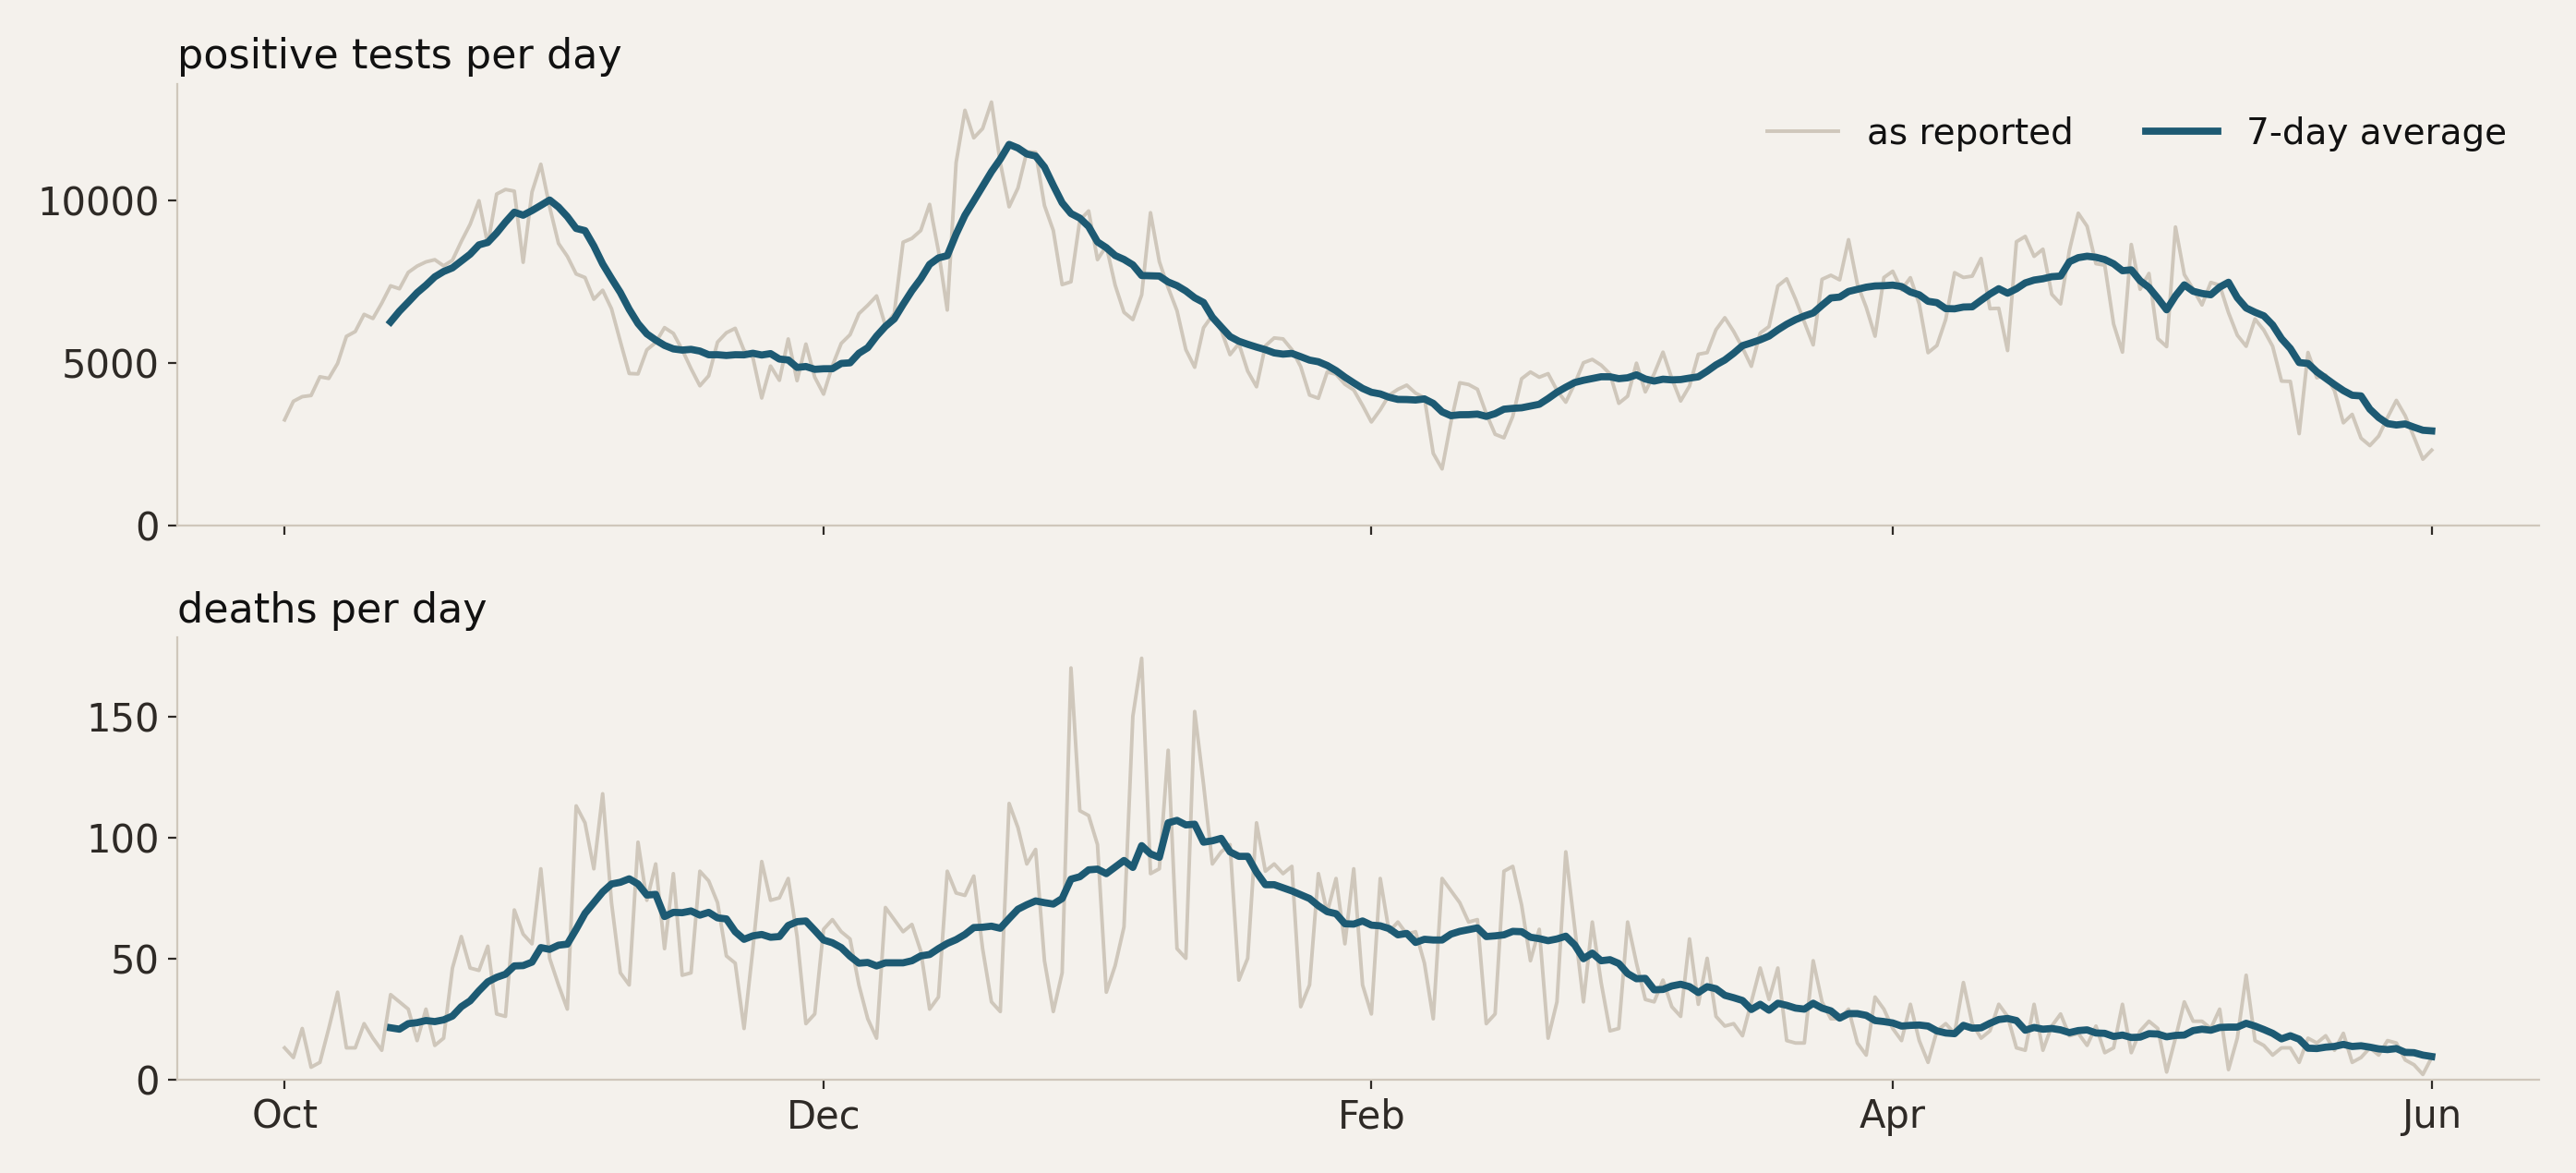
\includegraphics[width=\textwidth]{lesson5/covid_smooth.png}
\caption{Grey: the numbers as reported each day. Petrol: the average over the last seven days.}
\label{fig:covid-smooth}
\end{figure}

The weekly rhythm cancels out, and the course of the epidemic is left.
\begin{center}
\texttt{pipeline.add(RollingAvg, column="positivetests", window=7)}
\end{center}
and the same for the deaths.

\subsubsection{\texorpdfstring{Step 2 · Deaths come about two weeks after a positive test}{Step 2: Deaths come about two weeks after a positive test}}
With the weekly noise gone, something else becomes visible: the peaks in deaths come after the peaks in tests. You don't die on the day you test positive. Infection, illness, hospital, death: that usually takes about two weeks. That is knowledge from outside the data, from the medical literature (and at the time, from the news). So the deaths recorded fourteen days from now are the deaths of today's positive tests, and a model should pair them that way.

\begin{figure}[H]
\centering
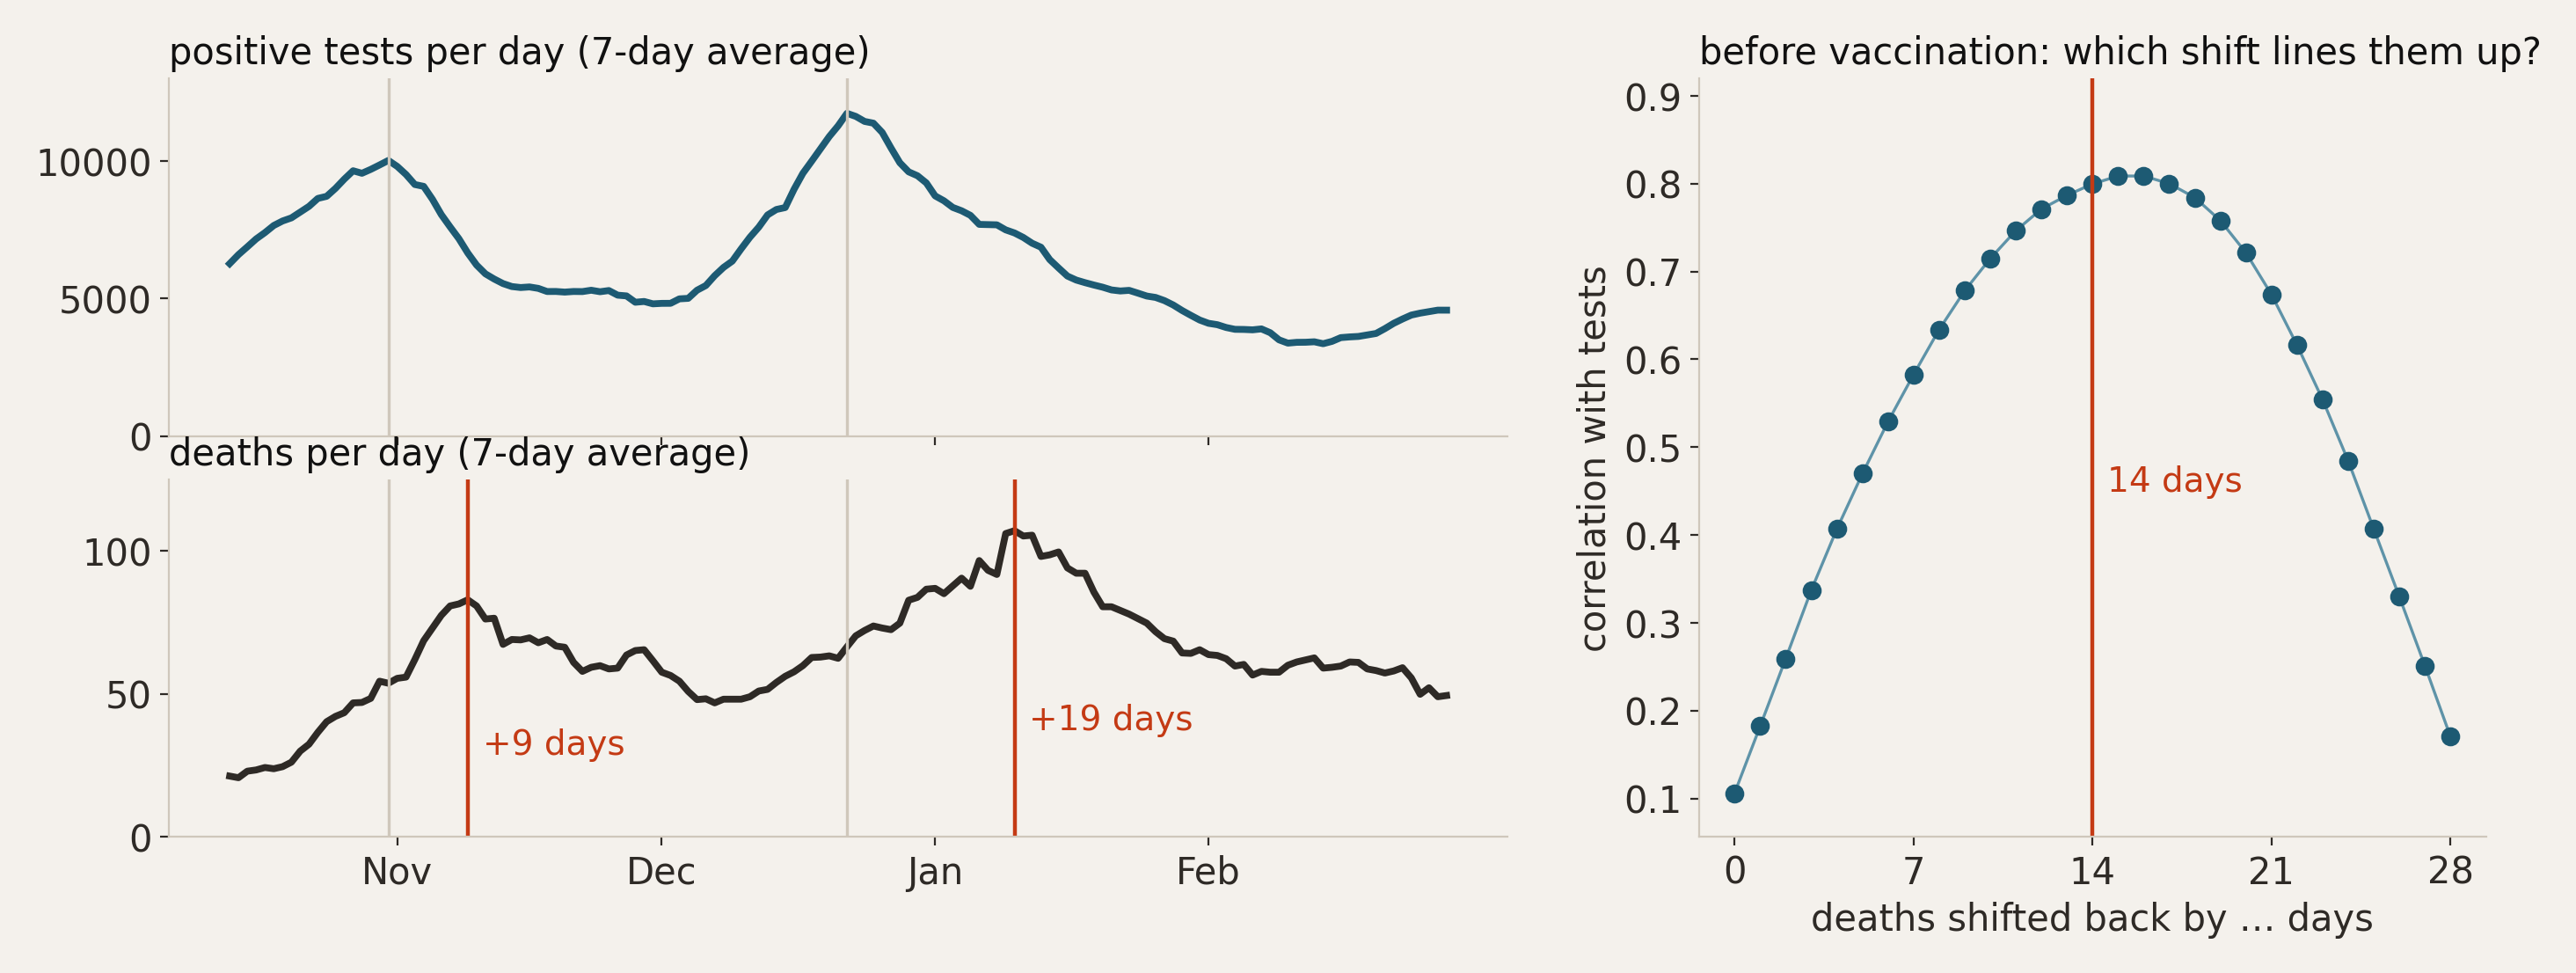
\includegraphics[width=\textwidth]{lesson5/covid_lag.png}
\caption{Left: tests peak, deaths follow. Right: the correlation between tests and deaths for every shift from 0 to 28 days, before vaccination.}
\label{fig:covid-lag}
\end{figure}

The left panel shows it with the naked eye: the deaths peak $9$ days after the tests in November, and $19$ days after them in January. Why the difference? In class we came up with several explanations: more testing discipline when people are worried, so infections are caught earlier; the most vulnerable people being infected and dying first; the holidays, when fewer people die and patients are kept alive until after New Year. We don't know. The right panel checks the two weeks: shift the deaths back by $0, 1, 2, \ldots, 28$ whole days and compute the correlation with the tests for each shift. The best shifts are around $14$ to $16$ days. The data agrees.

Why keep $14$, and not take $16$, which fits a little better? Because I don't know the mechanism behind $16$. It could be chance, Christmas, or any of the explanations above. If I tune the shift to this data, I artificially improve my model now and risk a worse fit in the future: I would be fitting noise. Note the order: the $14$ came from the literature, and the data confirmed it. Searching the data for the best lag and using that would be searching again, like the search for the switch day in lesson 4. If you want $15.6$ days, find it in the literature, or in data from other countries.

In the pipeline this is a shift of the deaths column, and it is also where the model starts:
\begin{center}
\texttt{pipeline.add(ShiftValues, column="deaths", period=-14)}
\end{center}
$$\text{deaths}(t) = a \cdot \text{tests}(t - 14).$$
What is $a$? ``The coefficient of the line'' is the mathematical answer. In normal language: if a hundred people test positive, $a$ is the share of them that dies two weeks later. Every term in a model should have an answer like that.

\subsubsection{\texorpdfstring{Step 3 · Tens against thousands: compare with z-scores}{Step 3: Tens against thousands: compare with z-scores}}
You want to see whether the two series have the same shape, but they live on different scales: thousands of positive tests a day, tens of deaths. On one axis the deaths are a flat line at the bottom.

\begin{figure}[H]
\centering
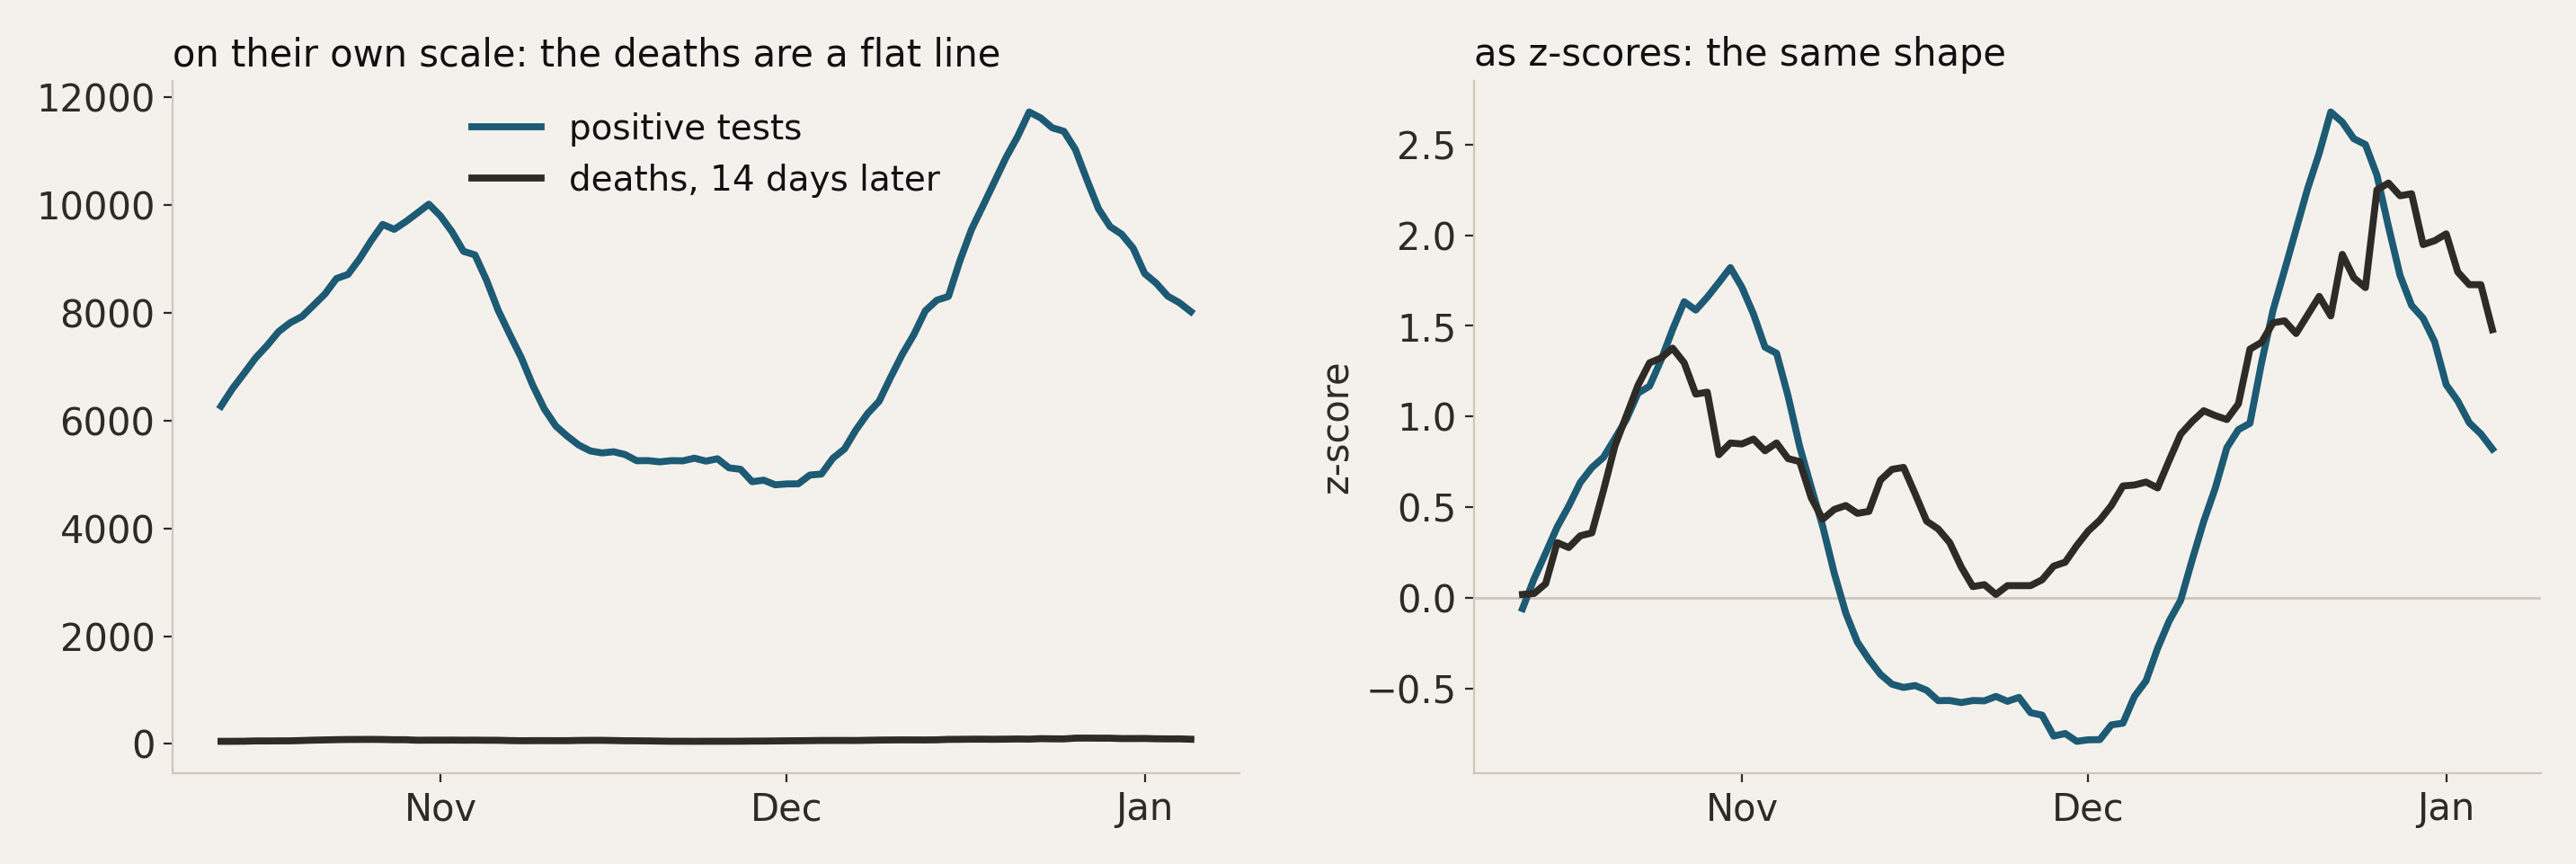
\includegraphics[width=\textwidth]{lesson5/covid_scale.png}
\caption{Left: tests and deaths on one axis. Right: both as z-scores, the deaths shifted two weeks back.}
\label{fig:covid-scale}
\end{figure}

A \emph{z-score} puts every series on the same scale: subtract its own mean and divide by its own standard deviation,
$$z = \frac{x - \text{mean}}{\text{sd}}.$$
Zero is an average day for that series; plus two is a very unusual one. In November there were two standard deviations more positive tests than average, and one and a half standard deviations more deaths. As z-scores, the deaths two weeks later follow the shape of the tests. You know z-scores already; the point here is why you use one: to compare shapes, not sizes.
\begin{center}
\texttt{pipeline.add(ZScaler, column="positivetests", rename=True)}
\end{center}
Be careful not to put the z-scores into the model. You could, but then $a$ would no longer be a share of people who die; it would become something like $0.8$, meaning nothing you can say out loud, and you would have to calculate back. The z-scores are for looking; the model uses the counts.

\subsubsection{\texorpdfstring{Step 4 · Add what you know: vaccination started on 6 January}{Step 4: Add what you know: vaccination started on 6 January}}
Over the whole window the picture changes. Until January the two curves move together; from February they part. The tests rise again in spring, the deaths keep falling.

\begin{figure}[H]
\centering
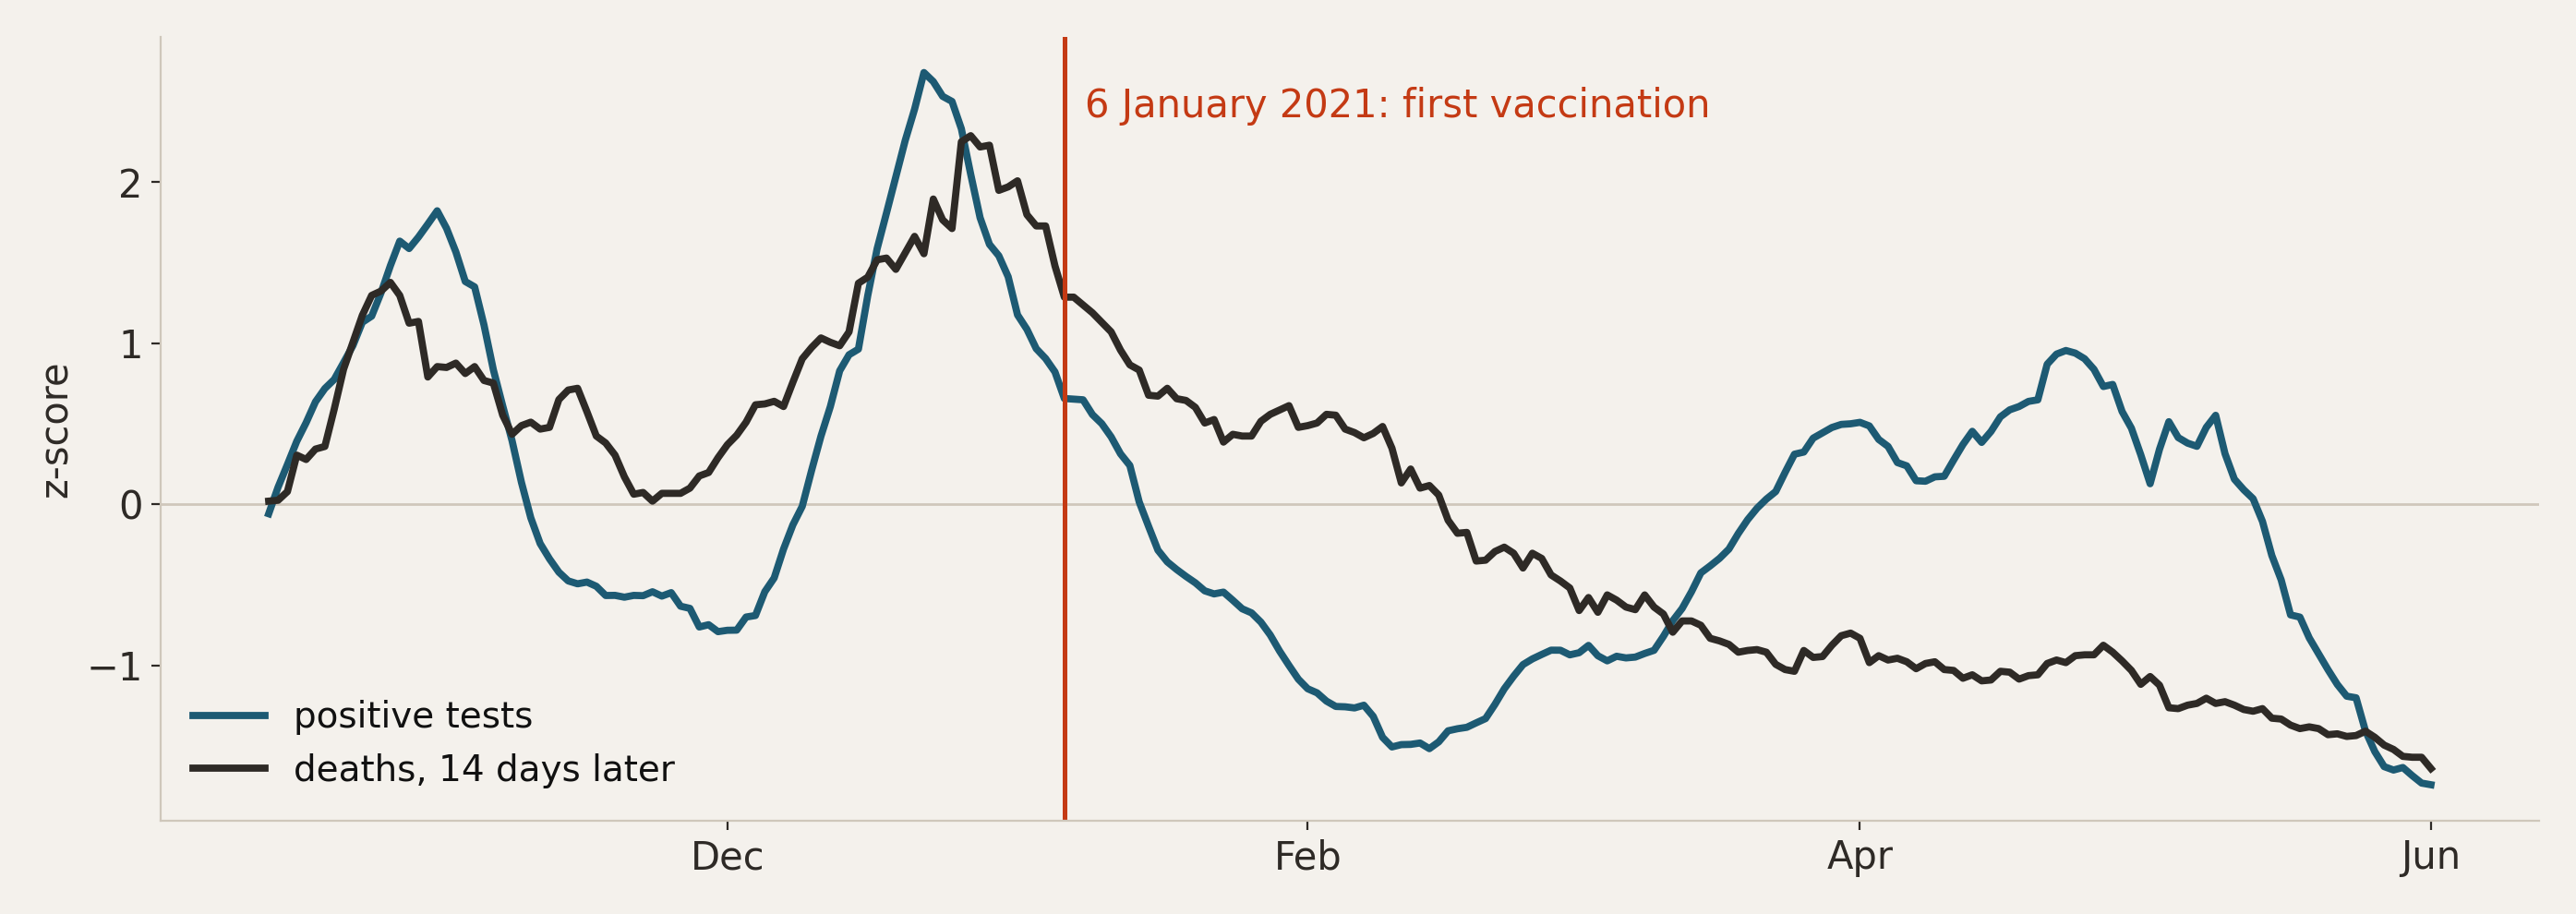
\includegraphics[width=\textwidth]{lesson5/covid_event.png}
\caption{The whole window as z-scores, with the first vaccination in the Netherlands.}
\label{fig:covid-event}
\end{figure}

The data doesn't say why; it has no column for it. You know something it doesn't: the first vaccination in the Netherlands was given on 6 January 2021. I didn't get that date from the data but from the news. People who are vaccinated still get infected; they just die much less often. (Could it be false positive tests? Possibly, but tests are fairly reliable, and you would also have to explain why they gave few false positives before January and many after.)

The date does two things. It tells us where the relationship between tests and deaths is likely to hold, before vaccination, so that is where we fit the first model. And it gives us a guess for where something might change. The pipeline's \texttt{SelectDataRange} makes the same kind of decision for the whole study: which months to look at, here 1 October 2020 to 1 June 2021.

\subsubsection{Add b: the deaths the tests don't explain}
A line is $a \cdot x + b$. Instead of adding a $b$ because lines have one, ask what it would mean here. Fit the model from step 2 on the $85$ days before vaccination, and the line has to go through zero: $a = 0.0090$, the dashed line in figure~\ref{fig:covid-fit}. Now add a constant:
$$\text{deaths}(t) = a \cdot \text{tests}(t - 14) + b.$$

\begin{figure}[H]
\centering
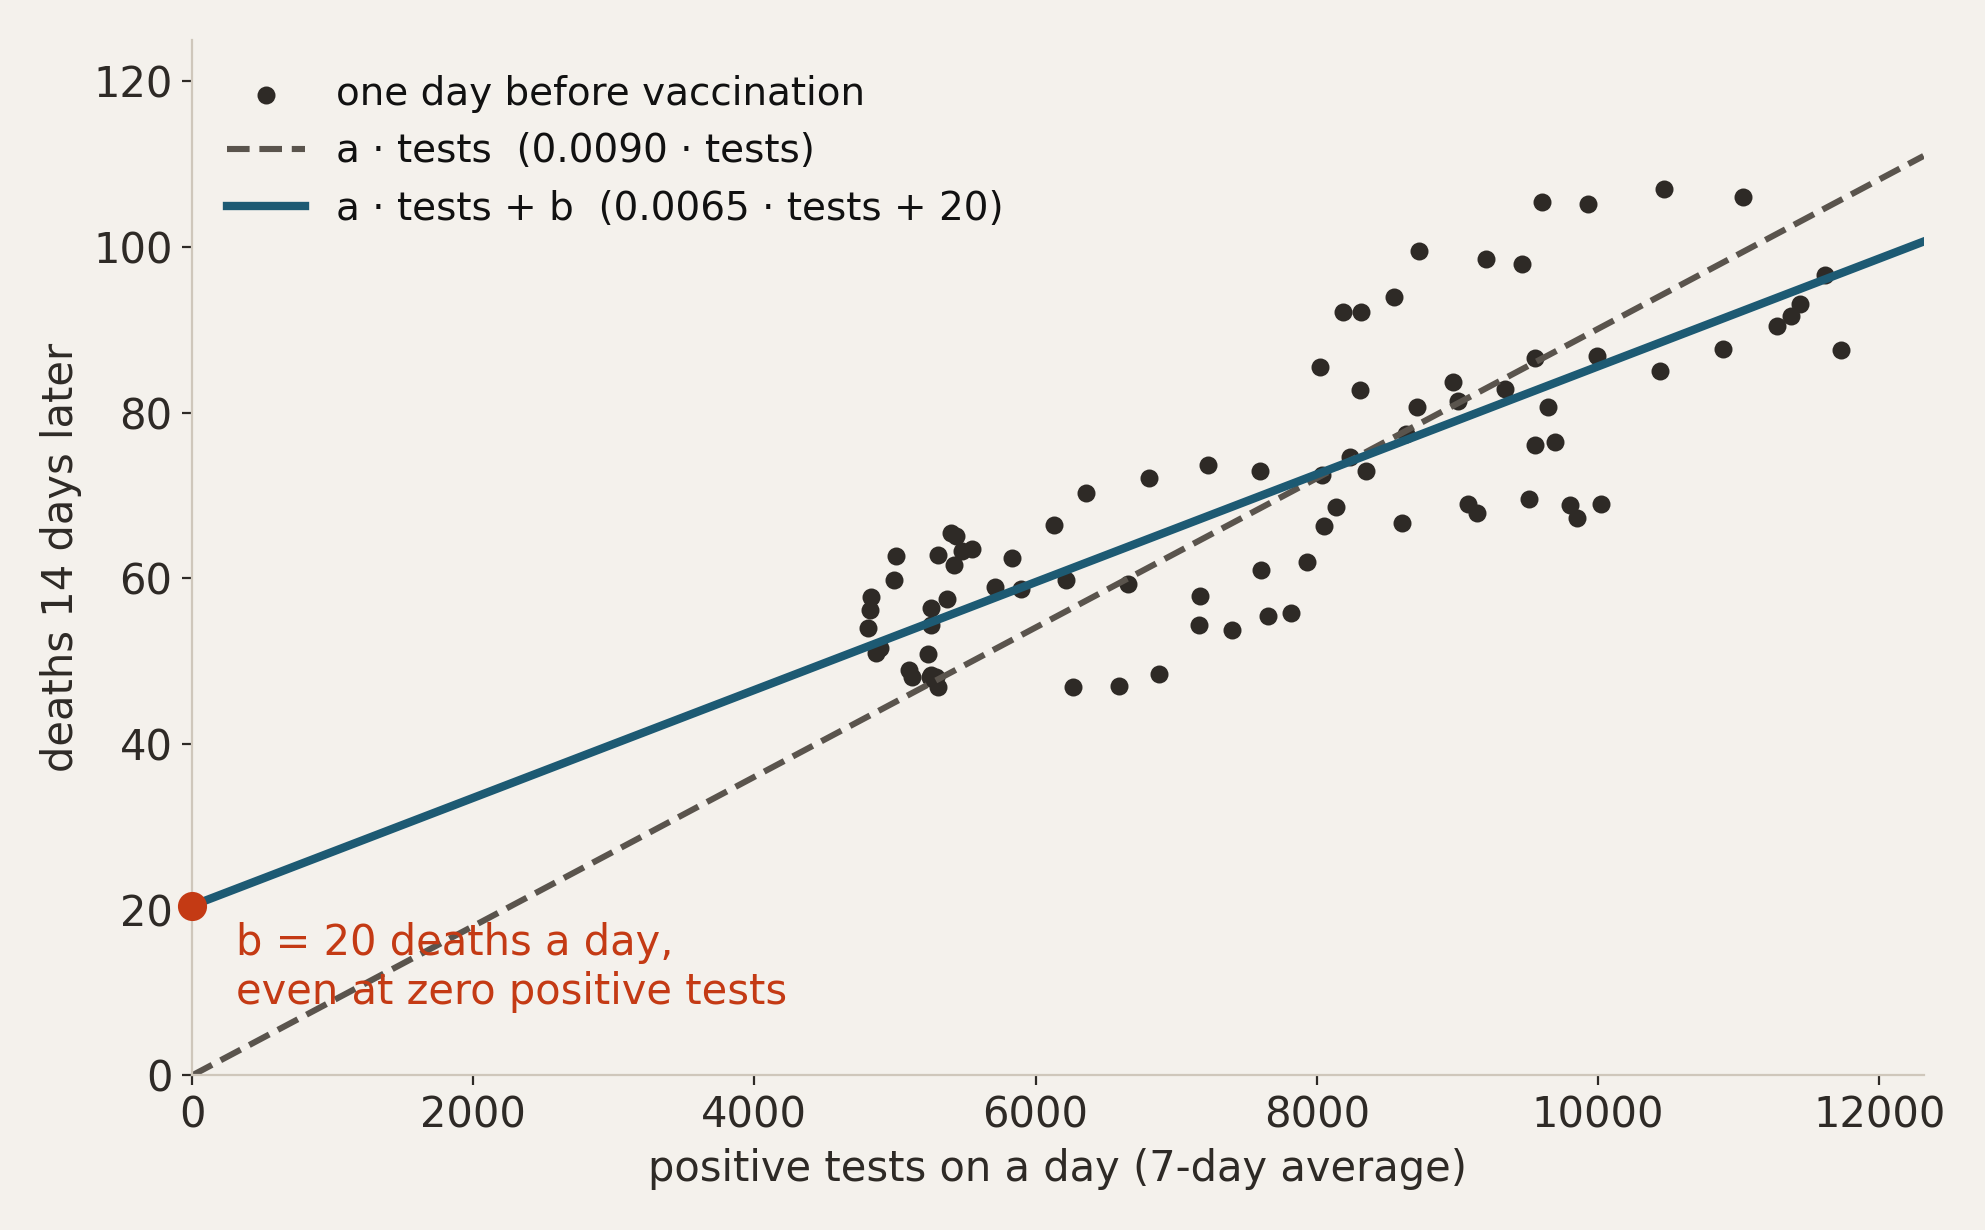
\includegraphics[width=0.65\textwidth]{lesson5/covid_fit.png}
\caption{The 85 days before vaccination, with and without $b$.}
\label{fig:covid-fit}
\end{figure}

The fit puts $a$ at $0.0065$: of every hundred positive tests, $0.65$ end in death two weeks later. And $b$ at about $20$ deaths a day, even at zero positive tests. Those are deaths that happen whatever the number of tests: people who were never tested, or people who die \emph{with} COVID rather than \emph{of} it, because they were positive and old. With $b$ the line is closer to the points: the mean squared error drops from $127$ to $99$. And $b$ gives the model room for deaths that stay when $a$ changes, which we will need shortly. One caution: no day in this window had fewer than about $4{,}800$ positive tests, so $b$ is where the line meets zero tests, an extrapolation. Read it as the deaths the tests don't account for, not as a measured count.

\subsubsection{\texorpdfstring{Step 5 · Say how wrong the model is allowed to be}{Step 5: Say how wrong the model is allowed to be}}
The last term is the noise:
$$\text{deaths}(t) = a \cdot \text{tests}(t - 14) + b + \varepsilon, \qquad \varepsilon \sim \mathcal{N}(0, \sigma).$$
Writing down $\varepsilon$ is a claim: everything the line doesn't explain (lockdowns, demonstrations, Christmas, new variants, people having coffee together anyway) is treated as chance, normally distributed around zero. Here $\sigma$ is about $10$ deaths a day. That is modelling the uncertainty: the model says not only what it expects, but how far off it is allowed to be.

\begin{figure}[H]
\centering
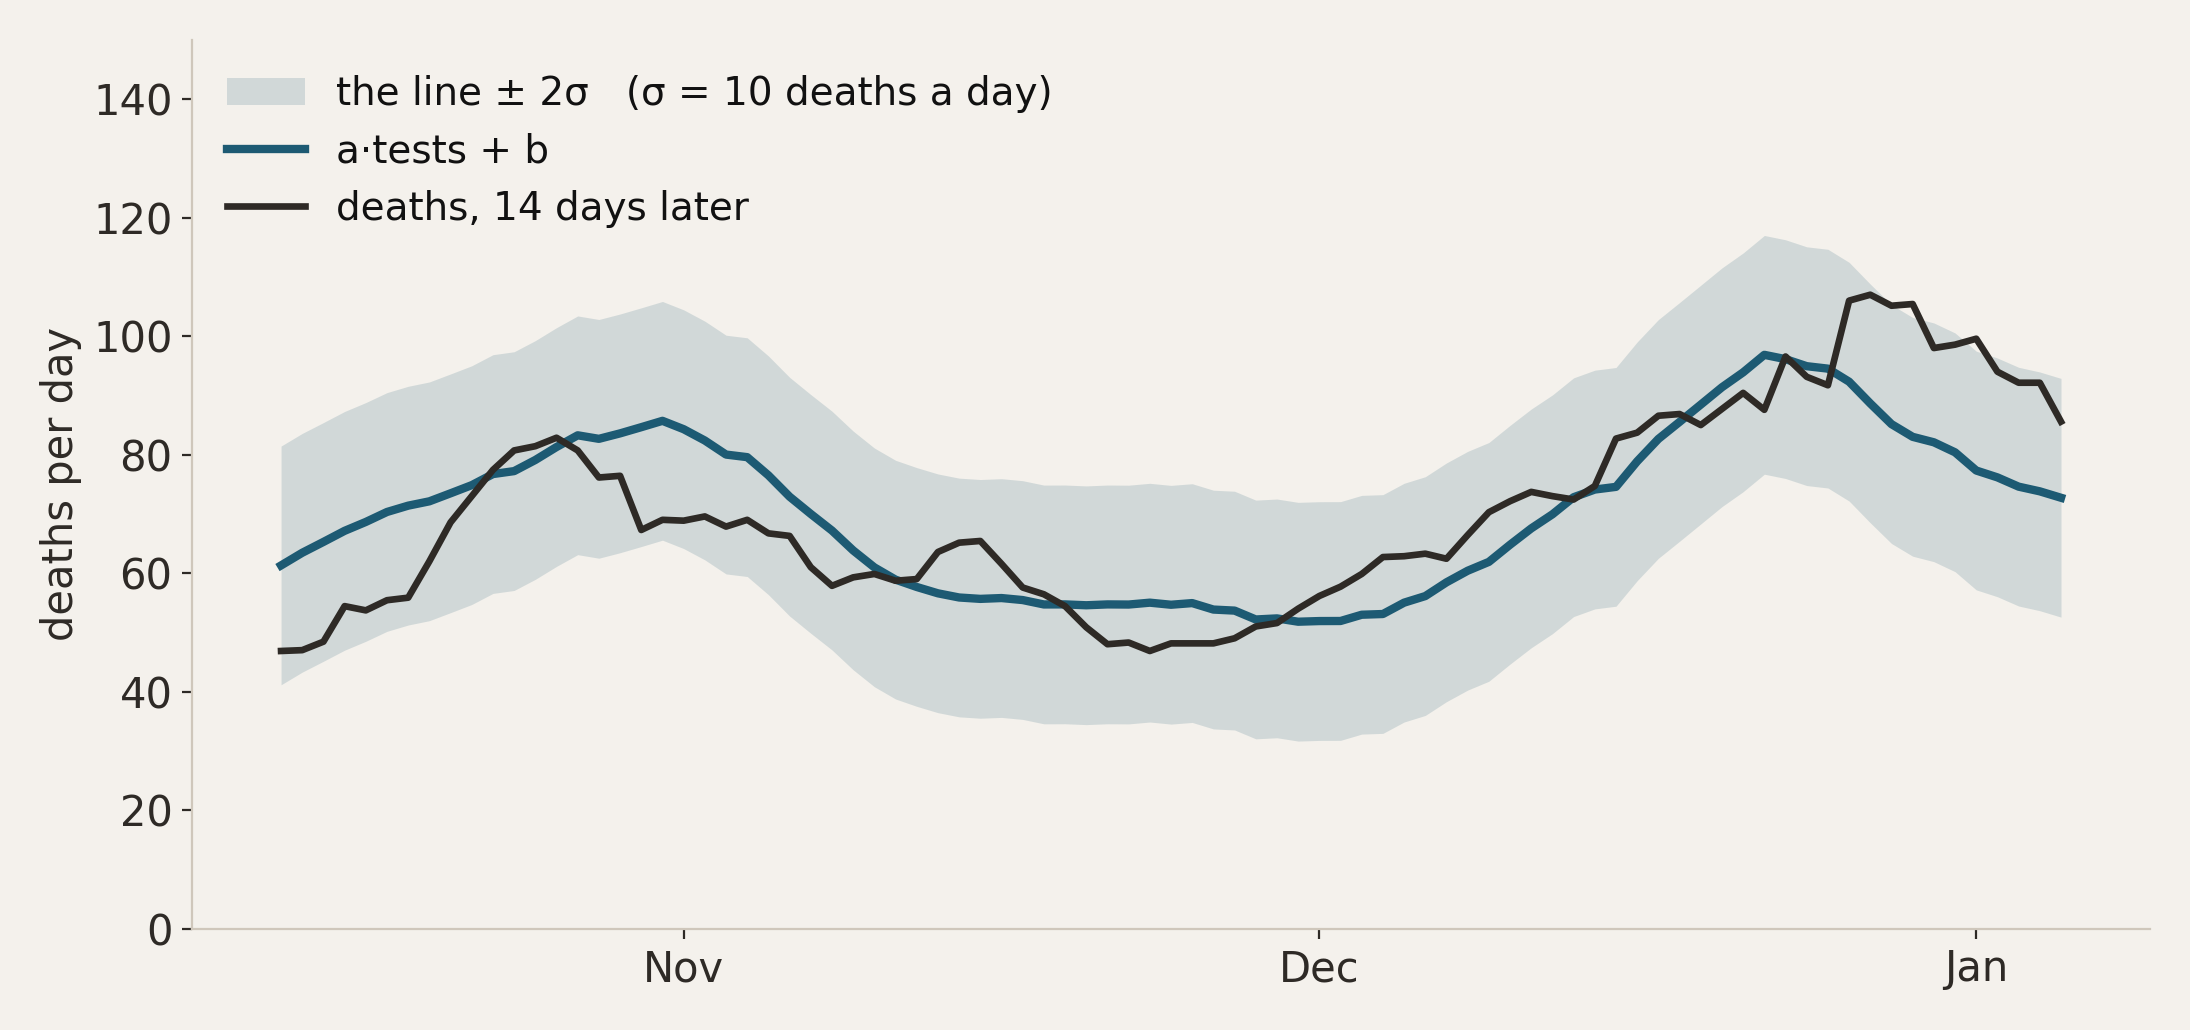
\includegraphics[width=0.75\textwidth]{lesson5/covid_band.png}
\caption{The model with a band of $\pm 2\sigma$, October 2020 to 5 January 2021.}
\label{fig:covid-band}
\end{figure}

How do you find $\varepsilon$? You know the deaths and the tests; you don't know $a$, $b$ or $\varepsilon$. But you can fit $a$ and $b$, and then what is left is $\varepsilon$:
$$\varepsilon = \text{deaths}(t) - \big(a \cdot \text{tests}(t - 14) + b\big).$$
That is the residual from lesson 4. Plus or minus two $\sigma$ should hold about $95\%$ of the days; it holds $98\%$ of the $85$ days before vaccination. And because $\varepsilon$ is a claim, it can be checked: if the errors stop looking like chance, the model is missing something. goad's \texttt{DistributionFitter} is the tool for that check. You could argue that the bump around Christmas is not chance; then add Christmas to the model. Treating it as noise is a choice, and it is a choice you make out loud.

\subsubsection{Every step of reasoning becomes a line of code}
This is the part to remember. Every piece of reasoning from the last five steps ended up in one of two places: the pipeline that prepares the data, or the formula of the model.

\begin{table}[H]
\centering
\begin{tabularx}{\textwidth}{@{}l X@{}}
\toprule
\textbf{Pipeline step} & \textbf{The reasoning behind it} \\
\midrule
\texttt{DiffValues} & A running total of deaths; you want deaths per day. \\
\texttt{ShiftValues(-14)} & Deaths come about two weeks after a test: the literature. \\
\texttt{SelectDataRange} & The months you want to study. \\
\texttt{RollingAvg(7)} & Weekends are society, not disease. \\
\texttt{ZScaler} & Tens against thousands: compare the shapes. \\
\bottomrule
\end{tabularx}
\caption{The pipeline, \texttt{CovidDataProcessor}, and the reasoning behind each step.}
\label{tab:covid-pipeline}
\end{table}

In the model, $\text{tests}(t - 14)$ is the same two weeks as \texttt{ShiftValues(-14)}, now in the formula. The parameters $a$ and $b$ are fitted on the days before 6 January, a date from outside the data. And $\varepsilon$ says that what the line can't explain is chance, which is itself a claim the residual can check. A \texttt{DataConfig} holds the $14$, the $7$ and the window, so every decision has one place where it lives. Nothing here came out of the data by itself. Each step is a decision you can explain and point at, and that is why a pipeline is built from named steps instead of one long chain of pandas.

\subsubsection{Previous lesson: the residual shows what the line misses}
Now take the line exactly as fitted before vaccination, with the same $a$ and $b$, and run it over every day up to June. Nothing in it knows what month it is.

\begin{figure}[H]
\centering
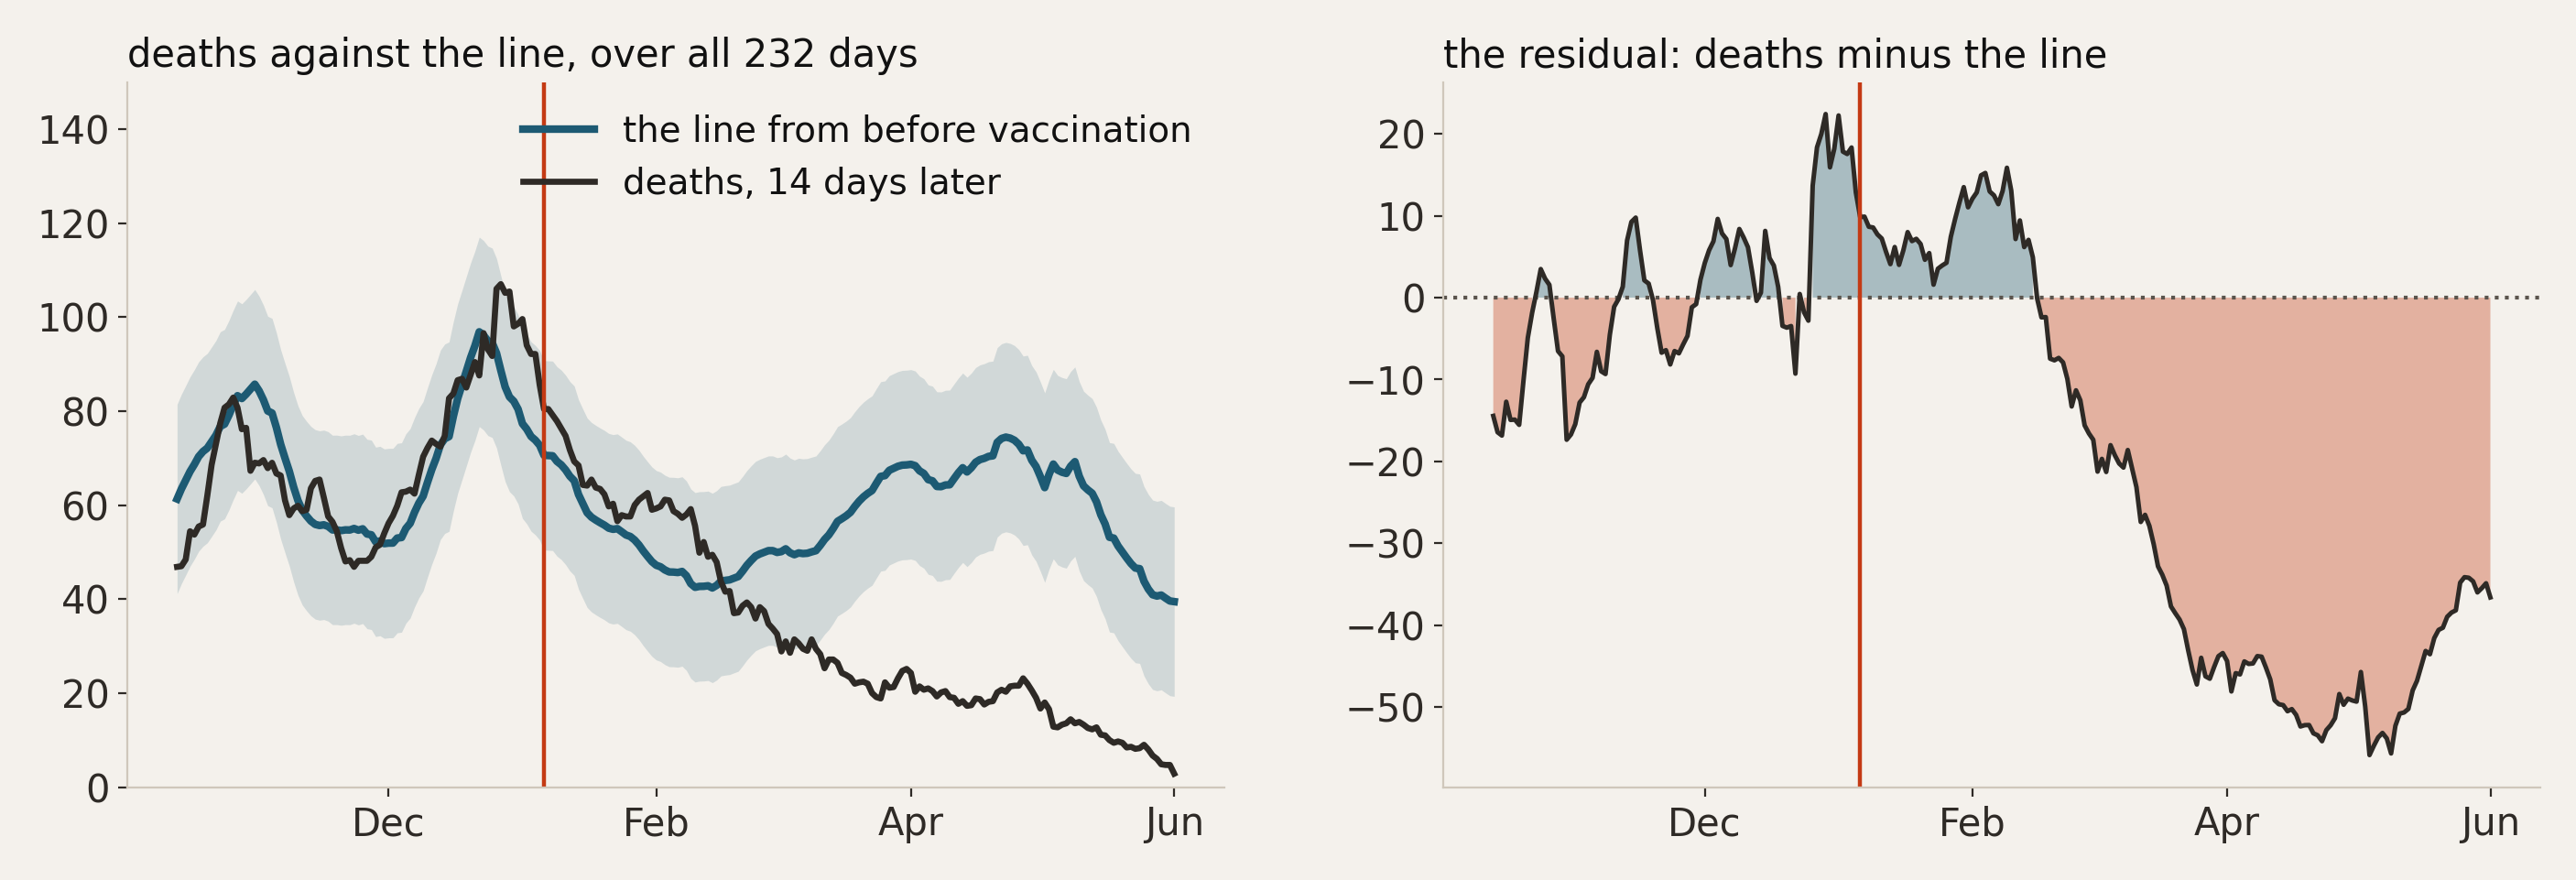
\includegraphics[width=\textwidth]{lesson5/covid_residual.png}
\caption{Left: the line from before 6 January, over all 232 days. Right: the residual.}
\label{fig:covid-residual}
\end{figure}

Until January the deaths stay inside the band. From February they drop below it and never come back: $60\%$ of the days after 6 January fall below the band. Even what we modelled as noise no longer covers it. The residual is below zero from 16 February to the end, at its worst about fifty deaths a day. Up to January you could still say: sometimes a bit higher, sometimes a bit lower, all chance. After that it is no longer chance. The errors have a shape, a long run in one direction. One fixed share of tests ending in death no longer works. Something changed the ratio, and the residual says roughly when. How do you put that into the model?

\subsubsection{How do you model a vaccine? Look at the ratio}
Not with a separate line per month, and not with a polynomial in time that bends until the residual is flat; that would match the picture and explain nothing. This is the moment many students say: my linear model and my random forest don't work, so now I'll try deep learning. Don't throw the next model at it. Think about what a vaccine does: it changes the share of positive tests that ends in death. So plot that share.

\begin{figure}[H]
\centering
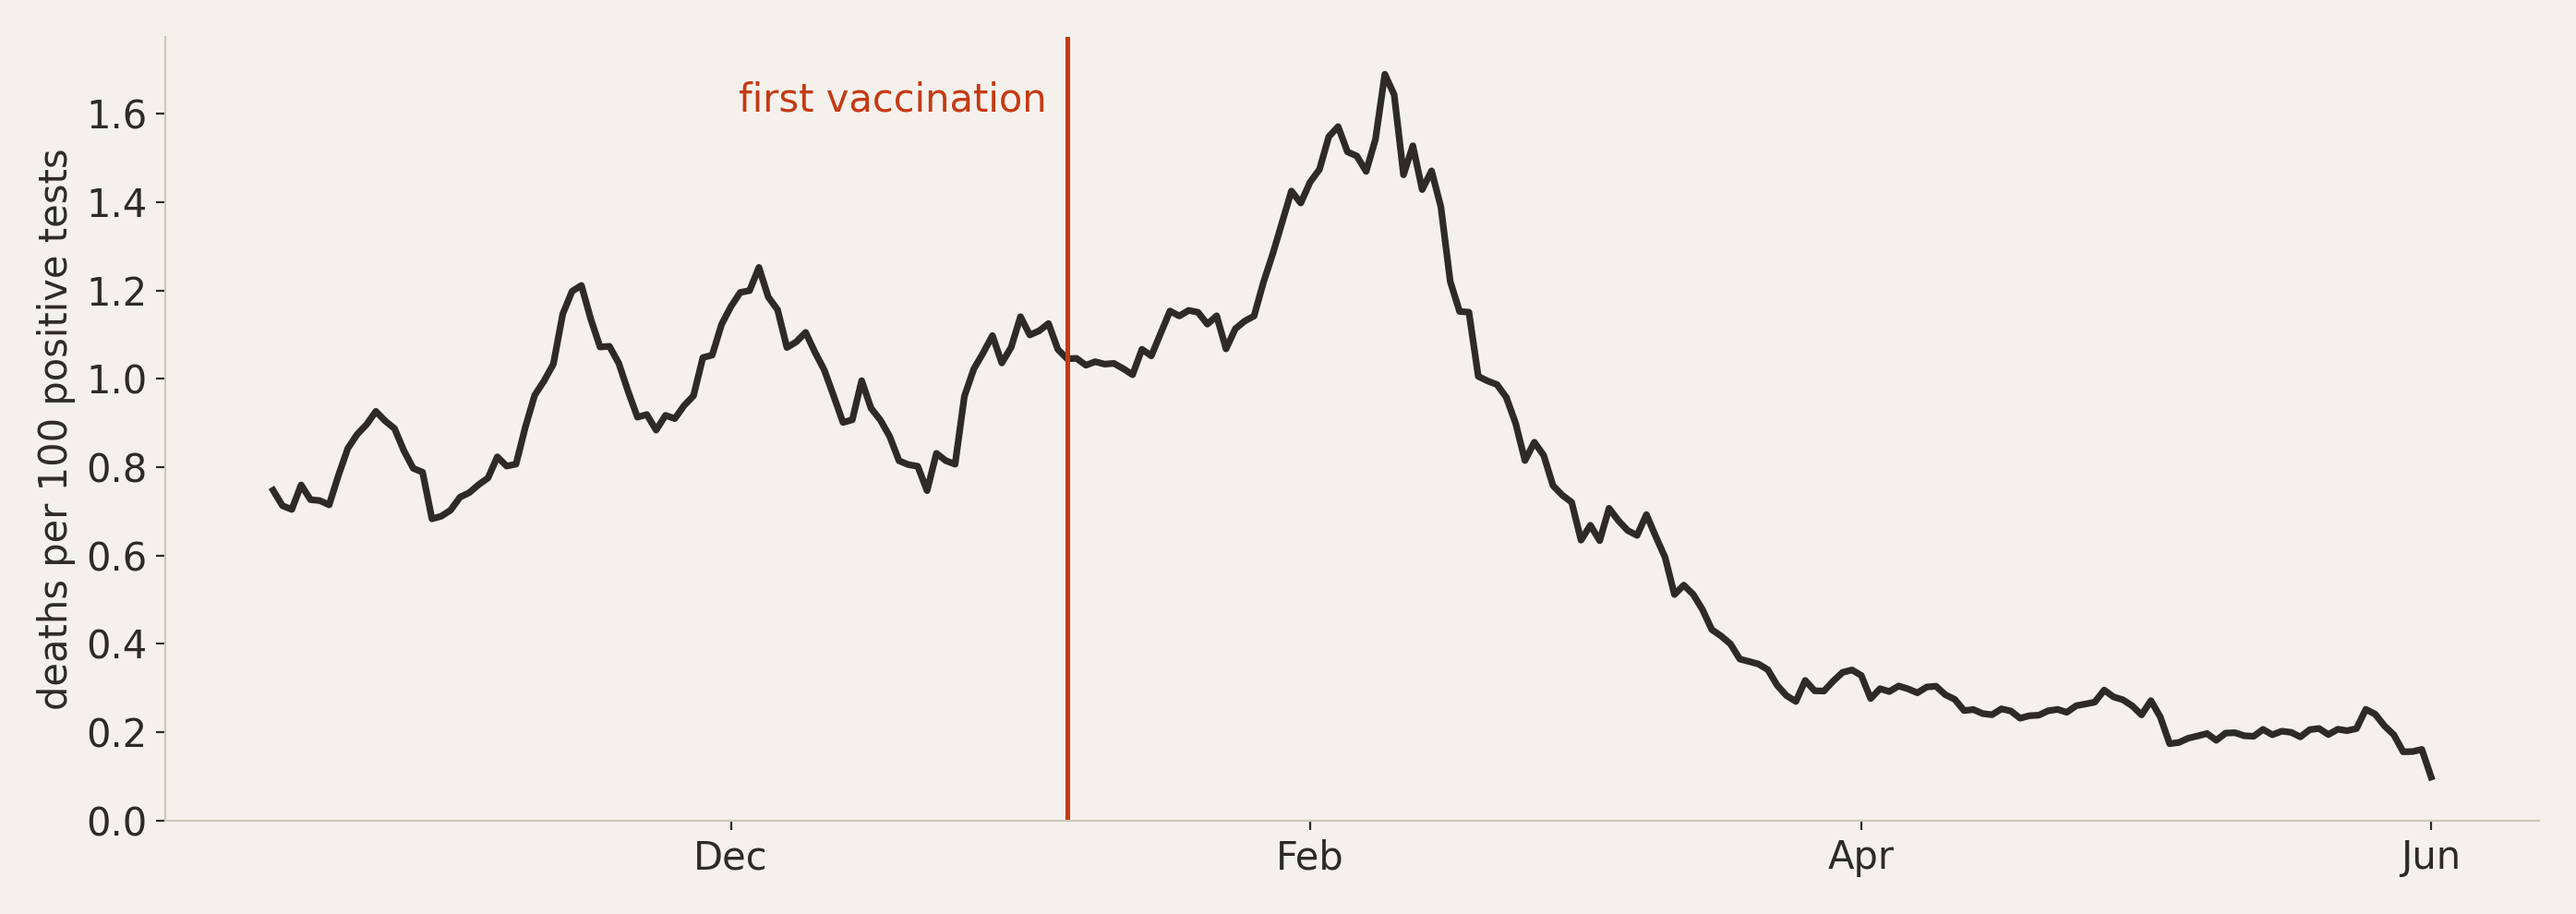
\includegraphics[width=\textwidth]{lesson5/covid_ratio.png}
\caption{Deaths two weeks later per 100 positive tests.}
\label{fig:covid-ratio}
\end{figure}

Through the winter about one death per hundred positive tests, between $0.8$ and $1$, with a bump in early February. Then it falls steeply, to $0.3$ in April and $0.2$ in May. A vaccine doesn't work on one day. The Dutch rollout started on 6 January with care-home residents and the people caring for them, and worked down the age groups from the oldest, through February and March. Slowly at first, then everybody wanted their turn, and at the end a long tail of people who came late or hesitated. Once the most vulnerable groups are protected, the ratio settles lower.

One level, a turn over some weeks, a lower level. Which of the four shapes is that? A logistic, turned downward. Why would the model for duckweed on a pond fit vaccination? Because both grow until they run into a limit: the pond is full, or the vulnerable people have had their turn.

\subsubsection{A logistic switch has two knobs: when and how fast}
The vaccine gets a term of its own, a \emph{switch} $s(t)$:
$$\text{deaths}(t) = a \cdot \text{tests}(t - 14) \cdot s(t) + b + \varepsilon, \qquad s(t) = \frac{1}{1 + e^{-k (t - x_0)}}.$$
Turned downward, the switch starts at $1$: of every positive test, the old share ends in death. Multiplying by one does nothing, so before vaccination this is the same model as before. It ends at $0$: a positive test no longer leads to death. Halfway, at $0.5$, half of the deaths the tests would predict happen.

\begin{figure}[H]
\centering
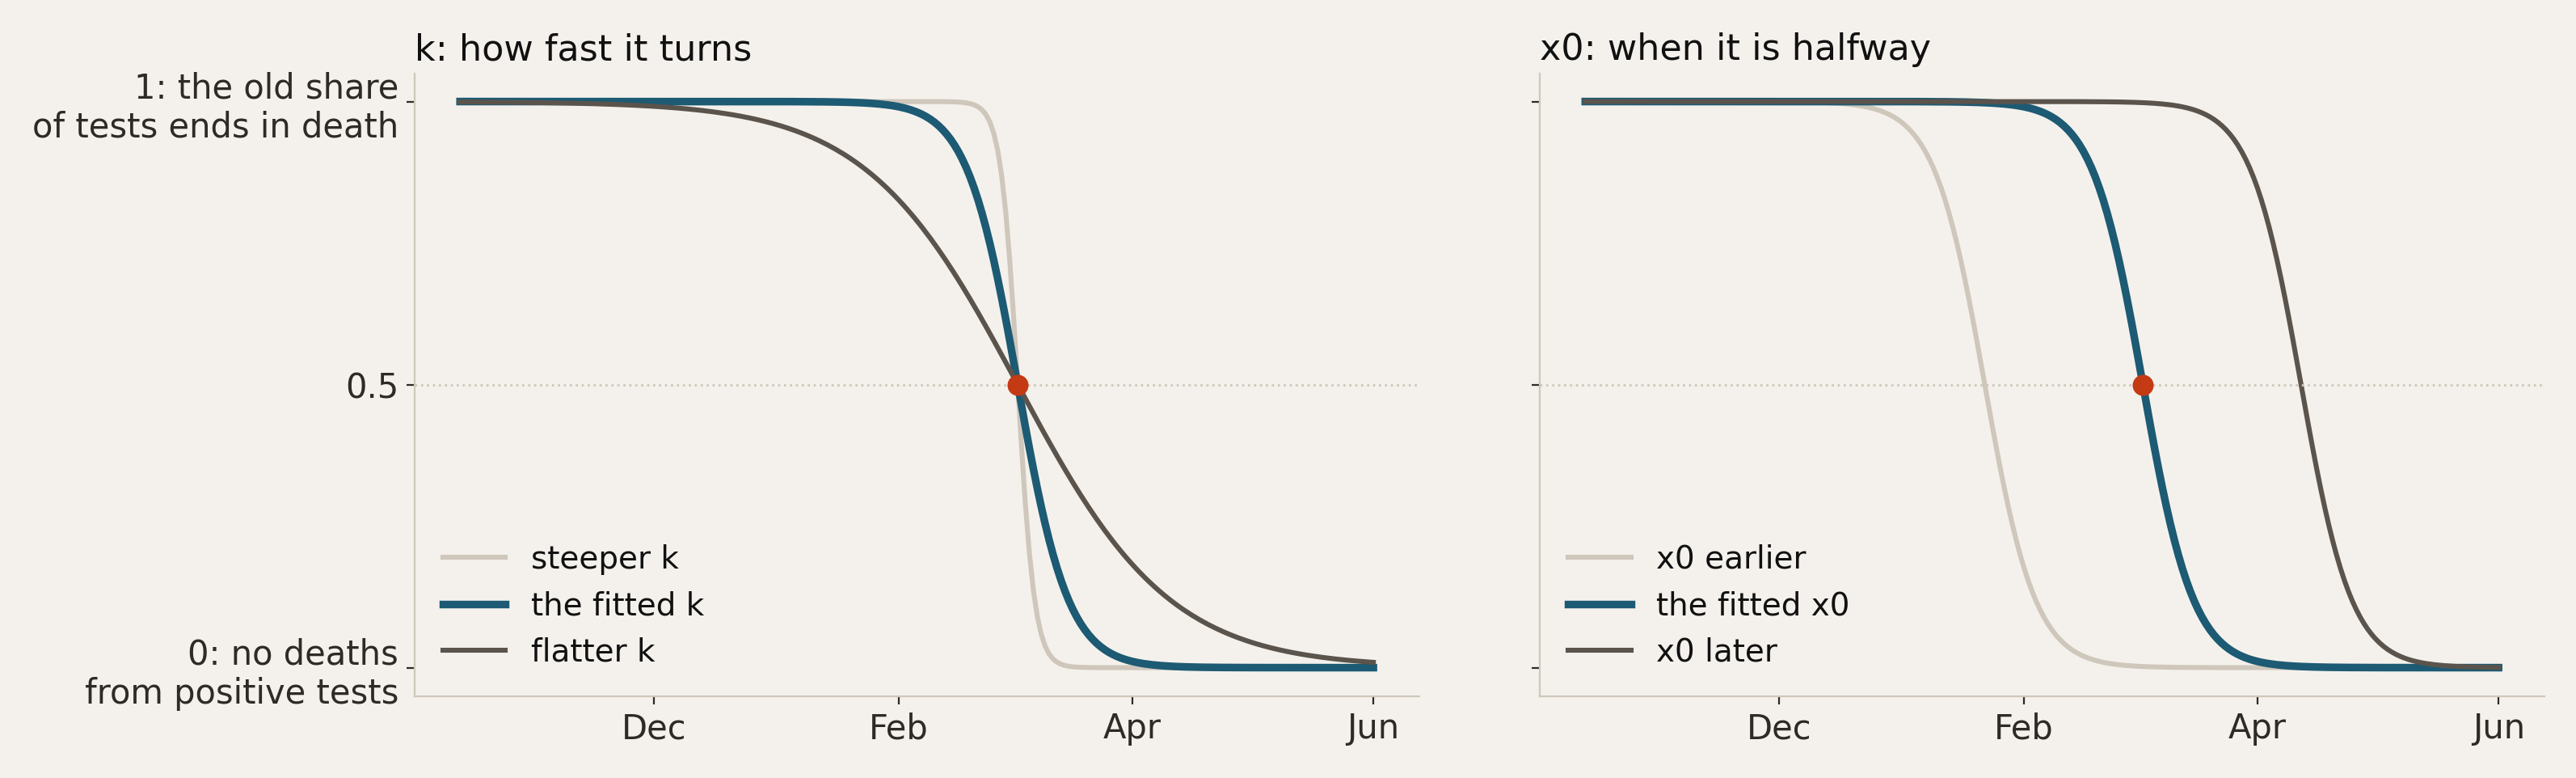
\includegraphics[width=\textwidth]{lesson5/switch_knobs.png}
\caption{Left: the same $x_0$ with a steeper and a flatter $k$. Right: the same $k$ with $x_0$ earlier and later.}
\label{fig:switch-knobs}
\end{figure}

The switch has two knobs. $x_0$ sets \emph{when}: the day the switch is halfway; it slides the curve left and right. $k$ sets \emph{how fast}: a large $k$ turns in days, a small $k$ over months. We don't know either of them, and that is exactly what we want the fit to tell us: here is the formula, here is the data, find out how steep the turn is and where it lies.

Notice where the switch sits. It multiplies only the tests term. When it reaches $0$, what remains is $b$ and the noise: deaths that have nothing to do with positive tests. That is the claim of the model: vaccination breaks the link between testing positive and dying; it does not make other deaths disappear. That is not exactly how the disease works, of course. Even vaccinated people sometimes die of COVID, so you could argue the switch should not go all the way to zero. You can keep refining; at some point that is a job at the RIVM, the Dutch public health institute.

\subsubsection{The switch, fitted: the date falls out of the fit}
Four numbers, fitted together: $a$ and $b$ from the line, $k$ and $x_0$ from the switch. The only help the optimiser got was a starting value for $x_0$, about a month after the first vaccination, and bounds that say what each parameter may mean.

\begin{figure}[H]
\centering
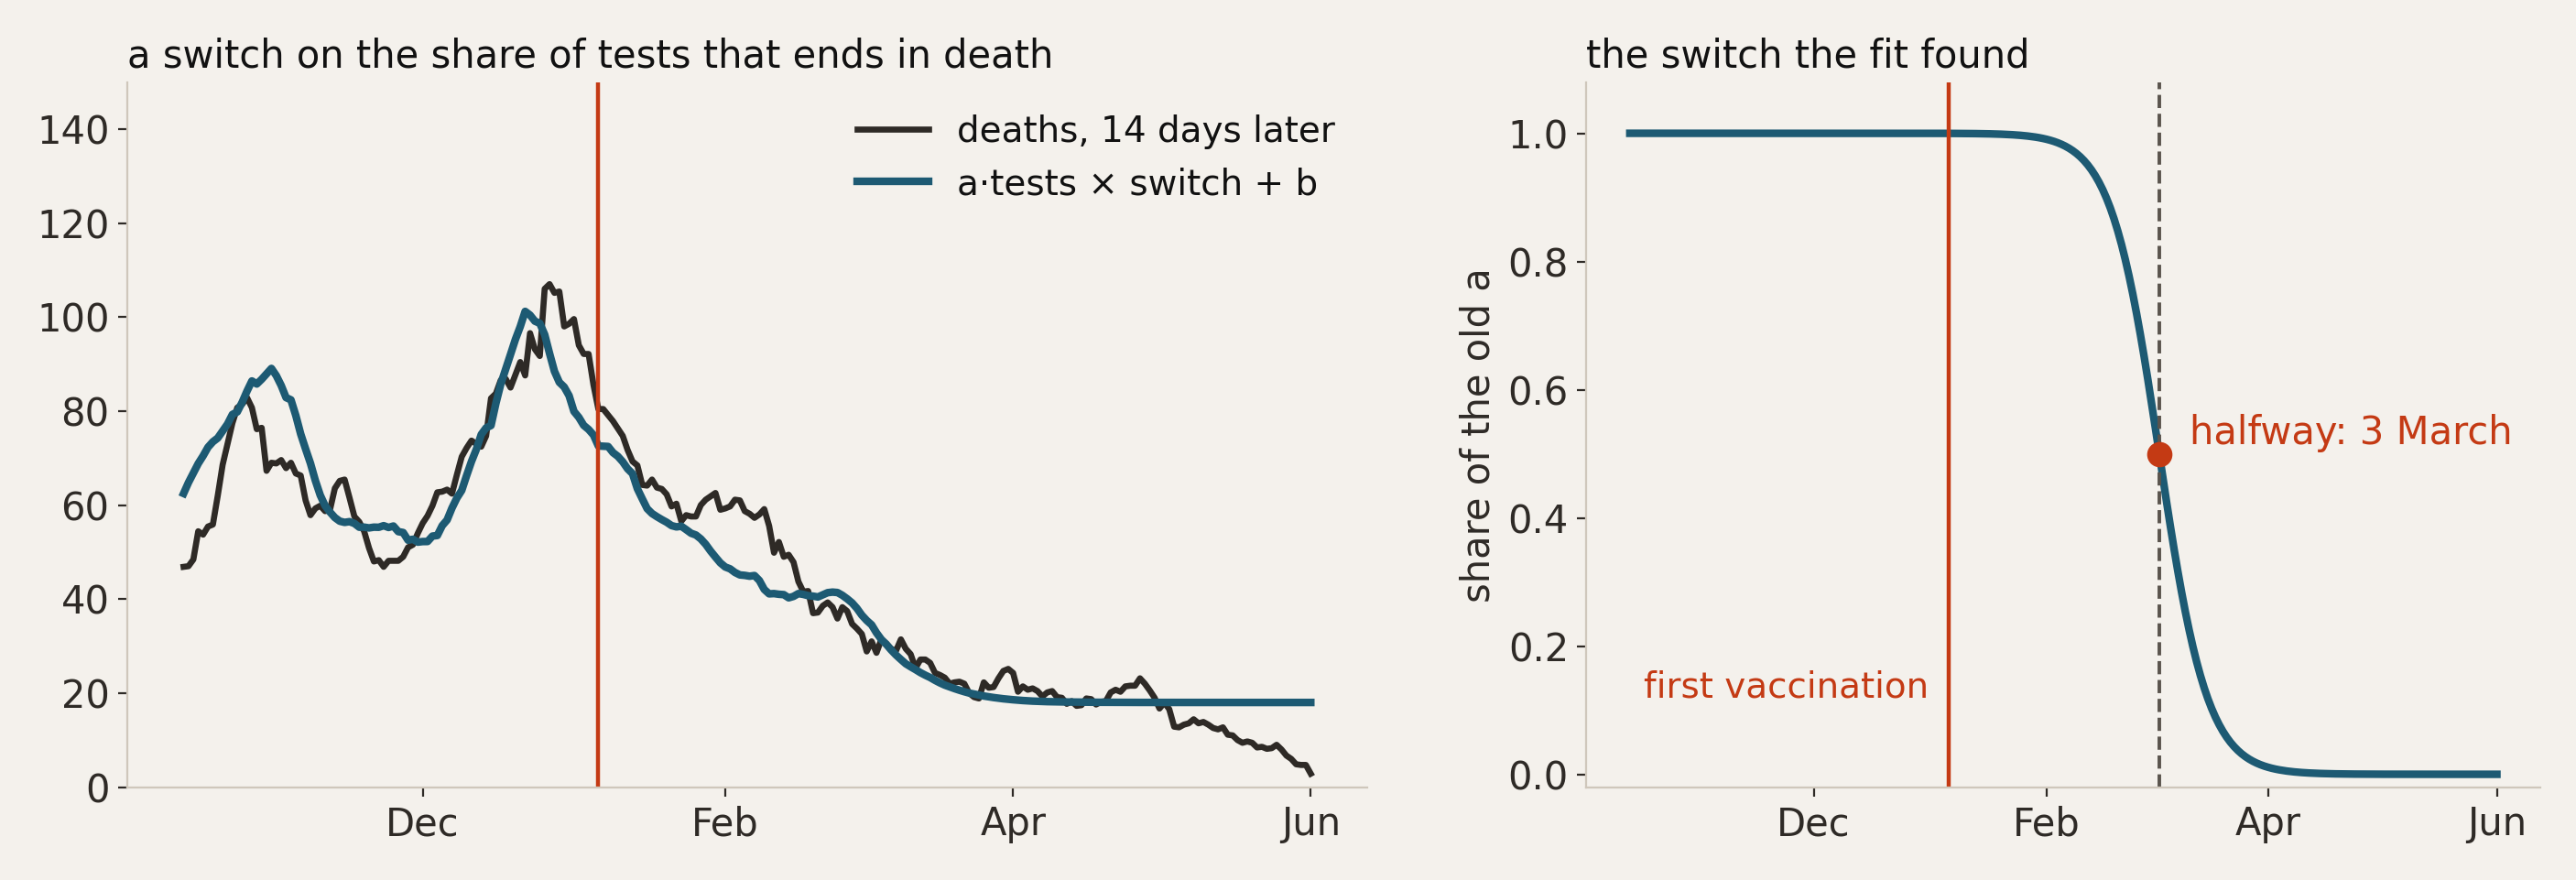
\includegraphics[width=\textwidth]{lesson5/covid_switch.png}
\caption{The model with the switch, over all 232 days.}
\label{fig:covid-switch}
\end{figure}

The fit puts the turn halfway on 3 March 2021, eight weeks after the first vaccination. The turn is fairly quick: the switch is still at $0.99$ on 1 February, $0.58$ on 1 March, and close to $0$ by 1 April. And $a = 0.0071$ and $b = 18$, close to the line fitted before vaccination ($0.0065$ and $20$): the switch doesn't have to bend the line, it only takes the tests term away. The mean squared error drops from $800$ for the line alone to $66$.

Look at what we combined. A time series, with a factor that changes over time. A linear relation between two variables. Something like categories: people who die after a positive test, and people who die anyway. Noise from lesson 4. And a logistic from this lesson. This is not deep learning. It is every lesson so far in one formula, with four numbers you can say out loud.

\subsubsection{The residual looks like chance again}
Is the model done? Apply the bar from lesson 4: no long structure over time, and a distribution the data cannot pin down.

\begin{figure}[H]
\centering
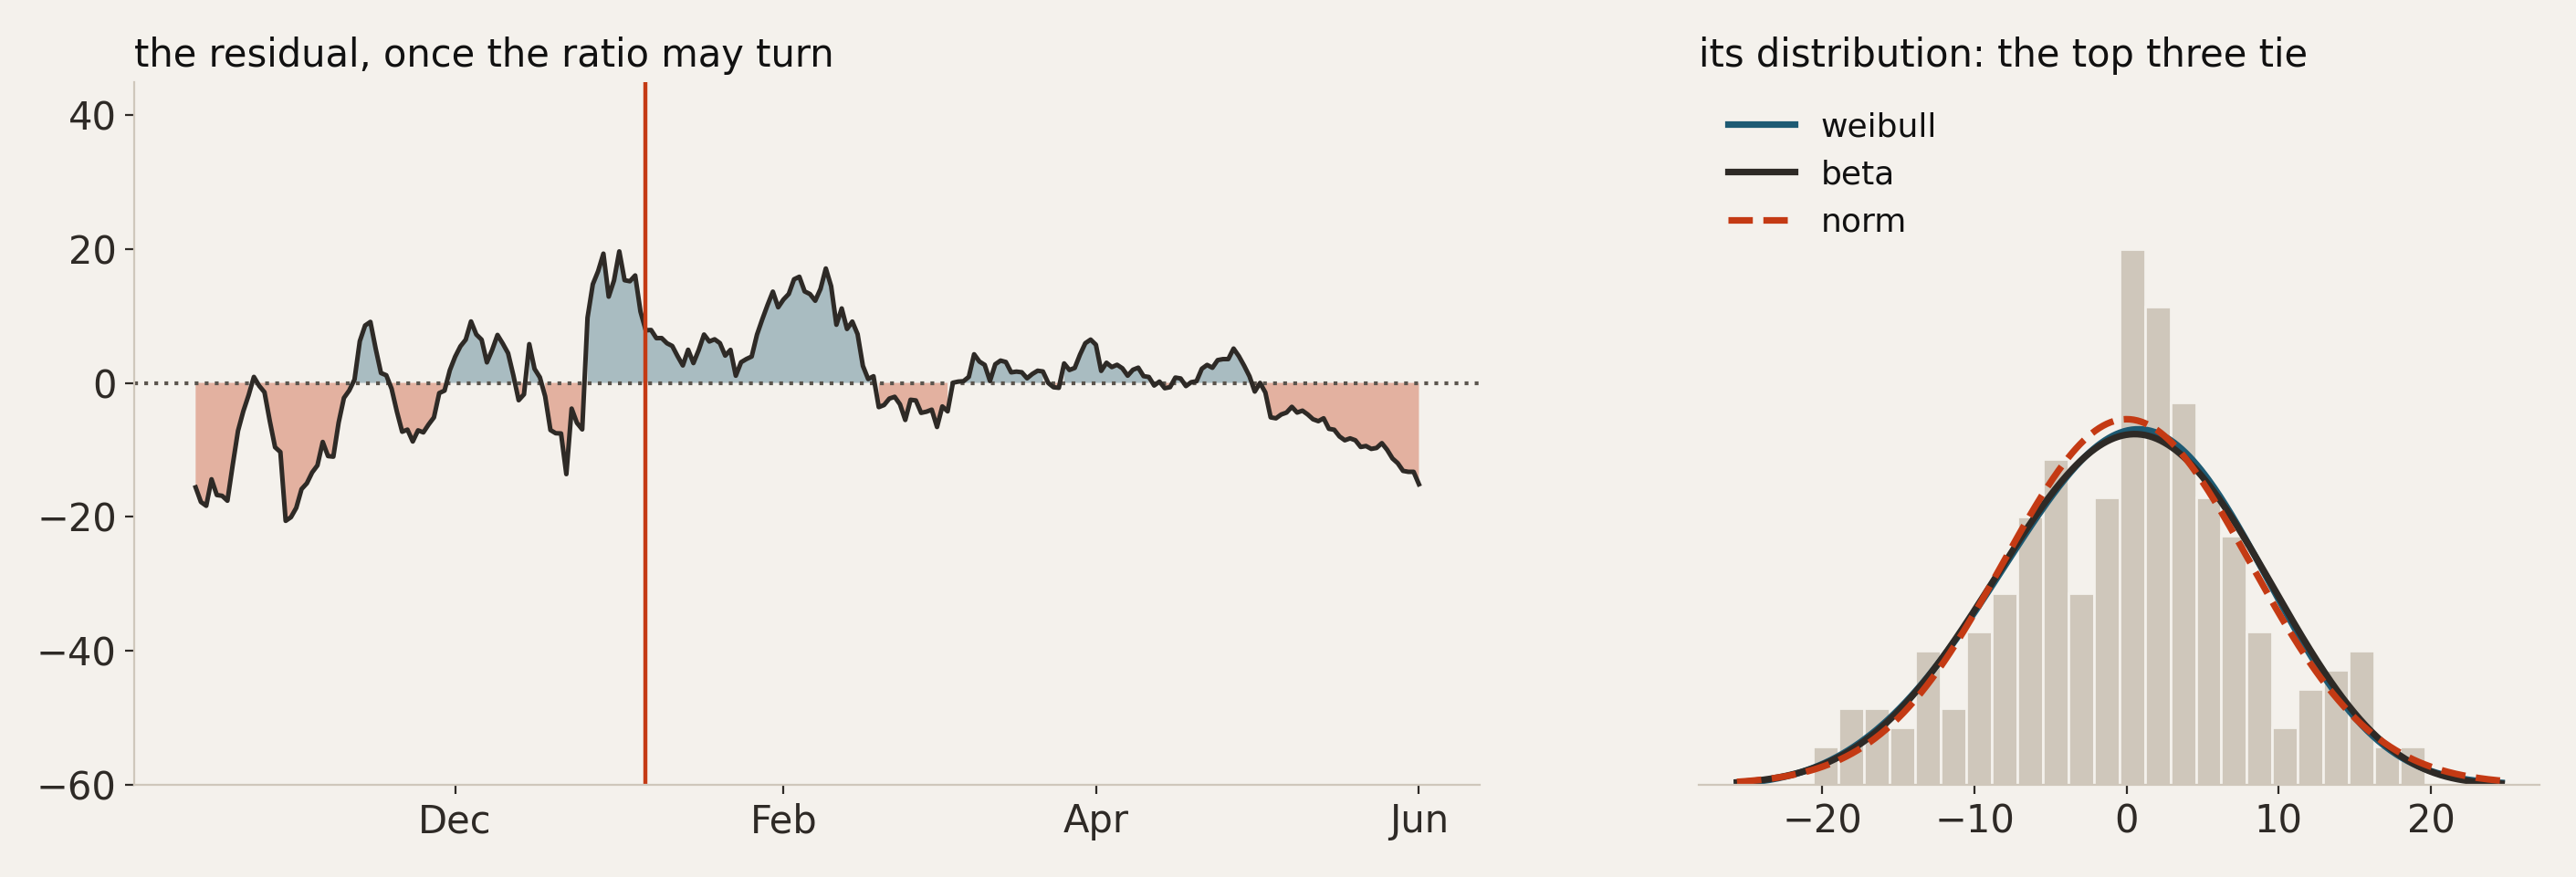
\includegraphics[width=\textwidth]{lesson5/covid_after.png}
\caption{Left: the residual of the model with the switch. Right: its distribution, with the three best families.}
\label{fig:covid-after}
\end{figure}

The long negative run after vaccination is gone; what is left are waves of a few weeks around zero, probably lockdowns and holidays. Weibull, beta and normal fit the errors almost equally well, within about one log-likelihood point of each other, and none is rejected by the KS test. The data can't tell them apart: that is what chance looks like. From May the residual drifts below zero again: the model now says there are $b = 18$ deaths a day, and fewer happen. That is the next thing a serious model would treat. How could $b$ be better modelled, if you think of the four shapes? Perhaps as a season: more people die of flu in December than in June (although in June some die of heat).

Then the honest part. The model has a switch on the calendar, not a term for vaccination. The end of the winter wave, a change in who was being tested (at some point people stopped getting tested) and the order in which age groups were vaccinated all sit on the same calendar, and each could produce a switch that fits. The fit shows that the ratio turned, and when. Why it turned is a separate claim. Defending it needs other evidence: vaccination coverage by age group against deaths by age group, or the same fit on a country whose rollout started on a different date. That would also average out the effect of the Dutch lockdowns. And this happened once: there is no second pandemic to test the model on.

\paragraph{When do you stop?}
That depends on your goal. In lesson 4 we saw that a mechanism that is right $51\%$ of the time on a fifty-fifty bet can make you rich. If you predict whether someone is ill and send them home, a wrong prediction can cost a life, and you need a very different standard. That is why a hospital asks your date of birth eight times before an operation: a very simple test, repeated until it is almost impossible to cut into the wrong patient. Predicting the future is a profession of its own, and a well-paid one. During the pandemic the RIVM ran large Bayesian models with assumptions about everything: what share of people keep a distance, how honest they are when asked, how many keep to the rules at Christmas. At some point the uncertainties multiplied so much that they said they could not predict more than two weeks ahead. That is what honest modelling looks like: you are better than guessing, and you say what you don't know.

I don't expect your own model to become this elaborate. What I wanted to show is the process: you take a step, something is left over, you investigate it, you model it, and something is left over again. And then you stop when what is left looks like real noise.

\subsubsection{The whole loop as a map, drawn by atlas}
The loop we just built also lives in \texttt{scripts/covid\_pipeline.py}: six small functions and a \texttt{main} that runs them in order.

\begin{verbatim}
def main() -> None:
    data = preprocess()
    plot_zscores(data)
    data = fit_model(data)
    plot_model(data)
    plot_residual(data)
    plot_residual_distribution(data)
    logger.success("All done.")
\end{verbatim}

Atlas, a tool I wrote for this course\footnote{\url{https://github.com/raoulg/atlas}, with an install script for macOS, Linux and Windows.}, draws what that code does (figure~\ref{fig:atlas}). It doesn't show files and folders; it shows where data rests and the functions that carry it from one place to the next, in the order they run. Read it from left to right: the command starts the script, \texttt{preprocess} makes a DataFrame (the goad pipeline from table~\ref{tab:covid-pipeline}), \texttt{fit\_model} turns it into a second DataFrame with the prediction and the residual, and the plotting functions write PNG files. A rounded pill is a function, a box is where data rests: a DataFrame in memory, a file on disk. Click a pill and atlas opens it into its own steps.

\begin{figure}[H]
\centering
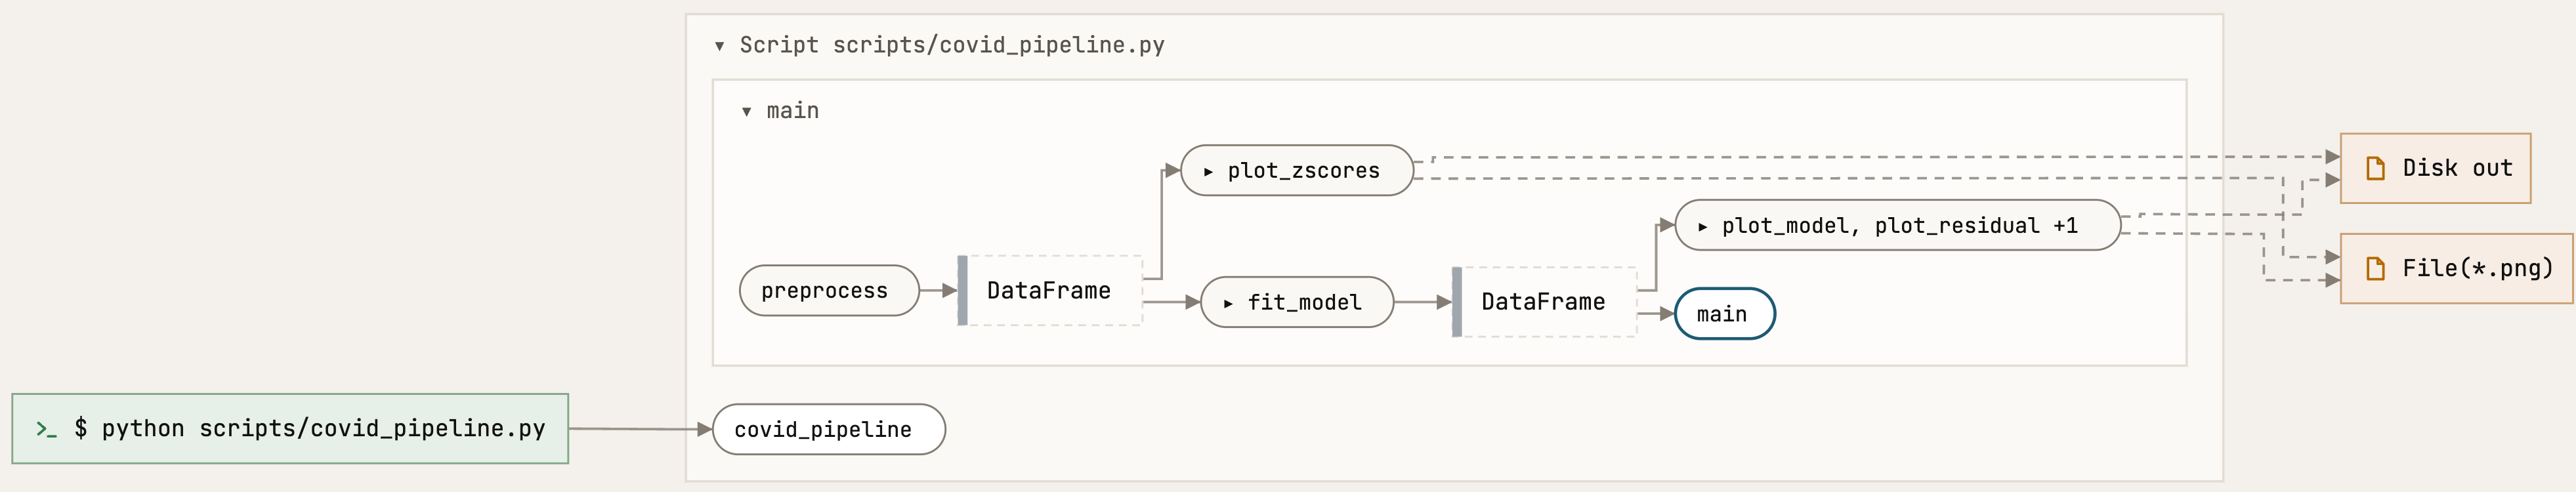
\includegraphics[width=\textwidth]{lesson5/atlas_route.png}
\caption{\texttt{scripts/covid\_pipeline.py}, drawn by atlas.}
\label{fig:atlas}
\end{figure}

The idea behind atlas is that consistent, logical code gives a consistent, simple picture. The same plot can be produced by tidy code and by messy code, and the pictures will look very different: global DataFrames that get written and read somewhere along the way, steps whose order you can no longer see. A linter doesn't notice that: if you make three plots that are really one flow, only you know it should look like one flow. When the picture looks wrong, the code usually is, and the red marks show where atlas misses information: unclear inputs, unclear outputs. It works the same for Python and Rust, and you can give the picture to Claude to discuss what to change. In the final assignment you use it to show how your own code works: run \texttt{atlas view} in your repository, pick your entry point, and be ready to explain the picture. Section~\ref{sec:atlas} says why a picture of your code helps, and how to read one.

\againconcretely
One line, then one switch. The line from before vaccination kept its two numbers; the switch added two more and found the turn eight weeks after the first vaccination, without being told. Look, think, add one step or one term, then read the residual. Each piece of reasoning has a place: the pipeline, or the formula. Stop when what is left looks like chance, and say what the model cannot tell you: here, why the ratio turned.

% ─────────────────────────────────────────────
\subsection{When should you believe a pattern?}
\label{sec:believe}
In lesson 4 you shuffled labels to see how big a difference chance makes for one comparison. Now: what happens when you make many comparisons, and what makes a finding believable at all? The data is the Ubuntu IRC chat channel you know from earlier lessons.

\subsubsection{Fifteen comparisons, one below the line}
Everyone in \#ubuntu-uk with at least thirty messages, $442$ people, and fifteen numbers per person: message length, links, questions, posting at night, and so on. Each person also has a cohort label, A or B. Test every number between the cohorts with a t-test, and put the fifteen p-values on a log axis with the usual line at $0.05$.

\begin{figure}[H]
\centering
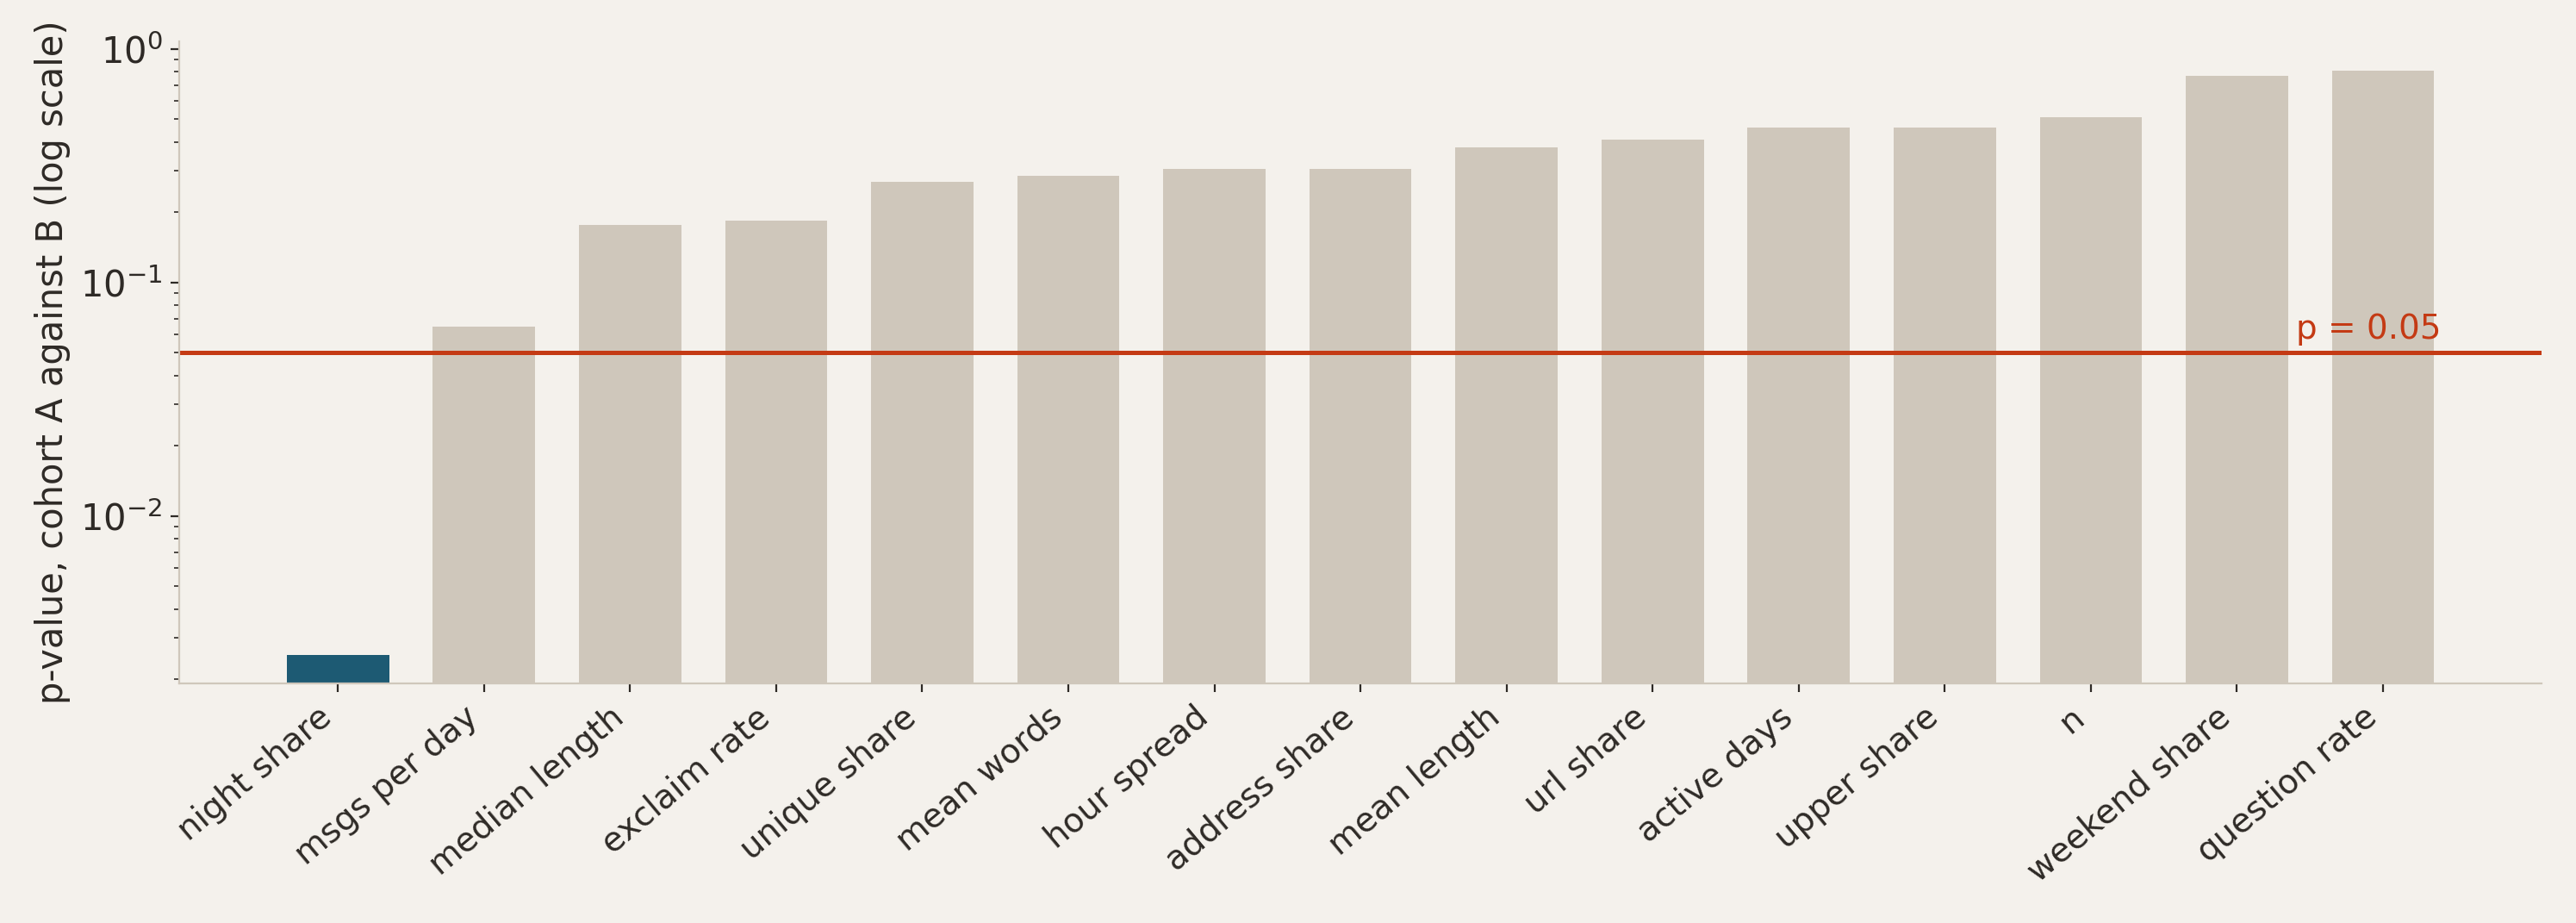
\includegraphics[width=\textwidth]{lesson5/hunt.png}
\caption{Fifteen measures, cohort A against cohort B. The dashed line is $p = 0.05$.}
\label{fig:hunt}
\end{figure}

One clears the line easily: cohort A does $13.5\%$ of its posting between midnight and five in the morning, cohort B $6.7\%$, $p = 0.003$, with more than two hundred people per group. That sounds publishable, and a story arrives at once: night owls, or another time zone. Notice how fast the story came. Now look at how the cohorts were made: with a random permutation. The two groups are the same population, split at random. There is no cohort. Everything in this plot was produced by nothing at all.

\subsubsection{How often do you find something when there is nothing?}
So measure it instead of being surprised. Shuffle the cohort labels $300$ times and hunt every time over the fifteen measures.

\begin{figure}[H]
\centering
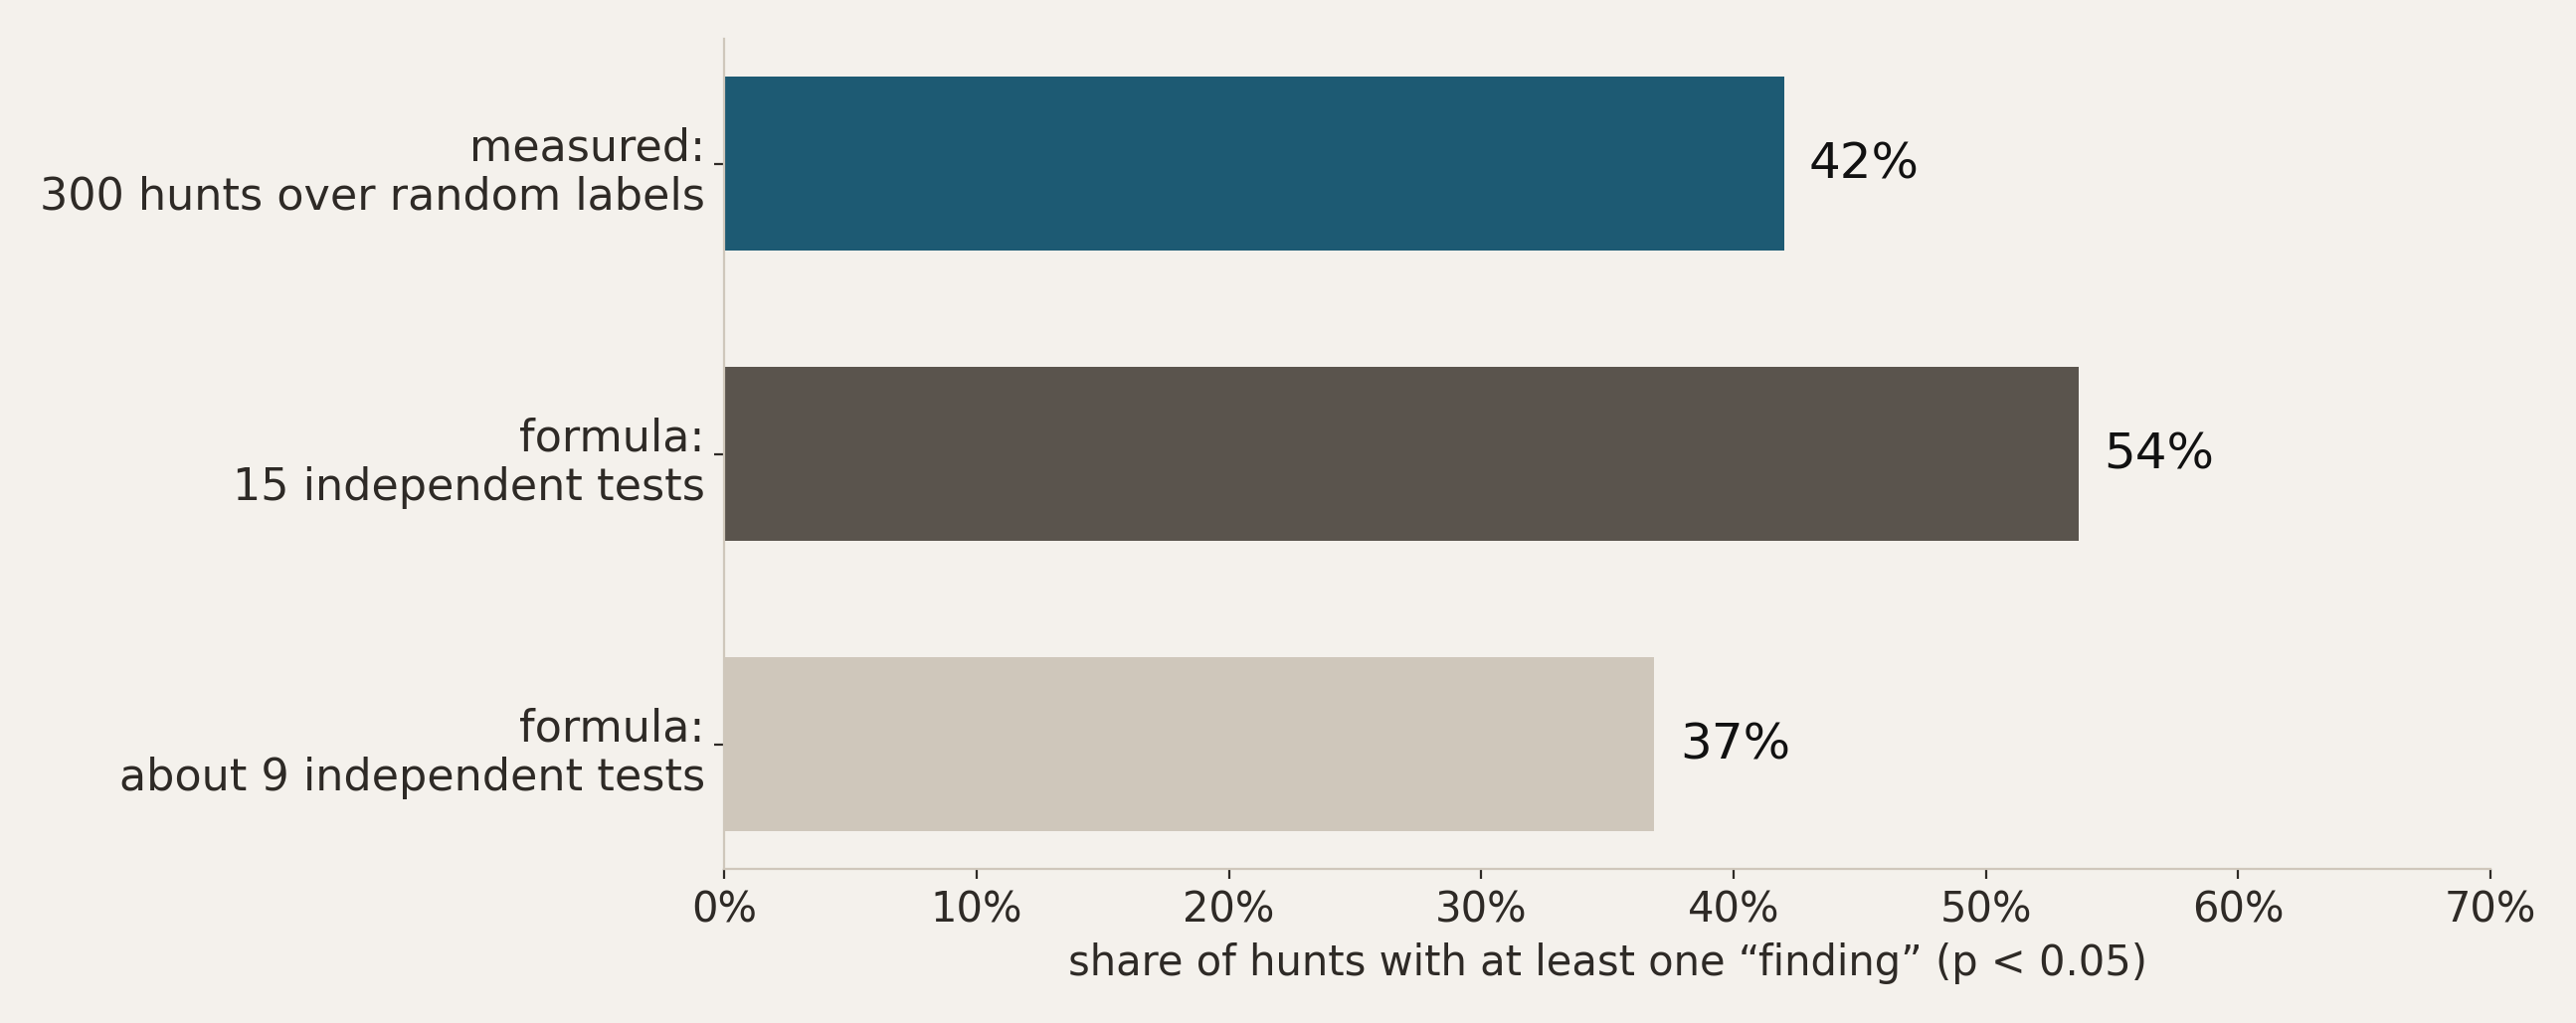
\includegraphics[width=\textwidth]{lesson5/null_hunts.png}
\caption{300 hunts over random labels: how many of the fifteen measures cross $0.05$.}
\label{fig:null-hunts}
\end{figure}

In $42\%$ of the hunts at least one measure crosses $0.05$; some find two or three. That is the baseline: before asking whether a finding is real, ask how often you would find something if there were nothing to find. If the answer is almost half the time, finding something is not evidence.

The arithmetic is worth knowing. A p-value below $0.05$ means a false alarm one time in twenty per test. ``At least one alarm'' is hard to count; ``no alarm at all'' is one product. Fifteen independent tests all stay quiet
$$0.95^{15} = 0.46$$
of the time, so at least one alarm $54\%$. The measured $42\%$ is lower because the measures overlap: mean length, median length and mean number of words are three names for message size. The fifteen behave like about nine independent measures, and $1 - 0.95^{9} = 0.37$.

This is the dice from lesson 4 again. If I say beforehand that you will roll six sixes and you do, that means something. If I let a hundred thousand people roll and one of them rolls six sixes, I should expect it. With few messages and few people, as in your own chats, the chance of a lucky find is large. Ask beforehand: how many things am I testing, and what would I find by chance alone?

\subsubsection{A real pattern predicts people it hasn't seen}
The strongest defence is to split the data: find the pattern in one part, then predict the other. Here with fresh random cohorts, so again there is nothing to find.

\begin{figure}[H]
\centering
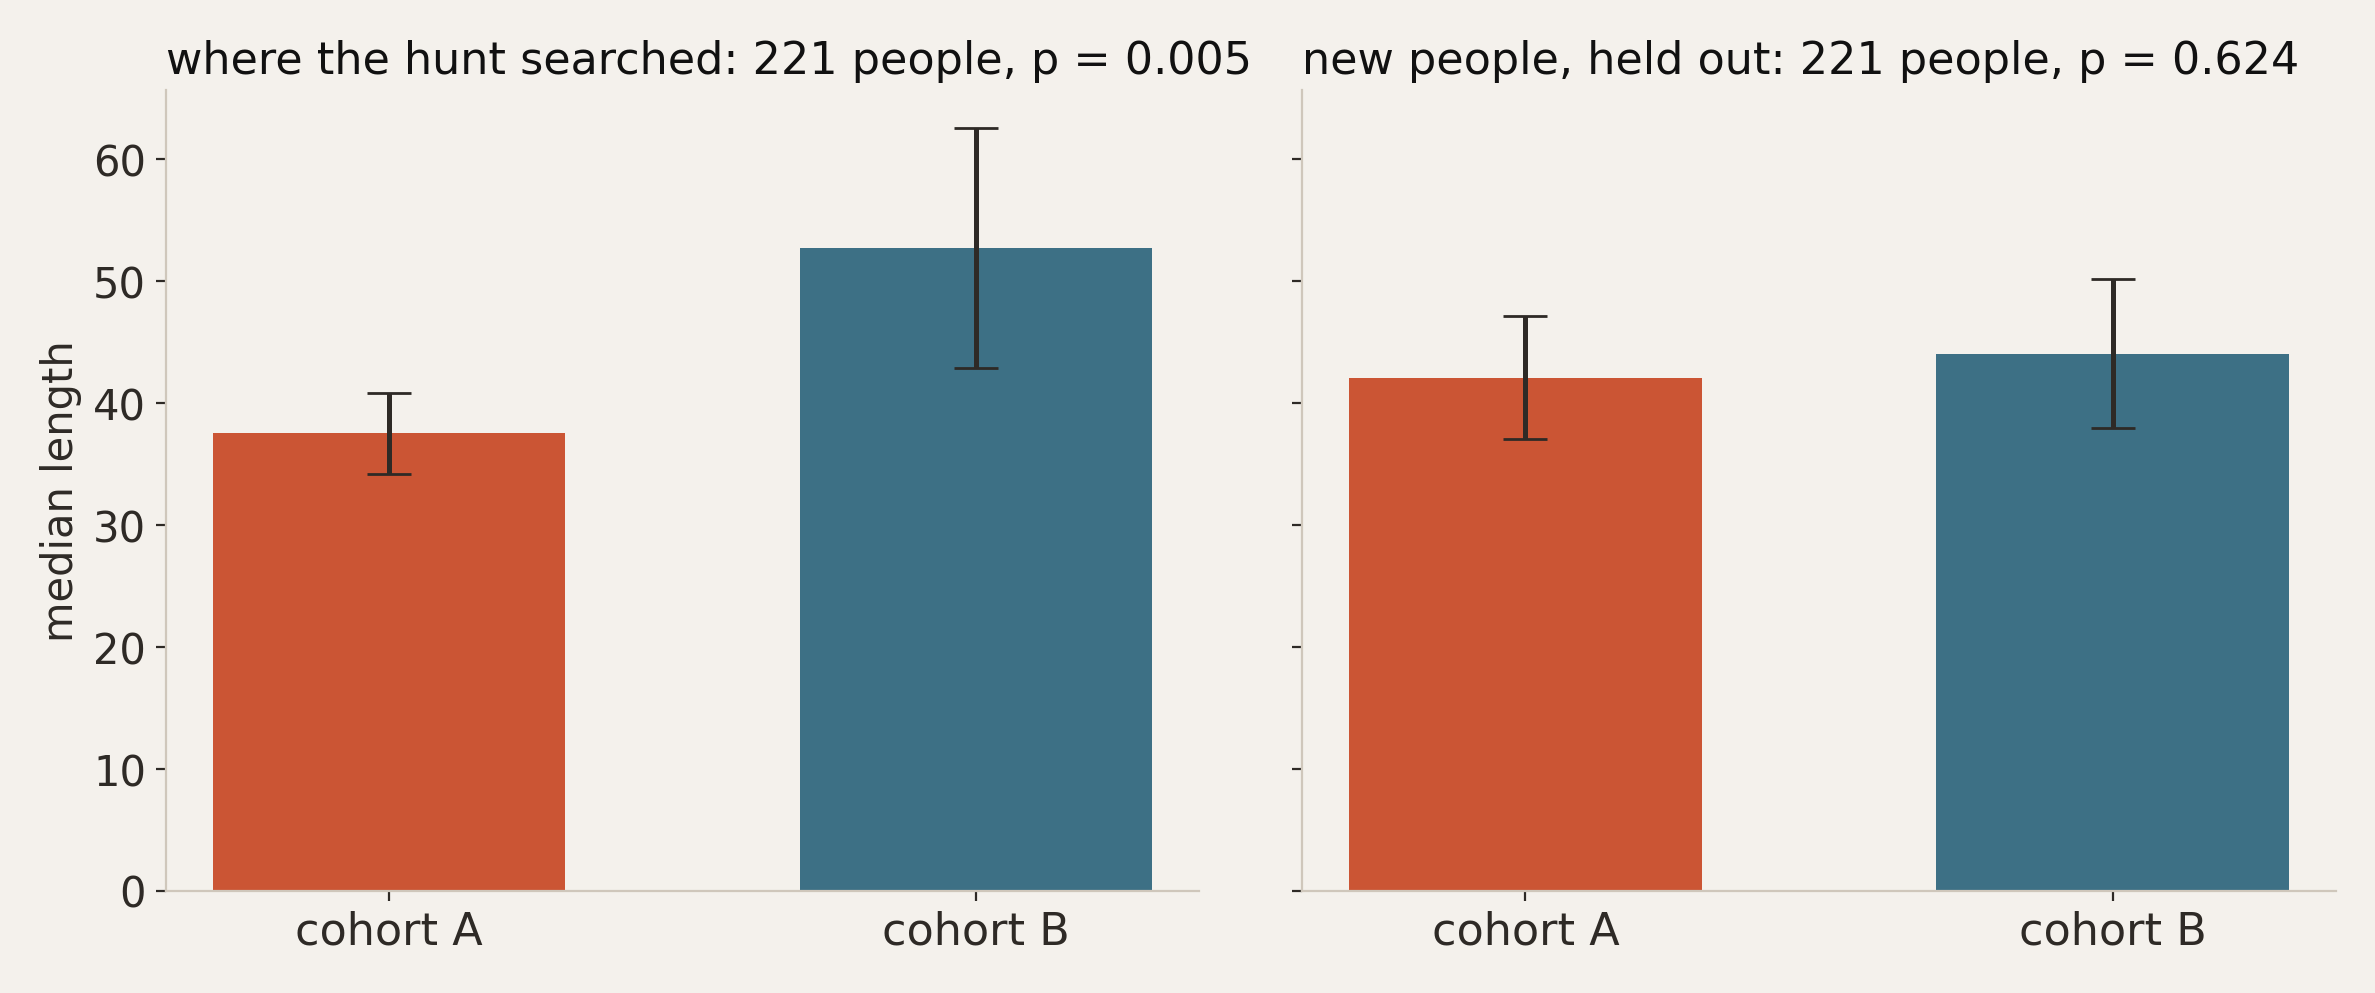
\includegraphics[width=\textwidth]{lesson5/held_out.png}
\caption{Left: the hunt in half of the people. Right: the same comparison in the other half.}
\label{fig:held-out}
\end{figure}

Hunt over the fifteen measures in half of the people: cohort A writes clearly shorter messages, $p = 0.005$, a difference you would happily report. Then look at the other half, people the hunt never touched: the gap is gone, $p = 0.62$. Over $200$ random splits, the hunt in the first half finds something below $0.05$ in $40\%$ of the splits, and the new people confirm it $2\%$ of the time. A real pattern predicts new data; an accident of the search does not. With enough data you can make this a habit: use $80\%$ of your data to search, as freely as you like, knowing that some of what you find is nonsense, and keep $20\%$ apart to see what survives.

One caution: the held-out part has to consist of new units of the claim. Splitting the same people into an early and a late period is not enough, because the same people carry the same accidents into both periods; in this channel such a time split confirmed random cohort differences about one time in five. And a finding belongs with the search that produced it: say how many things you looked at.

\subsubsection{Three legs make a finding believable}
If the hunt were the whole story, the conclusion would be that nothing is ever real, which is as bad as believing everything. So what would make you believe a finding? Three legs, and statistics gives you at most one of them.

\begin{enumerate}
\item \textbf{A model.} A statistical model that fits: enough observations at the level of the claim, an effect bigger than chance. It can be evidence, if used well, but even with $p < 0.05$ it can still be chance.
\item \textbf{A mechanism.} A reason it would be true, that you could have named before looking. No data gives you this.
\item \textbf{Replication.} It shows up where you didn't look: another period, another group, another way of measuring.
\end{enumerate}

\begin{table}[H]
\centering
\begin{tabularx}{\textwidth}{@{}l X X@{}}
\toprule
 & \textbf{Survives testing} & \textbf{Fails testing} \\
\midrule
\textbf{Mechanism} & Report it, then look for replication. & ``Plausible, unproven.'' A finished result: say what would settle it. Or the test was wrong. \\
\textbf{No mechanism} & Don't conclude yet. A fluke, or a variable you haven't named. & Drop it. \\
\bottomrule
\end{tabularx}
\caption{Mechanism against testing.}
\label{tab:legs}
\end{table}

The two cells on the diagonal are obvious. The other two are the lesson. A mechanism that fails testing is a finished result if you say what would settle it, and sometimes it means you tested the wrong way; the next example is one. A significant result without a mechanism is not a conclusion but a question: a fluke, or a confounder you haven't named, and the confounder is usually the more interesting finding. A mechanism also has a risk of its own. A surprising claim, against intuition, gets critical eyes. A claim that confirms what people already thought is accepted too quickly, and then the digging stops. The COVID switch, by the way: a model that fits, a mechanism yes, replication not yet.

\subsubsection{The comparison you choose is part of the claim}
The first claim through the grid: Ubuntu release days are busier. The mechanism is strong. Ubuntu releases on a Thursday, twice a year, on dates fixed in advance by a calendar the chat has no say in, and people in the channel have a reason to show up: have you seen the new version?

\begin{figure}[H]
\centering
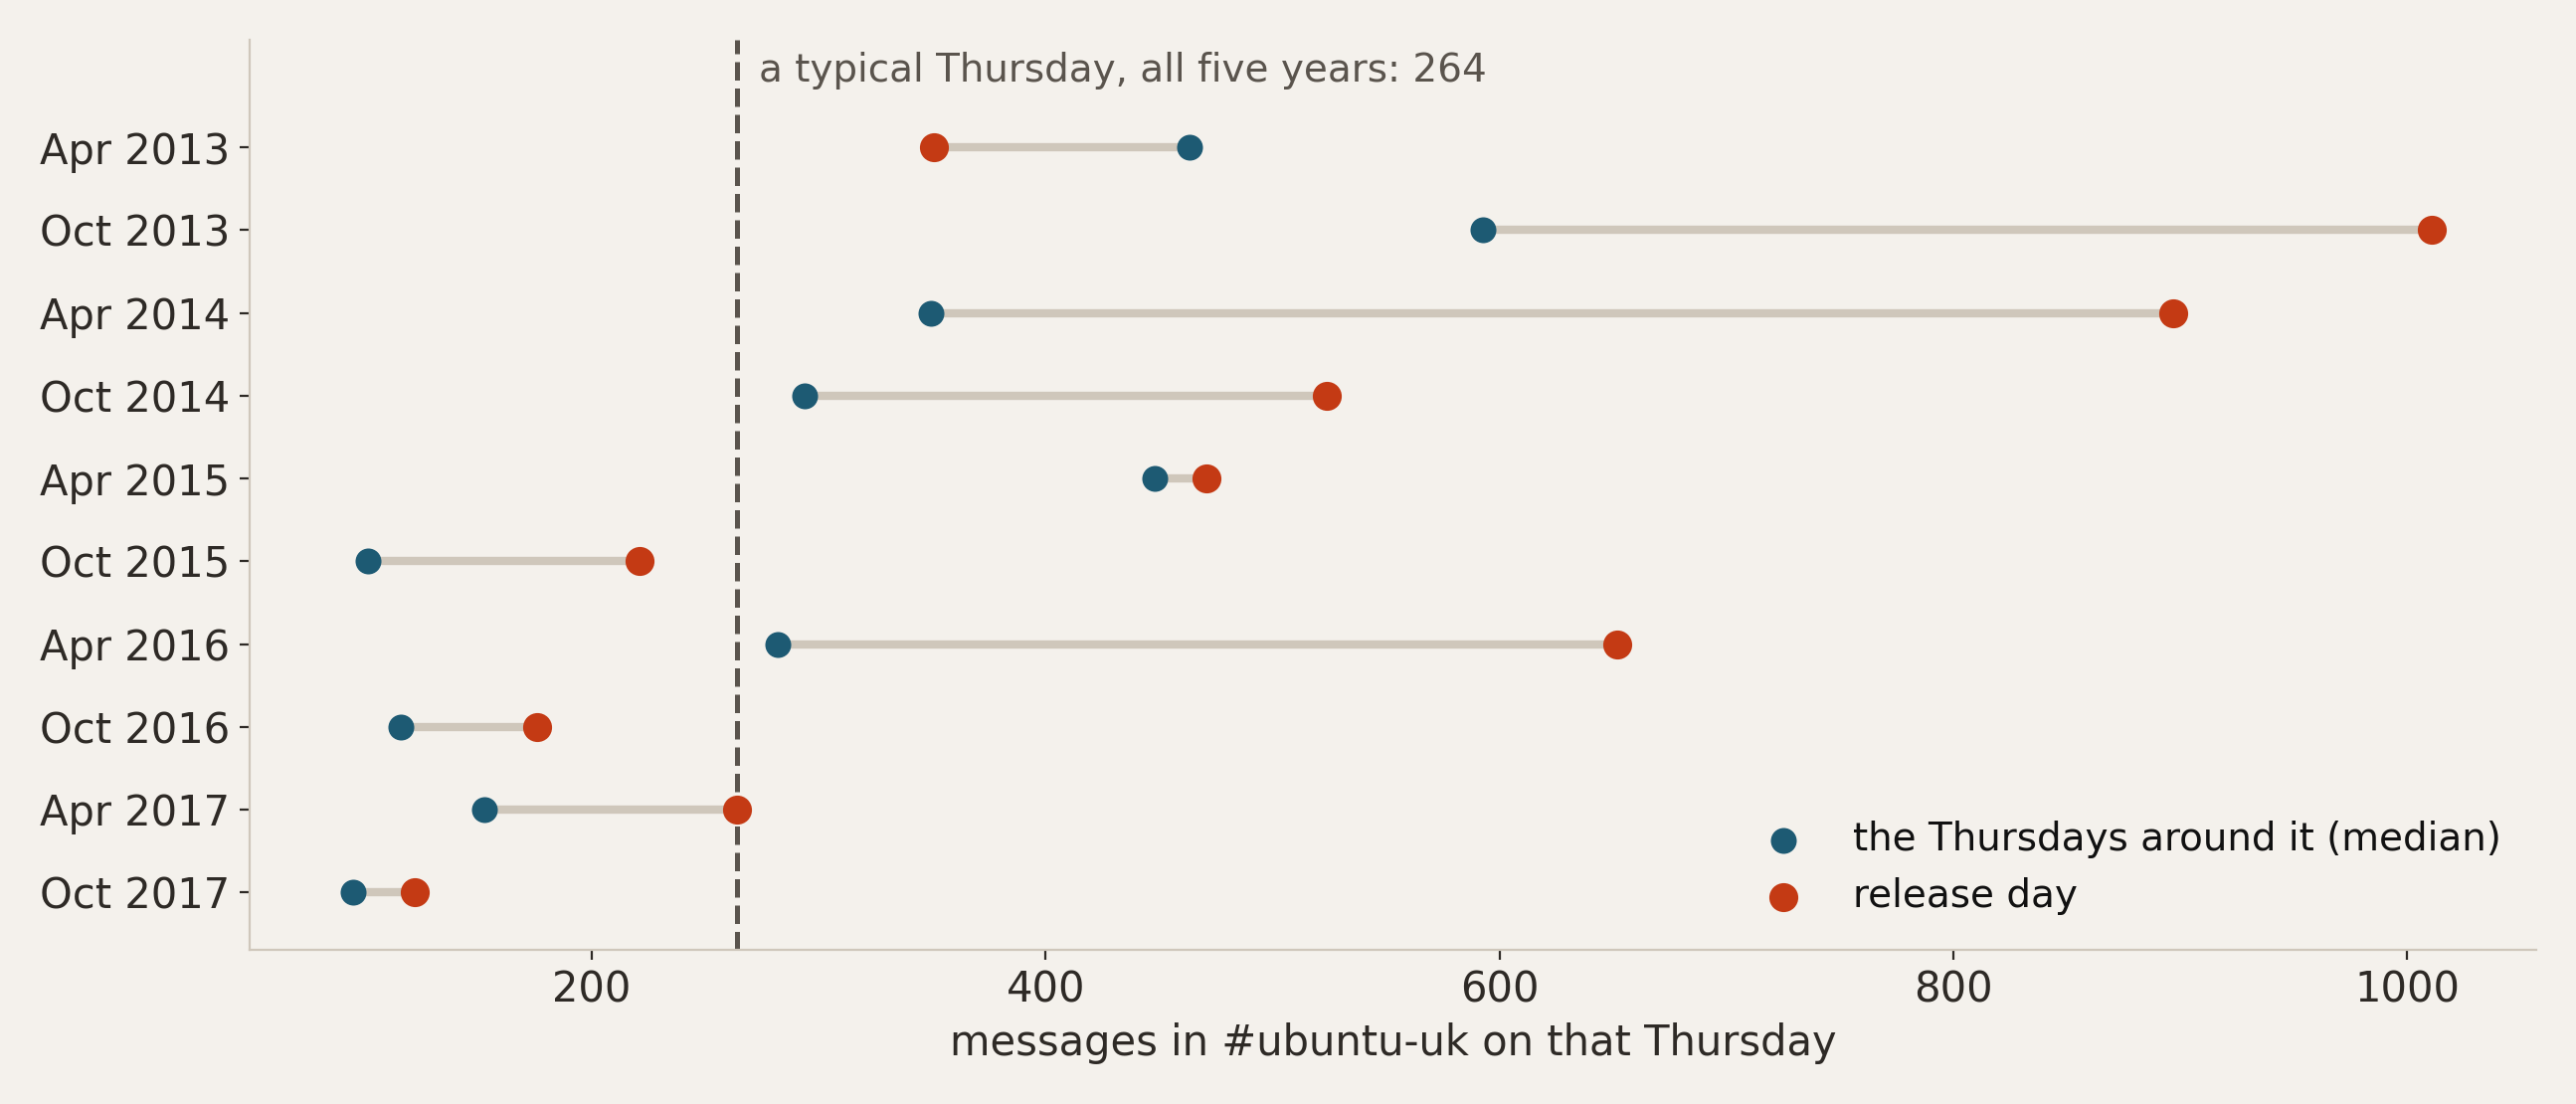
\includegraphics[width=\textwidth]{lesson5/release.png}
\caption{Ten release days against a typical Thursday of all five years (dashed), and against the Thursdays around each release.}
\label{fig:release}
\end{figure}

The obvious test compares each release day with a typical Thursday. Over all five years, the median Thursday has $264$ messages, and only six of the ten releases beat it: a coin flip, which would kill the claim. It shouldn't, because the channel lost most of its traffic over these years. A typical Thursday in 2013 and one in 2017 are different numbers, and the late releases are compared with a median that mostly comes from the busy early years. The trend is a confounder for the event. Compare each release with the Thursdays within four weeks around it instead: nine of ten are busier, by $1.7$ times on average, and a sign test gives $p = 0.02$. The sign test only asks on which side of typical each day falls, a question ten noisy days can answer. Same data; only ``typical'' changed. A correct mechanism can fail on a badly chosen reference.

\subsubsection{Test at the level of your claim}
The claim: people write longer messages in the weekend. Per message, the answer looks decisive: weekend messages are $49.2$ characters on average against $48.2$ on weekdays, with $p = 10^{-9}$ over $510{,}833$ messages.

\begin{figure}[H]
\centering
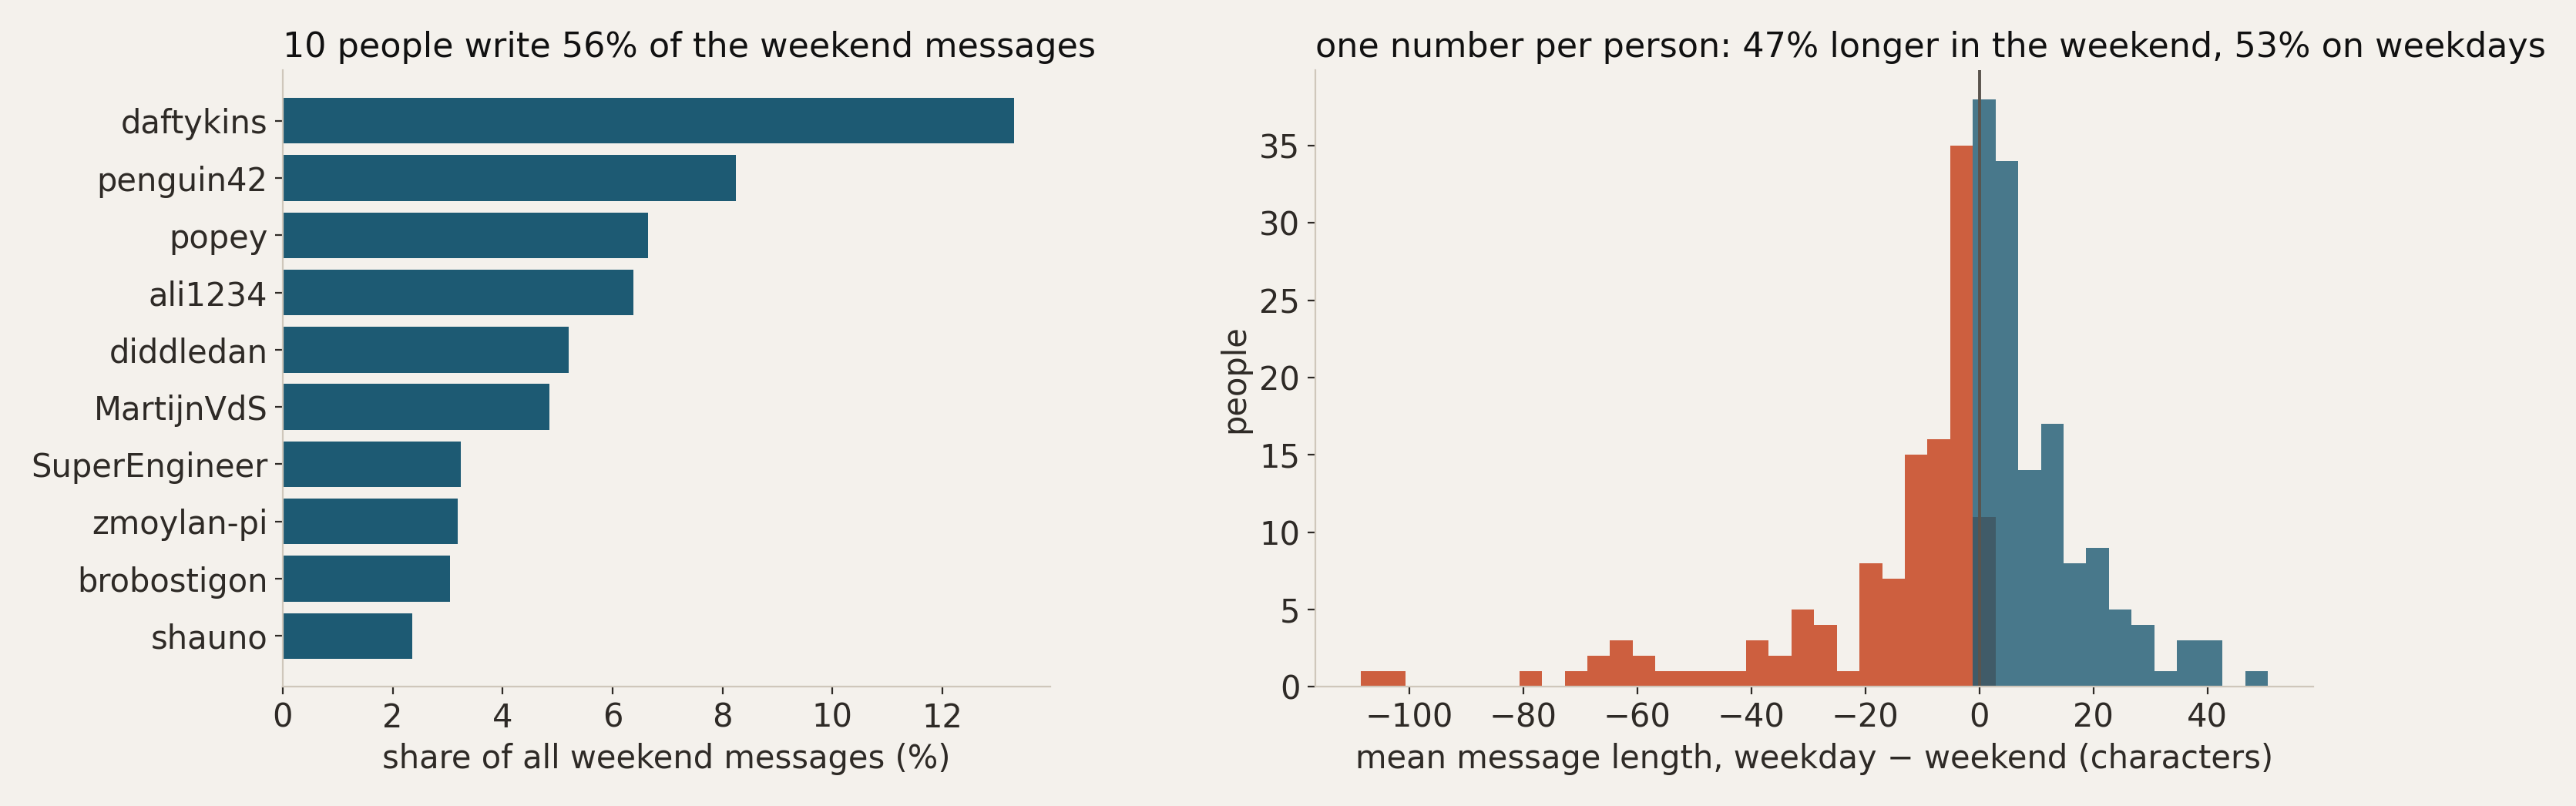
\includegraphics[width=\textwidth]{lesson5/weekday.png}
\caption{Left: ten people write 56\% of the weekend messages. Right: weekday minus weekend message length, one number per person.}
\label{fig:weekday}
\end{figure}

But a message average is dominated by whoever writes the most. Ten people write $56\%$ of all weekend messages, daftykins alone about $13\%$, and who posts in the weekend is not who posts on weekdays. If every weekend poster wrote exactly as they do on weekdays, the weekend average would already be $48.9$ instead of $48.2$: most of the difference is who is talking, not how people talk. Bill Gates walks into a bar, and on average everyone is a millionaire. Nobody in the bar got richer.

Ask the question at the level of the claim, one number per person, and it splits: $47\%$ write longer in the weekend, $53\%$ on weekdays (perhaps during office hours, out of boredom), paired $p = 0.06$. Outside the small group of heavy posters, there is no effect at all. Report it that way: no general difference between weekday and weekend writing for the $259$ people with enough messages; the per-message difference comes from who posts when. Your claim is about a few people, not about half a million messages.

This is the statistician's nightmare: dig deep enough into your data and you can always find a subgroup that makes your effect disappear, or turn around. That is not a reason not to dig. It is a reason to dig: don't stay at the surface, look for the subgroups, and state your claim at the level where it holds.

\againconcretely
Spurious correlations should be expected. With enough features and enough observations, you always find something; the right question is not ``did I find something?'' but ``how often would I think I found something if there were nothing?'' Shuffle the labels to measure it. Then the three legs: a model that beats chance at the level of the claim, a mechanism you could have named beforehand, and replication where you didn't look. Applied to the COVID switch: it fits and has a mechanism, but one country on one calendar cannot separate vaccination from everything else that happened that spring.

% ─────────────────────────────────────────────
\subsection{What can a correlation hide?}
\label{sec:correlation}
Pearson's $r$ says how two columns move together, scaled between $-1$ and $1$, and the correlation matrix is the first plot everyone makes. But a correlation on its own is not reliable. It can look strong and mean nothing, or look weak and hide a real relation, and the number alone doesn't tell you which. Two habits help. Always ask which groups are mixed in your data: a subgroup you didn't separate can turn a correlation around. And with many features, use a trick: a regression with a penalty on its weights finds the useful features better than correlations do.

\subsubsection{The same penguins, twice: the line turns around}
The penguins from lesson 4, $324$ birds with complete measurements. Bill length against bill depth: is a longer bill also a narrower one, or is a big bill usually a thicker one? Think about what you would expect before you look.

\begin{figure}[H]
\centering
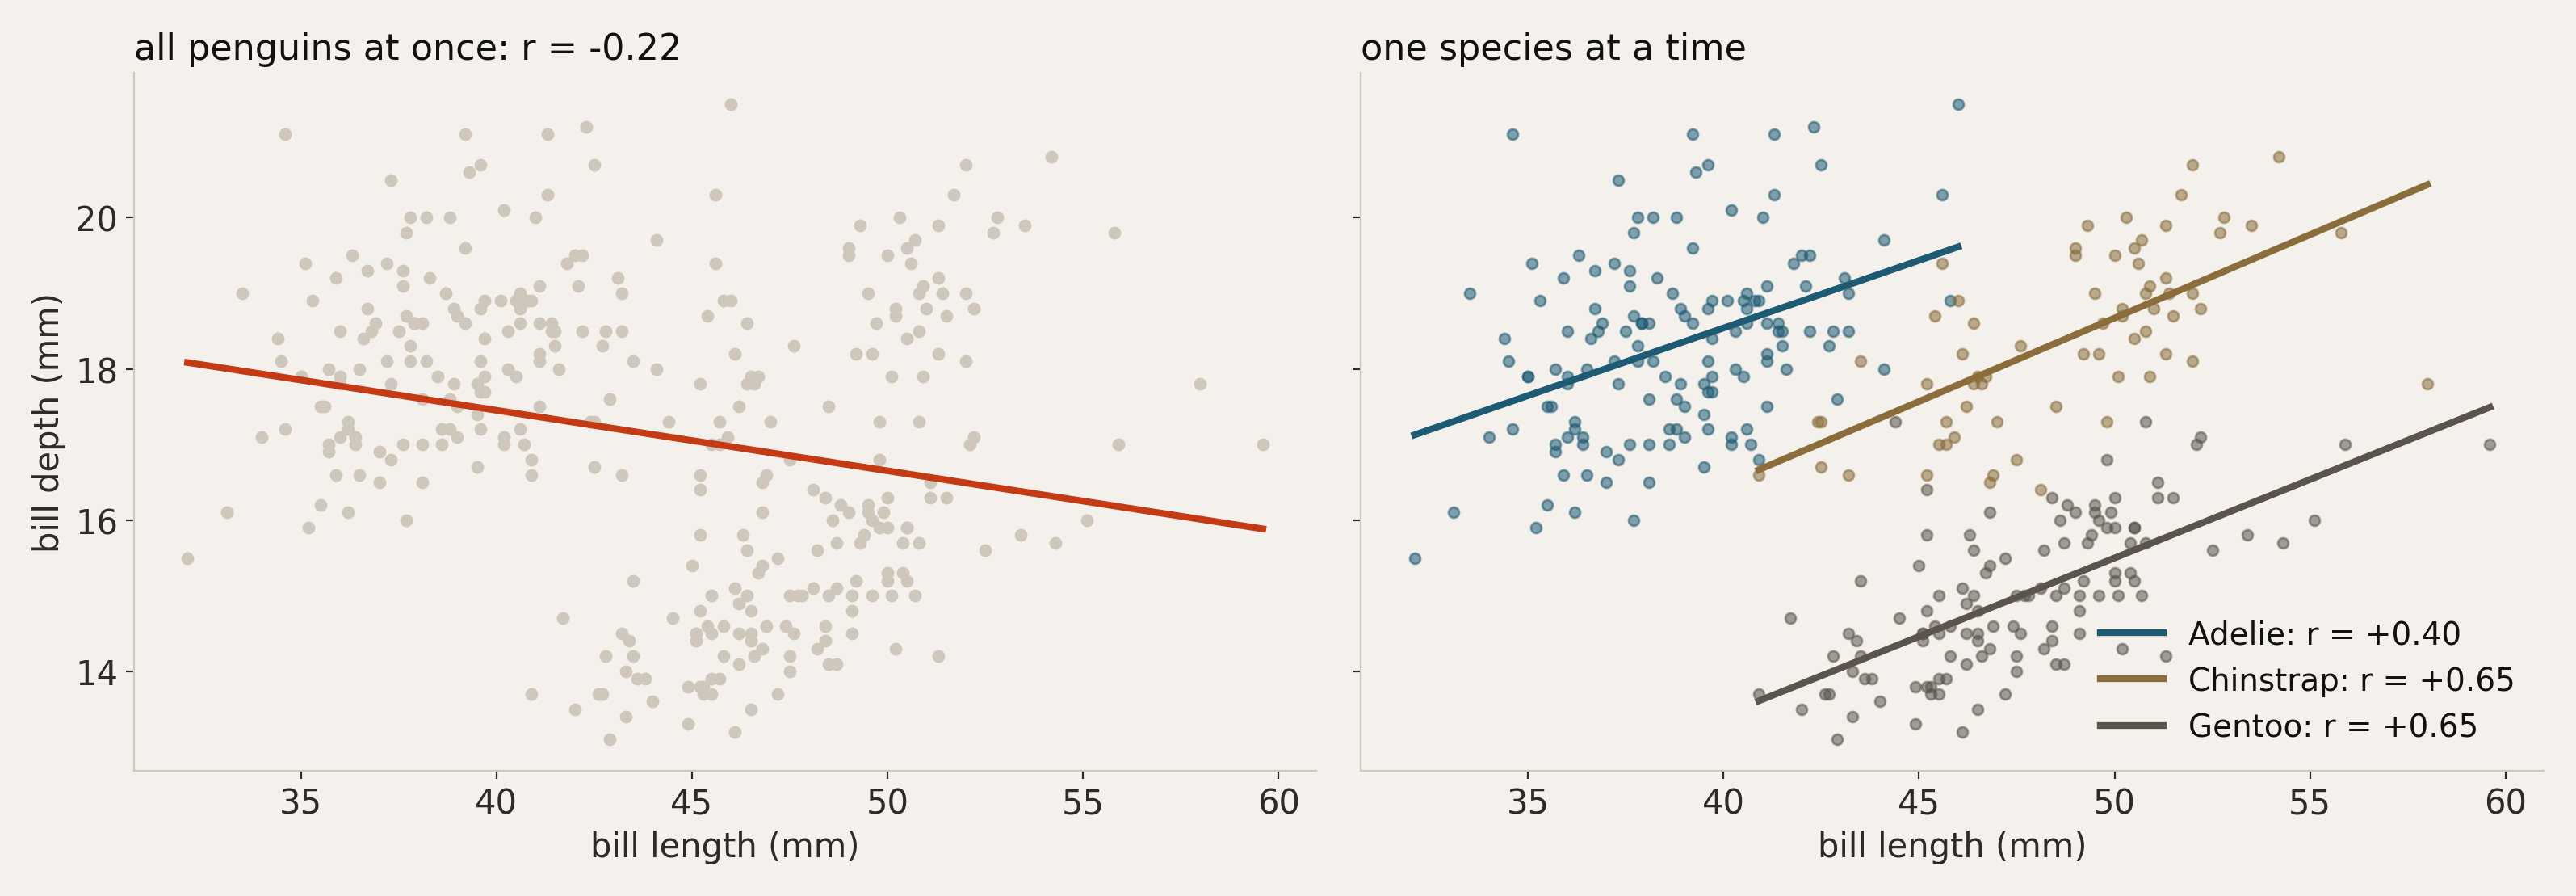
\includegraphics[width=\textwidth]{lesson5/simpson.png}
\caption{Bill length against bill depth. Left: all penguins at once. Right: one species at a time.}
\label{fig:simpson}
\end{figure}

All penguins at once: longer bills are shallower, $r = -0.22$. One species at a time: in every species a longer bill is deeper, $+0.40$ for Adelie, $+0.65$ for Chinstrap and $+0.65$ for Gentoo. Nothing about the birds changed. Gentoos have long, shallow bills and Adelies short, deep ones, which lays the three clouds along a downward diagonal; the pooled line measures the difference between species. This is Simpson's paradox, which lesson 2 met as a table of admissions. As a scatter you can see the mechanism: three clouds, and one line drawn through them. Note how easily this happens: a correlation matrix is computed on the numeric columns only, so species, island and sex are dropped before a single correlation is computed. Look at a few bills and you discover there are three kinds of penguin.

\subsubsection{Seven of fifteen correlations change sign}
Now all fifteen pairs of measurements, pooled and within species. ``Within species'' means: subtract each species' own mean from both columns, then correlate. That removes the differences between species and keeps the differences inside them.

\begin{figure}[H]
\centering
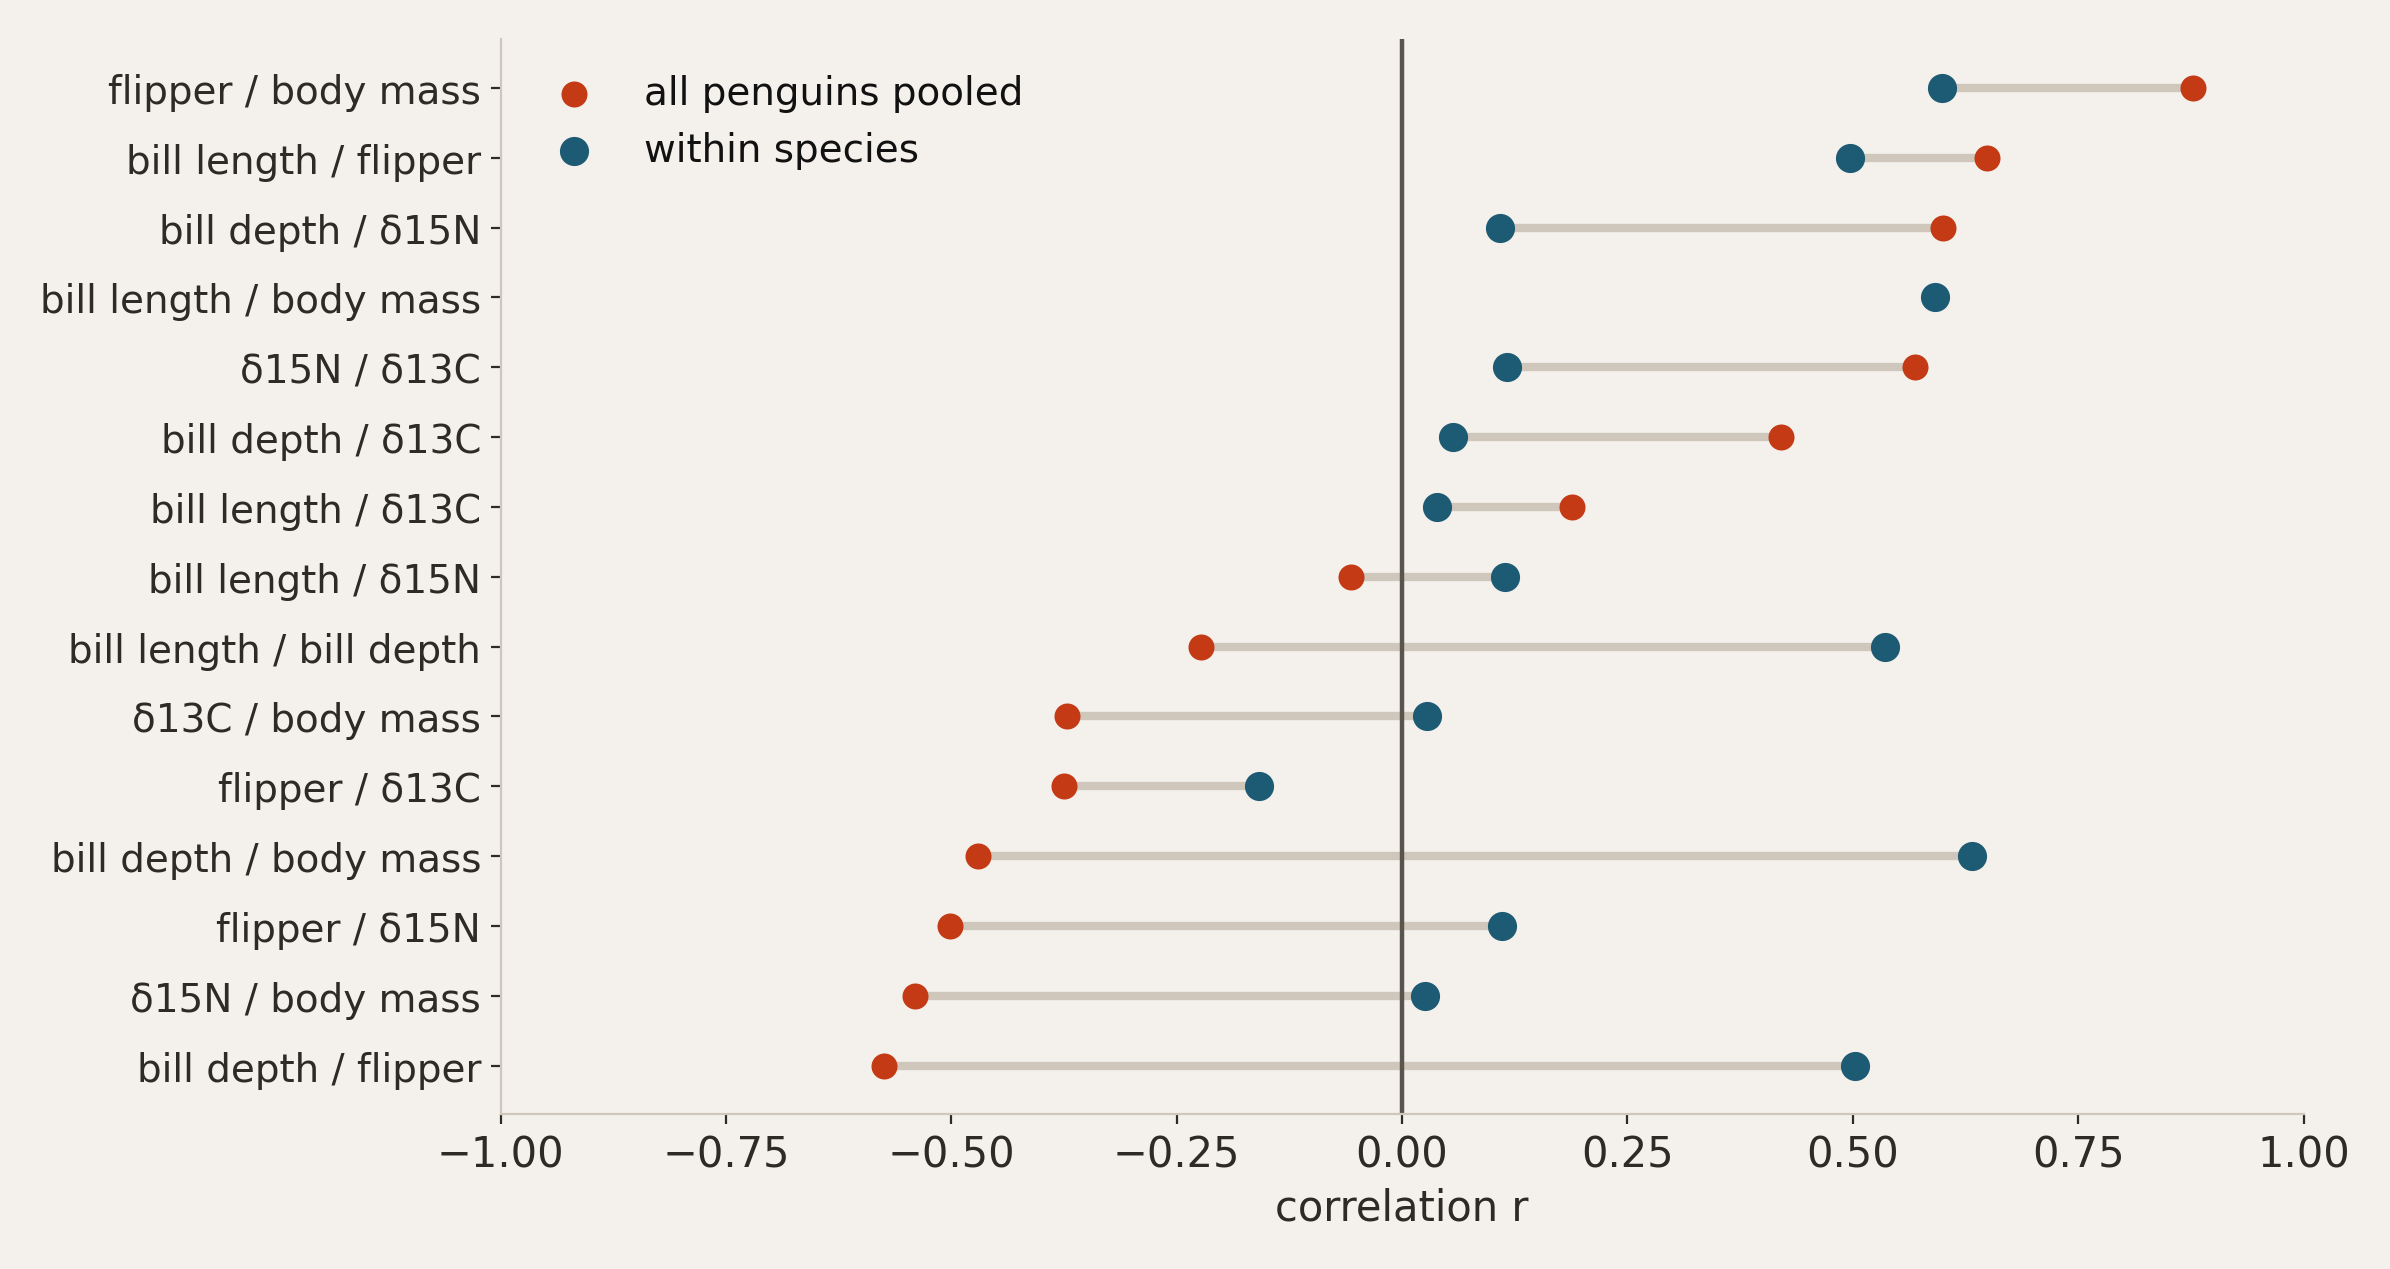
\includegraphics[width=0.85\textwidth]{lesson5/pairs.png}
\caption{Fifteen correlations. Red: all penguins together. Petrol: within species.}
\label{fig:pairs}
\end{figure}

Seven of fifteen change sign. Almost half of the claims you would make turn around when you go one level deeper. Two are worth pointing at. Nitrogen-15 and body mass: $-0.54$ pooled, a number you would report; within species $+0.03$, nothing. The correlation was not weakened by controlling for species; it was made entirely of species. $\delta^{15}$N rises with what an animal eats, and the species eat differently and happen to differ in size. Bill length and body mass: $+0.59$ pooled and $+0.59$ within. A bigger bird has a bigger bill, in every group. So the lesson is not ``distrust all correlations''.

There are three ways to handle a confounder, in increasing effort: report per group, take off the group mean first, or put the variable in a model. And then the part no method fixes: the confounder has to be in your data. If nobody had recorded the species, every number would be just as wrong, and nothing would tell you.

\subsubsection{A penalty on the weights: what L1 and L2 do}
The trick I promised. I first used it on a dataset of $150$ people with two kinds of cancer, and for each person $10{,}000$ DNA markers. The question was whether any of the markers says something about the kind of cancer. If you know a little statistics, you know that you will find patterns in $10{,}000$ features, guaranteed, just as in the $300$ hunts over the chat channel. This is the recipe for overfitting, and a correlation matrix will hand you noise. The solution was \emph{regularisation}.

First, how do you measure how wrong a model is? Suppose I am a model guessing your height. I guess $4$ metres for one person, far too high, and $20$ centimetres for the next, far too low. On average my error is close to zero, because the two errors cancel. So you square each error before averaging: both become positive, and big errors count much more than small ones. That is the \emph{mean squared error}:
$$\text{MSE} = \frac{1}{n} \sum_{i=1}^{n} (y_i - \hat{y}_i)^2,$$
with $y_i$ the real value and $\hat{y}_i$ the prediction.

A linear regression gives every feature $x_j$ a weight $w_j$, and picks the weights with the smallest error. With $100$ features and $500$ rows it will happily give every feature some weight, also the useless ones. A penalty adds a cost for large weights to the error, and $\alpha$ sets how strict it is:
$$\text{L1: } \text{MSE} + \alpha \sum_j |w_j| \qquad\qquad \text{L2: } \text{MSE} + \alpha \sum_j w_j^2.$$
Of two models that predict equally well, the one with the smaller weights wins.

\begin{figure}[H]
\centering
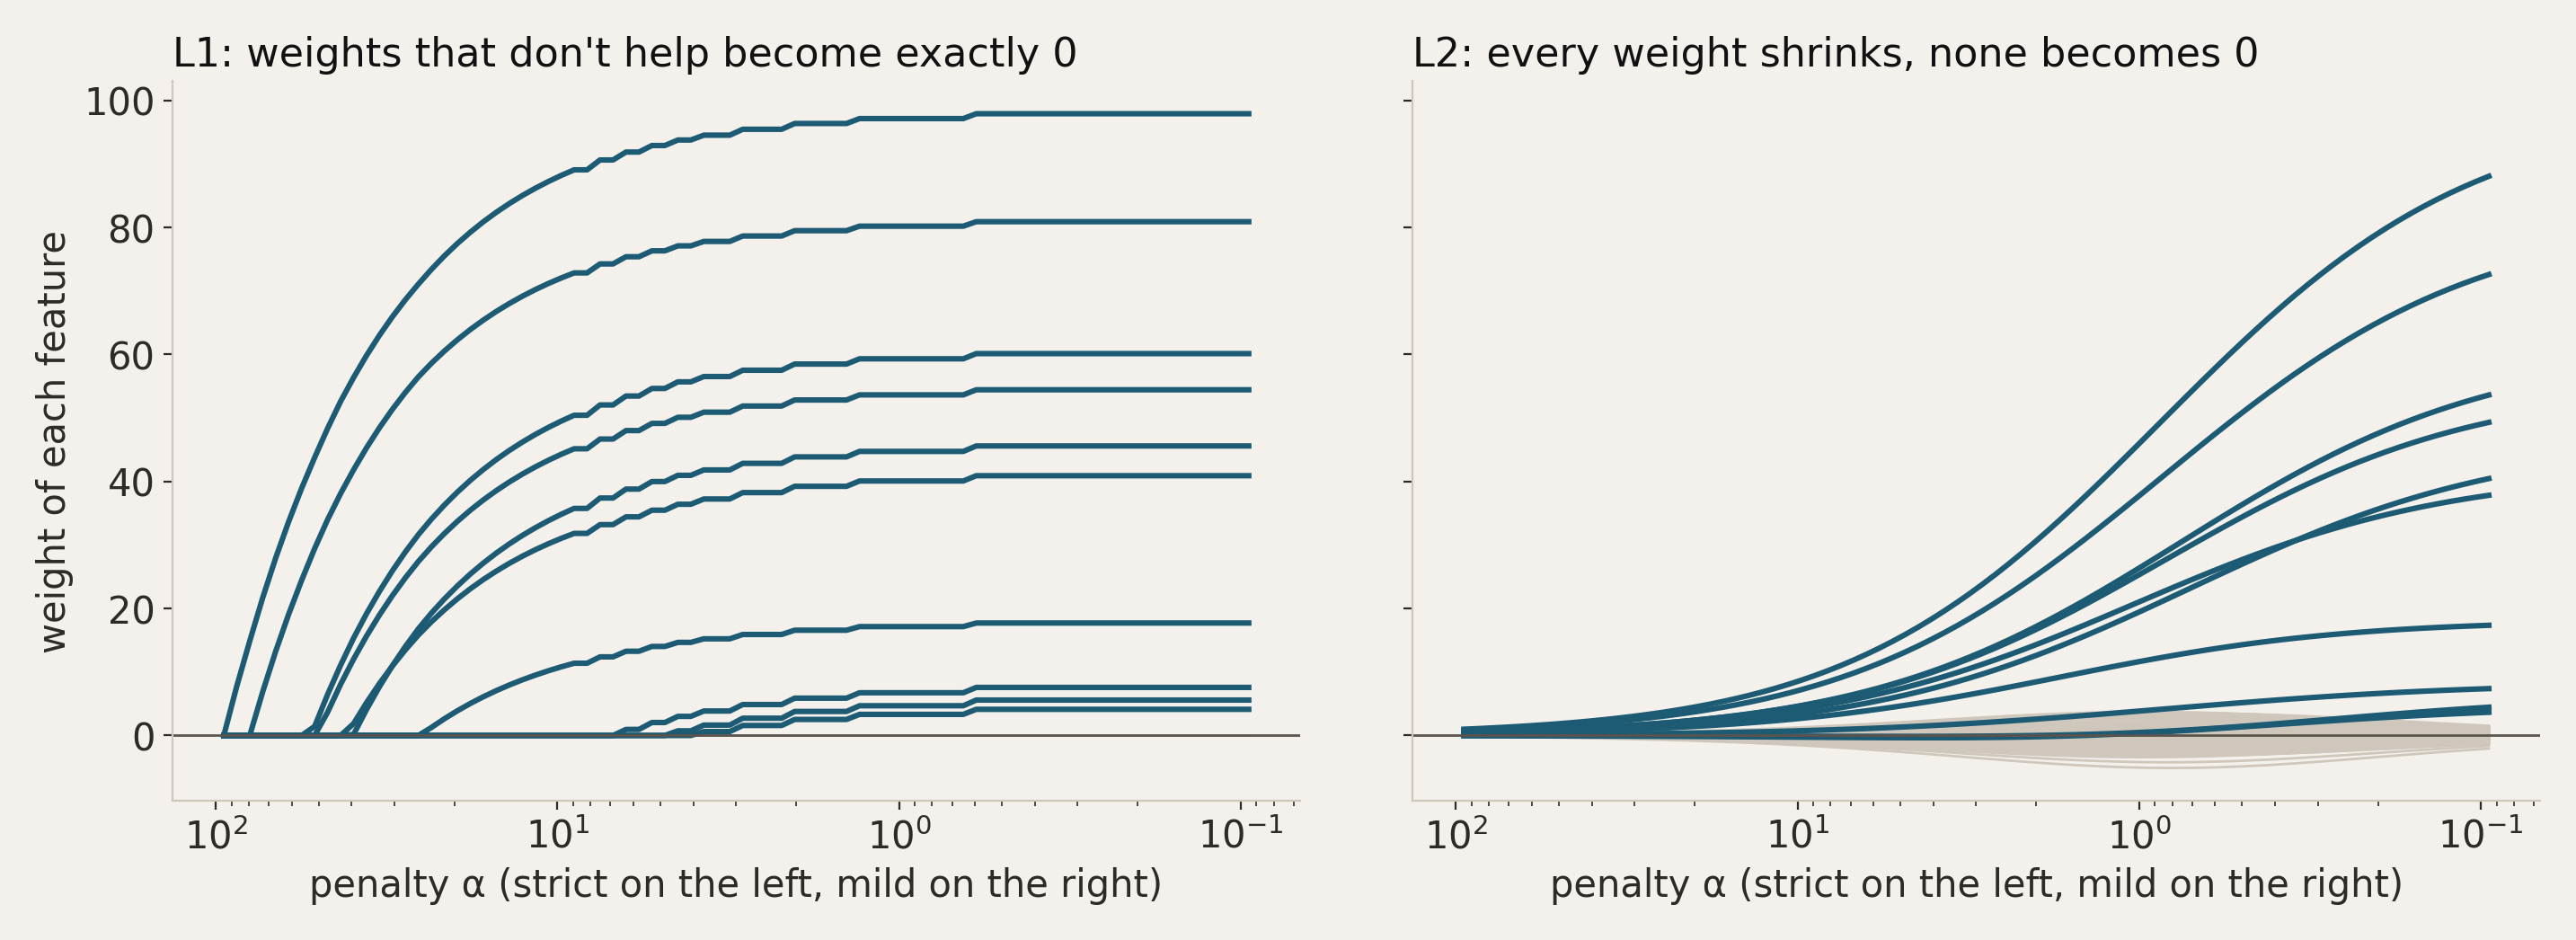
\includegraphics[width=\textwidth]{lesson5/reg_paths.png}
\caption{The weights of the same simulated data as the penalty goes from strict (left) to mild (right). Left panel: L1. Right panel: L2.}
\label{fig:reg-paths}
\end{figure}

L1 (also called \emph{lasso}) pushes the weights of features that don't help to exactly zero, and as the penalty grows, the useful ones drop out one by one, the least useful first. L2 (\emph{ridge}) shrinks every weight smoothly, but keeps them all; none ever becomes exactly zero. That is why L1 can select features: what survives the penalty is what matters. \emph{Elastic net} mixes the two, and its \texttt{l1\_ratio} says how much is L1: $1$ is pure L1, $0$ pure L2.

Two analogies from class. A meeting with a specialist in the room: on their subject, their vote may count more than the others', but not ten times as much, because then they can overrule the whole group by saying no. How much extra weight still gives good decisions? That is regularisation. Or my daughter of fourteen, going shopping for Sinterklaas presents: give her a budget, and she has to make choices, hopefully relevant ones. Squeeze the budget, and only what matters gets money; the rest goes to zero.

\subsubsection{A penalty on the weights finds the useful features}
A simulated dataset: $500$ rows and $100$ features, of which ten really matter and ninety are pure noise. Can you find the ten?

\begin{figure}[H]
\centering
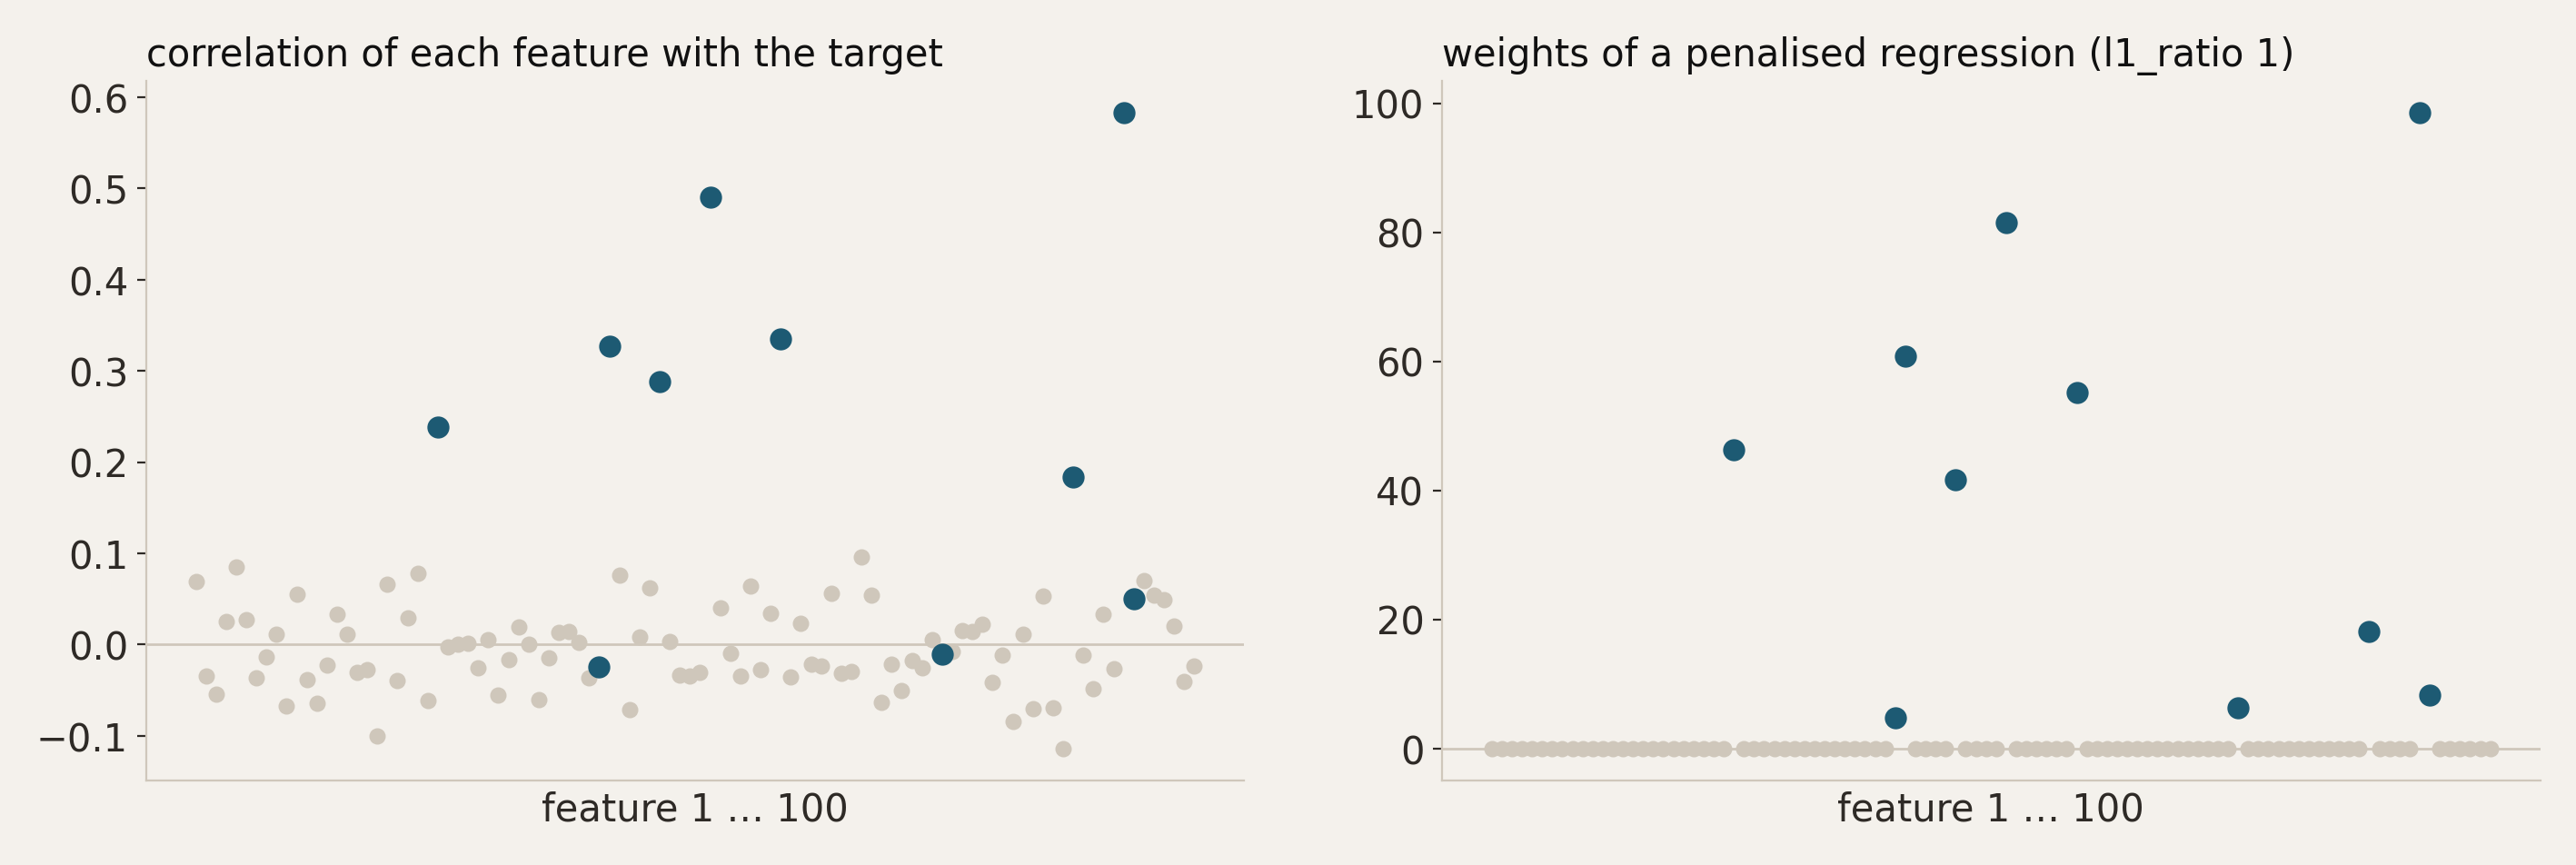
\includegraphics[width=\textwidth]{lesson5/regularisation.png}
\caption{Left: the correlation of each feature with the target. Right: the weights of a penalised regression. Petrol: the ten largest weights.}
\label{fig:regularisation}
\end{figure}

Plot each feature's correlation with the target, and six stand out; the rest looks like noise, and you can see how noisy it is. Now misuse a linear regression on purpose: the goal is not the model, it is the weights. A grid search over the strictness $\alpha$ and the mix picks pure L1, \texttt{l1\_ratio = 1}. Almost every weight is exactly zero, and the real features pop out. Three of the ten largest weights belong to features that have almost no correlation with the target on their own: a feature can matter in combination with the others while its correlation alone is near zero. The correlation matrix is well known; it is not very reliable. (The grid search is a preview: hyperparameters are next semester's topic.)

\againconcretely
Pooled, longer bills are shallower. Within every species they are deeper. Same birds, opposite sentence. Before you report a correlation, ask what else is different between the groups you compare. The confounder has to be in your data: species was, and one \texttt{groupby} fixed it. If nobody had recorded it, nothing would tell you. With many features, let a penalised regression do the selecting, and read its weights.

% ─────────────────────────────────────────────
\subsection{Can you recognise someone by how they type?}
\label{sec:typing}
The last question takes one claim all the way through: \emph{people are more identifiable by how they write than by what they write about}. The mechanism is plausible, and it predicts something specific: habits should be stable, while subjects drift. Three warnings go with it. Accuracy only tells you there is something to look at; it is not the finding. The weights tell you what the model learned: a habit, or just a topic. And count the right thing: $218{,}670$ messages, but eight people. For a claim about people, $n$ is eight. A model that works can still be right for the wrong reason; a stopped clock gives the right time twice a day.

\subsubsection{47\% right, but why?}
A model reads one message from the eight most active people in the channel and guesses who wrote it: tf-idf over all words and a logistic regression. It is right $47\%$ of the time. What is the baseline? Not one in eight, because some people write much more than others. The simplest honest model always guesses the busiest person, and is right $22\%$ of the time. So $47\%$ is twice the baseline: a gate passed, not a destination. Half the messages still go to the wrong person. What did the model learn? That is in its weights.

\begin{table}[H]
\centering
\begin{tabularx}{\textwidth}{@{}l X l@{}}
\toprule
\textbf{Person} & \textbf{Words the model leans on} & \textbf{What that is} \\
\midrule
ali1234 & n900, pidgin, qml, mythtv & subject matter \\
MartijnVdS & dimpy, mungbean, neuro & other people's nicknames \\
zmoylan-pi & ireland, dublin & where he lives \\
daftykins & 0o, xd, hrmm & typing \\
popey & dont, didnt, thats & typing: no apostrophes \\
\bottomrule
\end{tabularx}
\caption{The strongest words per person in the one-message model.}
\label{tab:weights}
\end{table}

Read them, and they are not all the same kind of thing. Devices and software are a topic. Other people's nicknames are not a writing habit but a social position: who you talk to. Ireland and Dublin are where someone lives. Only the last two are about how someone types. The rest is a topic detector wearing a stylometry costume, and a topic detector fails the moment someone changes the subject, stops talking to Dimpy, or moves house. That is exactly the situation an authorship model is for. When a model works, read its weights and ask what each one really is.

\subsubsection{Three ways to write a smiley, and nobody mixes them}
So stop using the model to find the fingerprint, and measure the habits directly. Nothing here needs machine learning: five \texttt{RegexFeature} steps and a \texttt{groupby}, the same transform you used in lesson 1 for URLs, now pointed at smileys and apostrophes.

\begin{figure}[H]
\centering
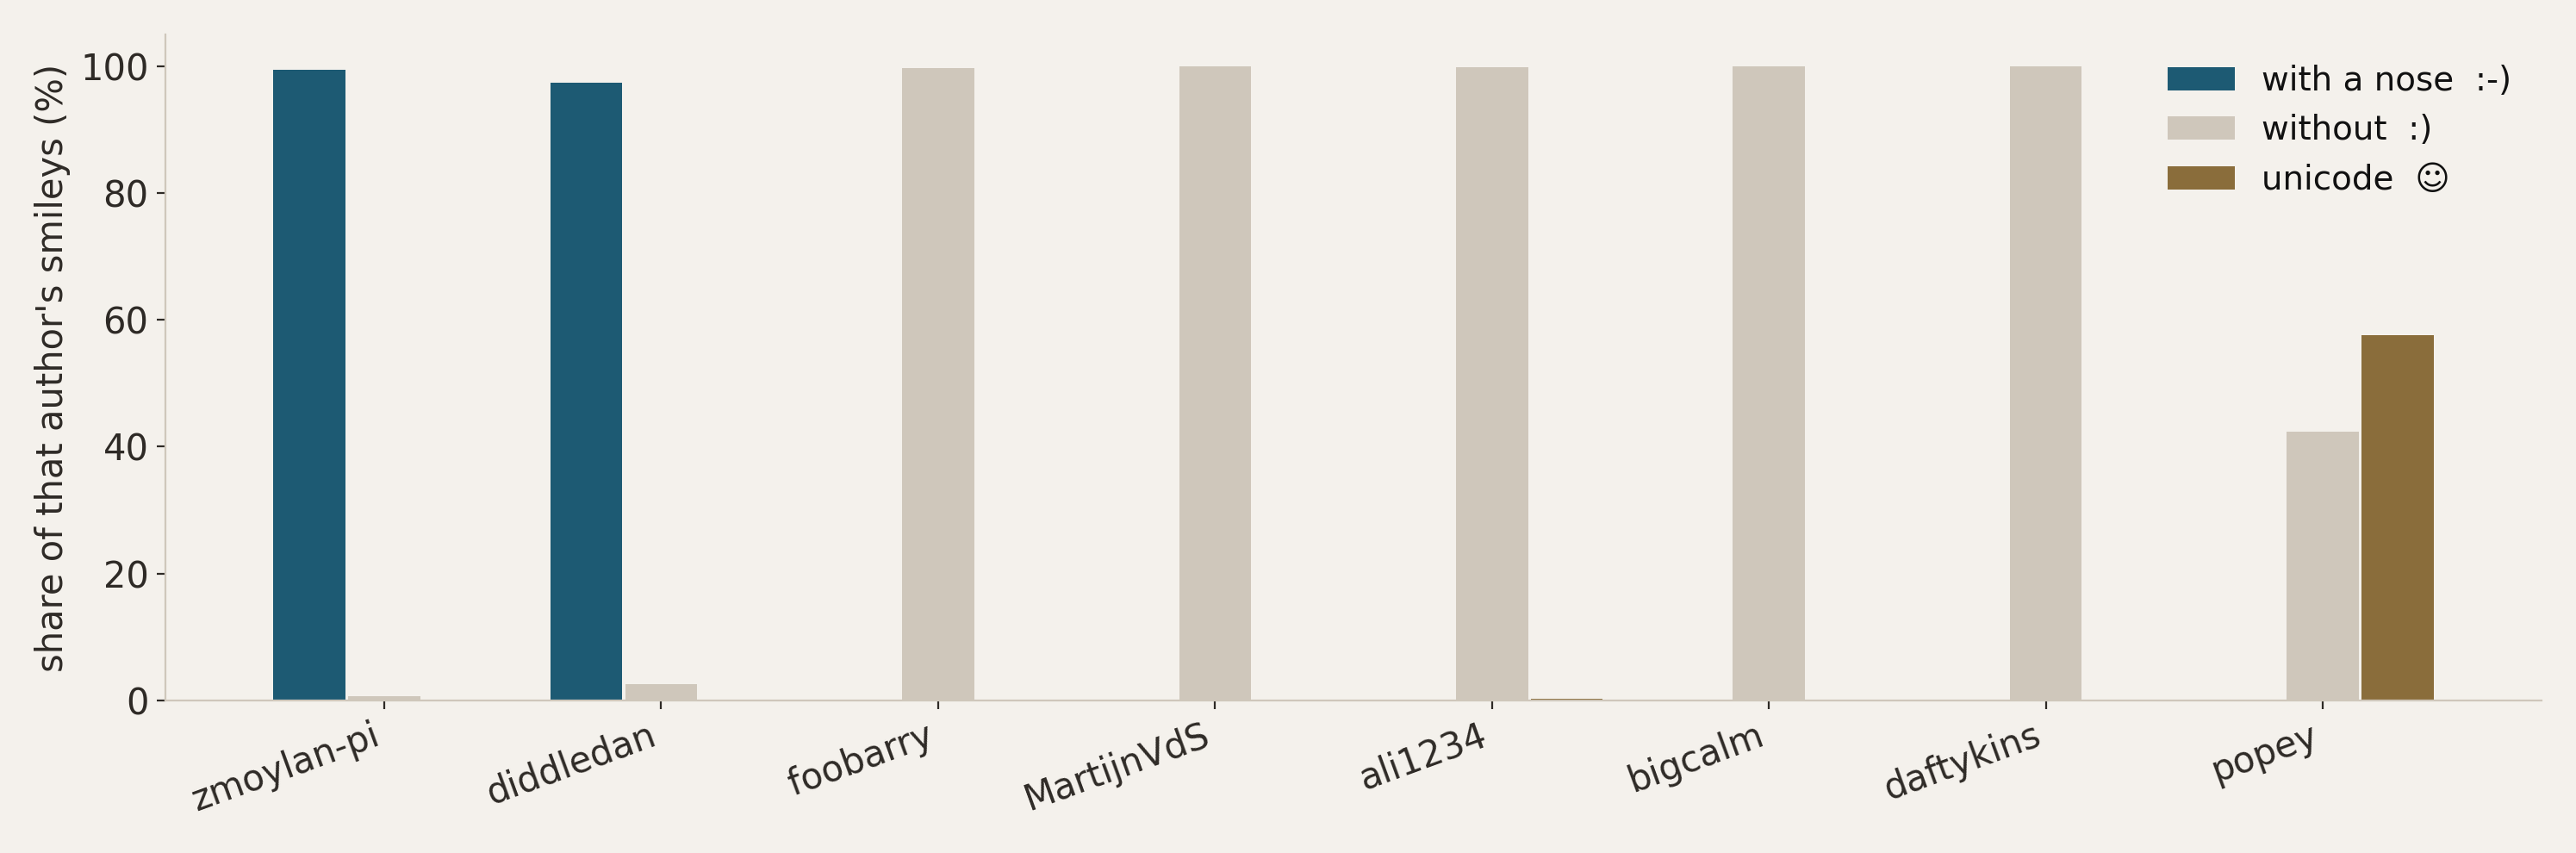
\includegraphics[width=\textwidth]{lesson5/smileys.png}
\caption{Smileys with a nose \texttt{:-)}, without \texttt{:)}, and the unicode smiley (U+263A), per person.}
\label{fig:smileys}
\end{figure}

Smileys come in three dialects, and nobody mixes them. Two people use the nose almost every time; five never do; there is nobody in between. popey writes the unicode smiley, which nobody else types. Most differences between people are a matter of degree. This one is a choice, made once and kept for years, by people who read each other's messages every day. Apostrophes, capitals, addressing someone by name and posting at night look the same: a couple of people at one extreme, everyone else at the other. There is no typical author in this channel.

\subsubsection{Fifty messages at a time: ten habits do what 17,918 words do}
If the habits are this decisive, why only $47\%$? Because of the unit of analysis. Three quarters of all messages carry no habit at all: ``ok'', ``thanks'', ``brb''. Nobody can tell from ``ok'' who wrote it, so a model reading one message usually has nothing to go on; $47\%$ is what a strong signal looks like when it is sparse. So stop asking about one message: pool fifty messages per person into a block. That needs a small pipeline step of our own, \texttt{BlockMessages}, because what counts as one row is a decision worth naming.

\begin{figure}[H]
\centering
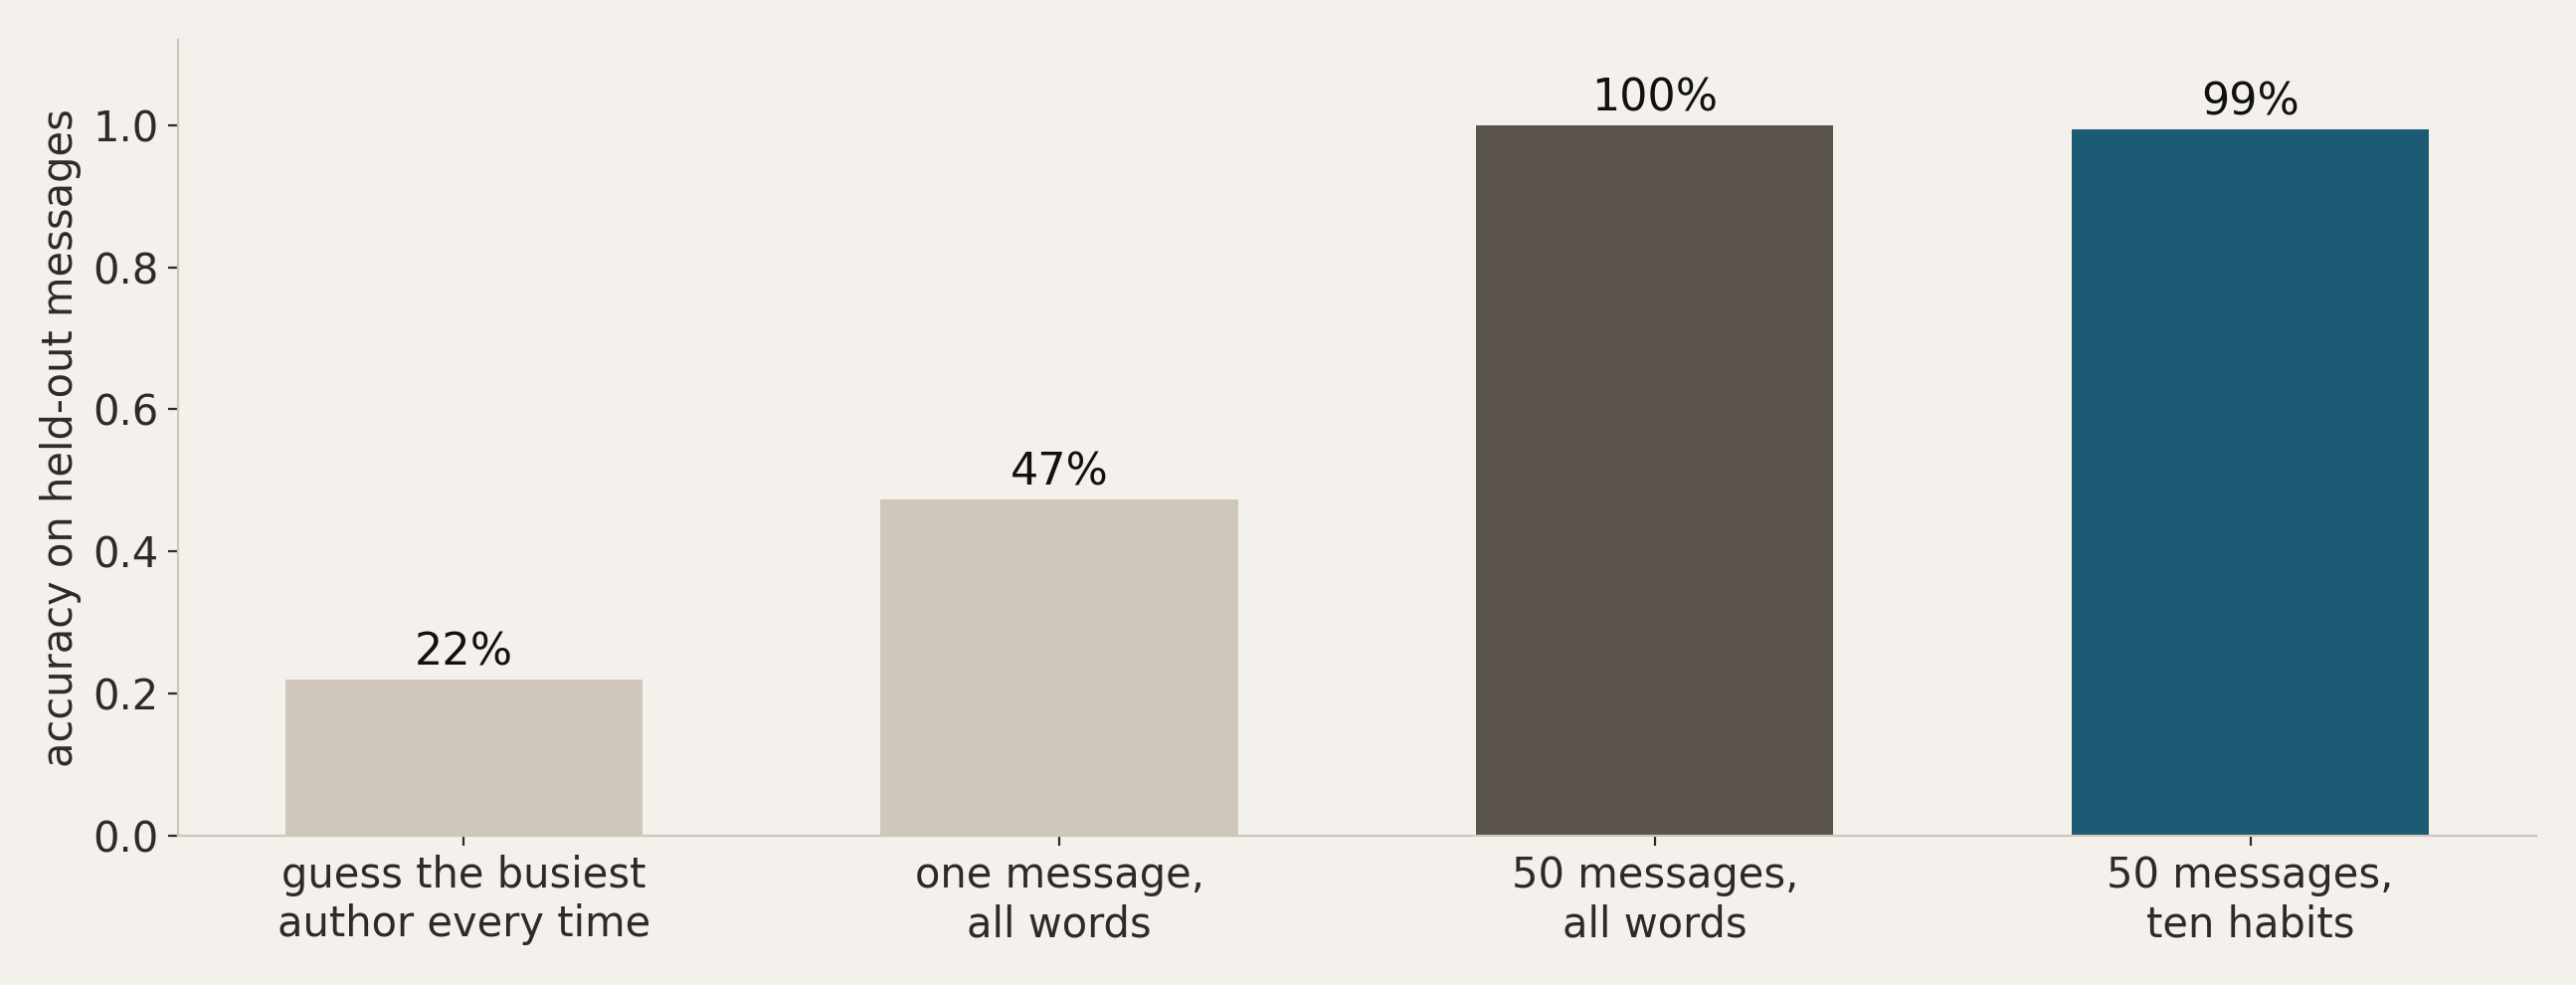
\includegraphics[width=\textwidth]{lesson5/blocks.png}
\caption{Accuracy on held-out messages, for four ways of guessing the author.}
\label{fig:blocks}
\end{figure}

Then race two models on the same $4{,}368$ blocks. One knows every word, $17{,}918$ of them, and gets $100\%$. The other knows ten habits and nothing else, and gets $99\%$. The one with no topics, no nicknames and no place names is within a point of the one that knows everything. And its ten weights can be read aloud: MartijnVdS is addressing people, daftykins is noseless smileys at night, foobarry is recognised by never posting at night.

Which is the better model? In class someone defended the big one: test it on a held-out set, a thousand times if you like, and if it scores $100\%$ against $99\%$, take the $100\%$. I don't think a train-test split saves it, because the data changes over time, and the student named the reason themselves: other words, and other people who also mention Ireland one day. Someone who moves or stops talking to Dimpy breaks their own feature, and for Dublin and Ireland that is to be expected, not exceptional. The $17{,}918$ words bring an enormous amount of noise into the model for one extra percent: they score $100\%$ today, and after a year in production the model drifts away, and then the verdict is ``your model doesn't work''. I can't prove that here; it is an intuition. But if we made this bet a hundred times, I would put my money on the ten habits every time, and you would need a lot more analysis to convince me otherwise. Sometimes there is no simple model, and then a complex one is very useful and you accept its noise. When there is a choice between ten features at $99\%$ and $17{,}918$ at $100\%$, take the ten. Another suggestion from the room fits the whole lesson: start with two habits and add them one at a time, instead of starting at the maximum.

\subsubsection{The same eight people, four years later}
The third leg: does it hold where nobody looked? Fit nothing; measure the same habits in 2013--2014 and again in 2016--2017.

\begin{figure}[H]
\centering
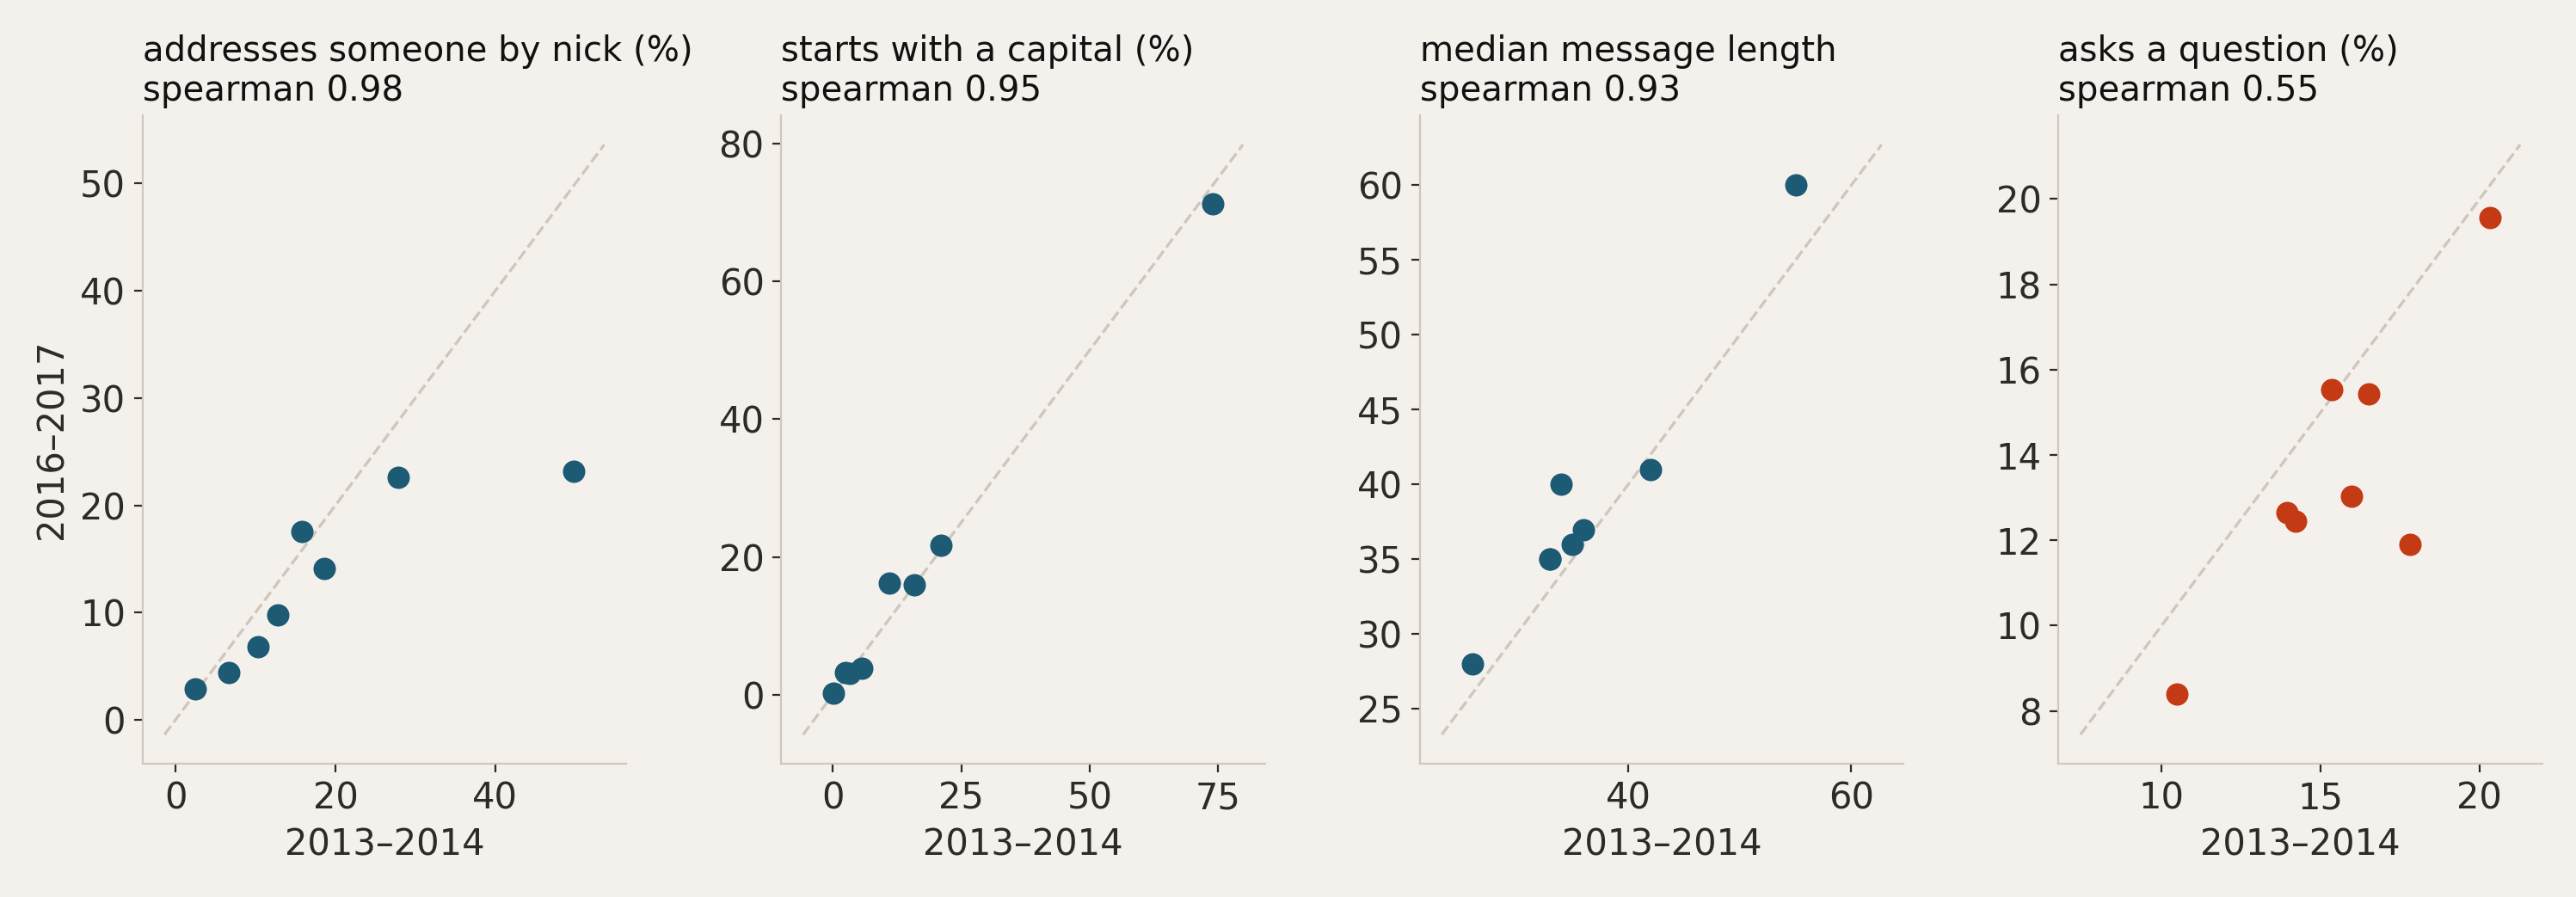
\includegraphics[width=\textwidth]{lesson5/stability.png}
\caption{Each dot is one person: a habit in 2013--2014 against 2016--2017. On the diagonal means unchanged.}
\label{fig:stability}
\end{figure}

Addressing people by name, starting with a capital, message length: the order of the eight hardly changes, with Spearman correlations of $0.93$ to $0.98$ after a four-year gap. If you started $75\%$ of your messages with a capital in 2013, you still do in 2016. Two people became a little more long-winded, and one addresses people less than before, but the habits stay. That is replication, and it explains why ten habits are enough for $99\%$. Asking questions does move (Spearman $0.55$), and drops over time: whether you ask questions depends on whether you have a problem right now. That is not a weakness of the finding. A measure that could say no makes the others believable, because it shows the measurement could have failed.

\againconcretely
Ten habits recognise eight people, four years apart. But it is eight people. Through the grid of question four, this claim lands in the best cell: a model that fits, a mechanism, replication. How strong is eight out of eight? If staying stable were a coin flip, all eight would stay stable with probability $(1/2)^8 = 1/256$: a fairly strong signal. But $218{,}670$ messages don't make $n$ bigger. The claim is about people, so $n = 8$, and large data does not fix a small $n$: a hundred people with fifty thousand messages would say much more. These habits might be specific to Linux users; children, teenagers and twenty-five-year-olds, or writers in the UK, Ukraine, South Africa or on a Chinese keyboard, might behave differently. The fix is cheap: the habits run on anyone with thirty messages, so recompute the stability for everyone with enough history in both periods. The accuracy was a gate; the weights were the finding. Reported honestly: among the eight most active people, ten habits classify blocks of fifty messages at $99\%$, stable over four years. Others: untested.

% ─────────────────────────────────────────────
\subsection{The six questions, answered}
\label{sec:lesson5-summary}
\begin{table}[H]
\centering
\begin{tabularx}{\textwidth}{@{}l X@{}}
\toprule
\textbf{Question} & \textbf{Answer} \\
\midrule
What is a model? & A simplification you choose. Not true, not objective, useful for what it leaves out. \\
Why keep a model simple? & You can only understand simple shapes, and a model that fits anything tells you nothing. \\
How do you build a model? & Look, think, add one step or one term. Then read the residual. \\
When should you believe a pattern? & When it beats chance, has a mechanism, and shows up where you didn't look. \\
What can a correlation hide? & The variable you left out. It has to be in your data. \\
Can you recognise someone by how they type? & These eight people, yes. Large data does not fix a small $n$. \\
\bottomrule
\end{tabularx}
\end{table}

Notebooks 05.1 to 05.5 work through the questions: 05.1 the line as a claim, the hunt and the three legs; 05.2 correlation and Simpson's paradox; 05.3 the COVID model as a question you answer yourself, and 05.4 the worked answer and the script; 05.5 how people type. In your own chat: pick a habit you can write as a regex, measure it per person, and report $n$ at the level of your claim.
\newpage

\section{Reading code with atlas}
\label{sec:atlas}
This course asks two things of your code. It has to make the plots in your report, and you have to be able to explain how it does that: in the final assignment you show me a picture of your code and walk me through it. This section explains why I ask for a picture and not for the code itself, and what atlas, the tool that draws the picture, shows you. The argument is the same one this course makes about data: a good visualisation lets you see in a second what a table of numbers hides, and code is no different.

% ─────────────────────────────────────────────
\subsection{The problem with reading a lot of code}
\label{sec:atlas-reading}
Until recently, writing code was the slow part. Reading it kept up, because a person can only write so much in a day. With a coding agent that balance is gone. An agent writes a function in seconds, a feature in minutes, and several agents can work on several projects at once. Somebody still has to look at all of it and decide whether it is any good: you, for your own project; a senior developer, for a team (figure~\ref{fig:atlas-agents}). Writing has become cheap. Reading has not.

\begin{figure}[H]
\centering
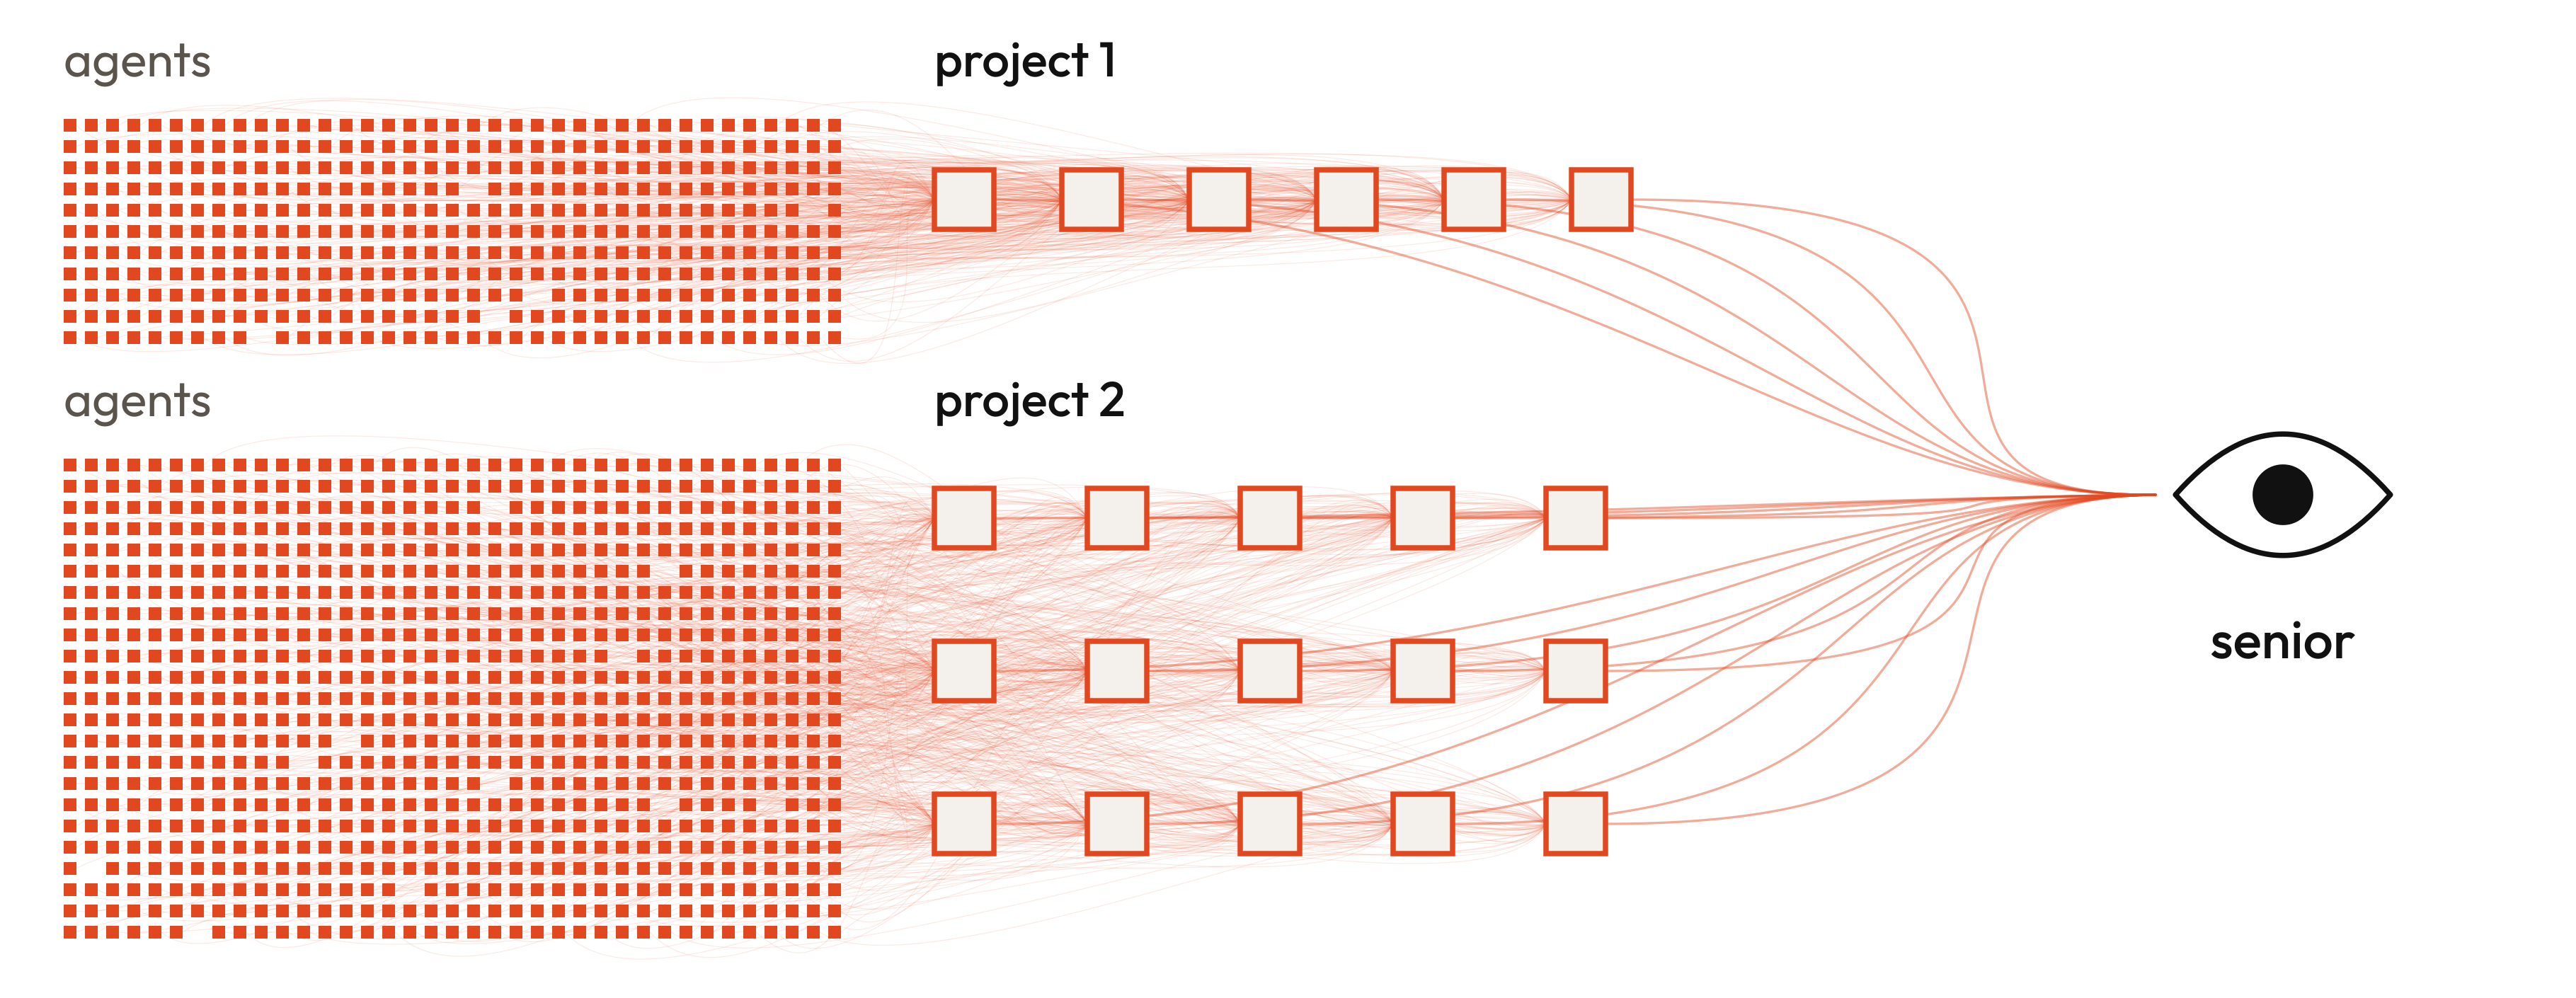
\includegraphics[width=\textwidth]{atlas/agents.png}
\caption{Many agents, a few projects, one person who has to oversee all of it.}
\label{fig:atlas-agents}
\end{figure}

Put the times next to each other (figure~\ref{fig:atlas-timeline}). Reading one function carefully takes about a minute. Reading one pull request, a single proposed change, takes the better part of an hour. Reading the $179$ commits an agent can produce in a project takes a day, and by then there are more. And all of that only tells you what each piece does. What you actually want to know is something no single line tells you: how the pieces fit together. To see that from the code, you have to read it all and build the structure in your head, one line at a time.

\begin{figure}[H]
\centering
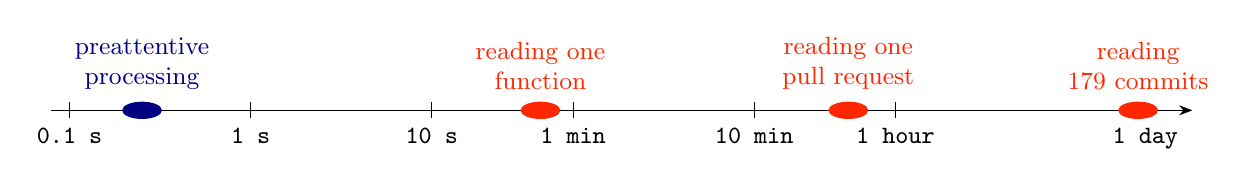
\begin{tikzpicture}[x=2.3cm, every node/.style={font=\small}]
  % log10 seconds: 0.1 s = -1, 1 s = 0, 10 s = 1, 1 min = 1.78, 10 min = 2.78, 1 h = 3.56, 1 day = 4.94
  \draw[-{Stealth}] (-1.1,0) -- (5.2,0);
  \foreach \x/\l in {-1/{0.1 s}, 0/{1 s}, 1/{10 s}, 1.78/{1 min}, 2.78/{10 min}, 3.56/{1 hour}, 4.94/{1 day}}
    \draw (\x,0.1) -- (\x,-0.1) node[below] {\texttt{\l}};
  \fill[blue!50!black] (-0.6,0) circle (0.11) node[above=4pt, align=center] {preattentive\\processing};
  \fill[red!70!orange] (1.6,0) circle (0.11) node[above=4pt, align=center] {reading one\\function};
  \fill[red!70!orange] (3.3,0) circle (0.11) node[above=4pt, align=center] {reading one\\pull request};
  \fill[red!70!orange] (4.9,0) circle (0.11) node[above=4pt, align=center] {reading\\179 commits};
\end{tikzpicture}
\caption{How long it takes to see something, against how long it takes to read it. The axis is logarithmic: every tick is ten times longer.}
\label{fig:atlas-timeline}
\end{figure}

There is a second problem: the output does not tell you whether the code was good. Take a program that fetches the monthly sunspot counts since 1749 from the web, keeps them as a CSV file, takes the mean over thirteen months and draws both (figure~\ref{fig:atlas-sunspots}). I wrote two programs that make exactly this figure: one a sloppy script, one typed and tidy. The figure cannot tell them apart. Neither can your tests: they check that the figure comes out, not how. And neither can a linter: ruff and ty look at lines and types, and every line of the sloppy script can be fine on its own. What is wrong with it is the way the lines are connected.

\begin{figure}[H]
\centering
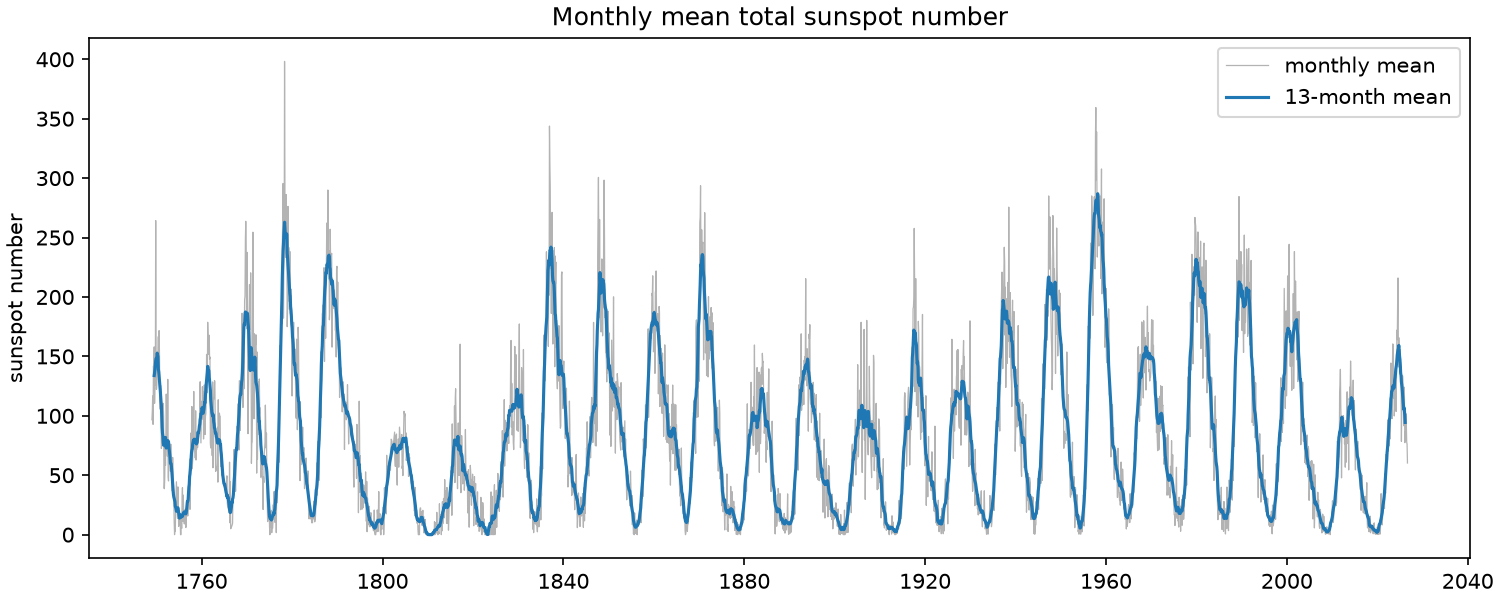
\includegraphics[width=0.8\textwidth]{atlas/sunspots.png}
\caption{The monthly sunspot number since 1749, with its 13-month mean. Two very different programs make exactly this figure.}
\label{fig:atlas-sunspots}
\end{figure}

\subsubsection{Bad code is a shape}
What makes code hard to maintain is rarely one bad line. It is a shape: the way the pieces depend on each other. Figure~\ref{fig:atlas-shapes} shows three.

\begin{figure}[H]
\centering
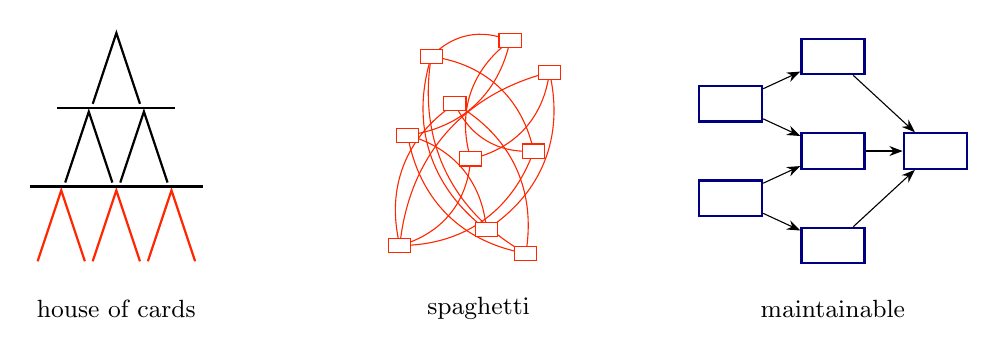
\begin{tikzpicture}[every node/.style={font=\small}]
  % house of cards
  \begin{scope}[xshift=0cm]
    \foreach \x in {0,1,2} {\draw[red!70!orange, thick] (\x*0.7,0) -- (\x*0.7+0.3,0.9) -- (\x*0.7+0.6,0);}
    \draw[thick] (-0.1,0.95) -- (2.1,0.95);
    \foreach \x in {0,1} {\draw[thick] (0.35+\x*0.7,1.0) -- (0.35+\x*0.7+0.3,1.9) -- (0.35+\x*0.7+0.6,1.0);}
    \draw[thick] (0.25,1.95) -- (1.75,1.95);
    \draw[thick] (0.7,2.0) -- (1.0,2.9) -- (1.3,2.0);
    \node at (1.0,-0.6) {house of cards};
  \end{scope}
  % spaghetti
  \begin{scope}[xshift=4.6cm]
    \foreach \i/\x/\y in {1/0/0.2, 2/1.6/0.1, 3/0.4/2.6, 4/1.9/2.4, 5/0.9/1.3, 6/0.1/1.6, 7/1.7/1.4, 8/1.1/0.4, 9/0.7/2.0, 10/1.4/2.8}
      \coordinate (s\i) at (\x,\y);
    \foreach \a/\b in {1/4,1/9,2/3,2/6,3/7,4/5,5/10,6/8,7/1,8/3,9/2,10/6,5/1,4/8,3/10,7/9}
      \draw[red!70!orange, thin] (s\a) to[bend left=35] (s\b);
    \foreach \i in {1,...,10} \draw[red!70!orange, fill=white] ($(s\i)+(-0.14,-0.09)$) rectangle ($(s\i)+(0.14,0.09)$);
    \node at (1.0,-0.6) {spaghetti};
  \end{scope}
  % maintainable
  \begin{scope}[xshift=8.8cm]
    \foreach \n/\p in {a/{(0,2.0)}, b/{(0,0.8)}, c/{(1.3,2.6)}, d/{(1.3,1.4)}, e/{(1.3,0.2)}, f/{(2.6,1.4)}}
      \node[draw=blue!50!black, thick, minimum width=0.8cm, minimum height=0.45cm] (\n) at \p {};
    \foreach \a/\b in {a/c,a/d,b/d,b/e,c/f,d/f,e/f}
      \draw[-{Stealth}] (\a) -- (\b);
    \node at (1.3,-0.6) {maintainable};
  \end{scope}
\end{tikzpicture}
\caption{Three shapes code can have.}
\label{fig:atlas-shapes}
\end{figure}

A \emph{house of cards} stands, until you touch it: every layer rests on the one below, and changing a card at the bottom brings everything above it down. \emph{Spaghetti} is code where everything reads and changes everything else, so that nobody can say what a change in one place does elsewhere. \emph{Maintainable} code has a direction: data comes in, goes through named steps that each take something and give something, and comes out. You can replace one step without touching the others. Notice that none of these is a property of a line. They are properties of the connections, and connections are exactly what you lose when you read code line by line.

\subsection{Why a picture works better}
\label{sec:atlas-seeing}
Look at figure~\ref{fig:atlas-preattentive}. You found the red square before you had decided to look for it. That is \emph{preattentive processing}, which we used in lesson 5 to spot the weekly cycle in the COVID data: in the first fraction of a second, before you read anything, your visual system has already picked out what stands out. It does that for the whole field at once, so it takes the same time with $160$ squares as with $10$.

\begin{figure}[H]
\centering
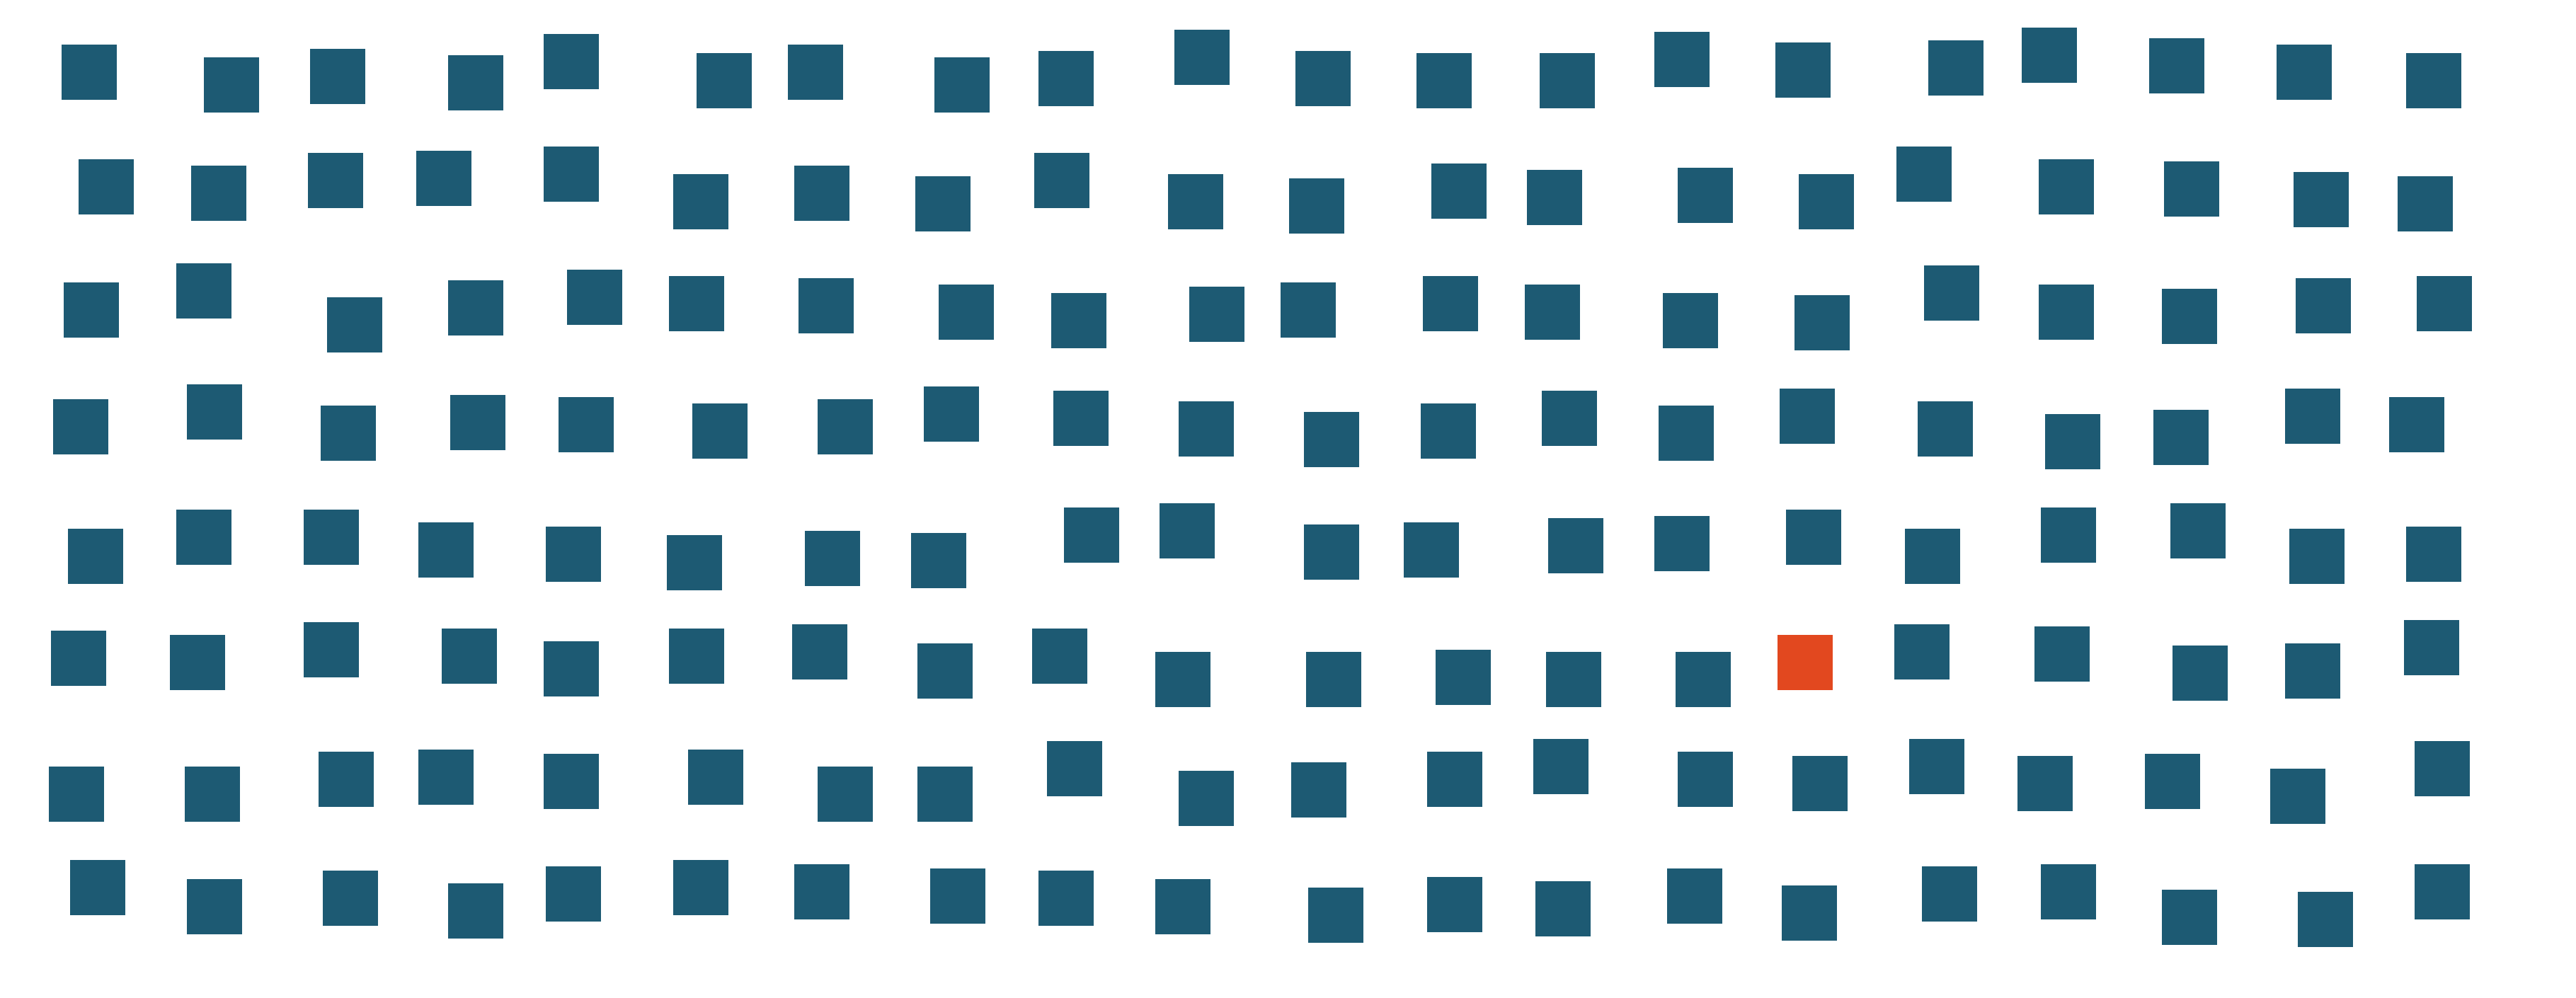
\includegraphics[width=0.8\textwidth]{atlas/preattentive.png}
\caption{One square is not like the others.}
\label{fig:atlas-preattentive}
\end{figure}

Reading works the other way. You read in series, one word after another, and the time grows with the amount of text: twice the code, twice the reading. Seeing works in parallel. That is the difference between the blue dot and the red dots in figure~\ref{fig:atlas-timeline}, and it is the whole reason this course exists: a good plot shows in half a second what a table of numbers hides. So if the structure of your code is what you want to judge, turn the structure into a picture, and let your eyes do what they are good at: spotting the box that does not belong, the arrow that goes back, the place everything points to.

% ─────────────────────────────────────────────
\subsection{What atlas draws}
\label{sec:atlas-draws}
Atlas\footnote{\url{https://github.com/raoulg/atlas}. The tour at \url{https://raoulg.github.io/atlas/} shows every step on a real example.} reads your code and draws it as two kinds of thing. \emph{Places} are where data rests: a value in memory (a DataFrame, a \texttt{Settings} object), a file on disk, a table in a database, a page on the web, a program that runs, the screen, or a global variable that a module keeps. \emph{Functions} are what carries data from one place to the next. A \emph{route} is what one entry point does, a command you run for instance, drawn from left to right: what it finds on the left, what it leaves on the right, and the functions in between, in the order they run.

Under the picture is a small piece of mathematics. The places are the objects of a category, the functions are its arrows, and composing arrows is calling one function after another; a route is the composite from an entry point to the places it reaches. One idea from that mathematics matters for how you read the picture: what a function does to the world belongs to the function. A file it writes is as much a part of what it gives as a value it returns, and a file it reads is as much a part of what it takes as a parameter. A function that quietly writes a file, or reads a global, shows that on the picture, even though its signature doesn't.

\subsubsection{The same figure from two very different programs}
Here are the two sunspot programs, as atlas draws them.

\begin{figure}[H]
\centering
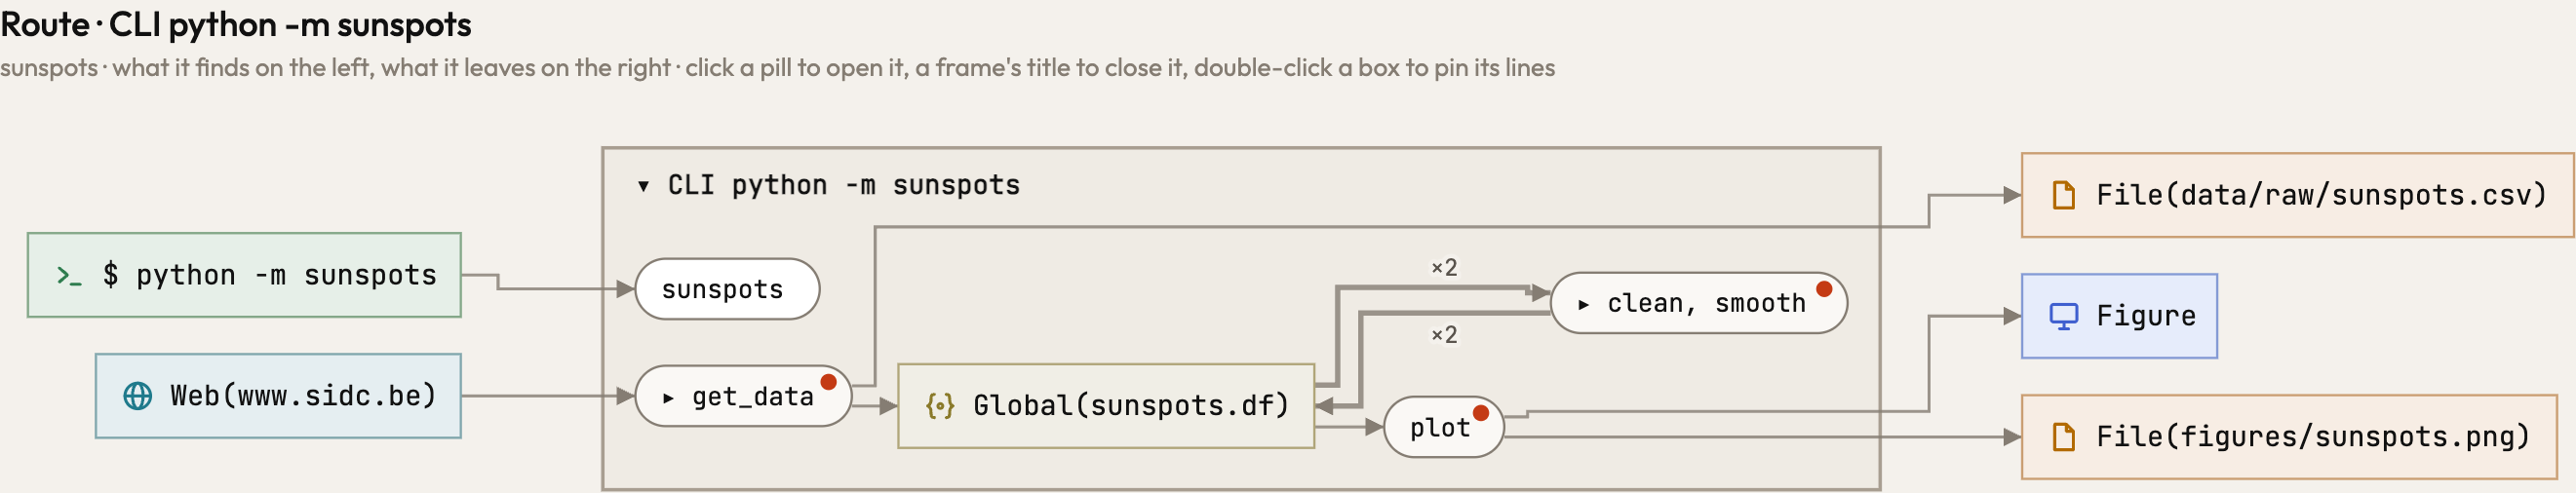
\includegraphics[width=\textwidth]{atlas/python-sloppy.png}
\caption{The sloppy script, drawn by atlas.}
\label{fig:atlas-sloppy}
\end{figure}

\begin{figure}[p]
\centering
\rotatebox{90}{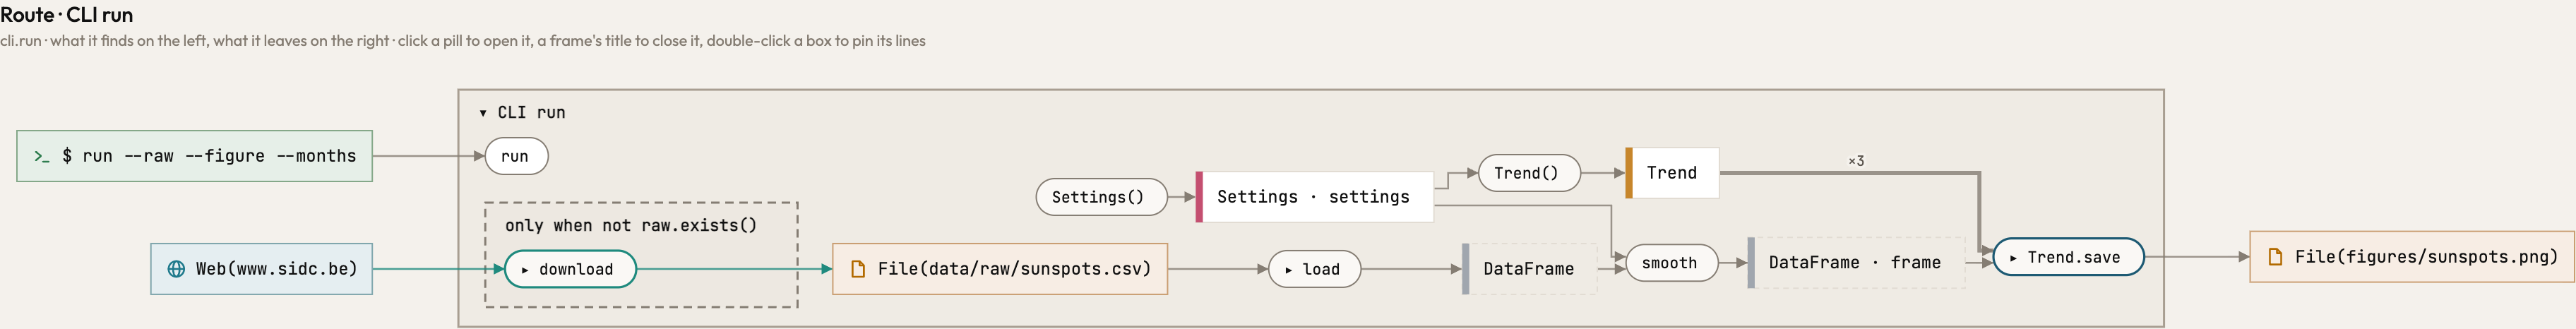
\includegraphics[width=0.9\textheight]{atlas/python-clean.png}}
\caption{The typed program, drawn by atlas. Turned a quarter, because the route is long: read it from bottom to top.}
\label{fig:atlas-clean}
\end{figure}

Both reach the same places: the web, the raw CSV, the figure. Inside they part. In the sloppy script (figure~\ref{fig:atlas-sloppy}) every step reads and changes one global, \texttt{Global(sunspots.df)}, and nothing is handed from step to step. The order in which things must happen is in nobody's signature: you have to know that \texttt{get\_data} runs before \texttt{clean} and \texttt{clean} before \texttt{smooth}, and two of the steps pick their own files. That is the spaghetti of figure~\ref{fig:atlas-shapes}, in a script of a few dozen lines.

In the typed program (figure~\ref{fig:atlas-clean}) you can read the story off the picture. \texttt{download} runs only when there is no raw CSV yet; the CSV stands between \texttt{download} and \texttt{load}; \texttt{load} gives a DataFrame; \texttt{smooth} takes it, together with the settings, and gives a DataFrame with a smoothed column; \texttt{Trend.save} draws that frame into a file. And the command names every file, so you can see where the data comes from and where the figure goes without opening a single function. Same output, same libraries. The difference is entirely in the connections, and the picture shows it in a second.

\subsubsection{A red dot is a question}
Some boxes carry a red dot. A dot is a question atlas asks the author: something in the code does not follow one of the design principles atlas checks. A step reads and changes a global; a function reads a file whose path it chose itself, so nobody calling it can tell where its data comes from; a function's signature doesn't say what it gives. \texttt{atlas check} lists the same questions as text, each with the place in the code, what atlas saw, and a question for you.

A red dot is not a verdict. Atlas coaches; it doesn't fix. Sometimes the answer is to change the code, and the dot disappears. Sometimes the code is right as it is, and then you write that decision down beside the code, with your reason. What I am interested in is that you know which it is, and why. That is the same thing I ask of every number in your report.

Atlas is also not a linter. ruff and ty own the level of lines: style, an unused import, a type that doesn't match. Atlas owns the level above: which steps there are, what travels between them, where data rests. If you make three plots that are really three separate things, the picture should show three separate things; if they come from one preprocessing step, it should show one flow. A linter cannot know which one you meant. Only you can.

\subsection{Working with your agent on the same picture}
\label{sec:atlas-agent}
Your coding agent lives in text, and you are much faster with images. Atlas gives the two of you the same picture. Register it once with your agent (\texttt{claude mcp add -{}-scope user atlas -{}- atlas mcp} for Claude Code), run \texttt{atlas serve} in your repository and open the page it prints. Then you can ask ``where does the smoothing happen?'' and the agent points at the box on your page, instead of describing it. You can write a note on a box (``what happens if the data on the web changes?''), and the agent reads it and answers on the box. And when you ask for a change, the agent can draw it first, beside the code as it is, so you see what it would add before a single file changes. You say yes to a picture, not to a paragraph of text.

This matters for the same reason as everything above. You will write much of your code with an agent, and the danger of that is a fine outside and a mess inside: the plots come out, and nobody, you included, knows how. Looking at the picture together is a way to keep the inside something you understand.

\subsection{Atlas in your final assignment}
\label{sec:atlas-assignment}
Install atlas from \url{https://github.com/raoulg/atlas}; there is an install script for macOS and Linux and one for Windows. In your repository run \texttt{atlas view}, pick the entry point that makes your plots in the dropdown, and open the steps you want to show. Atlas writes one HTML file and keeps your code on your own machine.

In the assessment I will sit next to you and ask you to explain that picture: where your data comes from, which steps it goes through, where each plot is made, and what the red dots ask. You may make your own diagram as well; I will still put atlas next to it, because atlas draws the code you actually wrote, and a diagram can be beautiful and have nothing to do with the code. A tidy picture is easy to explain. If yours looks messy, that is not a failure; it is the question to work on: what would you change in your code so that the picture tells the story you meant? Just as with a model of your data, the aim is not a perfect picture. It is a picture you can explain.

\end{document}
